% The original source files were:
% uiucthesis2009.dtx  (with options: `example')
\def\fileversion{v2.25a} \def\filedate{2009/10/10}
% Package and Class "uiucthesis2009" for use with LaTeX2e.
%%\documentclass[edeposit,fullpage]{latex/uiucthesis2009}
\documentclass[edeposit,fullpage]{uiucthesis2009}

\usepackage{notoccite} % Avoid references in captions causing numbering issues due to TOC
\usepackage{amsmath} % Need for subequations
\usepackage{mathrsfs} %https://ctan.org/pkg/mathrsfs
\usepackage{amssymb} % amssymb-telda and math symbols
\usepackage{booktabs} % Allows fancy Tables
\usepackage{boxedminipage} % Boxes around figures
\usepackage{changepage} % Allows one to temporarily change right and left margins
\usepackage{cite} % Allows improved handling of numeric citations including automatic ordering and ranges of multiple cites
\usepackage{enumitem} % Allows one to easily change the labels for enumerate list
\usepackage[flushleft]{threeparttable} % This package allows for notes under tables.  Flushleft option flushes the note left margin of table (center is default)
% Load tabularx and xcolor before adjustbox to avoid conflict
\usepackage{tabularx} % Package which allows paragraphs in Tables
\usepackage[table]{xcolor} % Allows coloring of tables
\usepackage{graphicx} % Extends graphics package for figures. Provides optional arguments to the \includegraphics command
\graphicspath{{figures/}}
\usepackage[export]{adjustbox} % Extends the graphicx package to do trimming and other adjustments.
\usepackage{epstopdf} % Converts eps images to PDF to use in graphicx package.  Must be loaded after graphicx package
\usepackage[list=true,listformat=simple]{subcaption} % Allow for subfigures with captions in table of contents
\usepackage{bm}
\usepackage{commath}
\usepackage{multirow}

\usepackage{xspace} % Allows dynamic space in global text variables. This can allow you to just use \newCommandName rather than \newCommandName{}.
%%\usepackage[bookmarks=true,backref=page, hyperfigures=true, pdfpagelabels=false]{hyperref}
\usepackage[bookmarks=true,backref=page,hyperfigures=true,pdfpagelabels=false,hidelinks]{hyperref}

\usepackage{bookmark} % Eliminates Warning Bookmark level greater than one. Must be loaded after hyperref
\usepackage[capitalize]{cleveref}% https://ctan.org/pkg/cleveref % Must be loaded after hyperref
\creflabelformat{equation}{#2\textup{#1}#3}% Equation references don't have parentheses
\usepackage[utf8]{inputenc}
\usepackage[nogroupskip,toc,acronym]{glossaries} % place AFTER hyperref for hyperlinked glossary

\usepackage{lineno} % Provide line numbers for drafts

% User defined
% Add you own definitions here (file ANA-STDM-2018-27-INT1-defs.sty).
\usepackage{ANA-STDM-2018-27-INT1-defs}
\usepackage{siunitx} % A units package to format your units properly
\usepackage{atlasparticle}
\usepackage{atlasunit}
%%\usepackage{subfig} % Maybe removed later



%%\usepackage[hidelinks]{hyperref} % remove the colored borders around hyperlinks
%%\linenumbers % uncomment if want draft printing

\begin{document}

\title{Study of Electroweak WW/WZ Production in the Semileptonic Final States in Association with a High-mass Dijet System using the ATLAS Detector}
\author{JianCong Zeng}
\department{Physics}
\schools{B.A. in Physics, The State University of New York College at Geneseo}
\phdthesis
\advisor{Dr. Mark Neubauer}
\degreeyear{2024}
\committee{Associate Professor Benjamin Hooberman, Chair\\
           Professor Mark Neubauer, Director of Research\\
           Professor Brian D. Fields\\
           Assistant Professor Yonatan Frederick Kahn}
\maketitle

\frontmatter

% Create an abstract that can also be used for the ProQuest abstract.
% Note that ProQuest truncates their abstracts at 350 words.
\begin{abstract}
The analysis searches for electroweak diboson ($WW/WZ/ZZ$) production in association with a high-mass dijet system, using data from proton-proton collisions at a center-of-mass energy of $\sqrt{s} = 13 TeV$. The analysis is performed in the semi-leptonic final states which include a hadronic decay boson and a leptonic decay one. The analysis is split into three channels according to the number of electrically charged leptons from the leptonic boson decay: 0-lepton channel, 1-lepton channel, and 2-lepton channel.
The focus of this thesis is an approach to enhance the separation between the VBS signal and the backgrounds in the 1-lepton channel using artificial neural network models. This approach is developed using Monte Carlo simulated events in the semi-leptonic VBS analysis and tested using ATLAS data for improving the sensitivity of the analysis to the target signal.
\end{abstract}

% Create a dedication in italics with no heading, centered vertically
% on the page.
\begin{dedication}
Write Dedication Here
\end{dedication}

% Create an Acknowledgements page, many departments require you to
% include funding support in this.
\chapter*{Acknowledgments}
This work was supported by the U.S. Department of Energy, Office of Science, High Energy Physics, under contract number DE-SC0023365.

Mark Neubauer, Viviana Cavelier, Matthew Feickert

Also, I would like to say thank you to my late grandparents. Though you might not have fully understood my work, I am grateful for every memory we shared. Finally, to my parents, Meizhen Zhu and Yuesong Zeng, who moved across continents to allow me to fulfill my dream of becoming a physicist: It has been a long journey, and I cannot thank you enough for your unwavering support and patience. There is still a long journey ahead of me, and I am determined to make you proud with every step I take.


% The thesis format requires the Table of Contents to come
% before any other major sections, all of these sections after
% the Table of Contents must be listed therein (i.e., use \chapter,
% not \chapter*).  Common sections to have between the Table of
% Contents and the main text are:
%
% List of Tables
% List of Figures
% List Symbols and/or Abbreviations
% etc.

{
    \hypersetup{linkcolor=black}  % disable link coloring locally
    \setcounter{tocdepth}{2}
    \tableofcontents
    % the Graduate College doesn't recommend including lot or lof
    % \listoftables
    % \listoffigures
}

%\tableofcontents
%\listoftables
%\listoffigures
%%% Create a List of Abbreviations. The left column
%% is 1 inch wide and left-justified
\chapter{List of Abbreviations}

%% List of Abbreviations, edit as needed
\begin{symbollist*}
\item[2HDM] Two-Higgs Doublet Model.
\item[AK4] An anti-$k_t$ jet with $R = 0.4$.
\item[ALICE] A Large Ion Collider Experiment.
\item[AM] Associated Memory.
\item[AMB] Associated Memory Board.
\item[ATCA] Advanced Telecommunications Computing Architecture.
\item[ATLAS] A Toroidal LHC ApparatuS.
\item[AUX] Auxiliary Board.
\item[AXW] AUX Wrapper.
\item[BR] Branching Ratio.
\item[CA12] A Cambridge/Aachen jet with $R = 1.2$.
\item[CC] Clock Correction.
\item[CERN] European Organization for Nuclear Research.
\item[CL] Confidence Level.
\item[CMS] Compact Muon Solenoid.
\item[CP] Combined Performance.
\item[CR] Control Region.
\item[DF] Data Formatter.
\item[DFW] DF Wrapper.
\item[DRAM] Dynamic Random Access Memory.
\item[DSP] Digital Signal Processing Block.
\item[ECAL] Electromagnetic Calorimeter.
\item[ECR] Event Count Reset.
\item[EGM] Extended Gauge Model.
\item[EF] Event Filter.
\item[ELID] Extended Level 1 Identifier.
\item[EXP] Extrapolator.
\item[EXTF] Extrapolator / Track Fitter.
\item[FC] Flow Control.
\item[FCAL] Forward Calorimeter.
\item[FE] Front End.
\item[FF] Flip Flop.
\item[FIFO] First In First Out.
\item[FLIC] FTK Level-2 Interface Crate.
\item[FPGA] Field Programmable Gate Array.
\item[FSR] Final State Radiation
\item[fSSB] Final Second Stage Board.
\item[FTK] Fast TracKer.
\item[GTX] Gigabit Transceiver.
\item[ggF] gluon Fusion.
\item[HEP] High Energy Physics.
\item[HLT] High Level Trigger.
\item[HP] High Purity.
\item[HVT] Heavy Vector Triplet.
\item[HW] Hit Warrior.
\item[HXMPP] Hit Memory++.
\item[IBL] Insertable B Layer.
\item[ID] Inner Detector.
\item[IM] Input Mezzanine.
\item[ISR] Initial State Radiation.
\item[JVF] Jet Vertex Fraction.
\item[JER] Jet Energy Resolution.
\item[JES] Jet Energy Scale.
\item[KK] Kaluza-Klein.
\item[L1] Level 1 Hardware Trigger.
\item[L2] Level 2 Hardware Trigger.
\item[LAMB] Local Associated Memory Board.
\item[LDC] Link Destination Card.
\item[LED] Light Emitting Diode.
\item[LFSR] Linear Feedback Shift Register.
\item[LHC] Large Hadron Collider.
\item[LHCb] Large Hadron Collider beauty.
\item[LINAC2] Linear Accelerator 2.
\item[LP] Low Purity.
\item[LSC] Link Source Card.
\item[LUT] Look Up Table.
\item[MC] Monte Carlo.
\item[MET] Missing Transverse Energy.
\item[MIG] Memory Interface.
\item[ML] Maximum Likelihood.
\item[MS] Muon Spectrometer.
\item[NLO] Next to Leading Order.
\item[NNLO] Next to Next to Leading Order.
\item[PDF] Parton Distribution Function.
\item[PIX] Pixel Detector.
\item[PU] Processing Units.
\item[PS] Proton Synchrotron.
\item[pSSB] Preliminary Second Stage Board.
\item[QCD] Quantum Chromo Dynamics.
\item[QSFP] Quad Small Form-factor Pluggable.
\item[RAM] Read Access Memory.
\item[RLDRAM] Reduced Latency DRAM.
\item[ROD] Read Out Driver.
\item[ROI] Region of Interest.
\item[ROM] Read Only Memory.
\item[ROS] Read Out System.
\item[RS] Randall-Sundrum.
\item[RTM] Rear Transmission Module.
\item[RX] Receiver.
\item[SCT] Semiconductor Tracker.
\item[SE] Sync Engine.
\item[SF] Scale Factor.
\item[SFP] Small Form-factor Pluggable.
\item[SLink] Super Link.
\item[SM] Standard Model.
\item[SPS] Super Proton Synchrotron.
\item[SR] Signal Region.
\item[SSB] Second Stage Board.
\item[SSID] Super Strip Identifier.
\item[TDAQ] Trigger and Data Acquisition.
\item[TF] Track Fitter.
\item[TFW] Track Fitter Wrapper.
\item[TileCAL] Hadronic Calorimeter.
\item[TRT] Transition Radiation Tracker.
\item[TX] Transmitter.
\item[VBF] Vector Boson Fusion.
\item[VME] VERSA-Module Euro.
\item[VR] Validation Region.
\end{symbollist*}

%% Symbol defs
\def\met{\ensuremath{E_{\mathrm{T}}^{\mathrm{miss}}}}

%% Create a List of Symbols. The left column
%% is 0.7 inch wide and centered
%% Edit as needed

\chapter{List of Symbols}

\begin{symbollist}[0.7in]
    \item[$\ell$] lepton.
    \item[$e$] electron.
    \item[$\mu$] muon.
    \item[$\tau$] tau.
    \item[$\nu_{e}$] electron neutrino.
    \item[$\nu_{\mu}$] muon neutrino.
    \item[$\nu_{\tau}$] tau neutrino.
    \item[$q$] quark, also used for charge.
    \item[$u$] up quark.
    \item[$d$] down quark.
    \item[$s$] strange quark.
    \item[$c$] charm quark.
    \item[$b$] bottom quark.
    \item[$t$] top quark.
    \item[$g$] gluon.
    \item[$\gamma$] photon.
    \item[$W$] $W$ boson.
    \item[$Z$] $Z$ boson.
    \item[$H$] Higgs boson.
    \item[$V$] Vector boson.
    \item[$p$] proton.
    \item[$n$] neutron.
    \item[$G^*$] RS graviton.
    \item[$G_{KK}$] KK graviton.
    \item[$W'$] Heavy $W$ boson.
    \item[$Z'$] Heavy $Z$ boson.
    \item[$V'$] Heavy Vector Boson.
    \item[$E_T^{miss}$] Missing transverse energy.
    \item[$E_T$] Transverse energy.
    \item[$p_T$] Transverse momentum.
    \item[$\eta$] pseudo rapidity.
    \item[$\theta$] polar angle.
    \item[$\phi$] azimuthal angle.
    \item[$d_0$] the distance to the $z$-axis at the perigee point.
    \item[$z_0$] the $z$-coordinate at the perigee point.
    \item[$\phi_0$] the azimuthal angle at the perigee point.
    \item[$\chi^2$] statistic that measures how good the data fits the track.
    \item[$R$] distance in $\eta-\phi$ space.
    \item[$j$] small-$R$ jet.
    \item[$J$] large-$R$ jet.
    \item[$g_f$] fermion coupling.
    \item[$g_H$] Higgs and vector boson coupling.
    \item[$g_\ell$] lepton coupling.
    \item[$g_q$] quark coupling.
    \item[$\sigma$] cross section.
    \item[$m$] mass.
    \item[fb] femto barn $= 10^{-43}~\mathrm{m}^2$.
    \item[eV] electron Volt $= 1.602 \times 10^{-19}~\mathrm{J}$.
\end{symbollist}


\mainmatter

\chapter{Introduction}
%%% introduction %%%

The investigation of electroweak symmetry breaking (EWSB) has been one of the pivotal objectives of experiments conducted at the Large Hadron Collider (LHC). 
Within the Standard Model (SM) of particle physics, EWSB is explained by the Brout-Englert-Higgs mechanism, a cornerstone of our understanding of particle interactions~\cite{Englert:1964et,Higgs:1964pj,Guralnik:1964eu}. 
While the Higgs boson's discovery and subsequent measurements have significantly advanced our knowledge, a comprehensive understanding of EWSB requires further investigation.
Vector boson scattering (VBS) plays a crucial role in this context, owing to its sensitivity to the interactions involving the longitudinal components of gauge bosons, which are directly tied to the mechanism of EWSB.

The ATLAS and CMS collaborations have reported results from their fully leptonic VBS analyses conducted during the LHC's Run-II period. These findings, detailed in a series of publications by ATLAS~\cite{STDM-2017-19, STDM-2017-06, STDM-2017-23} and by CMS~\cite{2021135992, 2022137438}, have led to the official claim of observing the SM VBS process with fully leptonic final states.

In the study of VBS, Beyond Standard Model (BSM) physics is often explored through the effective field theory (EFT) framework~\cite{Longhitano:1980tm}. Within this framework, VBS interactions can be influenced by anomalous quartic gauge couplings (aQGCs). Searches for evidence of aQGCs have been conducted across various experiments. These efforts are part of a continuing exploration to understand the potential for new physics beyond what the SM currently describes.
aQGCs typically cause an increase in the VBS cross-section. This enhancement is noticeable at high transverse momentum (\pt) of the vector bosons and at high invariant mass of the two-boson system.

Experimentally, VBS is recognized by two key features: the presence of a pair of vector bosons ($W$, $Z$, or $\gamma$) and two forward jets. These jets are notably separated by a large distance in rapidity and have a high dijet invariant mass. Previous studies searching for aQGCs in VBS events have mainly focused on cases where the bosons decay into leptons ($W(l\nu)$ and $Z(ll)$)~\footnote{Unless otherwise noted, $\ell$ stands for either electron ($e$) or muon ($\mu$) in this thesis.} and photons.

The semi-leptonic channels, such as $V(qq')Z(\nu\nu)$, $V(qq')W(l\nu)$ and $V(qq')Z(ll)$ (V = W, Z), present unique advantages. 
The branching fractions—meaning the probabilities of these decay modes—are much larger for decays involving $V(qq')$ compared to those that are purely leptonic. 
%Furthermore, jet substructure techniques, which analyze the internal structure of jets, enable efficient reconstruction of these events at high \pt, an area highly sensitive to aQGCs. 
This efficiency and sensitivity make the semi-leptonic channels particularly appealing for aQGC searches.

This thesis focuses on analyzing the production of $V(qq')W(l\nu)$ alongside a high-mass dijet system, in a phase space optimized for sensitivity to VBS and aQGCs. This specific setup is referred to as the 1-lepton channel, part of a broader analysis that includes 0-lepton, 1-lepton, and 2-lepton channels~\cite{Charlton:2808769}. The primary emphasis is on the 1-lepton channel, showcasing a machine learning approach designed to improve the detection sensitivity to SM VBS process.

This thesis is structured as follows: Chapter~\ref{ch:theory_overview} offers a brief overview of the Standard Model, delves into the physics of the Higgs field, and explains why searching for VBS and aQGCs is important.
Chapter~\ref{ch:Experimental_Apparatus} describes the experimental setup used to gather the data for this study, focus on the LHC and the ATLAS detector. Chapters~\ref{ch:exp_methods} to~\ref{ch:stat_interpretation} detail the entire workflow of the semi-leptonic VBS analysis and highlight the promising outcomes achieved using my machine learning approach.




\chapter{Theoretical Overview}
%%%Theory
\label{ch:theory_overview}

The Standard Model of particle physics is our best description of elementary particles and how they interact. The SM has been tested and proven right by many experiments worldwide at various energy levels. Even though the SM has been very successful, it doesn't answer every question about the universe, leaving space for new theories beyond the SM that try to fill these gaps and explain the mysteries. This chapter gives a simple overview of the SM, discusses the importance of the Higgs field, and explains why studying VBS and aQGCs is essential.

\section{Standard Model}
The Standard Model of particle physics offers a comprehensive framework that describe the fundamental particles and the interactions governing them, excluding gravity~\cite{PeskinSchroeder1995}. 
Table~\ref{table:fundamental_forces} shows the relative strengths of these four fundamental forces, highlighting the marked disparity between gravity and the other forces within the realm of subatomic particles.


\begin{table}[h]
\centering
\begin{tabular}{|l|l|}
\hline
\textbf{Force}         & \textbf{Relative Strength} \\ \hline
Strong Nuclear Force   & 1                          \\ \hline
Electromagnetic Force  & \textasciitilde{}1/137     \\ \hline
Weak Nuclear Force     & \textasciitilde{}10\(^{-6}\) \\ \hline
Gravitational Force    & \textasciitilde{}10\(^{-38}\) \\ \hline
\end{tabular}
\caption{Relative Strengths of the Fundamental Forces}
\label{table:fundamental_forces}
\end{table}


The particles of the Standard Model are classified into four distinct categories. Leptons and quarks constitute all known matter, each possessing half-integer spin and adhering to Fermi-Dirac statistics. This principle prohibits any two identical fermions from occupying identical quantum states simultaneously. The model includes six leptons and six quarks, each accompanied by a corresponding antiparticle counterpart. A fundamental distinction between these particle types is that quarks are subject to the strong nuclear force, whereas leptons are not. Furthermore, quarks are perpetually bound within composite particles known as hadrons—protons and neutrons being the most recognized examples.

The remaining particles within the Standard Model facilitate the interactions among leptons and quarks and are characterized by integer spin, thereby following Bose-Einstein statistics. This group encompasses the gauge bosons, which are spin-1 particles responsible for mediating the three fundamental forces, and the Higgs boson~\cite{Higgs:1964ia}, a unique scalar particle with a spin-0, crucial for imparting mass to other particles. 
Figure \label{fig:stdm_higgs} and Table~\ref{table:SMparticles} show all Standard Model particles, alongside their properties.

%figures/theory/STDM_higgs.png

\begin{figure}[ht]
    \centering
%%    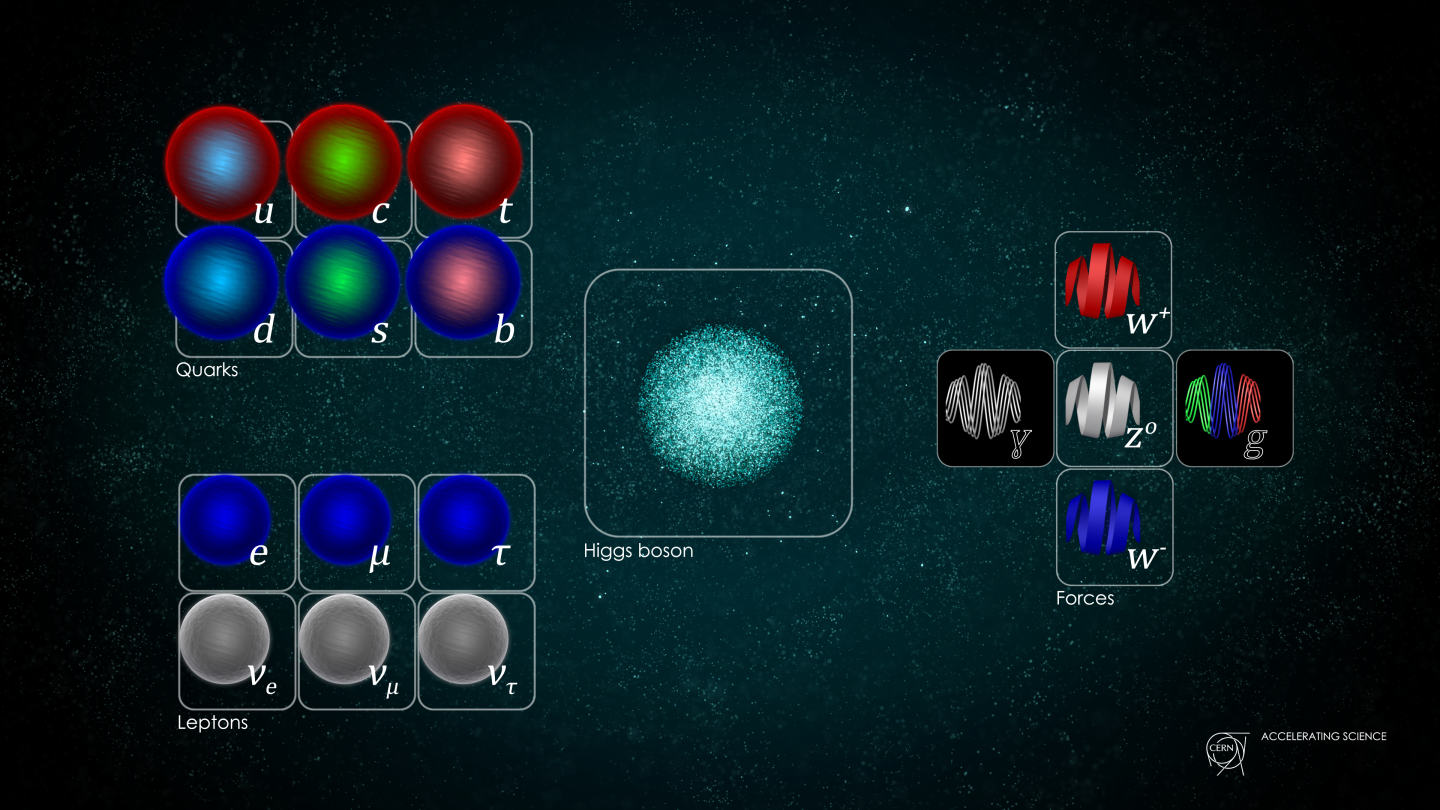
\includegraphics[width=0.95\textwidth]{figures/theory/STDM_higgs.png}
    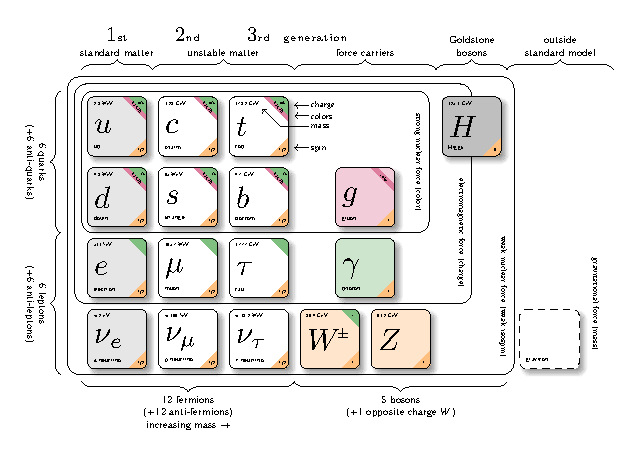
\includegraphics[width=0.95\textwidth]{figures/theory/model-physics.pdf}
    \caption{Illustration of Standard Model particles~\cite{Burgard2019}.}
    \label{fig:stdm_higgs}
\end{figure}

\begin{table}[ht]
\centering
\begin{tabular}{|l|l|l|l|l|}
\hline
\textbf{Particle Type} & \textbf{Particle} & \textbf{Spin} & \textbf{Charge (e)} & \textbf{Mass}            \\ \hline
\multirow{6}{*}{Lepton}& Electron (e\(^-\))        & 1/2           & -1               & 0.511 MeV/c\(^2\)        \\ \cline{2-5}
                       & Muon (\(\mu^-\))          & 1/2           & -1               & 105.7 MeV/c\(^2\)        \\ \cline{2-5}
                       & Tau (\(\tau^-\))          & 1/2           & -1               & 1.777 GeV/c\(^2\)        \\ \cline{2-5}
                       & Electron Neutrino (\(\nu_e\))    & 1/2           & 0                & $< 2 \, \text{eV}/c^2$           \\ \cline{2-5}
                       & Muon Neutrino (\(\nu_{\mu}\))    & 1/2           & 0                & $< 0.19 \, \text{MeV}/c^2$       \\ \cline{2-5}
                       & Tau Neutrino (\(\nu_{\tau}\))    & 1/2           & 0                & $< 18.2 \, \text{MeV}/c^2$       \\ \hline
\multirow{6}{*}{Quark} & Up (u)                & 1/2           & +2/3              & 2.3 MeV/c\(^2\)          \\ \cline{2-5}
                       & Down (d)              & 1/2           & -1/3              & 4.8 MeV/c\(^2\)          \\ \cline{2-5}
                       & Charm (c)             & 1/2           & +2/3              & 1.275 GeV/c\(^2\)        \\ \cline{2-5}
                       & Strange (s)           & 1/2           & -1/3              & 95 MeV/c\(^2\)           \\ \cline{2-5}
                       & Top (t)               & 1/2           & +2/3              & 173.1 GeV/c\(^2\)        \\ \cline{2-5}
                       & Bottom (b)            & 1/2           & -1/3              & 4.18 GeV/c\(^2\)         \\ \hline
\multirow{4}{*}{Gauge Boson} & Photon (\(\gamma\))         & 1             & 0                & 0                        \\ \cline{2-5}
                       & W Boson (W\(^{\pm}\))       & 1             & \(\pm 1\)        & 80.379 GeV/c\(^2\)       \\ \cline{2-5}
                       & Z Boson (Z\(^0\))          & 1             & 0                & 91.1876 GeV/c\(^2\)       \\ \cline{2-5}
                       & Gluon (g)             & 1             & 0                & 0                         \\ \hline
Scalar Boson           & Higgs (H)             & 0             & 0                & 125.10 GeV/c\(^2\)       \\ \hline
\end{tabular}
\caption{Standard Model Particles and Their Known Properties.}
\label{table:SMparticles}
\end{table}

The SM is a quantum field theory anchored in the symmetry group $\mathrm{SU}(3)_C \otimes \mathrm{SU}(2)_L \otimes \mathrm{U}(1)_Y$, where each component of the symmetry group governs a different aspect of particle interactions. In this context, the $\mathrm{SU}(3)_C$ symmetry relates to the strong interaction, with the subscript $C$ denoting color charge—a conserved property. Color charge exists in three forms—red, blue, and green—alongside their anticolors (anti-red, anti-blue, and anti-green). 

One of the foundational principles of quantum chromodynamics (QCD)~\cite{CampbellHustonKrauss2017}, the theory of the strong interaction, is that color charge is never observed in isolation. This phenomenon, known as color confinement, dictates that quarks are always found in composite particles called hadrons, which exhibit a neutral color charge. 
Hadrons are categorized into mesons and baryons. Mesons consist of a quark and an antiquark pair, combining a color with its anticolor. Baryons, such as the proton and neutron, are formed from three quarks, each of a distinct color (or anticolor), which collectively neutralize their color charge. This configuration explains why hadrons are observable in nature, contrary to isolated quarks.
As quarks attempt to separate, they undergo a process known as \emph{hadronization}. During hadronization, new quark-antiquark pairs spontaneously emerge from the vacuum. These new particles arrange themselves to neutralize the color charge of the initially separating quarks. As a result, instead of isolated quarks, we observe the formation of new hadrons, ensuring that the color charge remains confined.
Hadronization and its resulting particle decays produce a shower(cascade) of hadrons and leptons known as a ``jet.'' These jets, which will be discussed on in Section~\ref{subsec:jet_selection}, are crucial for probing QCD physics. 

The electroweak interaction, described by the symmetry group $\mathrm{SU}(2)_L \times \mathrm{U}(1)_Y$, unifies the electromagnetic and weak forces~\cite{GLASHOW1961579, PhysRev.127.965, PhysRevLett.19.1264}. The conservation of electric charge ($Q$) is central to this theory, governed by the formula: $Q = \frac{Y}{2} + T_3$. Here, $Y$ denotes the hypercharge, and $T_3$ is the third component of the weak isospin ($T$), akin to the third component of spin in quantum mechanics, differentiating ``up'' and ``down'' states within isospin doublets. This framework introduces a distinction in symmetry for particles based on their chirality: left-handed particles exhibit doublet configurations under $\mathrm{SU}(2)_L$, while right-handed particles form singlets, indicating they do not participate in weak isospin doublets. 

Spin-1 particles, known as gauge bosons or vector bosons, are the force carriers in the SM. The photon mediates the electromagnetic force. The weak force is mediated by three vector bosons, the $W^{\pm}$ and $Z$ bosons. For the strong force, it is mediated by eight different gluons. A key feature of the weak force is lepton universality, meaning all types of leptons couple to the $W^{\pm}$ and $Z$ bosons in the same way, leading to identical branching ratios for each lepton type.

\section{The Higgs Mechanism}

%%%Higgs

In the SM, the requirement of gauge invariance under the group $\mathrm{SU}(2)_L \otimes \mathrm{U}(1)_Y$ implies that weak bosons and fermions should be massless. However, this stands in contradiction to the observed masses of these particles. 
The resolution within the SM framework is the Higgs mechanism \cite{Higgs:1964ia, PhysRevLett.13.508, PhysRevLett.13.321, PhysRevLett.13.585}, which introduces the Higgs field. Through spontaneous symmetry breaking, this scalar field gives mass to the weak bosons and fermions, reconciling the SM with experimental observations.

Spontaneous symmetry breaking refers to a phenomenon where the ground state of a symmetric system does not reflect the system's symmetry after perturbation. The term ``breaking'' does not imply the destruction of the Lagrangian symmetry. Instead, the symmetry is not apparent in the perturbed ground state of the system.
A classical example of spontaneous symmetry breaking is the magnetization of iron. Above its Curie temperature, iron's magnetic moments are oriented randomly, respecting rotational symmetry. Upon cooling below this temperature, the moments align uniformly, creating a magnet with distinct poles. Although the magnet displays a specific orientation, the physical principles governing magnetism retain their inherent symmetry.

The scalar field (Higgs field), $\phi$, represented as a complex doublet, takes on a non-zero vacuum expectation value (VEV) of $v \approx 246$ GeV, leading to three massive gauge bosons ($W^{\pm}$ and $Z$) and the Higgs boson ($H$).

% The complex scalar doublet
\begin{equation}
\phi =
\begin{pmatrix}
\phi^+ \\
\phi^0
\end{pmatrix}
=
\frac{1}{\sqrt{2}}
\begin{pmatrix}
\phi_1 + i\phi_2 \\
\phi_3 + i\phi_4
\end{pmatrix}
\end{equation}



The Lagrangian density of the Higgs field, $\mathcal{L}_\text{Higgs}$, respects local $\mathrm{SU}(2)_L \otimes \mathrm{U}(1)_Y$ symmetry and includes the Higgs potential $V(\phi)$, as shown in Figure~\ref{fig:higgs_potential}. This potential is defined with parameters $\mu^2 < 0$ and $\lambda > 0$ to ensure stable minima. 
% The Lagrangian density
\begin{equation}
\mathcal{L}_\text{Higgs} = (D^\mu\phi)^\dagger (D_\mu\phi) - V(\phi),
\end{equation}
where \(V(\phi)\) is the Higgs potential, given by
\begin{equation}
V(\phi) = \mu^2\phi^\dagger\phi + \lambda (\phi^\dagger\phi)^2.
\end{equation}

\begin{figure}[ht]
\centering
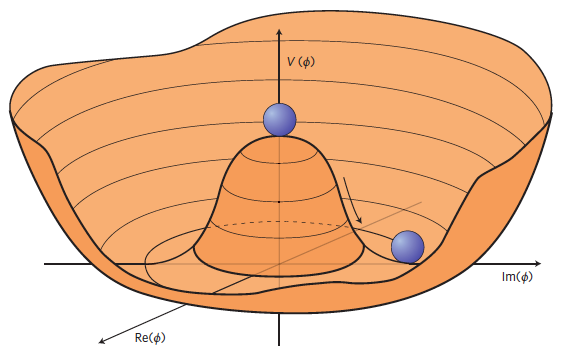
\includegraphics[width=0.75\textwidth]{figures/theory/higgspotential.png}
\caption[Higgs Potential]{The Higgs potential, adapted from Ellis (2013) \cite{ellis2013higgs}.}
\label{fig:higgs_potential}
\end{figure}

Choosing a ground state breaks the $\mathrm{SU}(2)_L \otimes \mathrm{U}(1)_Y$ symmetry to the subgroup $\mathrm{U}(1)_\text{QED}$, reparameterizing the complex scalar doublet's components into observable fields.
After this symmetry breaking, the scalar doublet fields are reparameterized as:
\begin{equation}
\phi(x) = \frac{1}{\sqrt{2}}
\begin{pmatrix}
0 \\
v + h(x)
\end{pmatrix}
\exp\left( \frac{i \tau^i \phi^i(x)}{2} \right),
\end{equation}
where $h(x)$ is the Higgs boson field, and the $\phi^i(x)$ are the Goldstone bosons that become gauge degrees of freedom in the unitary gauge $\phi^i(x) = 0$. This simplifies the kinetic term of the Lagrangian, resulting in mass terms for the $W^\pm$ and $Z$ bosons as:
\begin{equation}
m_W = \frac{1}{2}vg, \quad m_Z = \frac{vg}{2\cos\theta_W}.
\end{equation}
The Higgs boson mass is determined as:
\begin{equation}
m_h = \sqrt{-2\mu^2} = v\sqrt{2\lambda}.
\end{equation}

In the SM, the VEV of the Higgs field, denoted by \( v \), along with the gauge coupling constants \( g_1 \) and \( g_2 \), are free parameters. These are not predicted by the theory but are determined through experimental measurements. The VEV has been established to be about 246 GeV~\cite{Plehn_2005}. This VEV is crucial as it gives mass to the $W^\pm$ and $Z$ bosons through the mechanism previously discussed.

Quarks and charged leptons also gain their mass by interacting with the Higgs field. These interactions are described by Yukawa couplings~\cite{10.1143/PTPS.1.1}.
Each type of fermion has its own Yukawa coupling constant \( c_i \), which determines the strength of its interaction with the Higgs field, and therefore, its mass.


\begin{equation}
\mathcal{L}_\text{Yukawa} = -\frac{1}{\sqrt{2}} (v + h)(c_{1} \bar{d}d + c_{2} \bar{u}u + c_{3} \bar{e}e)
\end{equation}

\begin{equation}
= -\left( 1 + \frac{h}{v} \right)(m_{d} \bar{d}d + m_{u} \bar{u}u + m_{e} \bar{e}e) .
\end{equation}


Neutrinos, however, do not acquire mass through the same mechanism. They remain massless in the SM's framework of electroweak symmetry breaking. The fact that neutrinos have been observed to have mass in experiments is an unsolved issue within the SM, hinting at new physics beyond the current theory.

\section{Vector Boson Scattering}
%%%VBS Theory
%\section{Vector Boson Scattering}
\label{section:Vector_Boson_Scattering}

When the scalar field \( \phi \) is expanded around its ground state value, the kinetic term in $\mathcal{L}_\text{Higgs}$ becomes

\begin{equation}
|D_\mu \phi|^2 = \frac{1}{2} (\partial_\mu \phi_0)^2 + \frac{1}{2} (\partial_\mu \phi_2)^2 
+ g^2 \phi_0^2 A_\mu A^\mu + \sqrt{2} g \phi_0 A_\mu \partial^\mu \phi_2 + \ldots,
\end{equation}
where the mass term for \( A_\mu \) is \( g^2 \phi_0^2 A_\mu A^\mu \). The term \( \sqrt{2} g \phi_0 A_\mu \partial^\mu \phi_2 \) provides an extra degree of freedom for \( A_\mu \). The directly coupling \( A_\mu \) to \( \phi_2 \) allows \( \phi_2 \) to serve as an additional degree of freedom for the gauge boson \( A_\mu \), enabling it to acquire the necessary longitudinal polarization to be a massive particle.

A vector boson is a boson with spin-1. By definition, the gauge bosons mentioned above are vector bosons, which introduces Vector Boson Scattering (VBS) into the discussion. 
The SM VBS process involves a quartic gauge coupling (QGC) vertex, as shown in Figure~\ref{fig:qgc_vertex}, which depicts the self-coupling among four electroweak gauge bosons.
The discovery of a Higgs boson in LHC~\cite{20121, 201230} motivates further study of the mechanism of EWSB by probing the VBS processes.
Given that new physics in the electroweak sector is likely to involve QGCs,
the measurements of VBS at high energy are crucial tests of the SM and will determine whether the Higgs is entirely responsible for EWSB.

\begin{figure}[tbp]
\centering
\subfloat[]{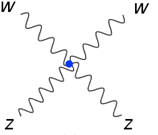
\includegraphics[width=0.27\textwidth]{figures/theory/qgc_1.png}}
\hfill
\subfloat[]{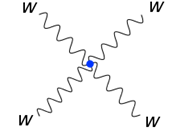
\includegraphics[width=0.3\textwidth]{figures/theory/qgc_2.png}}
\hfill
\subfloat[]{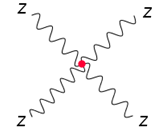
\includegraphics[width=0.27\textwidth]{figures/theory/qgc_3.png}}
\caption{Examples of QGC vertices: (a) and (b) are within the SM; (c) is anomalous, discussed further in Section~\ref{Anomalous_Quartic_Gauge_Couplings}. These and other Feynman diagrams in this thesis are made using the JaxoDraw~\cite{Binosi:2003yf} program.}
\label{fig:qgc_vertex}
\end{figure}

In Figure~\ref{fig:feynmanVBS}, we present examples of VBS diagrams that contribute to the SM signal process in the analysis. 
In the Feynman diagrams presented, a dashed line represents the Higgs boson, a solid line represents quark, and a rippled line represents vector boson.
It's noteworthy that not all VBS diagrams involve quartic gauge couplings. The decays of the bosons are not explicitly shown.

In Figure~\ref{fig:feynmanEWKnonVBS}, we present several non-VBS electroweak diagrams. These include purely-electroweak tree-level diagrams, specifically of order $\mathcal{O}(\alpha_{EW}^6)$, contributing to the final state. Such non-VBS diagrams are expected to be significantly suppressed by the event selection criteria employed in this analysis.

%% feynman diagrams, VBS
%
\begin{figure}[tbp]
\begin{center}
\subfloat[]{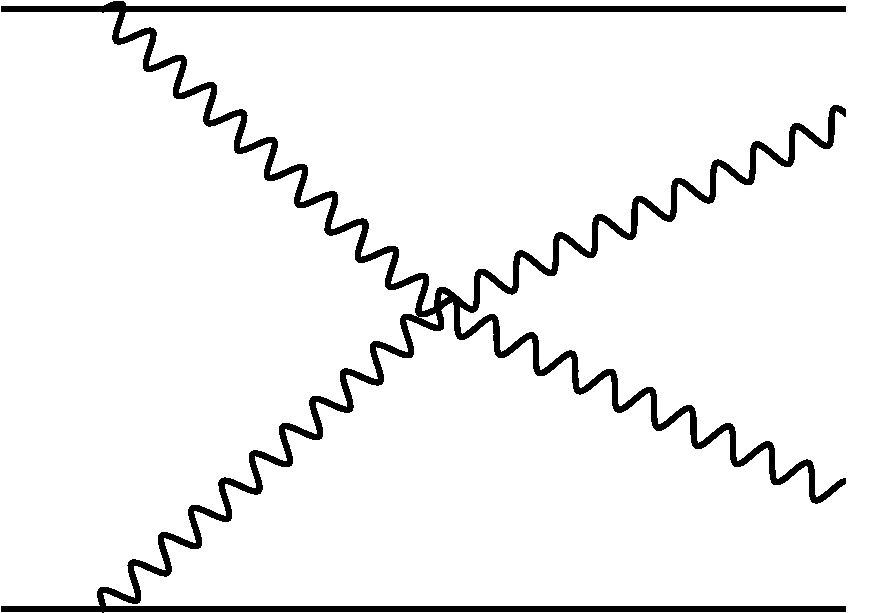
\includegraphics[width=0.3\textwidth]{figures/samples/feynVBS2.pdf}}
\subfloat[]{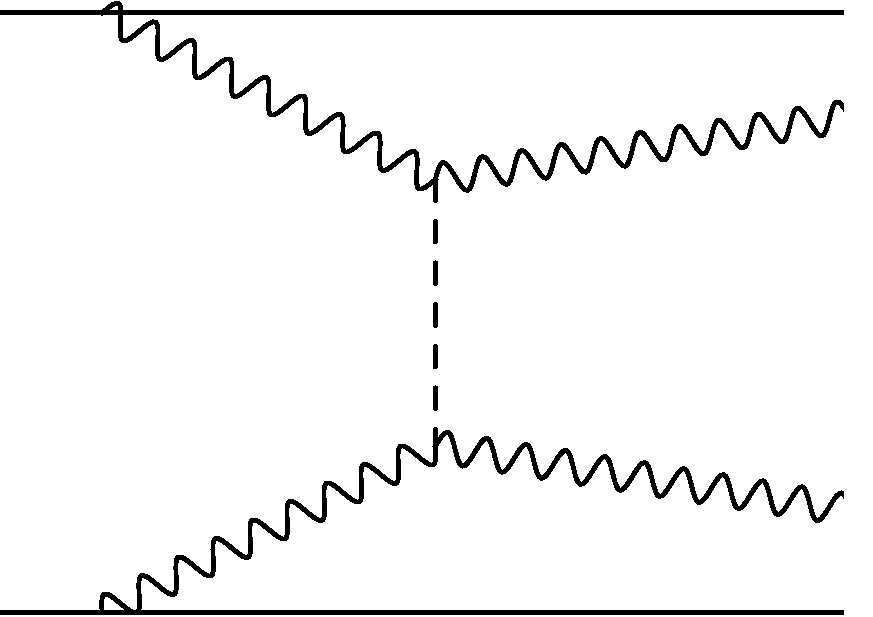
\includegraphics[width=0.3\textwidth]{figures/samples/feynVBS1.pdf}}
\subfloat[]{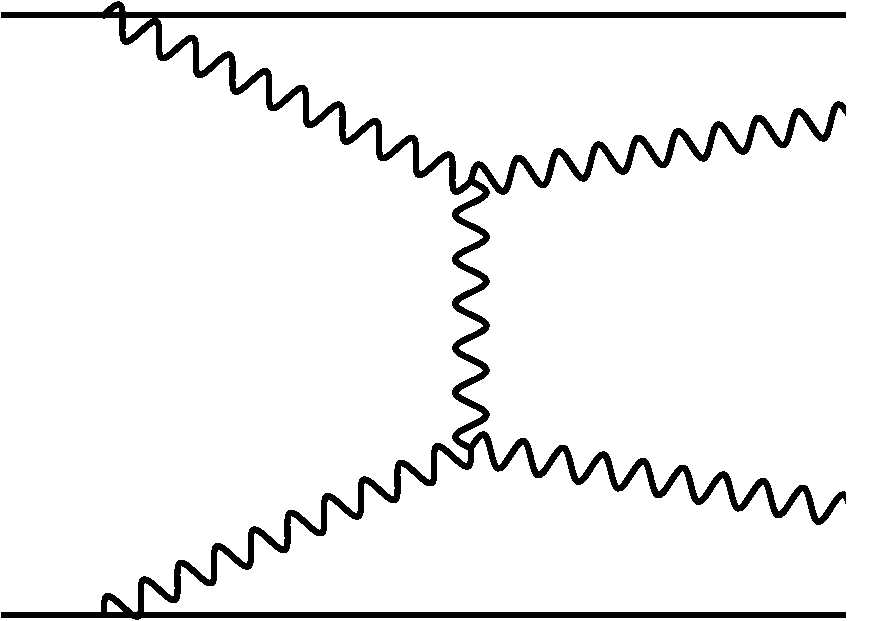
\includegraphics[width=0.3\textwidth]{figures/samples/feynVBS3.pdf}}\\
\subfloat[]{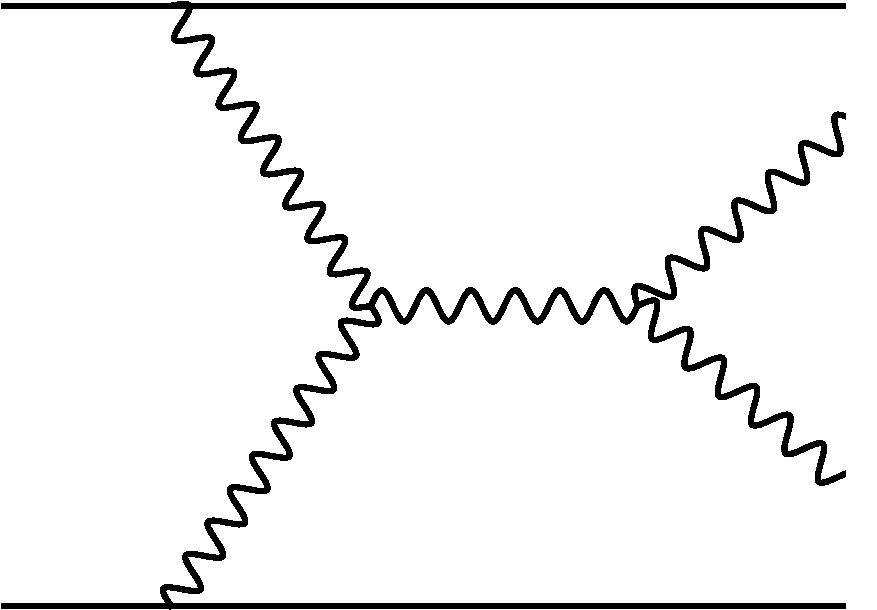
\includegraphics[width=0.3\textwidth]{figures/samples/feynVBS4.pdf}}
\subfloat[]{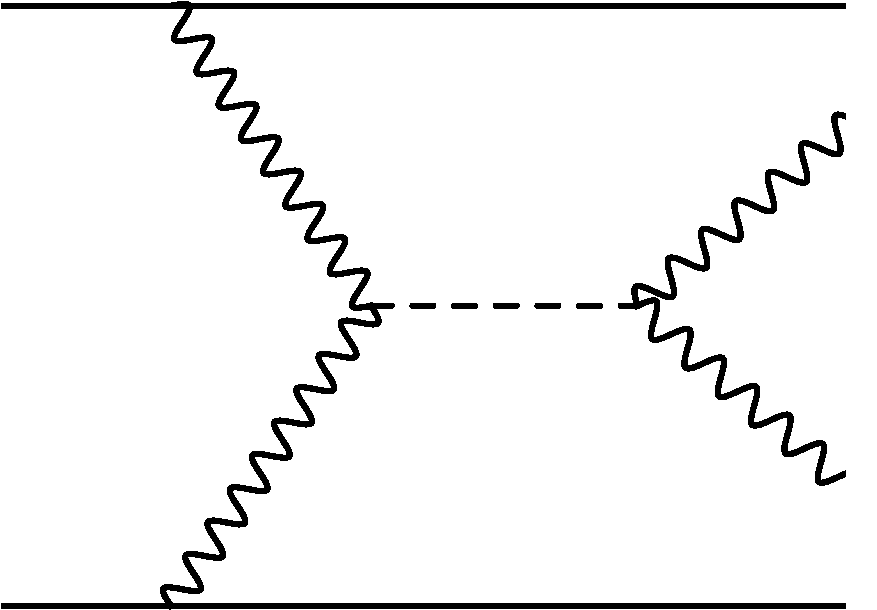
\includegraphics[width=0.3\textwidth]{figures/samples/feynVBS5.pdf}}
\caption{
Examples of VBS diagrams contributing to the signal. Note that not all VBS diagrams contain quartic gauge couplings.
}
\label{fig:feynmanVBS}
\end{center}
\end{figure}


%% feynman diagrams, non-VBS
%
\begin{figure}[tbp]
\begin{center}
\subfloat[]{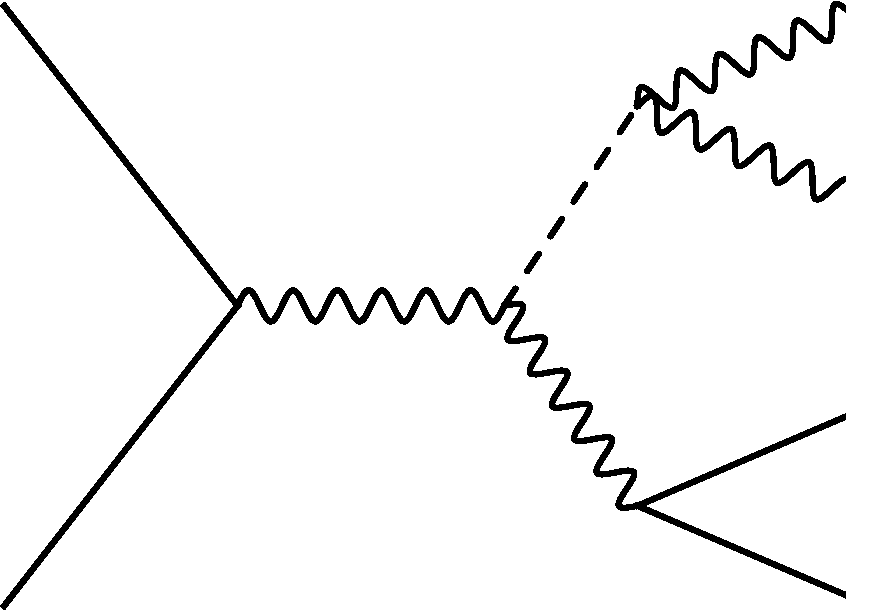
\includegraphics[width=0.3\textwidth]{figures/samples/feynEWKnonVBS3.pdf}}
\subfloat[\label{subfig:feynEWKnonVBSb}]{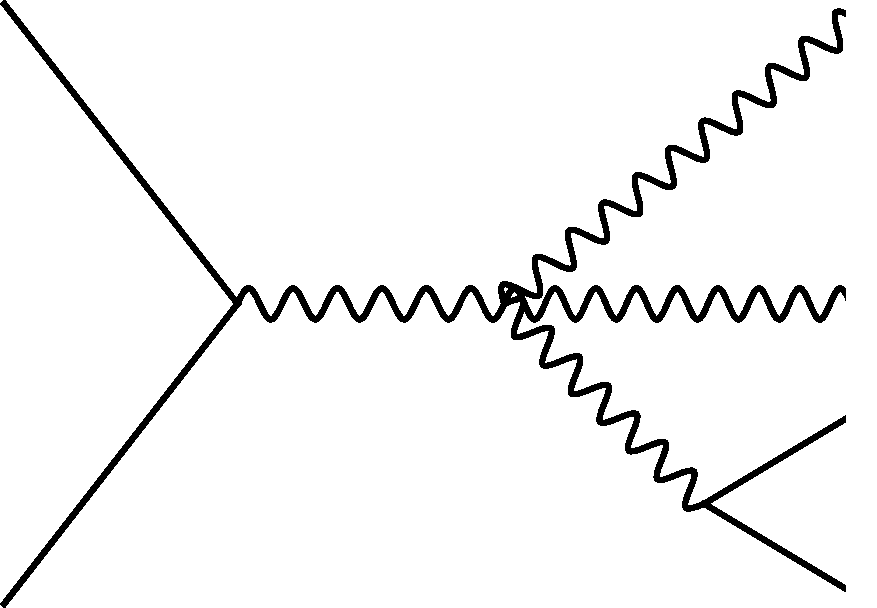
\includegraphics[width=0.3\textwidth]{figures/samples/feynEWKnonVBS4.pdf}}
\subfloat[]{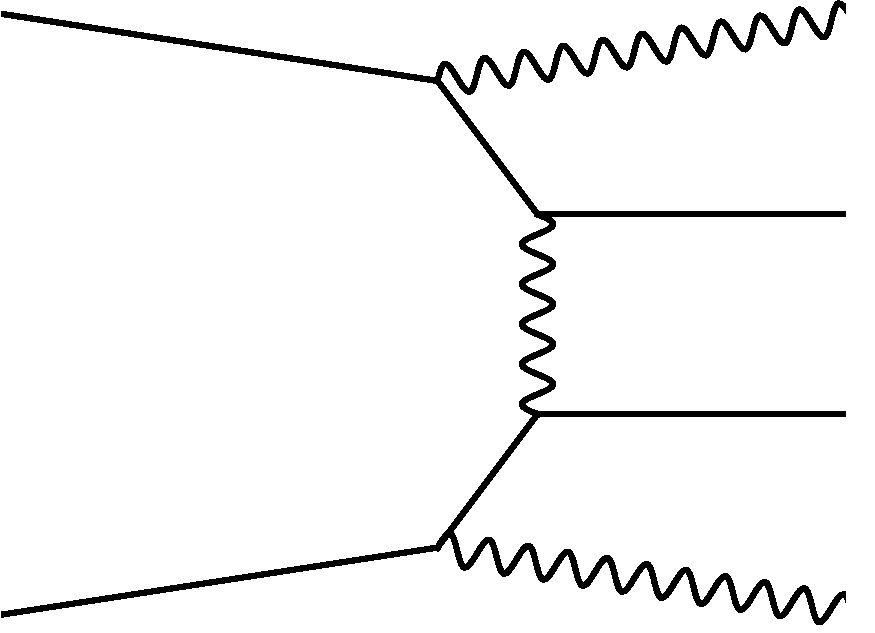
\includegraphics[width=0.3\textwidth]{figures/samples/feynEWKnonVBS5.pdf}}\\
\subfloat[]{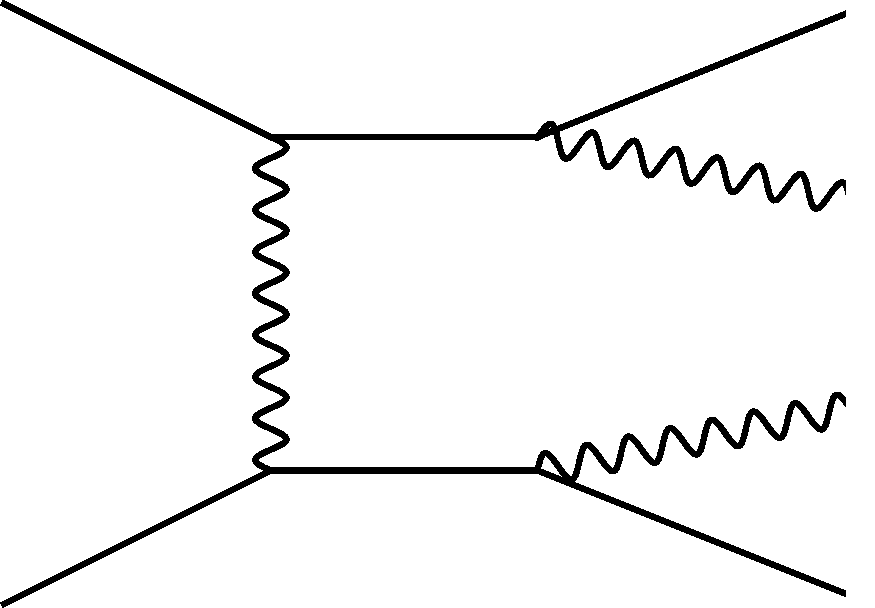
\includegraphics[width=0.3\textwidth]{figures/samples/feynEWKnonVBS6.pdf}}
\subfloat[]{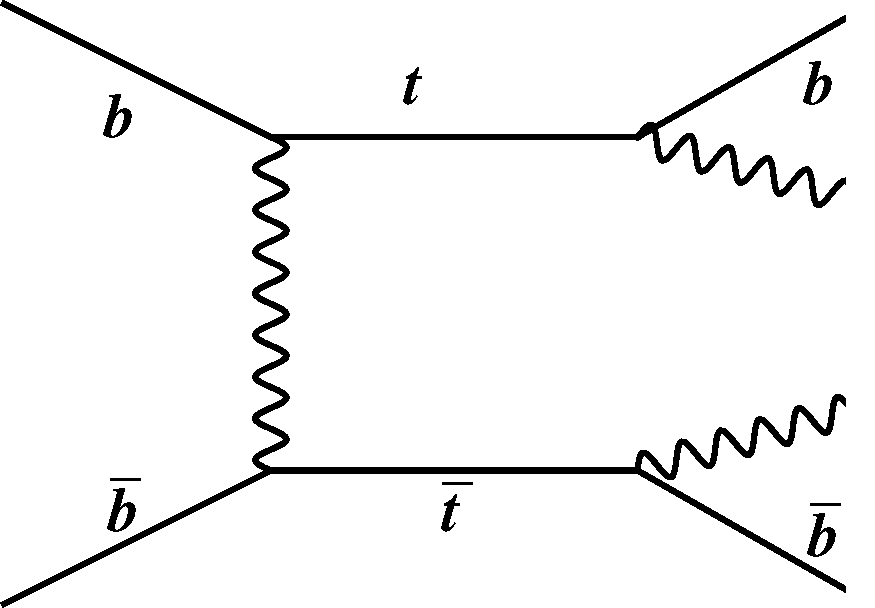
\includegraphics[width=0.3\textwidth]{figures/samples/feynEWKnonVBS1.pdf}}
\subfloat[]{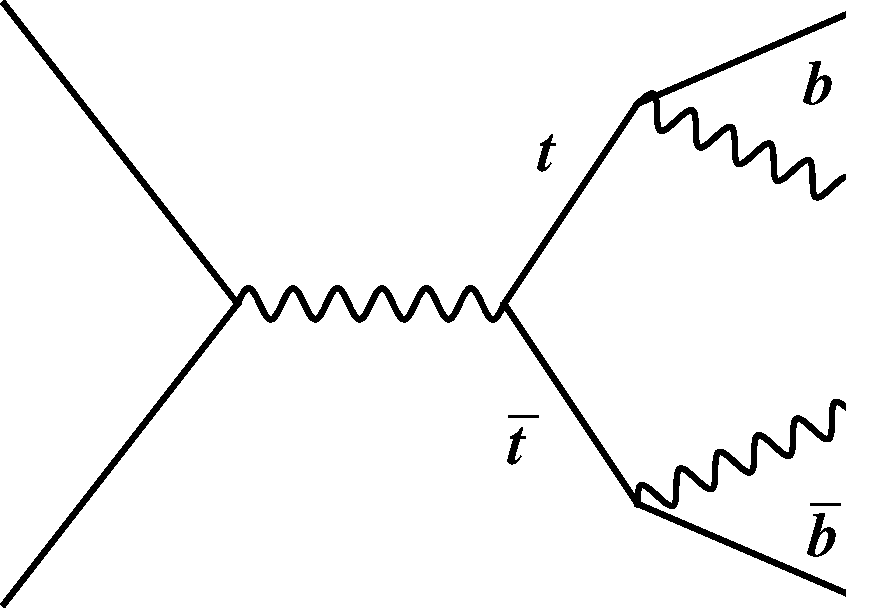
\includegraphics[width=0.3\textwidth]{figures/samples/feynEWKnonVBS2.pdf}}\\
\subfloat[]{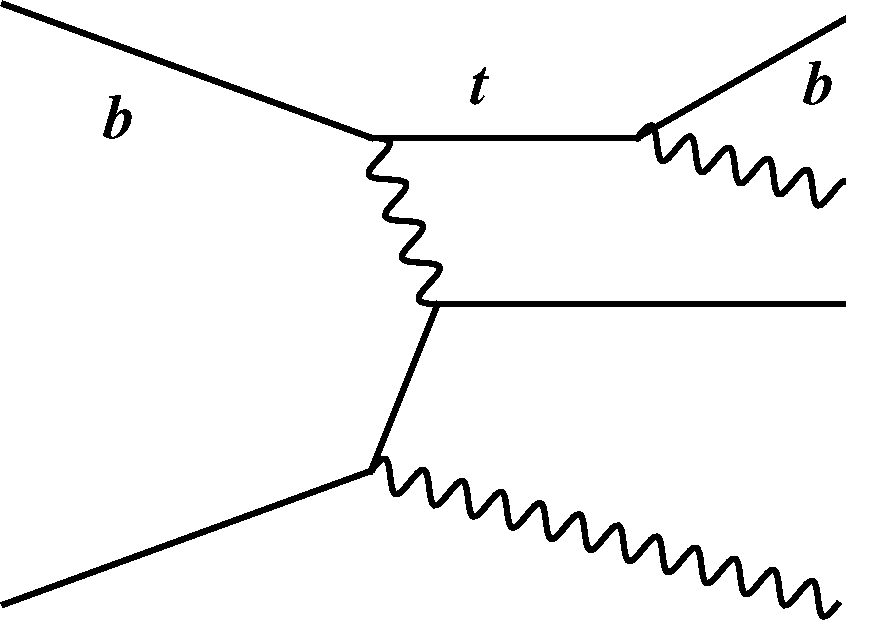
\includegraphics[width=0.3\textwidth]{figures/samples/feynEWKnonVBS7.pdf}}
\caption{
Examples of non-VBS $\mathcal{O}(\alpha_{EW}^6)$ diagrams contributin to the signal.
}
\label{fig:feynmanEWKnonVBS}
\end{center}
\end{figure}

%semileptonic and 1-lepton
Depending on the decay products of the vector bosons, VBS processes can be categorized into three types: fully leptonic, fully hadronic, and semileptonic. 
The fully leptonic VBS analysis studies final states where both vector bosons decay into leptons. 
Similarly, the fully hadronic analysis targets cases where the decay products are exclusively hadronic.
While studies of fully leptonic final states have been done, the branching ratio from double leptonic decay modes is relatively small. On the other hand, fully hadronic final states have a significantly higher branching ratio but introduce considerable background noise, making them challenging to analyze.
The semileptonic VBS analysis is looking at final states with one hadronic and one leptonic boson, offering a balanced compromise between a higher branching ratio and manageable background levels. As illustrated in Figure~\ref{fig:semi_vbs}, the two ``forward'' jets, $j_{f}$ and $j_{b}$, are high \pt jets that scatter through the coupling of the gauge bosons. These jets, pointing roughly along the beamline direction, serve as signatures of the VBS process. Further details on physics object definitions and VBS selection criteria will be discussed in Chapter~\ref{chap:objects_def} and Section~\ref{subsec:vbs_selection}.

Figure~\ref{fig:semi_vbs} also shows two jets, $j_{c}$, orginating from the hadronically decaying vector boson. 
The boson decaying leptonically can have a few conbinations of decay products. 
By counting the number of oberverable lepton(s), we have three channels in the semileptonic VBS analysis. 
Although neutrinos are technically leptons, within the context of this and similar analyses, ``lepton'' typically refers to those detectable directly by the ATLAS and CMS detectors.
Therefore, the 0-lepton channel corresponds to final states where the vector boson decays into a pair of neutrinos.
The 1-lepton channel involves one observable lepton (e.g., $e$, $\mu$) and a neutrino, while the 2-lepton channel includes final states without neutrinos. Most of the work presented in this thesis applies to all three channels but is primarily discussed from the 1-lepton channel perspective.

%Therefore, the 0-lepton channel is refering to the final states which the vector boson decay into a pair of neutrinos. The 1-lepton channel is one oberservable lepton (ie, $e$, $\mu$) and a neutrino, and the 2-lepton channel has no neutrinos. Most of the works mentioned in this thesis are generally applied to all 3 channels, but will be told from the 1-lepton channel's perspect.
%While neutrinos are leptons by definitions. In the context of this and similar analyses, lepton usually refers to the ones that can be detected directly by the ATLAS and CMS detectors. 

\begin{figure}[tbp]
\centering
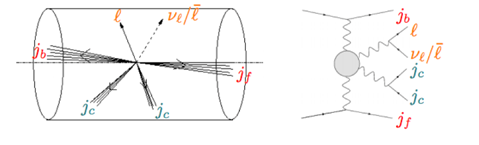
\includegraphics[width=0.75\textwidth]{figures/theory/semi_vbs.png}
\caption{
A schematic representation of a semileptonic VBS process within the detector, accompanied by the corresponding Feynman diagram.
}
\label{fig:semi_vbs}
\end{figure}

%Without the Higgs mechanism, calculations for VBS would lead to probabilities that exceed 100\% at high energies and violate unitarity. The discovery of a Higgs boson in LHC motivates further study of the mechanism of EWSB by probing the vector boson scattering (VBS) process. This process involves a quartic gauge coupling (QGC) vertex (Figure 2). The QGC is the self-coupling among four electroweak gauge bosons. The mechanism responsible for EWSB must also regularize the cross-section of SM VBS to restore unitarity above 1 TeV. Various physics models beyond the SM (BSM) predict enhancements of VBS production[6,7]. Therefore, the measurements of VBS at high energy are crucial tests of the SM and will determine whether the Higgs is entirely responsible for EWSB.

%%\begin{figure}[htbp]
%%\centering
%%\begin{subfigure}{.3\textwidth}
%%  \centering
%%\begin{tikzpicture}
%%  \begin{feynman}
%%    \vertex (a);
%%    \vertex [above left=of a] (i1) {\(V_L\)};
%%    \vertex [below left=of a] (i2) {\(V_L\)};
%%    \vertex [above right=of a] (f1) {\(V_L\)};
%%    \vertex [below right=of a] (f2) {\(V_L\)};
%%
%%    \diagram* {
%%      (i1) -- [boson] (a) -- [boson] (f1),
%%      (i2) -- [boson] (a) -- [boson] (f2),
%%    };
%%  \end{feynman}
%%\end{tikzpicture}
%%\end{subfigure}%
%%\begin{subfigure}{.3\textwidth}
%%  \centering
%%\begin{tikzpicture}
%%  \begin{feynman}
%%    \vertex (a);
%%    \vertex [above left=of a] (i1) {\(V_L\)};
%%    \vertex [below left=of a] (i2) {\(V_L\)};
%%    \vertex [right=of a] (b);
%%    \vertex [above right=of b] (f1) {\(V_L\)};
%%    \vertex [below right=of b] (f2) {\(V_L\)};
%%
%%    \diagram* {
%%      (i1) -- [boson] (a) -- [boson] (b)-- [boson] (f1),
%%      (i2) -- [boson] (a),
%%      (f2) -- [boson] (b),
%%    };
%%  \end{feynman}
%%\end{tikzpicture}
%%\end{subfigure}%
%%\begin{subfigure}{.3\textwidth}
%%  \centering
%%\begin{tikzpicture}
%%  \begin{feynman}
%%    \vertex (a);
%%    \vertex [above left=of a] (i1) {\(V_L\)};
%%    \vertex [above right=of a] (i2) {\(V_L\)};
%%    \vertex [below=of a] (b);
%%    \vertex [below left=of b] (f1) {\(V_L\)};
%%    \vertex [below right=of b] (f2) {\(V_L\)};
%%
%%    \diagram* {
%%      (i1) -- [boson] (a) -- [boson] (b)-- [boson] (f1),
%%      (i2) -- [boson] (a),
%%      (f2) -- [boson] (b),
%%    };
%%  \end{feynman}
%%\end{tikzpicture}
%%\end{subfigure}
%%
%%\vspace{2cm}
%%\begin{subfigure}{.3\textwidth}
%%  \centering
%%\begin{tikzpicture}
%%  \begin{feynman}
%%    \vertex (a);
%%    \vertex [above left=of a] (i1) {\(V_L\)};
%%    \vertex [below left=of a] (i2) {\(V_L\)};
%%    \vertex [right=of a] (b);
%%    \vertex [above right=of b] (f1) {\(V_L\)};
%%    \vertex [below right=of b] (f2) {\(V_L\)};
%%
%%    \diagram* {
%%      (i1) -- [boson] (a) -- [scalar, edge label=\(H\)] (b)-- [boson] (f1),
%%      (i2) -- [boson] (a),
%%      (f2) -- [boson] (b),
%%    };
%%  \end{feynman}
%%\end{tikzpicture}
%%\end{subfigure}
%%\begin{subfigure}{.3\textwidth}
%%  \centering
%%\begin{tikzpicture}
%%  \begin{feynman}
%%    \vertex (a);
%%    \vertex [above left=of a] (i1) {\(V_L\)};
%%    \vertex [above right=of a] (i2) {\(V_L\)};
%%    \vertex [below=of a] (b);
%%    \vertex [below left=of b] (f1) {\(V_L\)};
%%    \vertex [below right=of b] (f2) {\(V_L\)};
%%
%%    \diagram* {
%%      (i1) -- [boson] (a) -- [scalar, edge label=\(H\)] (b)-- [boson] (f1),
%%      (i2) -- [boson] (a),
%%      (f2) -- [boson] (b),
%%    };
%%  \end{feynman}
%%\end{tikzpicture}
%%\end{subfigure}
%%\caption{The tree-level Feynman diagrams contributing to VBS process.}
%%\label{fig:feynman_diagrams}
%%\end{figure}




\clearpage
\section{Beyond the Standard Model}
%aQGCs
Despite intensive searches, experiments at the LHC have not yet observed new physics phenomena beyond those predicted by the Standard Model of particle physics.
After the discovery of the Higgs boson, a significant number of analyses have been dedicated to searching for traces of new particles. In the meantime, we also explore the possibility of Beyond the Standard Model (BSM) interactions involving known Standard Model particles, such as the Higgs, $W$, and $Z$ bosons. Any potential new physics related to EWSB could thus modify the interactions of these particles.
In our case where no new physics has yet been found, the Standard Model can be considered as a low-energy approximation of a more comprehensive theory.
This perspective allows us to describe potential BSM phenomena through an Effective Field Theory (EFT)  approach~\cite{Weinberg:1978kz}~\cite{RevModPhys.52.515}.

\subsection{Anomalous Quartic Gauge Couplings}
\label{Anomalous_Quartic_Gauge_Couplings}

The concept of anomalous couplings among electroweak vector bosons existed before the Higgs boson was discovered~\cite{GaemersGounaris1979}. Even then, it was widely believed that EWSB governed the electroweak interactions, ensuring they remained consistent without violating any unitarity constraints.
Given the discovery of the Higgs boson and the solid foundation of the $\mathrm{SU}(3)_C \otimes \mathrm{SU}(2)_L \otimes \mathrm{U}(1)_Y$ gauge symmetry, employing an EFT approach has emerged as a compelling method for predicting and analyzing precise measurements of electroweak processes, including any deviations from expected results.

The EFT framework offers a streamlined and versatile way to explore anomalous couplings without being tied to any specific model~\cite{Degrande_2013}. This includes both anomalous triple gauge couplings (aTGCs) and anomalous quartic gauge couplings (aQGCs). Although aTGCs remain a significant area of interest, our focus here will be aQGCs. aQGCs are particularly intriguing because they can be investigated through VBS, providing a clear pathway for probing these potential deviations.

Assuming that new physics emerges only at energies above the scale $\Lambda$, we can describe any phenomena beyond the Standard Model (including anomalous gauge couplings) using an effective Lagrangian:
\begin{equation}
\mathcal{L}_{\text{eff}} = \mathcal{L}_{\text{SM}} + \sum_i \frac{c^{(6)}_i}{\Lambda^2} \mathcal{O}^{(6)}_i + \sum_j \frac{c^{(8)}_j}{\Lambda^4} \mathcal{O}^{(8)}_j + \ldots
\end{equation} 
where $\mathcal{L}_{\text{SM}}$ is the Standard Model Lagrangian, $\mathcal{O}_i$ are the higher-dimensional operators of dimension $d_i$, $c_i$ are the Wilson coefficients.
In the effective Lagrangian, we include only even-dimensional operators because odd-dimensional operators would violate lepton and/or baryon number conservation~\cite{Degrande_2013}. 
The dimension-6 (D-6) terms, $\frac{c^{(6)}_i}{\Lambda^2} \mathcal{O}^{(6)}_i$, are often associated with aTGCs. 
The dimension-8 (D-8) terms, $\frac{c^{(8)}_j}{\Lambda^4} \mathcal{O}^{(8)}_j$, are typically associated with aQGCs, introducing or modifying interactions involving four gauge bosons.
Although both D-6 and D-8 operators can contribute to the VBS processes, the D-6 operators have been tightly constrained to values around zero by previous diboson measurements. Therefore, we will focus our discussion on the D-8 operators here.


Building on the EFT approach to model the effects of possible aQGCs, we adopt the Eboli model, which introduces 21 new D-8 operators adhering to the SM $SU(2)\times U(1)_Y$ gauge symmetry~\cite{eboli2006p}.
These operators can be classified into three categories: scalar, tensor, and mixed types. A list of these operators is provided at the end of this section.
As shown in Table~\ref{table:eboli_op}, the semileptonic VBS stands out as an exceptional process capable of testing nineteen D-8 operators concurrently, with final states that involved $WW$, $WZ$, and $ZZ$ boson pairs.

\begin{table}[h!]
	\centering
	\begin{tabular}{|c|c|c|c||c|c|c|c|c|c|}
		\hline
		& WWWW & WWZZ & ZZZZ & WW$\gamma$Z & WW$\gamma\gamma$ & ZZZ$\gamma$ & ZZ$\gamma\gamma$ & Z$\gamma\gamma\gamma$ & $\gamma\gamma\gamma\gamma$ \\ \hline
		$\mathcal{L}_{S0,2}, \mathcal{L}_{S1}$ & X & X & X & — & — & — & — & — & — \\ \hline
		$\mathcal{L}_{M0}, \mathcal{L}_{M1}, \mathcal{L}_{M6}, \mathcal{L}_{M7}$ & X & X & X & X & X & X & X & — & — \\ \hline
		$\mathcal{L}_{M2}, \mathcal{L}_{M3}, \mathcal{L}_{M4}, \mathcal{L}_{M5}$ & — & X & X & X & X & X & X & — & — \\ \hline
		$\mathcal{L}_{T0}, \mathcal{L}_{T1}, \mathcal{L}_{T2}$ & X & X & X & X & X & X & X & X & X \\ \hline
		$\mathcal{L}_{T5}, \mathcal{L}_{T6}, \mathcal{L}_{T7}$ & — & X & X & X & X & X & X & X & X \\ \hline
		$\mathcal{L}_{T8}, \mathcal{L}_{T9}$ & — & — & X & — & — & — & X & X & X \\ \hline
	\end{tabular}
	\caption{Correspondences between the vertices and operators. The ``X'' marks indicate the quartic gauge vertices that can be modified by the specified D-8 operators.}
	\label{table:eboli_op}
\end{table}


%%%%%%%%%%%%%%%%%%%%%%%%%%%%%%%%%
The following are the three classes of D-8 operators in the Eboli model~\cite{eboli2006p}.

The scalar operators containing just covariant derivatives of the Higgs field, $D_\mu\Phi$:
\begin{eqnarray}
  {\cal L}_{S0,2} &=& \left [ \left ( D_\mu \Phi \right)^\dagger
 D_\nu \Phi \right ] \times
\left [ \left ( D^\mu \Phi \right)^\dagger
D^\nu \Phi \right ]
\\
  {\cal L}_{S1} &=& \left [ \left ( D_\mu \Phi \right)^\dagger
 D^\mu \Phi  \right ] \times
\left [ \left ( D_\nu \Phi \right)^\dagger
D^\nu \Phi \right ]
\end{eqnarray}
Here, the operators $\mathcal{L}_{S0}$ and $\mathcal{L}_{S2}$ are Hermitian conjugates, and can be treated as the same operator in practice.

The tensor operators containing just the field strength tensor:
\begin{eqnarray}
 {\cal L}_{T,0} &=&   \hbox{Tr}\left [ \hat{W}_{\mu\nu} \hat{W}^{\mu\nu} \right ]
\times   \hbox{Tr}\left [ \hat{W}_{\alpha\beta} \hat{W}^{\alpha\beta} \right ]
\\
 {\cal L}_{T,1} &=&   \hbox{Tr}\left [ \hat{W}_{\alpha\nu} \hat{W}^{\mu\beta} \right ]
\times   \hbox{Tr}\left [ \hat{W}_{\mu\beta} \hat{W}^{\alpha\nu} \right ]
\\
 {\cal L}_{T,2} &=&   \hbox{Tr}\left [ \hat{W}_{\alpha\mu} \hat{W}^{\mu\beta} \right ]
\times   \hbox{Tr}\left [ \hat{W}_{\beta\nu} \hat{W}^{\nu\alpha} \right ]
\\
 {\cal L}_{T,3} &=&   \hbox{Tr}\left [ \hat{W}_{\alpha\mu}
   \hat{W}^{\mu\beta}  \hat{W}^{\nu\alpha} \right ]
\times   B_{\beta\nu}
\\
 {\cal L}_{T,4} &=&   \hbox{Tr}\left [ \hat{W}_{\alpha\mu}
   \hat{W}^{\alpha\mu}  \hat{W}^{\beta\nu} \right ]
\times   B_{\beta\nu}
\\
 {\cal L}_{T,5} &=&   \hbox{Tr}\left [ \hat{W}_{\mu\nu} \hat{W}^{\mu\nu} \right ]
\times   B_{\alpha\beta} B^{\alpha\beta}
\\
 {\cal L}_{T,6} &=&   \hbox{Tr}\left [ \hat{W}_{\alpha\nu} \hat{W}^{\mu\beta} \right ]
\times   B_{\mu\beta} B^{\alpha\nu} 
\\
 {\cal L}_{T,7} &=&   \hbox{Tr}\left [ \hat{W}_{\alpha\mu} \hat{W}^{\mu\beta} \right ]
\times   B_{\beta\nu} B^{\nu\alpha} 
\\
 {\cal L}_{T,8} &=&   B_{\mu\nu} B^{\mu\nu}  B_{\alpha\beta} B^{\alpha\beta}
\\
 {\cal L}_{T,9} &=&  B_{\alpha\mu} B^{\mu\beta}   B_{\beta\nu} B^{\nu\alpha} 
\end{eqnarray}

The mixed operators containing $D_\mu\Phi$ and field strength:
\begin{eqnarray}
 {\cal L}_{M,0} &=&   \hbox{Tr}\left [ \hat{W}_{\mu\nu} \hat{W}^{\mu\nu} \right ]
\times  \left [ \left ( D_\beta \Phi \right)^\dagger
D^\beta \Phi \right ]
\\
 {\cal L}_{M,1} &=&   \hbox{Tr}\left [ \hat{W}_{\mu\nu} \hat{W}^{\nu\beta} \right ]
\times  \left [ \left ( D_\beta \Phi \right)^\dagger
D^\mu \Phi \right ]
\\
 {\cal L}_{M,2} &=&   \left [ B_{\mu\nu} B^{\mu\nu} \right ]
\times  \left [ \left ( D_\beta \Phi \right)^\dagger
D^\beta \Phi \right ]
\\
 {\cal L}_{M,3} &=&   \left [ B_{\mu\nu} B^{\nu\beta} \right ]
\times  \left [ \left ( D_\beta \Phi \right)^\dagger
D^\mu \Phi \right ]
\\
  {\cal L}_{M,4} &=& \left [ \left ( D_\mu \Phi \right)^\dagger \hat{W}_{\beta\nu}
 D^\mu \Phi  \right ] \times B^{\beta\nu}
\\
  {\cal L}_{M,5} &=& \left [ \left ( D_\mu \Phi \right)^\dagger \hat{W}_{\beta\nu}
 D^\nu \Phi  \right ] \times B^{\beta\mu}
\\
  {\cal L}_{M,6} &=& \left [ \left ( D_\mu \Phi \right)^\dagger \hat{W}_{\beta\nu}
\hat{W}^{\beta\nu} D^\mu \Phi  \right ] 
\\
  {\cal L}_{M,7} &=& \left [ \left ( D_\mu \Phi \right)^\dagger \hat{W}_{\beta\nu}
\hat{W}^{\beta\mu} D^\nu \Phi  \right ] 
\end{eqnarray}




%\section{Standard Model}
%\section{The Higgs Mechanism}
%\section{Vector Boson Scattering}
%\section{Beyond the Standard Model}
%\subsection{aQGC}

\chapter{Experimental Apparatus}
%Experimental Apparatus
\label{ch:Experimental_Apparatus}

\section{The LHC}
\label{the_lhc}

The Large Hadron Collider (LHC)~\cite{Bruning:782076} at CERN is currently the world's largest and most powerful hadron accelerator and collider.
It is located in a circular tunnel roughly 100 m beneath the borders of Switzerland and France. The tunnel is about 27 kilometers long and was initially built for the Large Electron-Positron Collider (LEP), which operated from 1989 to 2000. Construction of the LHC began in 1998 and was completed in 2008. There are eight Interaction Points (IP) where particle beams can collide, four located in caverns, each housing one of the four experiments of the LHC: ATLAS~\cite{TheATLASCollaboration_2008}, CMS~\cite{TheCMSCollaboration_2008}, LHCb~\cite{TheLHCbCollaboration_2008}, and ALICE~\cite{TheALICECollaboration_2008}.
The ATLAS and CMS experiments search for the same types of collision events and are used to cross-check one another’s results.

The LHC was designed to collide proton beams at a center-of-mass energy of 14 TeV and a maximum instantaneous luminosity of 
$10 \, \mathrm{nb}^{-1} \, \mathrm{s}^{-1} (10^{34} \, \mathrm{cm}^{-2}\mathrm{s}^{-1})$~\cite{LyndonEvans_2008}.
The proton beams are guided by a sophisticated system of superconducting magnets. This system includes 1,232 dipole magnets with an \SI{8.3}{\tesla} strength for bending the beams and 392 main quadrupole magnets with a \SI{7.5}{\tesla} strength for focusing the beams~\cite{1288863}~\cite{1324760}.
To sustain their superconducting state and counteract external sources of heat, the magnets are immersed in a liquid helium bath at 1.9 K within a vacuum-sealed inner vessel, as seen in Figure~\ref{fig:lhc_dipole}.

\begin{figure}[ht]
    \centering
    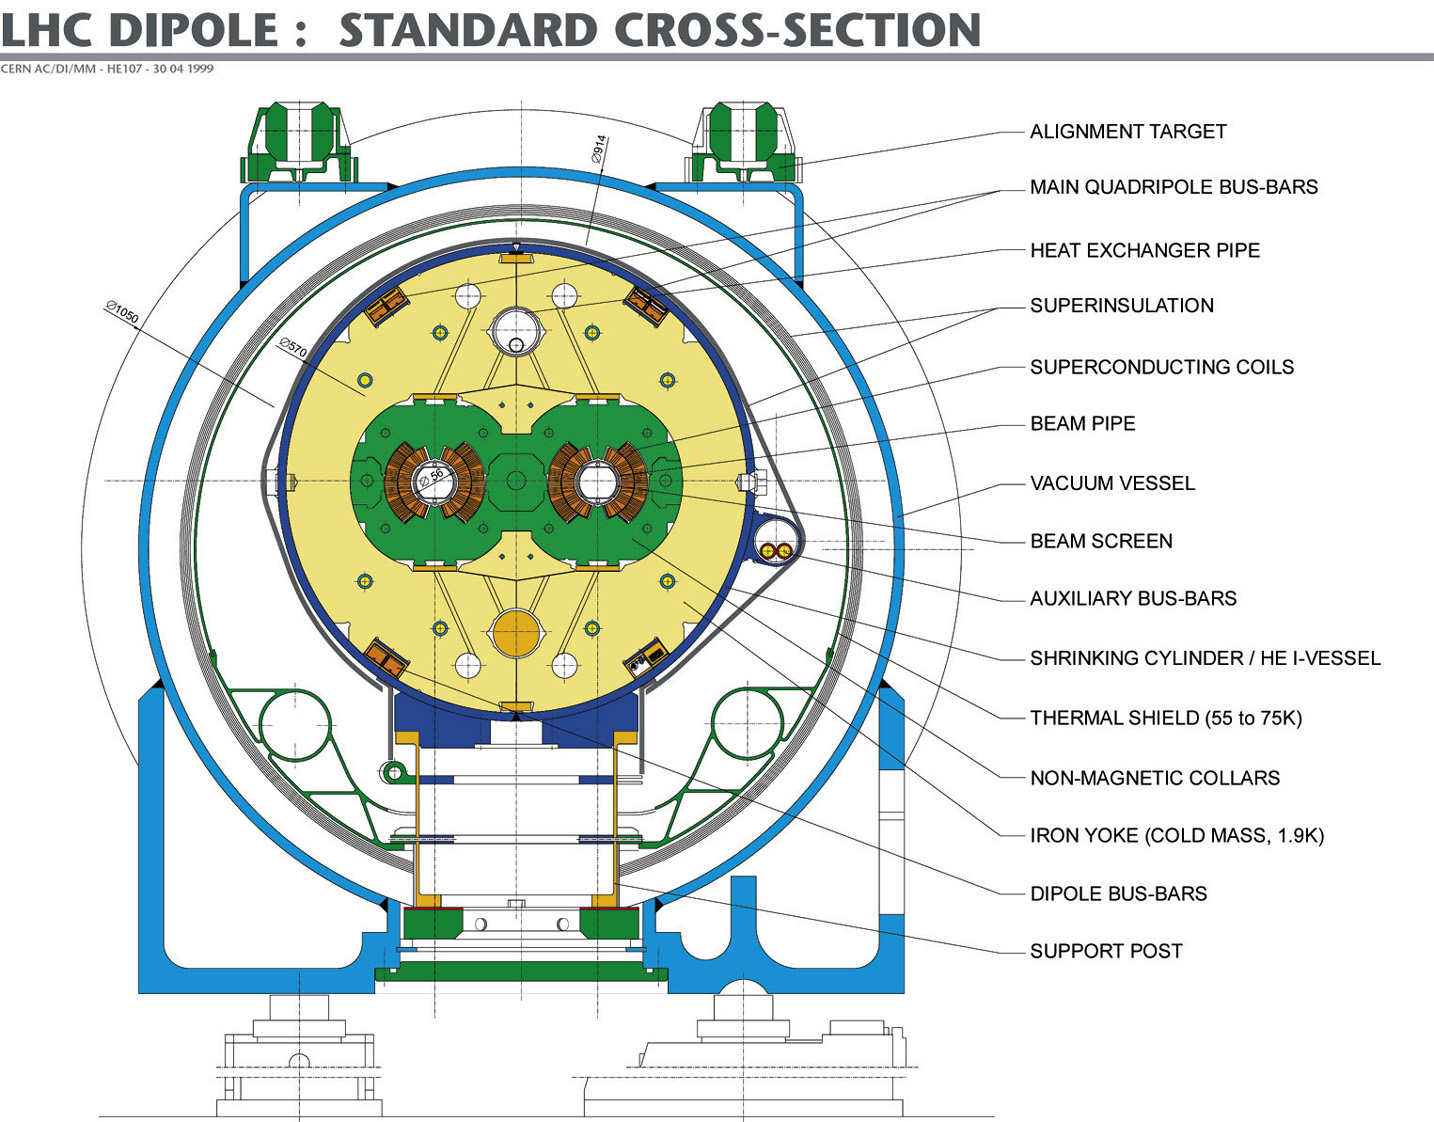
\includegraphics[width=0.75\textwidth]{figures/LHC/LHC_dipole.jpg}
    \caption[]{The cross-section of an LHC dipole magnet with vacuum chamber~\cite{Team:40524}.}
    \label{fig:lhc_dipole}
\end{figure}

Before entering the LHC, the proton beams went through a sequence of accelerators, as shown in Figure~\ref{fig:cern_complex}, which gradually increased the beams' energy. 
A single bottle of Hydrogen gas serves as the sole proton source for the whole LHC. 
At the LINAC2 linear accelerator site, the hydrogen gas is introduced into the duoplasmatron, which ionizes the gas to create a plasma of electrons and hydrogen ions~\cite{Burnet:1359959}. The plasma is then manipulated by strong electrical and magnetic fields, which separate and accelerate the protons out of the duoplasmatron and into the accelerator. 
The protons enter the LINAC2 at about 90 keV and are accelerated to 50 MeV before arriving in the Booster.
The Booster is a (relatively) small synchrotron, followed by the Proton Synchrotron (PS) and Super Proton Synchrotron (SPS). The proton beam is accelerated gradually at each stage and split before entering the LHC as two countercirculating beams. The details of this process are summarized in Table~\ref{table:accelerators}.

Within the synchrotrons, the proton beam is repeatedly passed through the radiofrequency (RF) cavities, metallic chambers containing an electromagnetic field.
This process accelerates the protons and organizes them into bunches with 25 ns spacing.
Once the proton bunches circulate in the LHC, they are further accelerated while maintaining a 25 ns spacing. The beams can circulate stably in the LHC for many hours and only need to be refilled if the beam is dumped~\cite{LyndonEvans_2008}.

\begin{figure}[ht]
    \centering
    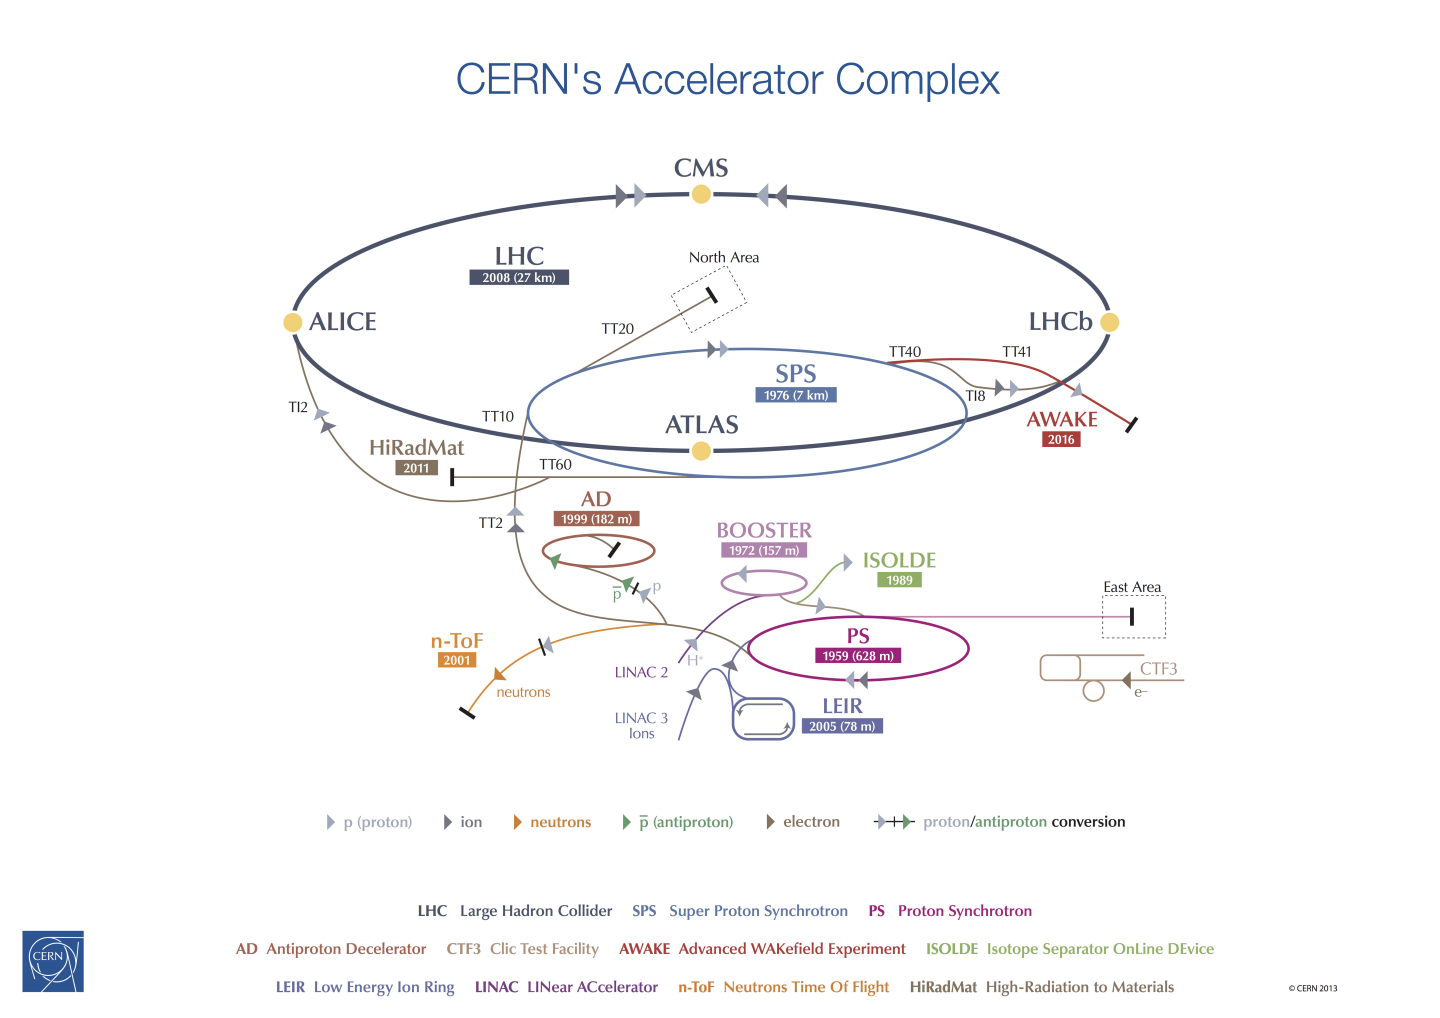
\includegraphics[width=0.8\textwidth]{figures/LHC/CERN_ComplexL.jpg}
    \caption[]{The CERN accelerator complex~\cite{Haffner:1621894}. The LHC proton injector chain is denoted by the light grey arrows.}
    \label{fig:cern_complex}
\end{figure}

\begin{table}[ht]
\centering
\begin{adjustbox}{width=0.95\textwidth}
\begin{tabular}{|l|l|l|l|}
\hline
\textbf{Accelerator Name} & \textbf{Type} & \textbf{Dimensions/Circumference} & \textbf{Exit/Final Energy} \\ \hline
LINAC2 & Linear Accelerator & - & 50 MeV \\ \hline
Booster & Synchrotron & 157 m & 1.4 GeV \\ \hline
Proton Synchrotron (PS) & Synchrotron & 628 m & 26 GeV \\ \hline
Super Proton Synchrotron (SPS) & Synchrotron & 7 km & 450 GeV \\ \hline
Large Hadron Collider (LHC) & Synchrotron & 27 km & 6.5 TeV (per beam) \\ \hline
\end{tabular}
\end{adjustbox}
\caption{Summary of CERN's Accelerator Chain Leading to the LHC}
\label{table:accelerators}
\end{table}

\clearpage
\section{The ATLAS Detector}
The ATLAS (A Toroidal LHC ApparatuS) detector~\cite{TheATLASCollaboration_2008} is a general purpose detector designed to search for all types of interesting physics events at a high luminosity. The ATLAS experiment is one of the four main LHC experiments. The ATLAS detector is located in the experiment cavern at Point 1 of the LHC at the same depth as the tunnel, roughly 100 m underground.

The detector is a large cylindrical shape, 44 m long and 25 m in diameter, and weighs approximately 7000 tonnes. Figure~\ref{fig:atlas_scale} shows the sub-detector systems of ATLAS and the relative human scale. The beam pipe is encased by the Inner Detector (ID), which in turn is surrounded by the calorimeters, and these are all nested inside the muon spectrometer (see Figure \ref{fig:atlas_cross}).
The LHC coordinate system is illustrated as a rectangular coordinate system in Figure~\ref{fig:atlas_coordinate}

\begin{figure}[ht]
    \centering
    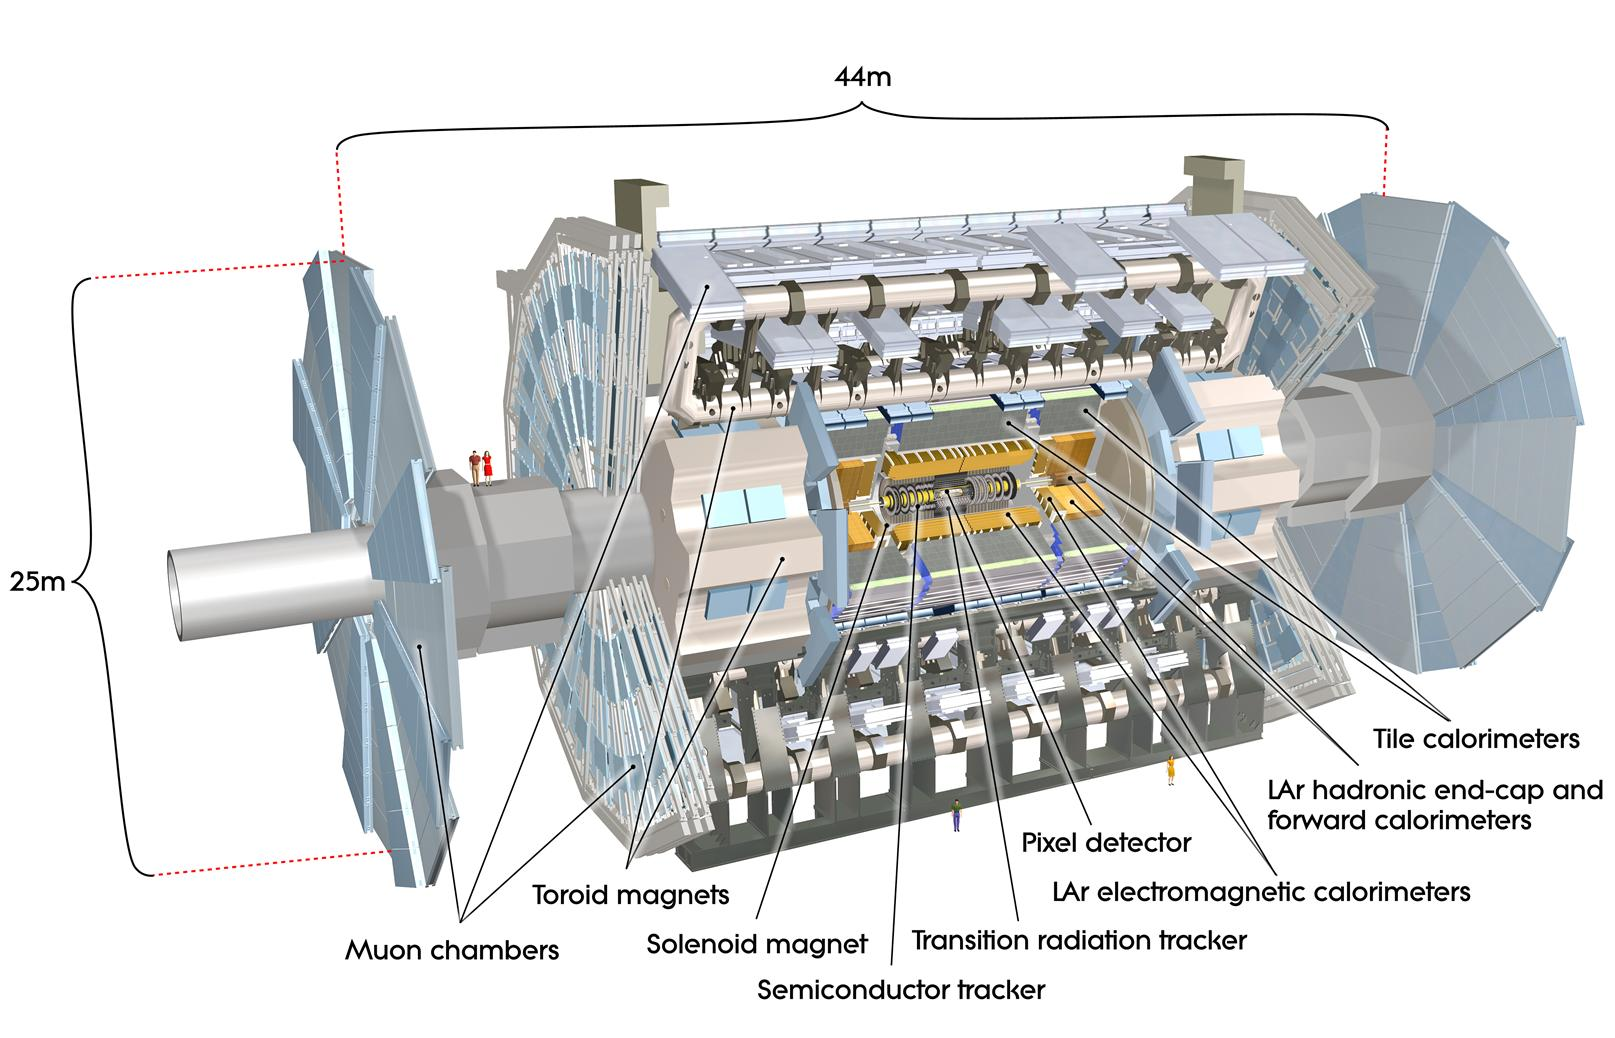
\includegraphics[width=0.85\textwidth]{figures/LHC/atlas_scale.jpg}
    \caption[]{ATLAS detector with human models included for scale~\cite{Pequenao:1095924}.}
    \label{fig:atlas_scale}
\end{figure}

\begin{figure}[ht]
    \centering
    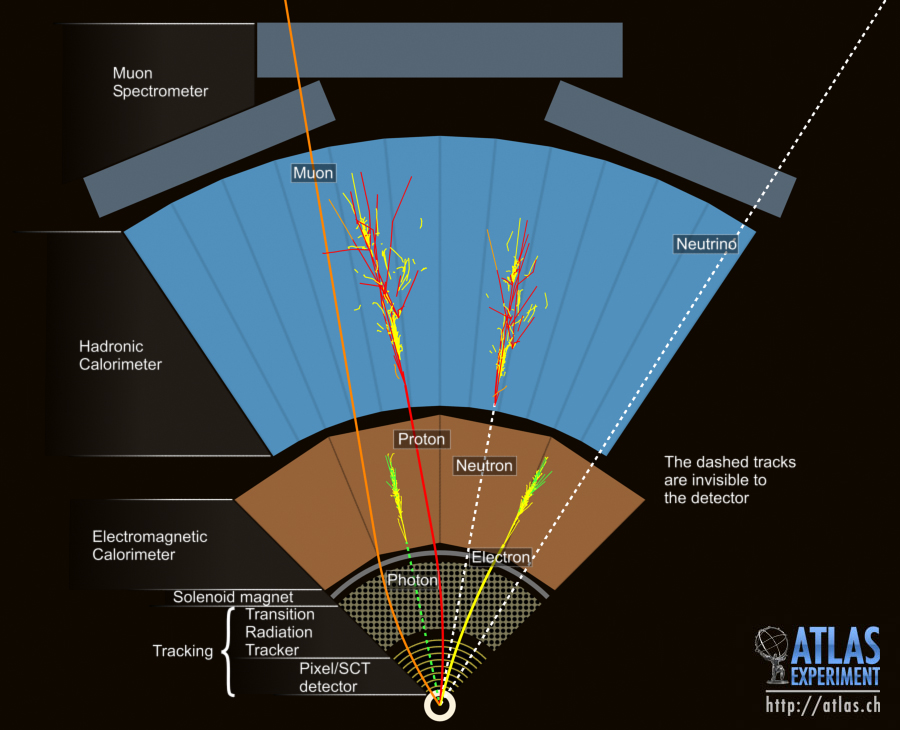
\includegraphics[width=0.75\textwidth]{figures/LHC/atlas_cross.jpg}
    \caption[]{The inner layers of ATLAS, depicted in a cross-sectional view along the x-y plane~\cite{Pequenao:1095924}.}
    \label{fig:atlas_cross}
\end{figure}

\begin{figure}[ht]
\centering
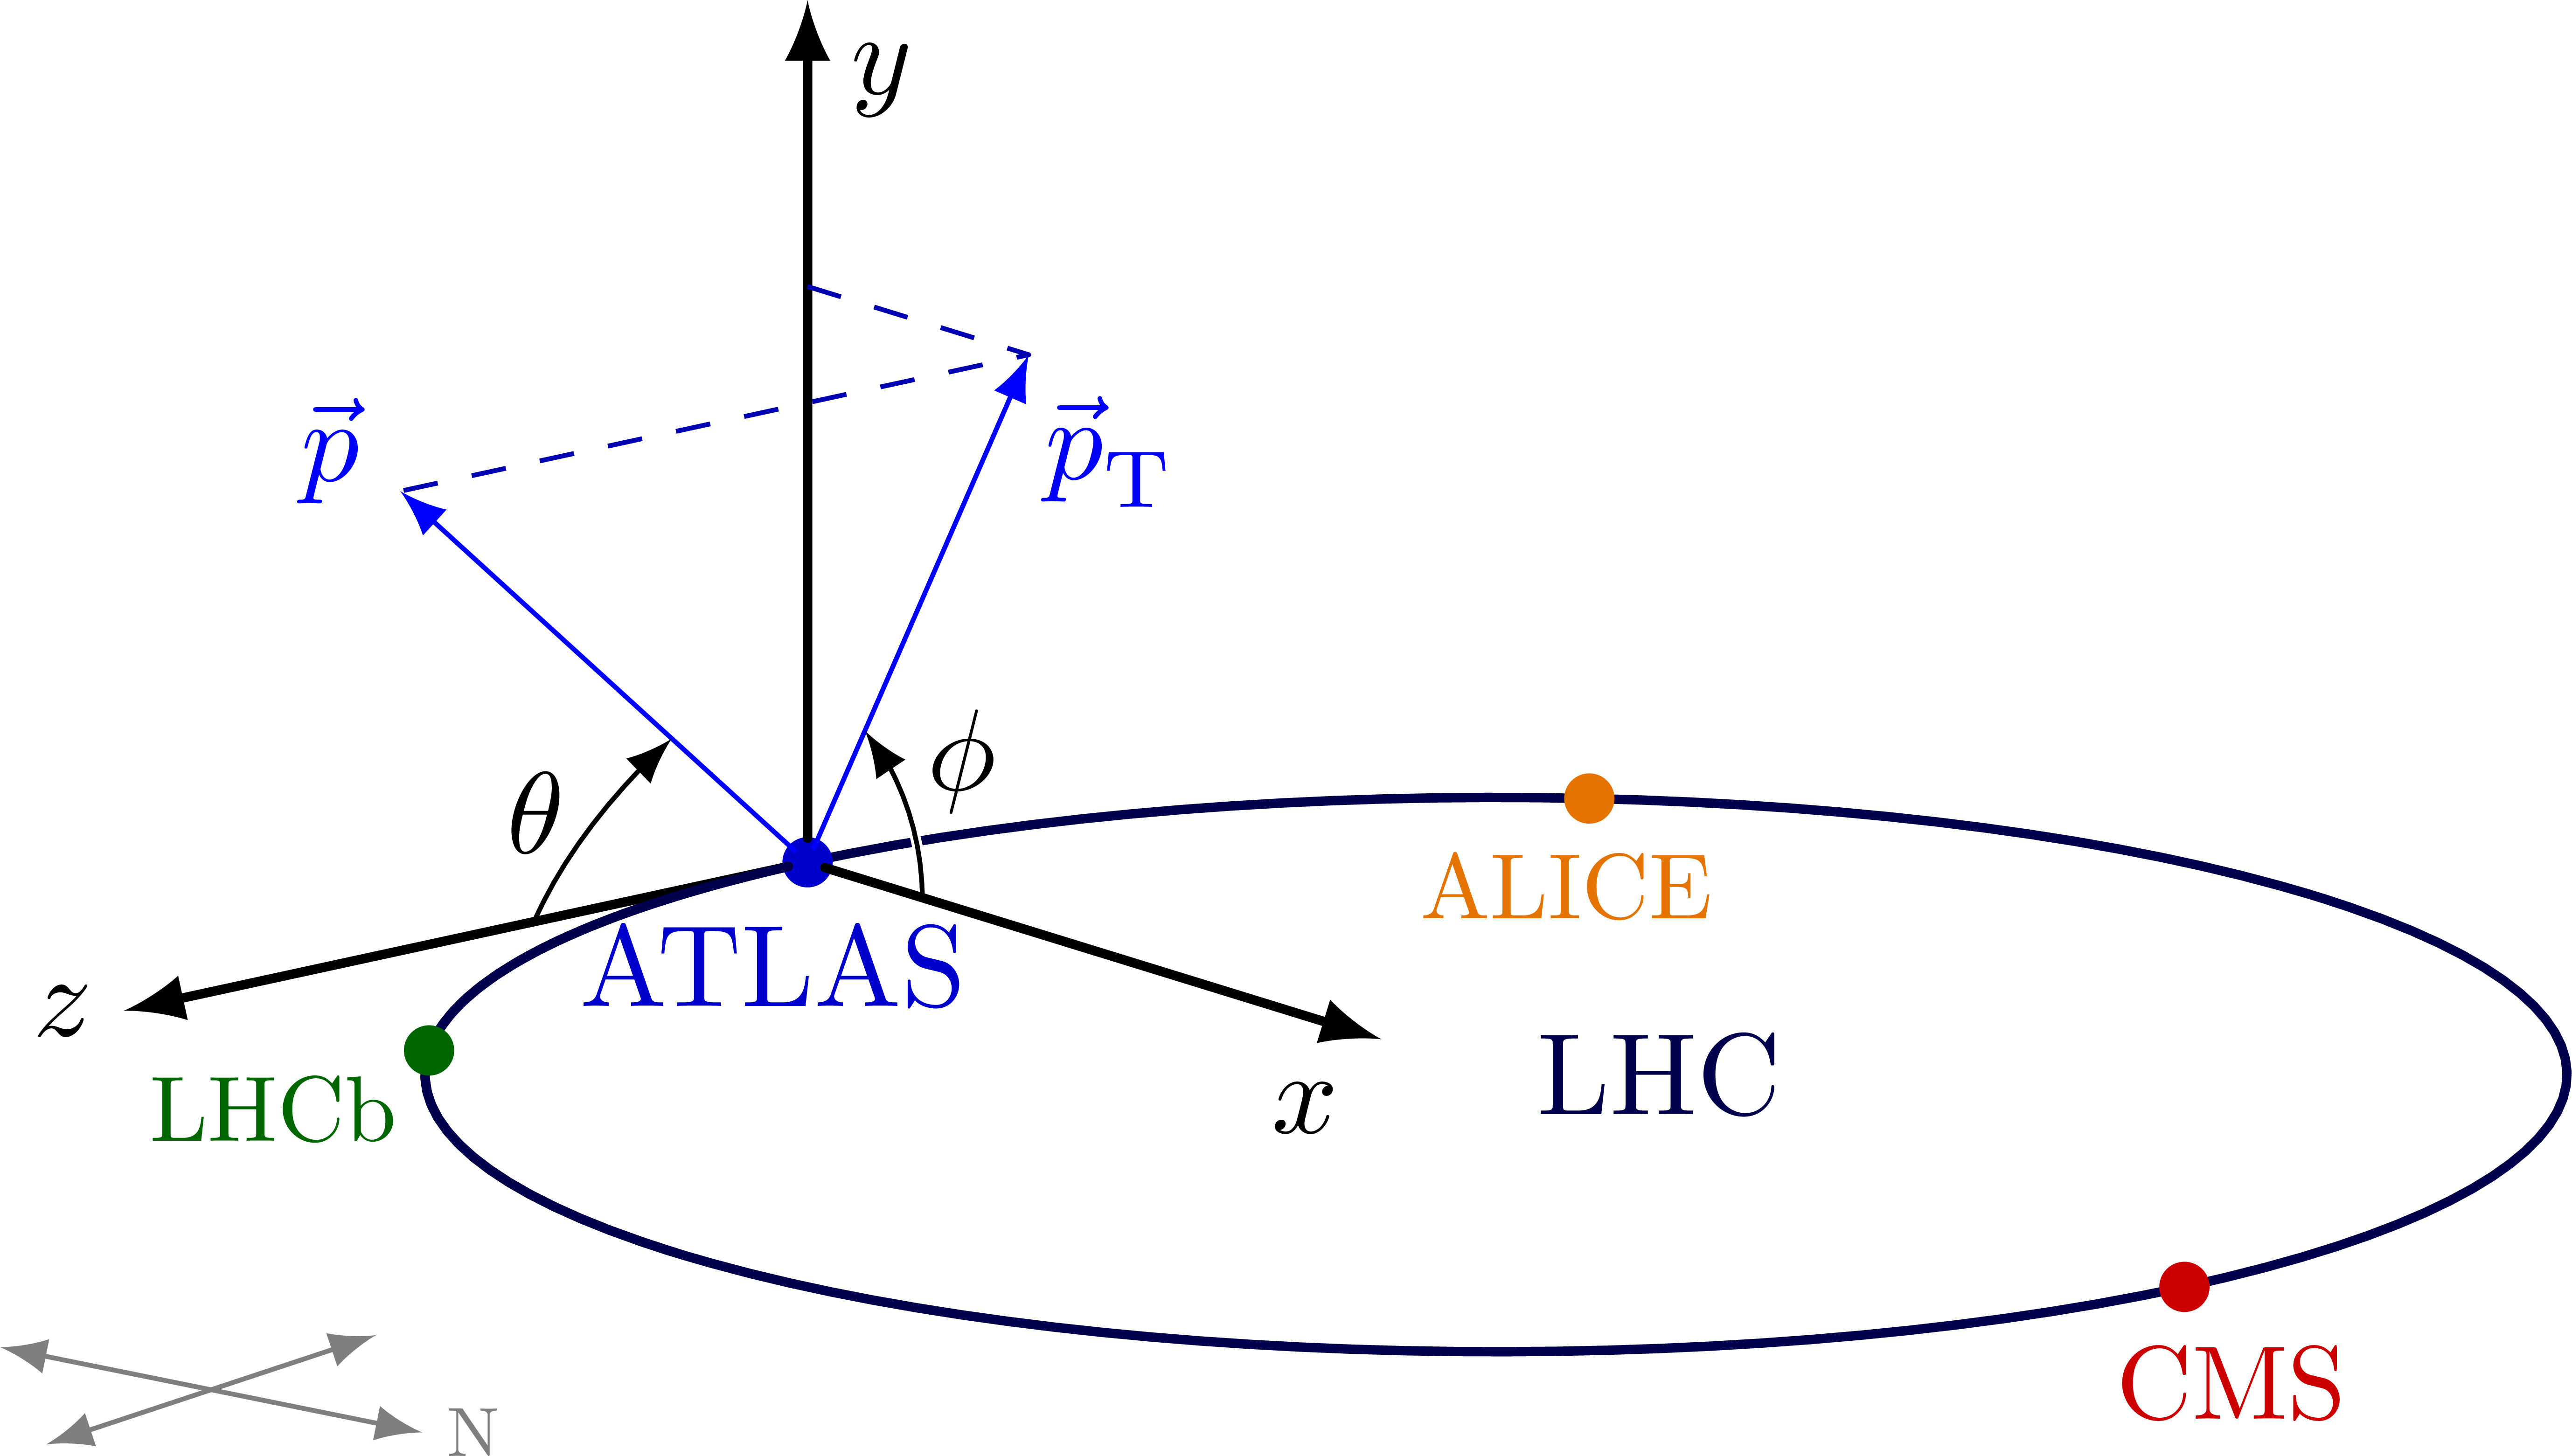
\includegraphics[width=0.75\textwidth]{figures/LHC/axis3D_CMS-003.png}
\caption[The LHC coordinate system]{The LHC coordinate system as seen from the ATLAS detector~\cite{neutelings2023lhc}.}
\label{fig:atlas_coordinate}
\end{figure}

In the transverse plane of this right-handed coordinate system, positive x points toward the center of the LHC ring, and positive y points toward the sky.
The beam pipe defines the orientation of the z-axis, with the positive direction going counterclockwise around the LHC ring.
While the LHC coordinate system is Cartesian, the coordinate system preferred for describing LHC events, particularly in the ATLAS experiment, utilizes a particle's transverse momentum ($p_T$), pseudorapidity ($\eta$), and azimuthal angle ($\phi$). The polar angle ($\theta$) is defined relative to the beam axis, whereas the azimuthal angle ($\phi$) is measured in the plane perpendicular to the beam.
In practice, pseudorapidity is preferred over the polar angle. It is defined as
\begin{equation}
    \eta = -\ln \left( \tan \frac{\theta}{2} \right)
\end{equation}
and is a good approximation of the rapidity of a particle in the high-energy regime, which is a measurement of the particle's velocity along the beam axis, given by
\begin{equation}
    y = \frac{1}{2} \ln \left( \frac{E + p_z}{E - p_z} \right).
\end{equation}

While neither the rapidity nor the pseudorapidity are Lorentz invariants, the rapidity difference between the two particles is invariant under Lorentz boosts along the direction of motion. Similarly, the difference in pseudorapidities is approximately invariant under such boosts, especially for highly relativistic particles in LHC/ATLAS events.

%%%ID
\subsection{The Inner Detector}
Located inside the solenoid magnet, the Inner Detector (ID)~\cite{ATLAS:1998yql} consists of three subsystems designed to detect charged particles, covering a pseudorapidity range of \(|\eta| < 2.5\). As seen in Figure~\ref{fig:id_layout}, these subsystems are described from the innermost to the outermost as follows.

\begin{figure}[ht]
    \centering
    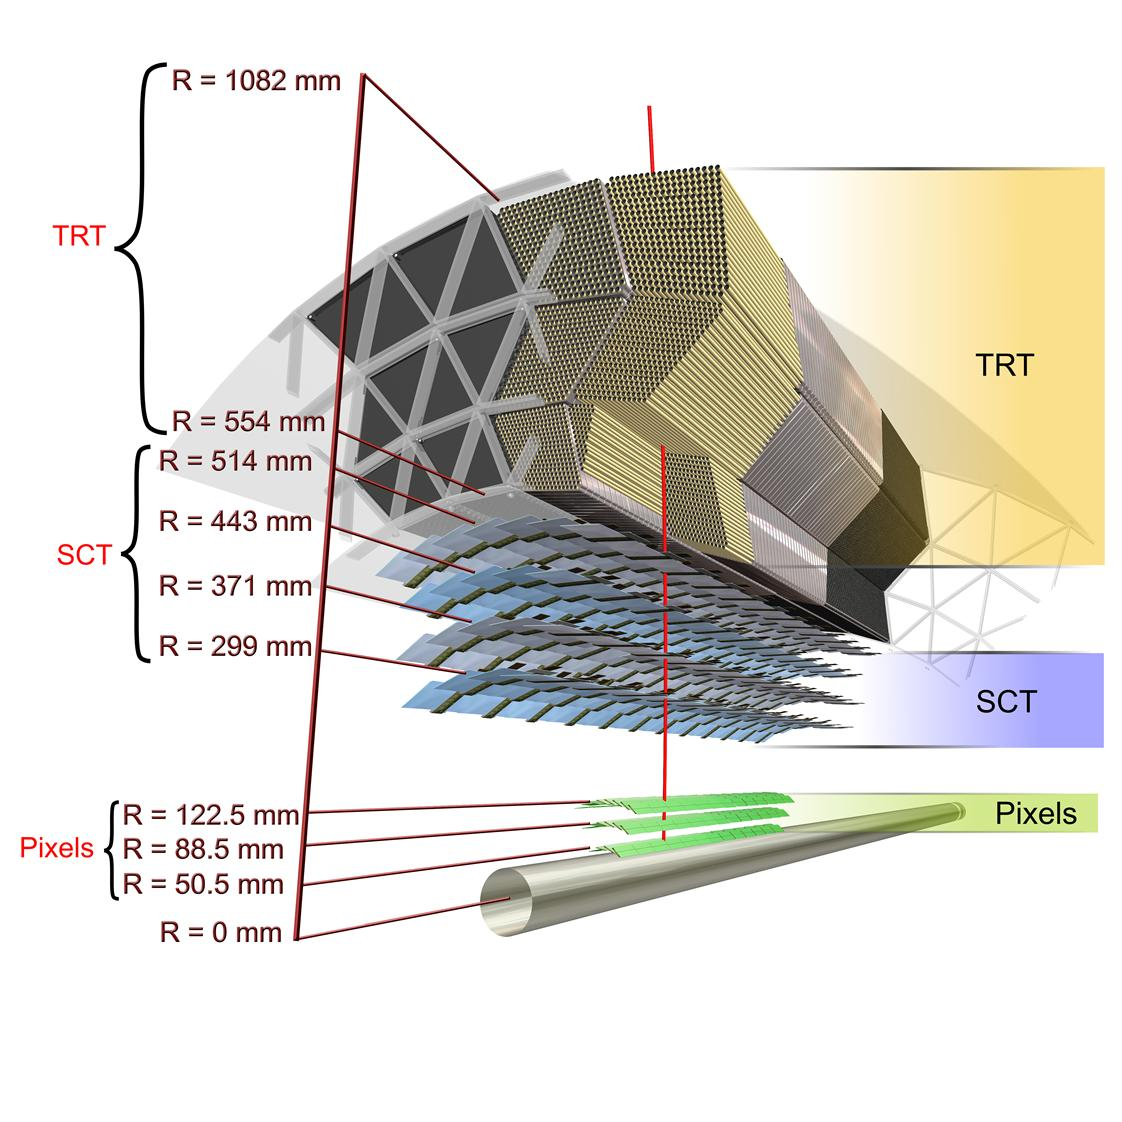
\includegraphics[width=0.75\textwidth]{figures/LHC/id_layout.jpg}
    \caption[]{ATLAS Inner Detector cut-away: Pixel Detector, Semiconductor Tracker, and Transition Radiation Tracker~\cite{Pequenao:1095926}.}
    \label{fig:id_layout}
\end{figure}

The first, the Pixel detector, consists of four layers of pixel detectors.
These pixel layers comprise a two-dimensional array of silicon pixels, providing high-precision measurements close to the interaction point.
The innermost layer is the Insertable B-Layer (IBL). The ``B'' in its name stands for ``Barrel,'' though the IBL is crucial in detecting short-lived particles, like hadrons with $b$ quarks. Due to its closeness to the interaction point, the IBL enhances the performance of the Pixel detector by improving the precisions of vertexing and track reconstruction.

The second subsystem, the SemiConductor Tracker (SCT), comprises four double layers of silicon strips. The SCT behaves similarly to the Pixel detector, except the measurement is one-dimensional. 
When a charged particle moves through a silicon layer, it bumps electrons to a higher energy level, creating ``holes'' in their place. This generates a current and signal the detector can read as a ``hit.''

The last subsystem is the Transition Radiation Tracker (TRT)~\cite{TheATLASTRTcollaboration_2008}, a straw tracker comprised of approximately 300,000 4 mm-diameter straw tubes. 
A straw tube is a long tube with a wire in the center filled with gas (Xenon). When a charged particle passes through, the gas becomes ionized, creating an electronic signal (a ``hit'').
The superconducting solenoid magnet bends the paths of charged particles based on their momentum, with the numerous hits in the TRT greatly enhancing momentum measurement accuracy.

\subsection{The Calorimeters}
The calorimeter system, enclosing the solenoid magnet and the inner detector, provides coverage up to \(|\eta| < 4.9\), although the coverage varies for each subdetector.
The calorimeters employs a fundamentally different detection method compared to the ID. While the ID is designed to track particles with minimal interaction, the calorimeters are designed to completely absorb the particles. This absorption prevents most particles from reaching further layers of detection. A significant advantage of calorimeters is their ability to detect neutral particles, with the exception of neutrinos. The calorimeter system comprises various subsystems, each responsible for covering a specific range of particles. Figure~\ref{fig:cal_layout} illustrates these subsystems.

\begin{figure}[ht]
    \centering
    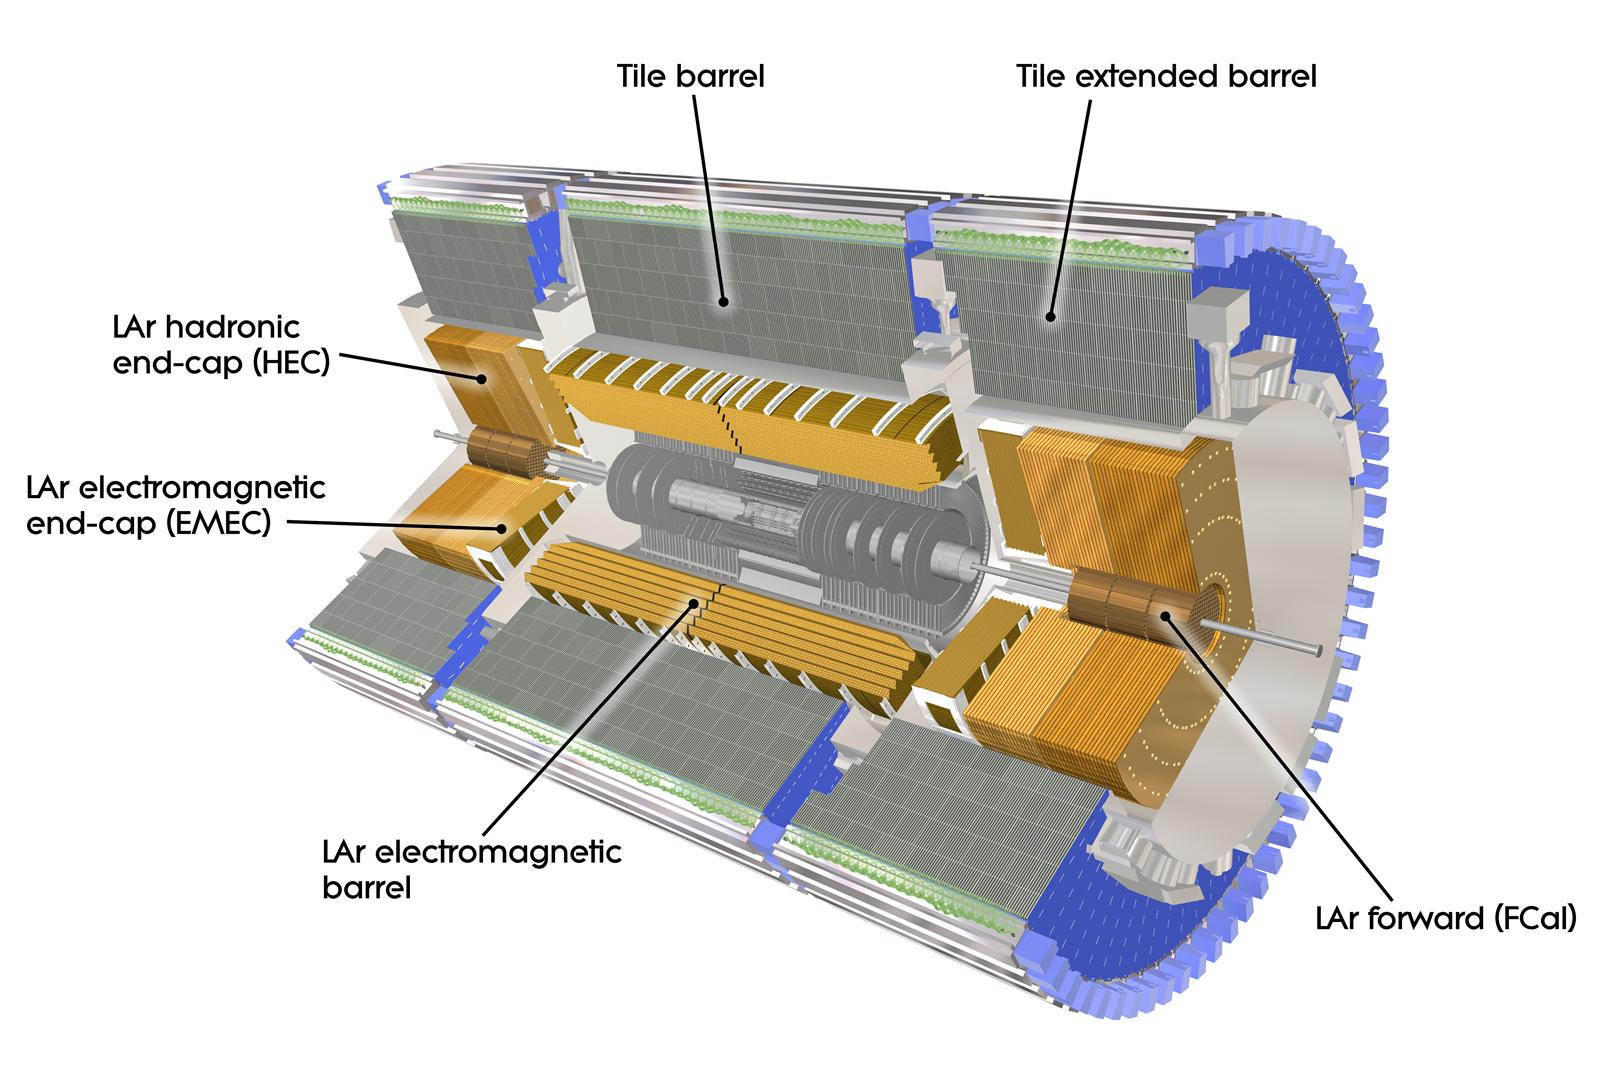
\includegraphics[width=0.75\textwidth]{figures/LHC/cal_layout.jpg}
    \caption[]{Cut-away view of the ATLAS calorimeter system~\cite{Pequenao:1095927}.}
    \label{fig:cal_layout}
\end{figure}

Calorimeters operate on a fundamental principle where particles enter a region filled with dense matter, leading to the creation of particle showers as they release their energy within the calorimeter. These devices are typically constructed from alternating layers of materials: a dense material that absorbs the particles, and a sampling material positioned between the absorber layers. The purpose of the sampling material is to detect the particle showers generated by the absorbers.
This detection is achieved through sensors connected to the sampling material. There are two prevalent types of sampling materials used in calorimeters: scintillating plastics and ionizable liquids. Scintillating plastics emit light when struck by particles and are read by photodiodes, while the ionizable liquids create ions that are detected by electrodes.

The innermost section of the calorimeter is occupied by the Electro-Magnetic Calorimeter (ECAL)~\cite{ATLAS:1996ab}. Noted for its unique accordion design, the ECAL ensures complete azimuthal coverage, eliminating gaps along the azimuthal direction. Despite this, a gap exists between the barrel and endcap sections of the ECAL along the $z$-direction, leading to a common practice of excluding particles within the pseudorapidity range of \(1.37 < |\eta| < 1.52\). The ECAL employs lead as the primary absorbing material, complemented by steel, and utilizes liquid argon as the sampling medium. Upon interaction with incoming particles, the liquid argon becomes ionized. These ionization events are then detected by electrodes shaped to match the accordion design of the calorimeter. The coverage of the ECAL extends to a pseudorapidity range of \(|\eta| < 3.2\).

The principal hadronic calorimeter, known as TileCAL~\cite{ATLAS:1996aa}, is designed to accommodate the penetrating nature of hadrons, which travel deeper into materials before stopping. TileCAL is considerably larger, utilizing steel as its absorbing material and scintillating plastic as the sampling material, ensuring effective energy measurement of hadrons. TileCAL is specifically engineered to cover a pseudorapidity range of \(|\eta| < 1.7\). In contrast, the endcaps of the calorimeter, which are constructed differently, employ copper as the absorbing material and liquid argon as the sampling medium. These endcaps extend the calorimeter's coverage to a range of \(1.5 < |\eta| < 3.2\), complementing TileCAL. Due to the endcaps being nested within TileCAL's structure, there is a significant degree of overlap between these components, ensuring that there are no gaps in the hadronic calorimeter's coverage.

The Forward Calorimeter (FCAL)~\cite{AArtamonov_2008} plays a crucial role in capturing particles that travel almost parallel to the beam line, essential for accurately measuring missing energy in experiments. Its design enables it to cover an extended pseudorapidity range of \(3.1 < |\eta| < 4.9\), significantly beyond the coverage of the central detectors. Although most physics analyses focus on events within a much narrower range, the ability of the FCAL to detect particles in this extended range is vital for ensuring that no energy goes unaccounted for, which is crucial for precision measurements. The FCAL comprises two distinct sections: an inner section with copper as the absorbing material and an outer section that utilizes tungsten. Liquid argon is employed as the sampling material across the entire FCAL, facilitating the detection and measurement of particle energies.


\subsection{The Muon Spectrometer}

The muon spectrometer (MS)~\cite{ATLAS:1997ad}, designed to detect muons within \(|\eta| < 2.7\), encircles the calorimeters and forms the detector's outermost layer. Its barrel region is defined in the range of \(|\eta| < 1.05\), with the endcap regions covering the remaining area.
The MS is supplemented by three large toroid magnets surrounding the calorimeters, bending the charged particles in the z direction with a strength of about \(2.5 \, \text{T}\cdot\text{m}\) in the barrel region and up to \(6 \, \text{T}\cdot\text{m}\) in the endcaps.
Only muons and neutrinos, due to their unique properties, can penetrate the calorimeters to reach the MS, which is specifically designed for precise measurements of muon momentum.
As seen in Figure~\ref{fig:muon_spec}, the trigger system of the muon system features the Resistive Plate Chamber (RPC) and Thin Gap Chamber (TGC). These trigger chambers offer bunch-crossing identification, well-defined transverse momentum (\pt) thresholds, and measurements of the muon's track coordinate~\cite{TheATLASCollaboration_2008}.
Combined with the corresponding measurements from the ID, one can determine all three components of a muon's momentum.

\begin{figure}[ht]
    \centering
    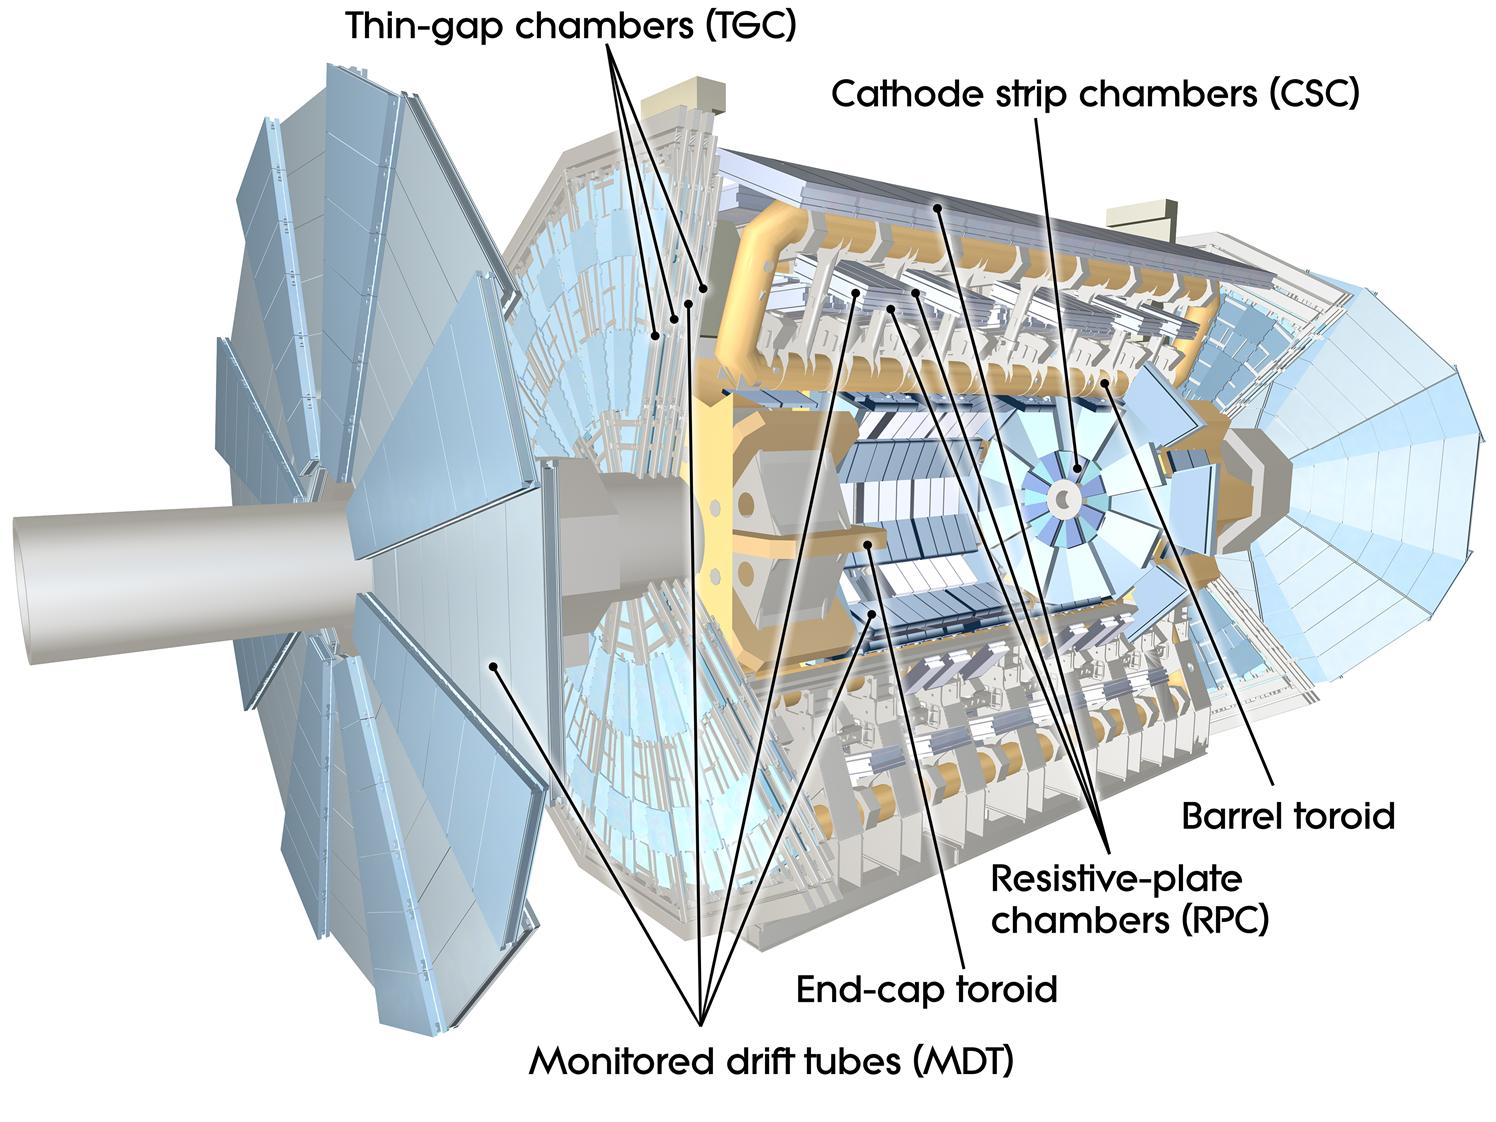
\includegraphics[width=0.75\textwidth]{figures/LHC/muon_spec.jpg}
    \caption[]{Cut-away view of the Muon Spectrometer system~\cite{Pequenao:1095929}.}
    \label{fig:muon_spec}
\end{figure}

%Pequenao:1095929


%TDAQ
\clearpage
\section{The Trigger and Data Acquisition}
\label{The_Trigger_and_Data_Acquisition}
The Trigger and Data Acquisition (TDAQ) system of ATLAS decides which events to record and store. As mentioned in Section~\ref{the_lhc}, the 25 ns spacing between proton bunches results in an event rate of 1 GHz, making real-time storage unfeasible.
Since the vast majority of the events aren't interesting for physics analysis here at ATLAS, TDAQ's goal is to reduce the collection rate to 1.5 kHz.
The trigger system is comprised of two triggers: the hardware-based Level 1 Trigger (L1)~\cite{ATLAS:1998ad} and the software-based High Level Trigger (HLT)~\cite{ATLAS:2003aa}.
Figure~\ref{fig:tdaq_layout} illustrates how the system works.

\begin{figure}[ht]
    \centering
    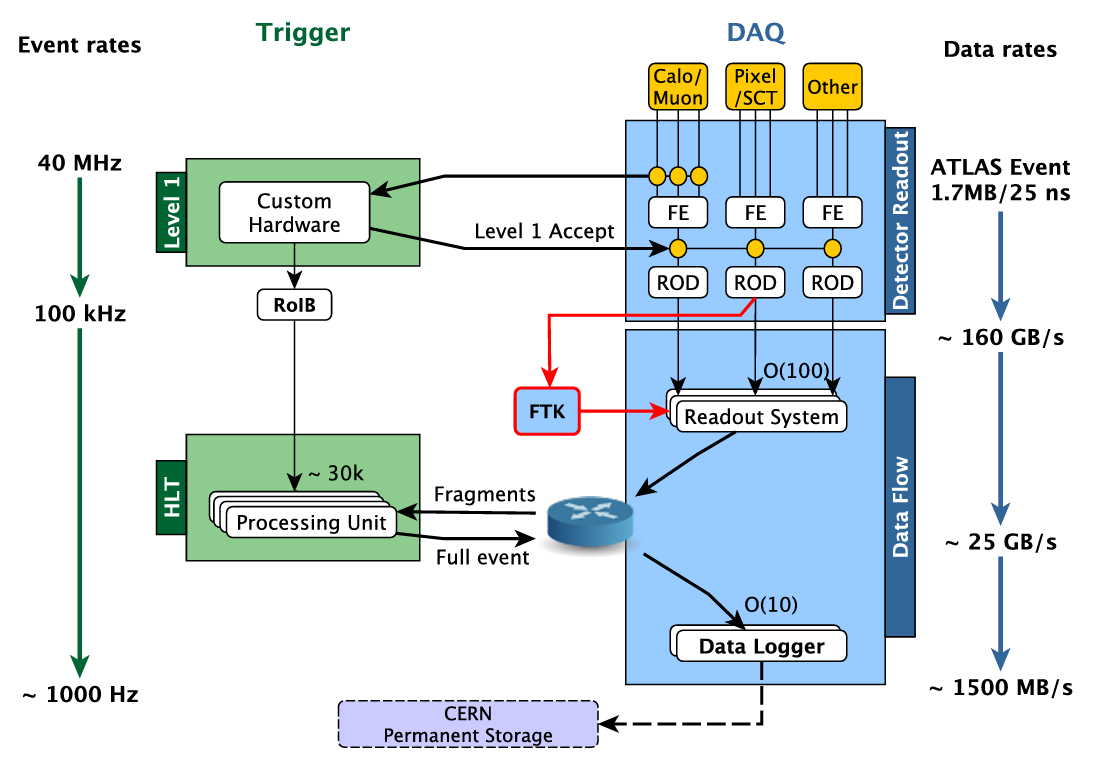
\includegraphics[width=0.85\textwidth]{figures/LHC/tdaq_1.png}
    \caption[]{ATLAS TDAQ Architecture~\cite{Abbott_2016}.}
    \label{fig:tdaq_layout}
\end{figure}

The L1 trigger, directly connected to the muon spectrometer and the calorimeters, identifies physics events with interesting objects such as high-momentum muons, significant missing energy, high-energy electrons/photons, or high-energy hadrons.
The dedicated hardware for the L1 trigger is situated within the same cavern as the ATLAS detector.
Events passing the L1 trigger are transferred from the detectors' Front End (FE) to the Read Out Drivers (ROD) at a reduced the event rate of 100 kHz.

The HLT includes the Level 2 Trigger (L2) and the Event Filter (EF). L1 identifies a region of interest (ROI) of the detector, and the complete event data within this ROI is forwarded to L2. 
``Tracking'' in the ROI is done by L2 to reconstruct the trajectory (or track) of electrically charged particles in the ID.
The tracks and calorimeter information are combined to refine the object selection with higher resolution than what was used in L1, such as tighter requirements on electrons, muons, and missing energy.
Events that pass L2 requirements are sent to the EF, which uses data from the entire detector to decide whether to keep the event.



%%%FTK
\section{Fast Tracker}

The Fast TracKer (FTK) system was foreseen as a significant upgrade for the TDAQ system of ATLAS by providing hardware-based tracking information directly to the HLT.
As discussed in Section 3.3, although the L1 trigger and HLT perform exceptionally in selecting physics events and reducing the event rate, this implementation does have its limitations.
Currently, the HLT receives the "hits" information recorded by the ID, essentially points in space, and conducts tracking calculations within the ROIs determined by the L1 trigger.
Tracking calculations in the HLT software are demanding and slow, leading to restrictions on the size and number of ROIs. 
The ROI approach also resulted in notable inefficiencies in jet finding, due to discrepancies between the online and offline strategies~\cite{TAMSETT2013253}~\cite{Aad2016}.
A solution is to use specialized hardware for this task, which is the primary goal of the FTK system. FTK will be positioned between the L1 trigger and HLT, offering tracking information for all events that pass the L1 trigger across the entire detector and supplying this data to the HLT.

The FTK system consists of various types of boards and components, with details provided in Figure~\ref{fig:ftk_overview} and Table~\ref{table:ftk_overview}. The Input Mezzanines (IM) receive data directly from the Level 1 trigger (the RODs). There are a total of 12 layers from the Inner Detector: four double SCT layers, three Pixel layers, and one IBL.
Clustering is applied to the hits from these layers to reduce data flow. The clustered data is then sent to the Data Formatter (DF) system.
The DF system divides the data, sending eight layers (five from the SCT and three from the Pixel) to the main Processing Units (PU) and the remaining four layers (three SCT and one IBL) to the Second Stage Boards (SSB).

\begin{figure}[ht]
  \centering
  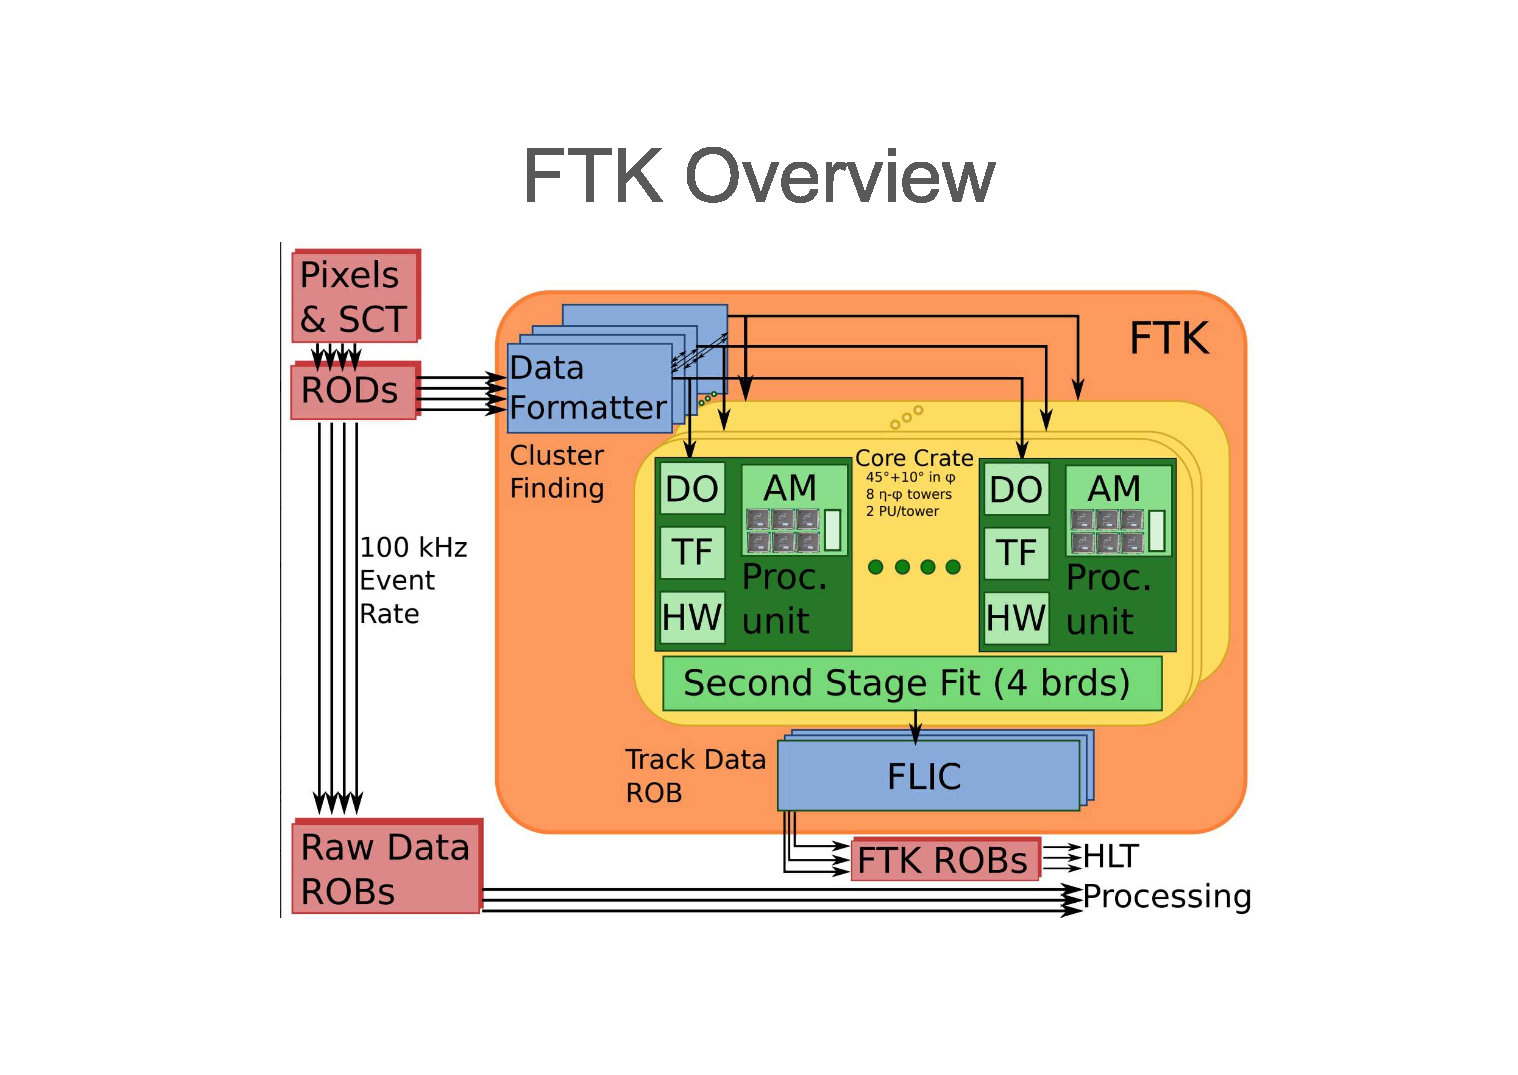
\includegraphics[width=0.95\textwidth]{figures/ftk/ftk_overview.pdf}
  \caption{Overview of the FTK system.}
  \label{fig:ftk_overview}
\end{figure}

\begin{table}[ht]
\centering
\resizebox{0.95\textwidth}{!}{%
\begin{tabular}{llllr}
\hline
\textbf{Module} & \textbf{Function} & \textbf{Type} & \textbf{Number} \\
\hline
\hline
IM & Input Mezzanine & Cluster Pixel and SCT hits, format module data & Mezzanine & 128 \\\hline
DF & Data Formatter & Transport and duplicate module hit data to \(\eta\)-\(\phi\) towers & ATCA & 32 \\\hline
AUX & Auxiliary Card & Transport coarse-resolution 8-layer hit data to AMB & VME & 128 \\\hline
AMB & AM Board & Transport hit data to AM & VME & 128 \\
AM & Associative Memory & Match hits to patterns & ASIC & 8192 \\
AUX & Auxiliary Card & Evaluate track candidates in matched patterns & VME & 128 \\\hline
SSB & Second Stage Board & Add remaining hits to 8-layer tracks, fit, remove overlaps & VME & 32 \\\hline
FLIC & HLT Interface Board & Interface to ATLAS readout & ATCA & 2 \\
\hline
\end{tabular}%
}
\caption{Overview of the FTK system in the order in which the data are processed. 
The AUX appears in the table twice because of its dual functions \cite{Aad_2021}.}
\label{table:ftk_overview}
\end{table}

The main Processing Units are made up of two boards: the Associated Memory Board (AMB) and the Auxiliary Board (AUX), with the AUX serving as a rear transmission module. The AMB is essential to the FTK system. To construct tracks rapidly, billions of precomputed tracks are stored in a large memory bank. These track patterns are then matched to the incoming hit coordinates using massive parallel processing. Each AMB can match eight million patterns in parallel to the incoming hit data.

The Auxiliary Board (AUX) communicates with its corresponding Associated Memory Board (AMB) via the VME backplane, performing a range of functions. Its principal duty involves eight-layer track fitting. The procedure is as follows:
\begin{itemize}
    \item Input data from the DF is forwarded to the AMB.
    \item The AMB, after matching patterns, returns them to the AUX.
    \item Utilizing these patterns, the AUX conducts a fit to assess their quality, allowing tracks to be missing a hit on one layer -- these are termed \textit{majority tracks} -- to boost efficiency.
    \item Moreover, the AUX undertakes the removal of duplicates among the eight-layer track candidates.
    \item Valid eight-layer tracks are then forwarded to the Second Stage Boards (SSB).
\end{itemize}

The Second Stage Board (SSB) system includes 32 boards, each responsible for managing tracks from four PUs. The SSB integrates these eight-layer tracks with hit data for the four additional layers from the corresponding DF, to assemble 12-layer tracks. This process involves:
\begin{itemize}
    \item Extrapolating the eight-layer track into the missing layers.
    \item Using hits near the extrapolated coordinates to fit full 12-layer tracks.
\end{itemize}
Like in the first stage, it is possible for tracks to be missing a hit in one of the new layers. After fitting, tracks undergo a global duplicate check before being forwarded to the FTK Level2 Interface Crate (FLIC). SSBs are paired to cover the entire detector range, with pairs linked in a ring to manage overlap.

The FTK Level2 Interface Crate (FLIC) is the last element in the FTK system, serving two primary purposes:
\begin{itemize}
    \item It merges the 12-layer track data from the 32 SSBs.
    \item It formats the consolidated data so that it can be interpreted by the Read Out System (ROS).
\end{itemize}

\subsection{Second Stage Board}

The Second Stage Boards (SSBs), designed and manufactured at the University of Illinois, perform three critical functions (see Figure~\ref{fig:ssb_board}):
\begin{itemize}
    \item Extrapolating incoming eight-layer tracks to include the missing layers,
    \item Fitting these extrapolations to form 12-layer tracks,
    \item Removing any duplicates found across the detector.
\end{itemize}
The hardware of the SSBs includes five Field-Programmable Gate Arrays (FPGAs) that require firmware. Four of these FPGAs, designated as the EXTF FPGAs, are dedicated to the tasks of extrapolation and track fitting. The fifth FPGA, known as the Hit Warrior (HW) FPGA, is tasked with duplicate removal. Furthermore, the SSBs are equipped with a substantial amount of Reduced Latency Dynamic Random-Access Memory (RLDRAM) for storing the constants necessary for extrapolation and track fitting calculations.
The layout and the dataflow through the SSB are shown in Figure~\ref{fig:ssb_diagram}.

\begin{figure}[ht]
  \centering
  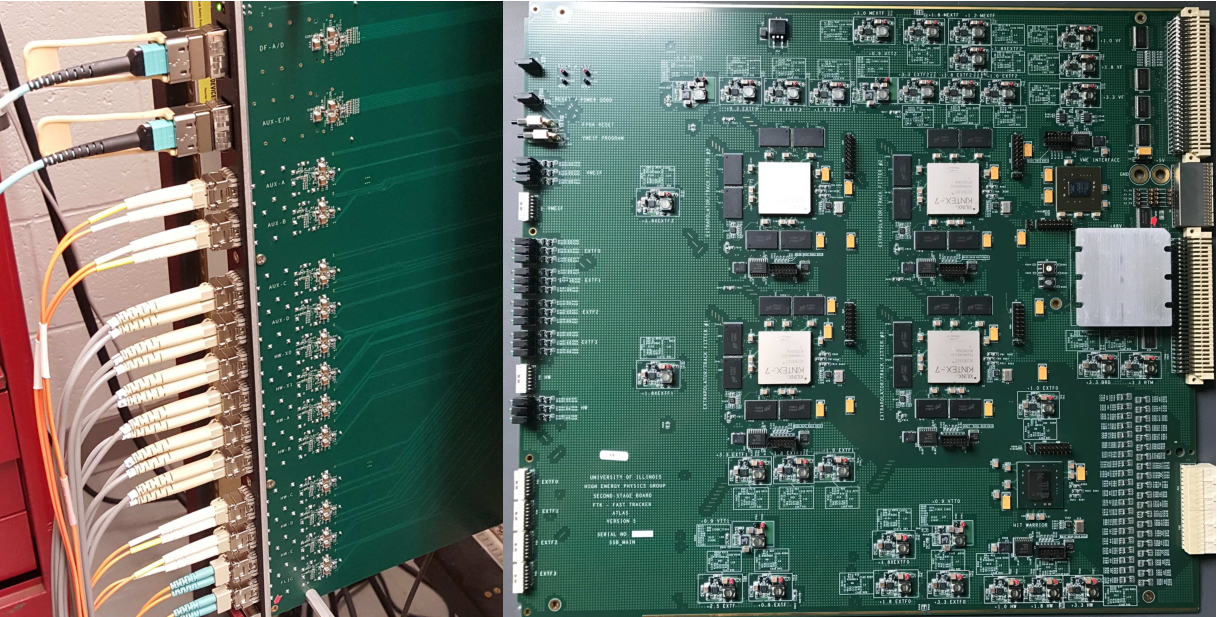
\includegraphics[width=0.75\textwidth]{figures/ftk/ssb_board.pdf}
  \caption{The physical Second Stage Boards~\cite{Aad_2021}.}
  \label{fig:ssb_board}
\end{figure}

\begin{figure}[ht]
  \centering
  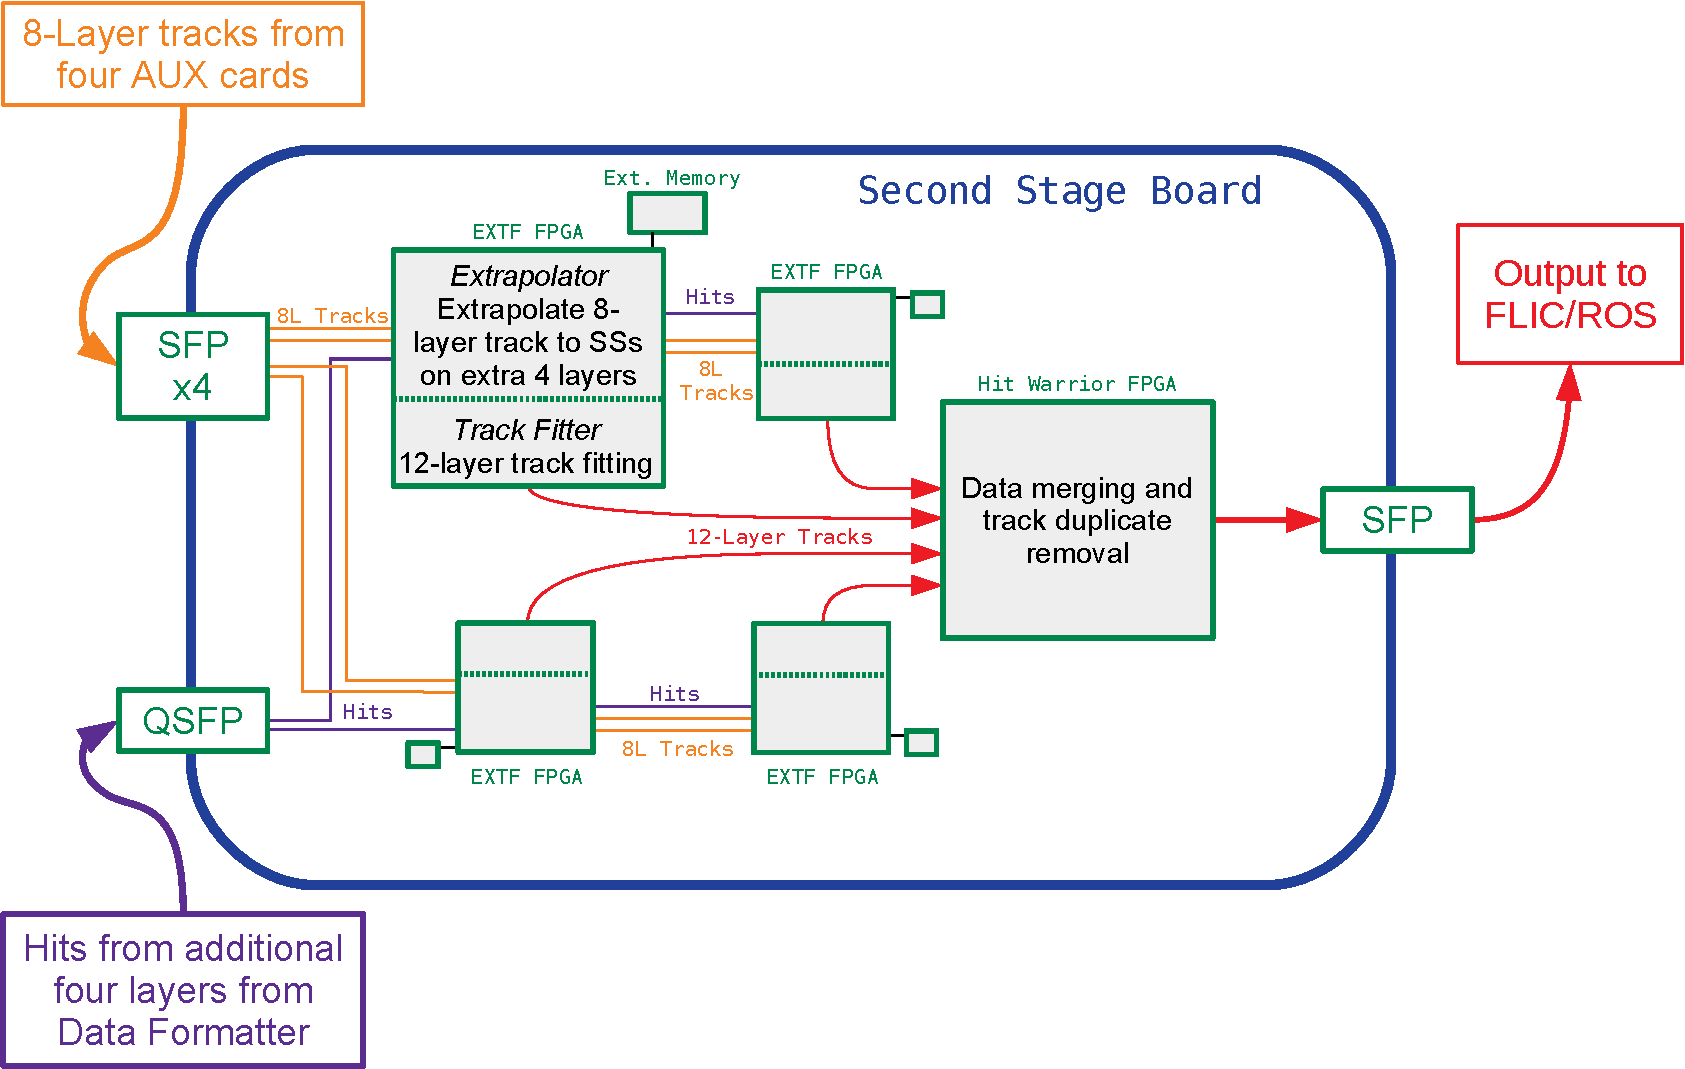
\includegraphics[width=0.75\textwidth]{figures/ftk/ssb_diagram.pdf}
  \caption{Diagram of the dataflow through the Second Stage Board~\cite{Aad_2021}.}
  \label{fig:ssb_diagram}
\end{figure}

The core functionality of the EXTF FPGA is allocated to the Extrapolator (EXP), which oversees the extrapolation process, and the Track Fitter (TF), focused on the fitting of the resulting 12-layer tracks. For a thorough exploration of these firmware aspects, see Markus Atkinson's PhD thesis \cite{Atkinson2019}.

\subsection{Hit Warrior FPGA}
The Hit Warrior FPGA on the SSB serves two key roles. Its main job is to eliminate duplicate tracks. Its second role involves merging data. Each SSB houses four EXTF FPGAs, and the Hit Warrior FPGA collects all their output. This output is then scanned for any duplicates, combined into a single large output packet, and forwarded to the FLIC.
The top-level diagram of the Hit Warrior firmware design is depicted in Figure~\ref{fig:hw_top_diagram}. In the diagram, the Sync Engine module synchronizes the four incoming EXTF streams. The Hit Warrior module is the logic component that performs the comparison and duplicate removal tasks. Additionally, Spy Buffers are utilized for monitoring purposes. More details on the Hit Warrior module follow.

\begin{figure}[ht]
  \centering
  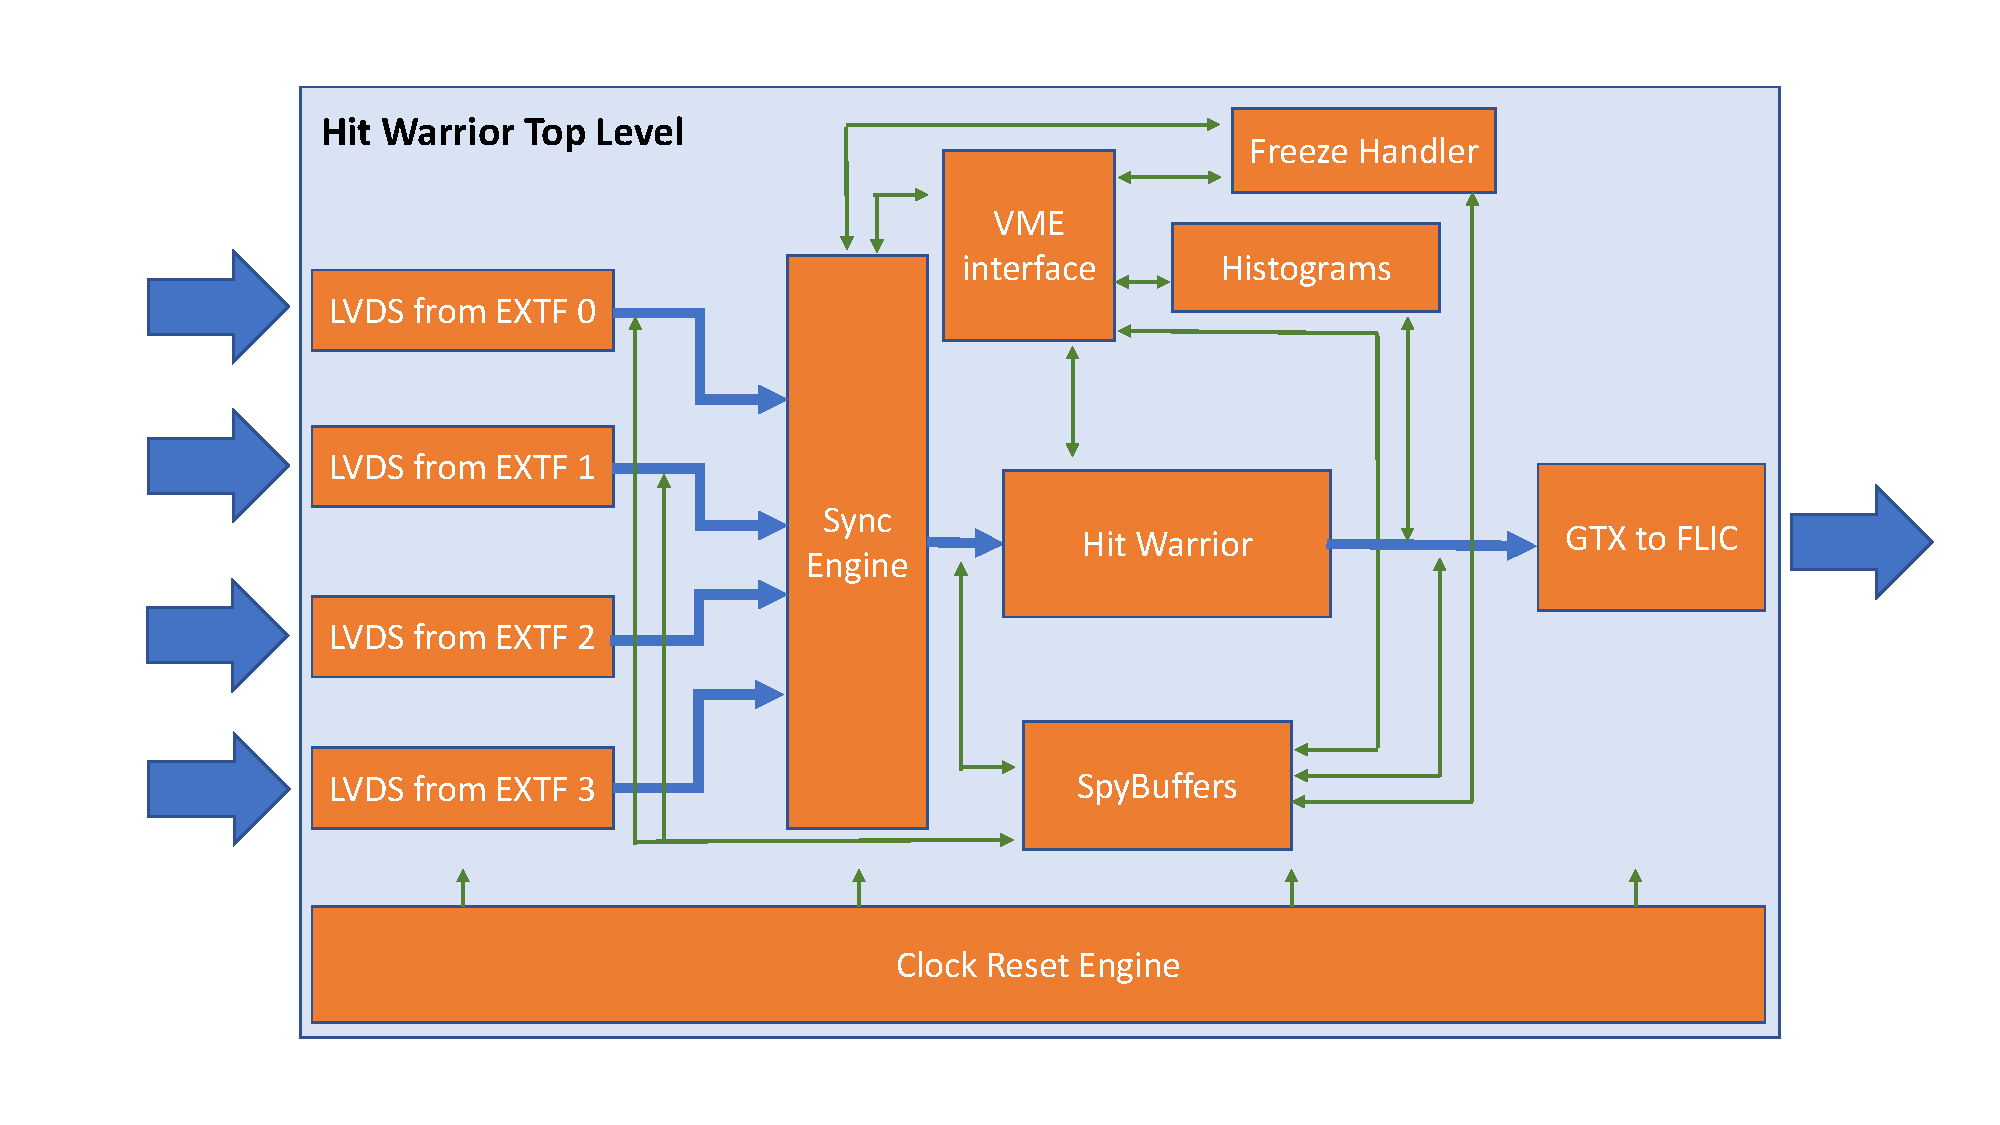
\includegraphics[width=0.75\textwidth]{figures/ftk/hw_top_diagram.pdf}
  \caption{Diagram of the Hit Warrior firmware~\cite{Aad_2021}.}
  \label{fig:hw_top_diagram}
\end{figure}

The Track Parser functions as the first component of the Hit Warrior module, where it examines the data to identify the start of track packets. These packets always start with the keyword ``BDA'' and consist of 28 words. Each track is distributed throughout the FPGA to enable parallel processing of track comparisons. Tracks are processed sequentially, one after another, which makes it practical to use a track counter. The specific processing path for each track depends on this counter. However, the overarching strategy ensures that each new track is compared with all previously received tracks simultaneously. By the time the final track is processed, all necessary track comparisons have been completed.

The first and simplest component to understand in this context is the RAW FIFO (First In, First Out). This acts as an internal storage or buffer for all the tracks corresponding to the current event, storing them in the exact order they were received.
The layout is illustrated in Figure \ref{fig:hw_fifo}.

\begin{figure}[ht]
  \centering
  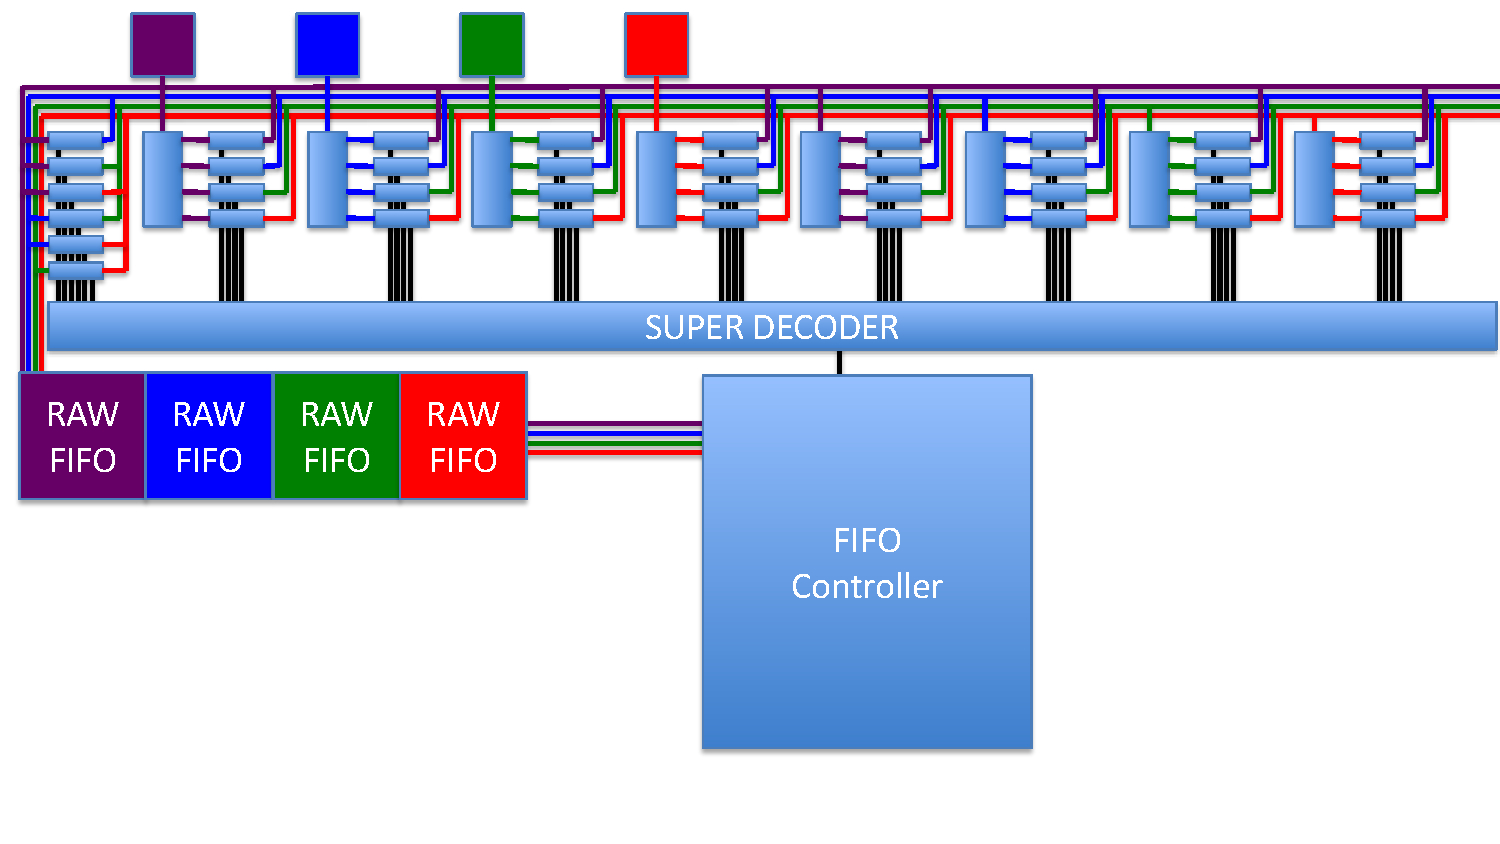
\includegraphics[width=0.75\textwidth]{figures/ftk/hw_fifo.pdf}
  \caption{Hit Warrior FIFO Diagram}
  \label{fig:hw_fifo}
\end{figure}

Tracks are also sent to units called Comparators. The total number of Comparators is limited by available resources, which in turn sets a maximum on the number of tracks that can be effectively compared for an event. Each Comparator is equipped with a small piece of RAM (Random Access Memory) capable of holding a single track packet. Furthermore, each Comparator is directly connected to the stream of incoming tracks, allowing it to receive and compare new track data as it arrives.

%%%Comparators
The comparator conducts comparisons between two tracks on a word-to-word basis to identify matches. Each track packet contains 28 words, comprising 12 for the Track Header and 16 for the hit list. These 16 words are distributed across 12 layers. A match requires at least eight layers to be identical, a criterion determined through simulation to ensure maximum efficiency. For 2D pixel layers, both coordinates must match.

When matches are detected, a selection criterion decides the optimal track. Tracks with the same number of layers are evaluated on their \(\chi^2\) values to select the best one. If the layer count varies, the track with the greater number of layers is chosen. The selection scheme is outlined in the Table~\ref{table:track_selection_scheme}.

\begin{table}[ht]
\centering
\resizebox{0.6\textwidth}{!}{%
\begin{tabular}{ccc}
\hline
\textbf{Track 1} & \textbf{Track 2} & \textbf{Decision} \\
\hline
Nominal & Nominal & Select Track with lowest \(\chi^2\) \\
Nominal & Majority & Select Nominal Track \\
Majority & Majority & Select Track with lowest \(\chi^2\) \\
\hline
\end{tabular}%
}
\caption{Selection scheme for matching tracks.}
\label{table:track_selection_scheme}
\end{table}

After each track is compared, the outcome is forwarded to the Decoder, which logs the results of all track comparisons. Each comparator can issue one of four possible outcomes, encoded as two bits: \textit{idle}, \textit{no match}, \textit{delete RAM}, and \textit{delete Stream}. The Decoder synthesizes these outcomes with the current track count and the comparator's index to generate a "copy vector." This vector is essential for managing the write process to the CUT FIFO.

Once every track for the event has been examined and the copy vector is complete, the RAW FIFO's content is moved. This FIFO contains a copy of every track. This data is then transferred to a second FIFO, named the CUT FIFO, guided by the copy vector to ensure only the valid tracks are preserved. This arrangement allows for the removal of gaps in the data by excluding the tracks as dictated by the copy vector.

\begin{table}[ht]
\centering
\begin{tabular}{ll}
\hline
\textbf{Comparator Output} & \textbf{Meaning} \\
\hline
Idle & No operation \\
No Match & No duplicate found \\
Delete RAM & Remove track from RAM \\
Delete Stream & Remove track from incoming stream \\
\hline
\end{tabular}
\caption{Comparator Results and Their Meanings}
\label{table:comparator_results}
\end{table}

The CUT FIFO then serves as the final repository for the processed tracks, ensuring that only the relevant tracks are stored for further processing.
The decoder, using comparator flags, the index number of each comparator, and the track counter, identifies tracks for deletion. For instance, comparator M can only eliminate track M stored in its RAM or the track currently indexed by the track counter. Each processed track is compared in parallel to all prior ones. In each comparison round, any previous track might be marked for deletion by the incoming track. After each round, the decoder updates the copy vector to record any tracks flagged for removal. When the last track of the event has been compared, the final version of the copy vector is used to regulate the transfer of data from the RAW FIFO to the CUT FIFO, ensuring only the required tracks are retained.

It became apparent later in development that the prototype Hit Warrior firmware couldn’t keep up with the required processing speed. To address this, the system was adapted to process multiple streams in parallel. The Parallel Hit Warrior operates much like the original but at quadruple the speed by handling four streams simultaneously. This choice is aligned with the four EXTF FPGAs on each SSB. Therefore four tracks are inputted into four separate comparators. These comparators have been adapted to match a track in RAM against four incoming stream tracks at the same time. Additionally, a new component, the Cross Comparator, was introduced to compare all six pairings among the four stream tracks.
The layout of the Parallel Hit Warrior is shown in Figure \ref{fig:hw_layout}, and the details of the comparator are revealed in Figure \ref{fig:hw_details}.

\begin{figure}[ht]
  \centering
  \begin{subfigure}[b]{0.5\textwidth}
    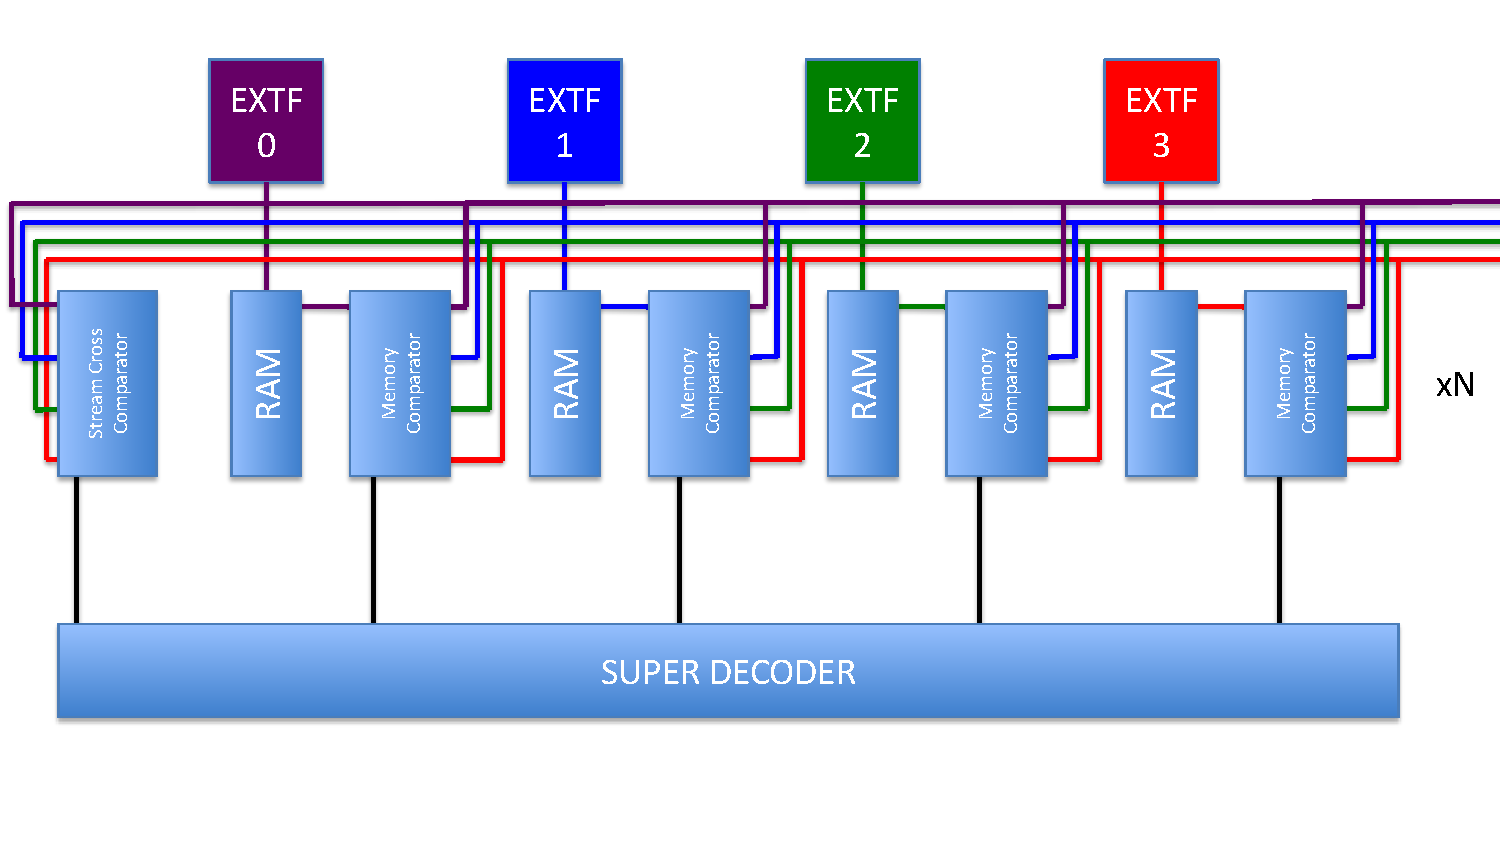
\includegraphics[width=\textwidth]{figures/ftk/hw_layout.pdf}
    \caption{Hit Warrior Layout}
    \label{fig:hw_layout}
  \end{subfigure}%
  \hfill
  \begin{subfigure}[b]{0.5\textwidth}
    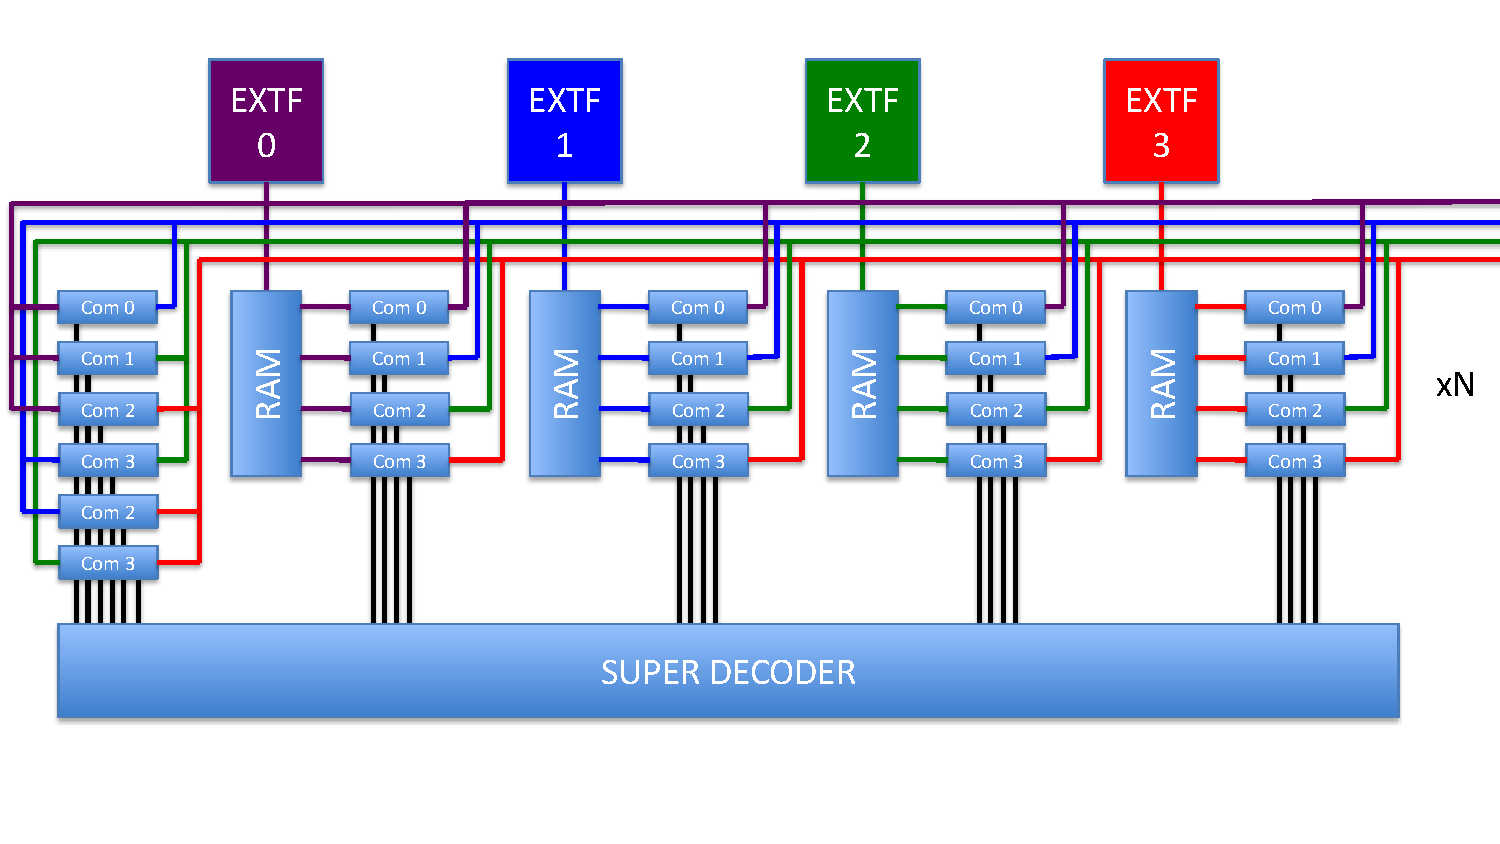
\includegraphics[width=\textwidth]{figures/ftk/hw_details.pdf}
    \caption{Hit Warrior Details}
    \label{fig:hw_details}
  \end{subfigure}
  \caption{Hit Warrior System Components}
  \label{fig:hit_warrior}
\end{figure}

%Spybuffer
The firmware design for the HitWarrior FPGA utilizes circular buffers, known as Spy Buffers, to capture data as it moves through the system, alongside the capability to read out monitoring registers. It also allows for the freezing of monitoring data in the event of errors to aid in debugging. Furthermore, these buffers store synchronized monitoring information and compile histograms of monitoring data. While this firmware design is broadly applied across various components of the FTK system, including the design of synchronization blocks, the SSB version is tailored for the HitWarrior FPGA to meet specific design needs and to accommodate the architecture of the FPGA chip.
As shown in Figure~\ref{fig:hw_top_diagram}, the Spy Buffers monitor the four parallel streams from the EXTF FPGAs, and the output of the Hit Warrior module before sending it to the FLIC.

%my job

My role in the development of the SSB involved updating the firmware for the Hit Warrior FPGA, focusing on parallelizing the prototype Hit Warrior firmware and implementing the Spy Buffers. 
I was deeply involved, often as the sole representative for the SSB, in its commissioning and integration into the ATLAS trigger system. This required extensive hours in the ATLAS control rooms and the underground facilities where the FTK system is installed.




























%\section{The LHC}
%\section{The ATLAS Detector}
%\subsection{The Inner Detector}
%\subsection{The Calorimeters}
%\subsection{The Muon Spectrometer}
%\section{The Trigger and Data Acquisition}
%\subsection{Fast Tracker}

\chapter{Experimental Methods}
%%% DataMCSamples %%%
\label{ch:exp_methods}
%%%This section contains information about the various data and Monte Carlo samples used in this analysis.

\section{Data Samples}
\label{sec:data_sample}

%%%
The semileptonic VBS analysis is based on proton-proton (\pp) collision data collected from 2015 to 2018, amounting to an integrated luminosity of \intLumi\,\ifb. The overall uncertainty for the integrated luminosity, measured at 1.7\%\cite{ATLAS-CONF-2019-021}, was determined using the LUCID-2 (LUminosity Cherenkov Integrating Detector)~\cite{Avoni:2633501} for primary luminosity measurements.
Table~\ref{tab:intLumi} summarizes the integrated luminosity used in this analysis.


\begin{table}[htb!p]
\begin{center}
\caption{Integrated luminosity data used in the semileptonic VBS analysis.}
\label{tab:intLumi}
\begin{tabular}{|l|c|}
\hline
Year & $\mathcal{L}$ [\ifb] \\
\hline\hline
2015 & 3.21 \\
\hline
2016 & 32.88 \\
\hline
2017 & 44.31 \\
\hline
2018 & 58.45 \\
\hline\hline
total & $139.0 \pm 2.4$ \\
\hline
\end{tabular}
\end{center}
\end{table}



\section{Monte Carlo Simulated Samples}
\label{sec:mc_sample}
%Lists of MC samples for both the SM background and EW signal processes signals are summarized in appendix \ref{app:samplelist}.

Monte Carlo (MC) simulations are integral to nearly all stages of the analysis workflow. These simulations are essential for background modeling, signal acceptance evaluation, event selection optimization, systematic uncertainty estimation, and statistical analysis.
The MC samples are generated with ATLAS-approved settings.
The EvtGen v1.2.0 program~\cite{Lange:2001uf} simulates bottom and charm hadron decays. 
To account for pileup, additional $pp$ collisions are simulated using \textsc{Pythia} 8.186\cite{Sjostrand:2008vc} and integrated into all MC events. 
The samples undergo a comprehensive simulation of the ATLAS detector\cite{SOFT-2010-01} using \textsc{GEANT4}\cite{Agostinelli:2002hh}.
All simulated events are processed using the same trigger and reconstruction algorithms as the collected data.
Appendix \ref{app:samplelist} summarizes the MC samples for SM background and EW signal processes.



\subsubsection{Background processes}
\label{sec:bg_mc_sample}
The $V$ ($W/Z$) + jets events are simulated with Sherpa 2.2.1~\cite{Gleisberg:2008ta} and normalzied to the NNLO cross sections. 
Up to 2 partons at NLO and 4 partons at LO are considered using Comix~\cite{Gleisberg:2008fv} and OpenLoops~\cite{Cascioli:2011va} for matrix element calculations, integrated with the Sherpa parton shower~\cite{Schumann:2007mg} using the ME+PS@NLO prescription~\cite{Hoeche:2012yf}. 
These simulations use the NNPDF3.0NNLO PDF set alongside specific tuning~\cite{Ball_2015}. 
%% $W$/$Z$ + jets samples are normalzied to the NNLO cross sections.

As alternative \Vjets MC samples for the analysis, QCD $V$+jets production was simulated using \MGNLO[2.2.2]~\cite{Alwall:2014hca} with LO-accurate matrix elements (ME) featuring up to four final-state partons. 
These ME calculations utilized the \NNPDF[3.0nlo] PDF set~\cite{Ball:2014uwa} for $H_\text{T}$-sliced and the \NNPDF[2.3lo] set~\cite{Ball:2012cx} for $N_\text{parton}$-sliced events. 
The events were then interfaced with \PYTHIA[8.186]~\cite{Sjostrand:2007gs} to simulate the parton shower, hadronization, and the underlying event dynamics.
The CKKW-L merging procedure~\cite{Lonnblad:2001iq,Lonnblad:2011xx} was applied to eliminate overlap between matrix element calculations and parton shower emissions.
The A14 tune of \PYTHIA[8]~\cite{ATL-PHYS-PUB-2014-021}, in conjunction with the \NNPDF[2.3lo] PDF set~\cite{Ball:2012cx}, was used. 
Decays of bottom and charm hadrons were handled by \EVTGEN[1.2.0]~\cite{Lange:2001uf}. 
Although not the nominal samples, these $V$+jets samples were normalized to NNLO predictions~\cite{Anastasiou:2003ds} and served to derive modeling uncertainties for the \Vjets background.

The \ttbar and single-top events are generated using Powheg-Box~\cite{Alioli:2010xd} and NNPDF3.0NLO PDF sets~\cite{Ball:2014uwa} for matrix element calculations, ensuring top quark spin correlations are preserved. 
Specifically, t-channel top quarks are decayed with MadSpin~\cite{Artoisenet:2012st}. 
\textsc{Pythia}8.230 simulates the parton shower, fragmentation, and underlying event dynamics using the A14 tune set~\cite{ATL-PHYS-PUB-2014-021}, with the top quark mass set at $172.5\gev$. 
The cross sections for \ttbar and single-top processes are calculated with NNLO precision in QCD, which includes the re-summation of next-to-next-to-leading logarithmic (NNLL) soft gluon terms~\cite{Czakon:2011xx,Kidonakis:2011wy,Kidonakis:2010tc,Kidonakis:2010ux}.
The \textsc{Hdamp} parameter, which regulates high-\pt\ radiation in \textsc{Powheg}, is set to $1.5m_{t}$ to ensure good data/MC agreements in the high-\pt\ region\cite{ATL-PHYS-PUB-2016-020}.

The $q\bar{q}$-induced diboson processes ($WW$, $WZ$, and $ZZ$) are simulated using \SHERPA[2.2.1] or 2.2.2~\cite{Bothmann:2019yzt}, as per the specific process. 
These simulations incorporate off-shell effects and, where relevant, Higgs boson contributions. 
The matrix elements are calculated with NLO QCD accuracy for up to one additional parton and LO accuracy for up to three additional partons.

Loop-induced $gg \to VV$ processes were simulated using LO-accurate matrix elements with up to one additional parton emission, covering both fully leptonic and semileptonic final states. These calculations were harmonized and combined with the \SHERPA parton shower via Catani--Seymour dipole factorisation~\cite{Gleisberg:2008fv,Schumann:2007mg}, following the MEPS@NLO prescription~\cite{Hoeche:2011fd,Hoeche:2012yf,Catani:2001cc,Hoeche:2009rj}.

QCD diboson production from $gg$ initial states is excluded from the final results due to its significantly smaller expected cross section compared to the baseline QCD $VV$ production; their impact has been evaluated and found to be negligible.


\subsubsection{Signal SM EW VV+jj processes}
\label{sec:mc_sample_ewvvjj}

The EW $VV+jj$ production is simulated with MadGraph5\_aMC@NLO v2.3.3~\cite{Alwall:2014hca} and \PYTHIA8~\cite{Sjostrand:2007gs} for fragmentation, using the \textsc{NNPDF30NLO} PDF set~\cite{Ball:2012cx}. 
The samples feature two on-shell $V$ bosons: one decaying leptonically ($Z \to \ell\ell$ where $\ell = e, \mu$; $Z \to \nu\nu$; $W \to \ell \nu$ with $\ell= e, \mu, \tau$), and the other hadronically. 
Both $W^{+}$ and $W^{-}$ decays are included, and for $WWjj$, all charge combinations ($W^{+}W^{+}$, $W^{+}W^{-}$, and $W^{-}W^{-}$) are considered. 
Table~\ref{tab:VBS_sig_samples} details the EW $VV+jj$ samples used in this analysis.
In these samples, we account for all purely-electroweak tree-level diagrams of order $\mathcal{O}(\alpha_{EW}^6)$ that contribute to the final states. This includes both VBS diagrams and non-VBS electroweak diagrams. Detailed examples of these diagrams have been previously discussed and are showcased in Figures~\ref{fig:feynmanVBS} and \ref{fig:feynmanEWKnonVBS}, as found in Section~\ref{section:Vector_Boson_Scattering}.


For EW $WW+jj$ production, the non-VBS electroweak $t\bar{t}$ diagrams, as depicted in Fig.~\ref{fig:feynmanEWKnonVBS}(e) and (f), could significantly contribute. This potential issue is effectively mitigated through the use of a $b$-veto. Despite this mitigation, the contribution from the non-VBS $tZb$ process, illustrated in Fig.~\ref{fig:feynmantZb}, remains considerable. To address this, a cut was implemented near the reconstructed top mass, effectively reducing its impact, as detailed in Table~\ref{tab:1lep_resolved}.

Diagrams that feature both electroweak and QCD vertices, with an order of $\mathcal{O}(\alpha_{EW}^{4} \alpha_s^{2})$, are not included in these signal samples and are not part of the signal definition.
Examples of such diagrams are depicted in Fig.~\ref{fig:feynmanQCD}. These processes, unaffected by aQGCs, are considered part of the background, including $t\bar{t}$, single-top, and diboson events.

%%%fixed eff
\begin{table}[!htbp]
\begin{center}
\small
\caption{List of VBS samples used in the analysis.}
\begin{tabularx}{\textwidth}{|c|c|X|X|X|c|c|c|}
\hline
Process & DSID & Events - mc16a & Events - mc16d & Events - mc16e & Filter efficiency & cross-section~(pb) \\
\hline

$\Wlv\Wqq jj, b-veto$    & 364848   &   1958000 &  2296000 & 3320000 & 0.17465  &  1.9994  \\
$\Wlv\Wqq jj, b-filter$  & 364849   &   1996000 &  2400000 & 3388000 & 0.83126  &  1.9777  \\
$\Wlv\Zqq jj$            & 364850   &   1994000 &  2394000 & 3392000 & 1.0  &  0.2571  \\
$\Zvv\Wqq jj$            & 364851   &   1986000 &  2394000 & 3356000 & 1.0  &  0.15532  \\
$\Zll\Wqq jj$            & 364852   &   1996000 &  2374000 & 3390000 & 1.0  &  0.045609  \\
$\Zvv\Zqq jj$            & 364853   &   1998000 &  2396000 & 3390000 & 1.0  &  0.032238  \\
$\Zll\Zqq jj$            & 364854   &   1990000 &  2388000 & 3396000 & 1.0  &  0.0096553  \\

\hline
\end{tabularx}
\label{tab:VBS_sig_samples}
\end{center}
\end{table}

%% feynman diagram, tZb
\begin{figure}[tbp]
\begin{center}
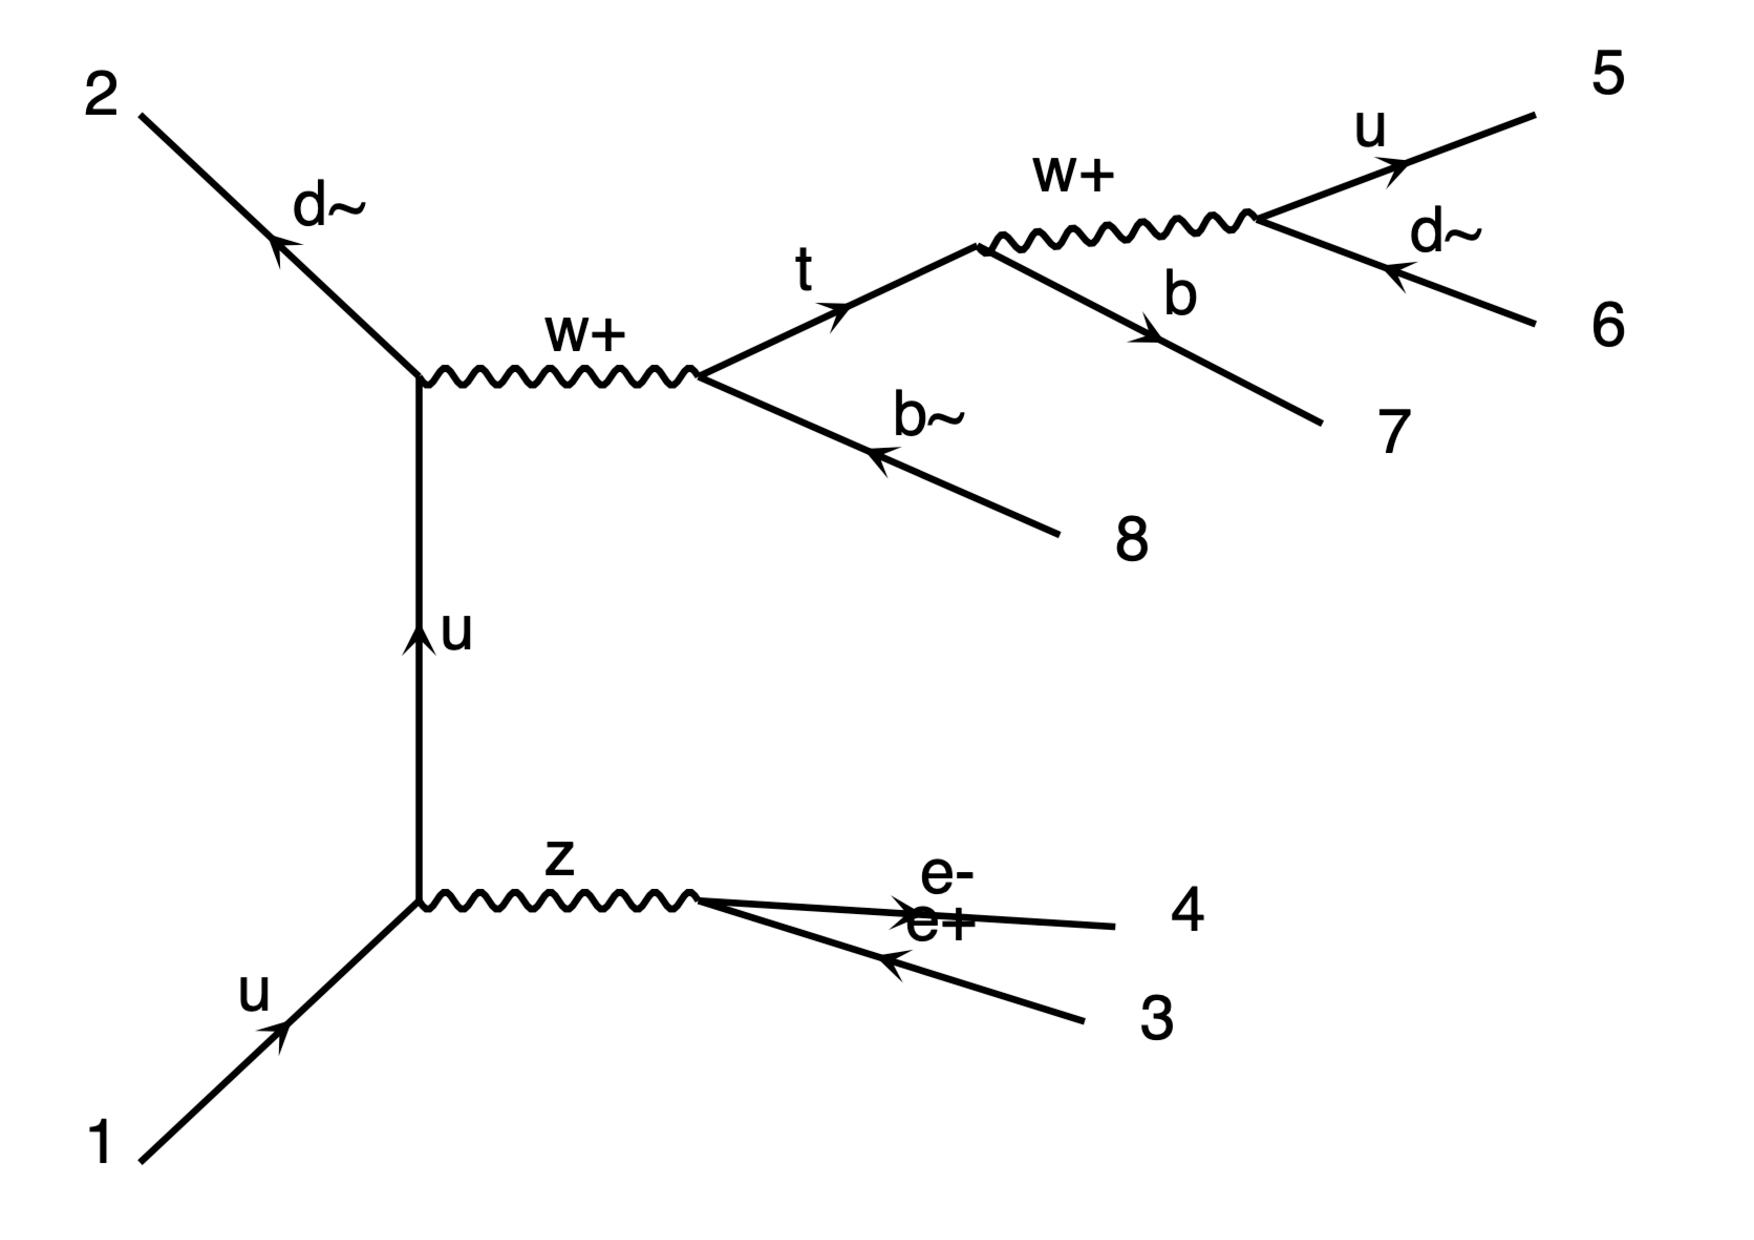
\includegraphics[width=0.35\textwidth]{figures/samples/feynEWKnonVBStZb.pdf}
\caption{
The example of the tZb diagram, which included in non-VBS $\mathcal{O}(\alpha_{EW}^6)$ diagrams. 
}
\label{fig:feynmantZb}
\end{center}
\end{figure}
%% feynman diagrams, QCD
%
\begin{figure}[tbp]
\begin{center}
\subfloat[]{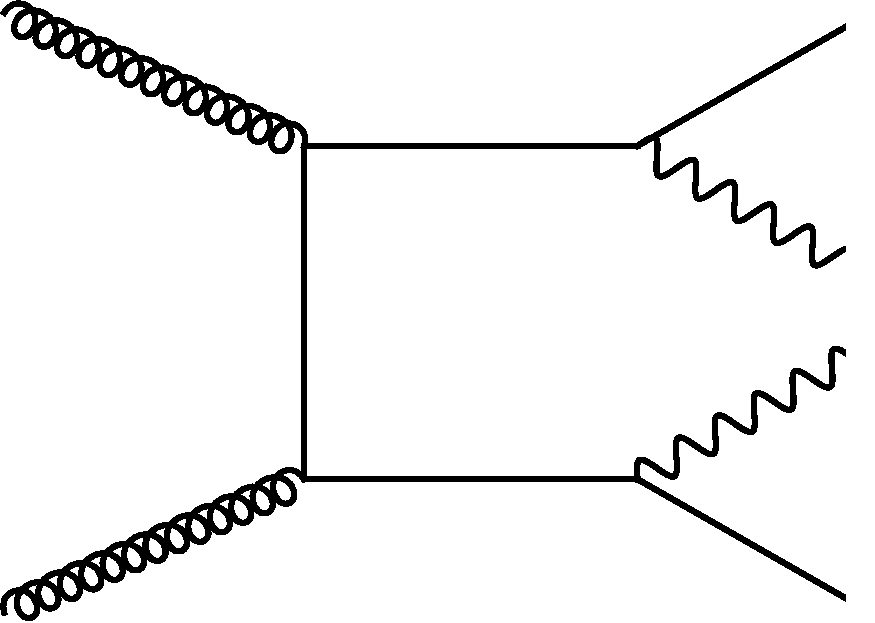
\includegraphics[width=0.3\textwidth]{figures/samples/feynQCD3.pdf}}
\subfloat[]{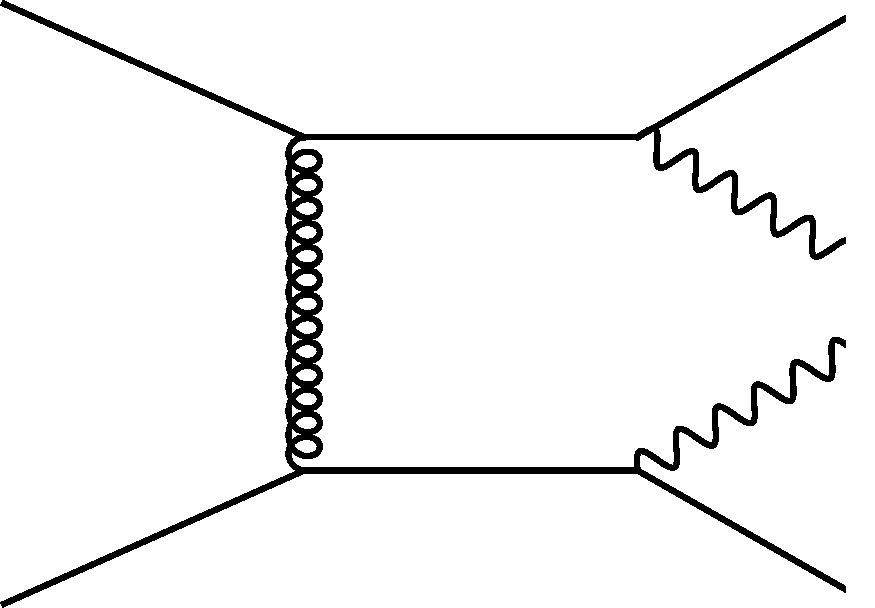
\includegraphics[width=0.3\textwidth]{figures/samples/feynQCD4.pdf}}
\subfloat[]{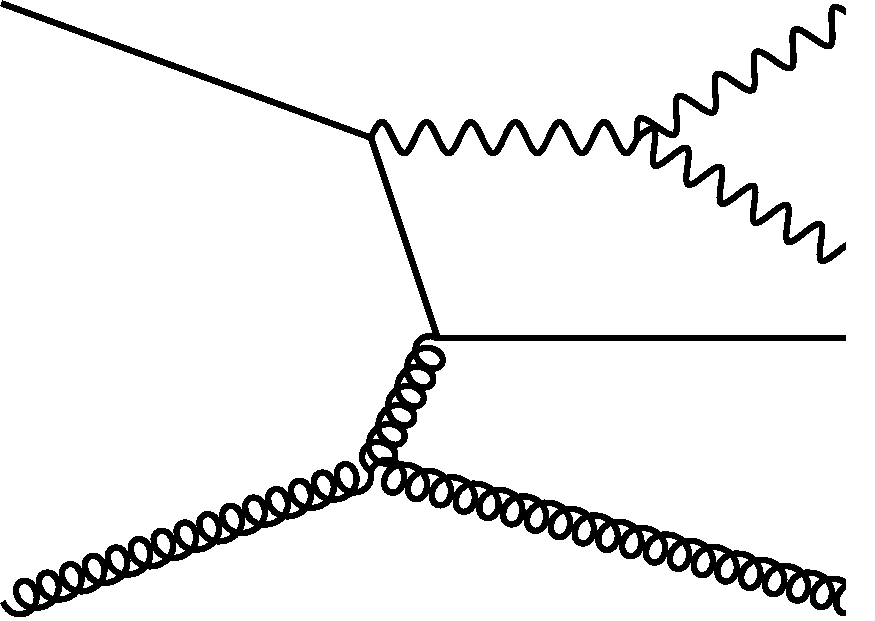
\includegraphics[width=0.3\textwidth]{figures/samples/feynQCD5.pdf}}\\
\subfloat[]{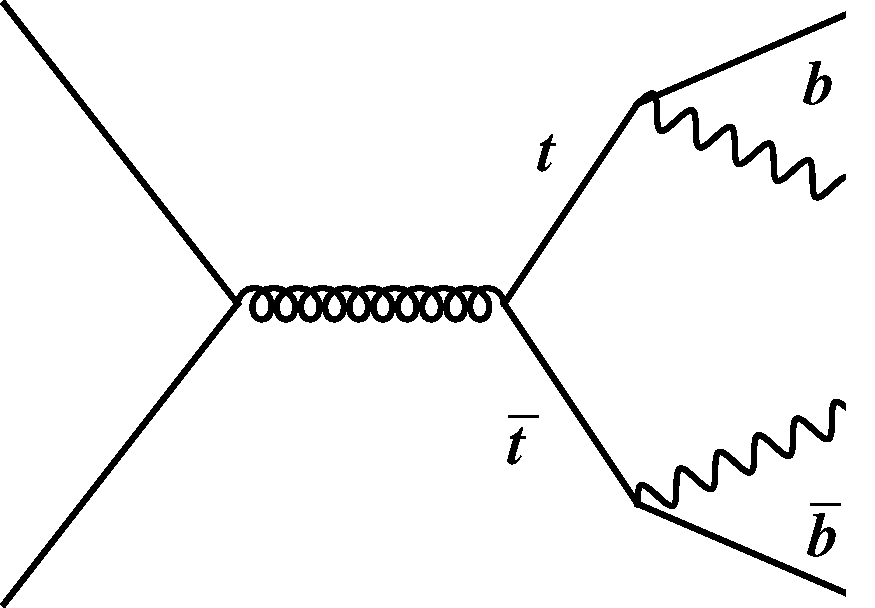
\includegraphics[width=0.3\textwidth]{figures/samples/feynQCD1.pdf}}
\subfloat[]{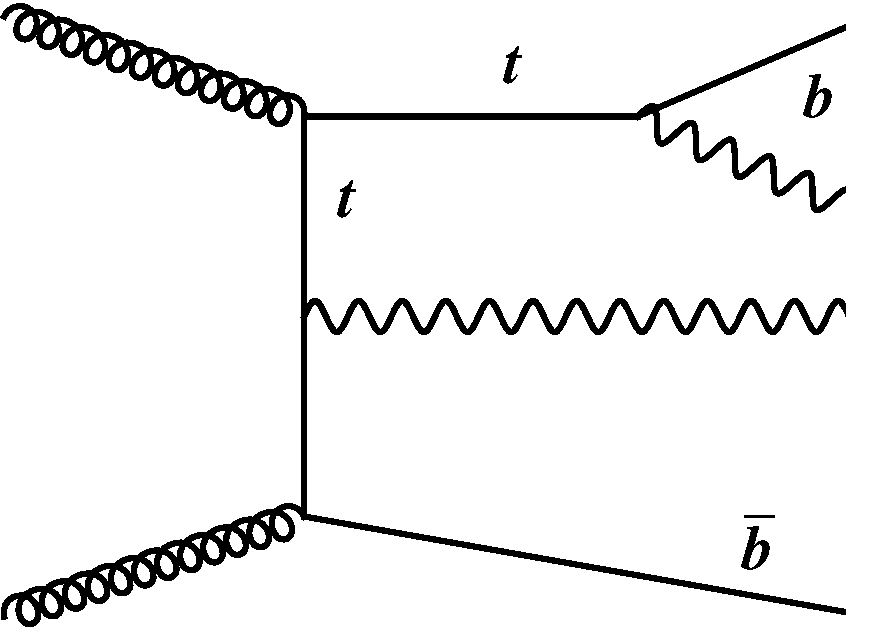
\includegraphics[width=0.3\textwidth]{figures/samples/feynQCD2.pdf}}
\caption{
Examples of $\mathcal{O}(\alpha_{EW}^4 \alpha_{S}^2)$ diagrams that lead to the $VV$+2 parton final state. 
}
\label{fig:feynmanQCD}
\end{center}
\end{figure}

\clearpage
\subsubsection{Signal aQGC processes}
\label{subsec:agc_sample}

As discussed in Section~\ref{Anomalous_Quartic_Gauge_Couplings}, the Eboli model is used to model potential aQGC effects in the VBS process. This model includes 21 D-8 operators, 19 of which can alter the semileptonic VBS final state.
The matrix element for a SM process, incorporating new contributions from EFT, can be expressed as follows:
\begin{equation}
  |A_{\text{SM}} + c_i A_i|^2 = |A_{\text{SM}}|^2 + \sum\limits_i c_i^2 |A_i|^2 + \sum\limits_i 2 c_i \mathrm{Re}(A_{\text{SM}}^\star A_i) + \sum\limits_{i \neq j} c_i c_j \mathrm{Re}(A_i^\star A_j)
\end{equation}
Here, $|A_{\text{SM}}|^2$ denotes the squared matrix element for the SM process, $|A_i|^2$ represents the squared matrix element for pure EFT contributions, $2 \mathrm{Re}(A_{\text{SM}}^\star A_i)$ is the interference between the SM and EFT contributions, and $\mathrm{Re}(A_i^\star A_j)$ is the interference among different EFT contributions. This formulation allows for a detailed breakdown of the process, which can be useful with the matrix-element decomposition method available in recent versions of MadGraph5\_aMC@NLO, enabling the specific generation of each term individually.

To model the Eboli D-8 EFT processes, we generate a series of samples for each operator \(A_i\) at varying coefficient values (\(c_i\)). We utilize MadGraph5\_aMC@NLO version 2.7.2 for these simulations at leading order (LO), incorporating the NNPDF30LO parton distribution function (PDF) set~\cite{Ball:2012cx}, and Pythia 8.244~\cite{Sjostrand:2007gs} for fragmentation processes. The matrix element calculation results in two on-shell \(W/Z\) bosons, which are subsequently decayed using \textsc{MadSpin}~\cite{Artoisenet:2012st} to represent the leptonic and hadronic decay channels. Due to the matrix-element weighting requirements, simulations for each weak isospin state of the boson (e.g., \(W^+W^-\), \(W^+W^+\), \(W^-W^-\), \(W^+Z\), \(W^-Z\), \(ZZ\)) are conducted separately.


\section{Derivation and CxAOD framework}
\label{subsec:DxAOD_and_CxAOD}
%Some technical details on the derivations and analysis framework are described in this section.
For the 1-lepton analysis, we employ the \texttt{HIGG5D2} derivation, which is produced by Athena's derivation framework. This framework consists of tools, algorithms, and Python scripts designed to produce analysis data formats known as derived AODs (DAODs), essential for initiating most analyses. 
DAODs streamline the analysis process by providing a refined dataset, having undergone preliminary selection cuts to minimize data size. These initial cuts are listed in Table~\ref{tab:presel_DxAOD}. Typically, DAODs are generated by a central production team, meaning individual researchers usually engage with the framework directly only for testing purposes on a smaller scale.

\begin{table}[t]
\caption{Pre-selections in the derivation framework for data size reduction. 
$N_j$, $N_J^{\textrm{TCC}}$, and $N_J^{\textrm{LCTopo}}$ represent the counts of different types of jets.} 
\label{tab:presel_DxAOD}
\begin{center}
\resizebox{0.7\textwidth}{!}{
\begin{tabular}{|l|c|}
\hline
\multicolumn{2}{|c|}{ HIGG5D2 ($\ell\nu qq$) } \\
\hline
Trigger & \textit{OR} of all single-lepton and \met triggers \\
\hline
Number of leptons   & $\geq 1$ \\
\hspace{1cm}(lepton \pt)        & $> 20\,\GeV$ \\
\hspace{1cm}(electron quality) & \texttt{DFCommonLHLoose} \\
\hspace{1cm}(muon quality)      & \texttt{DFCommonGoodMuon} \\
\hline
Number of jets      & $N_j \geq 1$ or $N_J^{\textrm{TCC}} + N_{J}^{\textrm{LCTopo}} \geq 1$ \\
\hline
\end{tabular}
}
\end{center}
\end{table}

We use the common analysis \texttt{CxAOD} framework (version \texttt{r33-12}) for this analysis.
The \texttt{CxAOD} framework is used to define physics objects, adhere to all CP recommendations for them, and apply pre-selection cuts.
These procedures and definitions are detailed in Sections~\ref{chap:objects_def} and \ref{subsec:event_preselection}, respectively.
The CP recommendations are providede by the combined performance (CP) groups for use in analysis.

%\section{Data Samples}
%\section{Monte Carlo Samples}
%\section{Derivation and CxAOD Framework}

\chapter{Object Definition}
%%% ObjectDefinition %%%
\label{chap:objects_def}
%This section describes the definitions of the physics objects employed in the analysis (electron, muon, jets and missing transverse energy).
This section describes the definitions of the physics objects used in the analysis.
%We have updated some criteria with respect to the previous analysis:
%
%   \begin{itemize}
%        \item isolation requirements for both electrons/muons
%        \item small-R jets collections (EMTopo $\rightarrow$ PFlow)
%        \item boson tagger for large-R jets tagging (2Var $\rightarrow$ 3Var tagger)
%        \item b-tagging (MV2 $\rightarrow$ DL1r)
%        \item adding fJVT selection
%   \end{itemize}

\section{Electron Definition}
%\subsection{Electron selection}
\label{subsec:electron_selection}
Electron candidates for the analysis were chosen based on specific selection criteria, primarily focusing on their momentum and isolation from surrounding detector activity to identify signal electrons effectively. Electrons traversing the calorimeter's crack were excluded. 
In this 1-lepton channel analysis, exactly one signal electron is required. Electrons failing to meet basic quality standards during data collection are excluded.
The criteria for electron isolation are optimized to reduce the presence of non-prompt electrons.
This analysis uses two electron definitions, Tight and Loose, summarized in Table~\ref{tab:electron_selection}.
%Two distinct electron definitions are used in this analysis.
\begin{itemize}
\item ``Tight'' electron: used to select $W\to e \nu$ candidate.
\item ``Loose'' electron: used to veto events with additional leptons.
\end{itemize}

%In 1-lepton channel, the electron isolation working points are optimized to minimize the contribution of the non-prompt electrons.
%The definitions of the Tight and Loose electrons are summarized in Table~\ref{tab:electron_selection}.

\begin{table}[ht]
\caption{Summary of Electron Selections}
\label{tab:electron_selection}
\resizebox{\textwidth}{!}{
\begin{tabular}[ht]{|c|c|c|c|}
  \hline
  \emph{criteria} & \emph{Loose} & \emph{Tight}\\
  \hline
%  \hline
%  Pseudorapidity range & \multicolumn{2}{c|}{$|\eta| < 2.47$} & $(|\eta| < 1.37) \quad || \quad (1.52 < |\eta| < 2.47)$ \\
  Pseudorapidity range & \multicolumn{2}{c|}{$|\eta| < 2.47$ (veto in [1.37, 1.52] region)} \\
  \hline
  Energy calibration & \multicolumn{2}{c|}{``es2017\_R21\_v0'' (ESModel)}\\
  \hline
  Transverse momentum & $\pt > 7\,\GeV$ & $\pt > 28~\GeV$ \\
  \hline
  \multirow{2}{*}{Object quality~\cite{twiki_egQual}} & \multicolumn{2}{c|}{Not from a bad calorimeter cluster (BADCLUSELECTRON)} \\ \cline{2-3}
  & \multicolumn{2}{c|}{Remove clusters from regions with EMEC bad HV (2016 data only)} \\
  \hline
  \multirow{2}{*}{Track to vertex association} & \multicolumn{2}{c|}{$|d_{0}^{BL}(\sigma)|$ $<$ 5} \\ \cline{2-3}
  & \multicolumn{2}{c|}{$|\Delta z_{0}^{BL} \sin{\theta}| <$ 0.5~mm} \\
  \hline
  Identification & Loose & Tight \\
  \hline
            %& LooseTrackOnly & \\
  Isolation &  FCLoose at $\pt<100\,\GeV$                   &  FixedCutHighPtCaloOnly \\
            &  and no isolation requirement at $>100\,\GeV$ & \\
  \hline
 \end{tabular}}
\end{table}

\vspace{1cm}

%Notes:
%\begin{itemize}
% \item Electron ID: 3 working points (Loose/Medium/Tight) are evaluated using the Likelihood-based (LH) method, by the
% \mbox{\texttt{\href{https://twiki.cern.ch/twiki/bin/view/AtlasProtected/EGammaIdentificationRun2}{ElectronPhotonSelectorTools}}}.
%\item Energy calibration of electrons is implemented in the\\
%  \mbox{\texttt{\href{https://twiki.cern.ch/twiki/bin/view/AtlasProtected/ElectronPhotonFourMomentumCorrection}{ElectronPhotonFourMomentumCorrection}}} tool.
%\item Scale Factors for efficiencies for electrons are implemented in the\\
%  \mbox{\texttt{\href{https://twiki.cern.ch/twiki/bin/view/AtlasProtected/XAODElectronEfficiencyCorrectionTool}{ElectronEfficiencyCorrection}}} tool.
%\item Updated configurations for the EGamma CP tools can be found on this \mbox{\texttt{\href{https://twiki.cern.ch/twiki/bin/view/AtlasProtected/EGammaRecommendationsR21}{twiki}}} page.
%\end{itemize}

%%%Electron ID working points are evaluated using the Likelihood-based (LH) method, by the 
%%%\mbox{\texttt{\href{https://twiki.cern.ch/twiki/bin/view/AtlasProtected/EGammaIdentificationRun2}{ElectronPhotonSelectorTools}}}
%%%;
%%%energy calibration of electrons is implemented in the\\
%%% \mbox{\texttt{\href{https://twiki.cern.ch/twiki/bin/view/AtlasProtected/ElectronPhotonFourMomentumCorrection}{ElectronPhotonFourMomentumCorrection}}} tool
%%%;
%%%Scale Factors for efficiencies for electrons are implemented in the\\
%%% \mbox{\texttt{\href{https://twiki.cern.ch/twiki/bin/view/AtlasProtected/XAODElectronEfficiencyCorrectionTool}{ElectronEfficiencyCorrection}}} tool.

%\newpage

\section{Muon Definition}
%\subsection{Muon selection}
\label{subsec:muon_selection}
Muons are chosen similarly to electrons, with the key distinction being the use of the muon spectrometer instead of the calorimeter. They must meet comparable momentum and isolation criteria, plus a consistency check aligning tracks from the inner detector to the muon spectrometer. Muons failing basic quality standards during data collection are excluded.
The criteria for muon identification and isolation are optimized to reduce the presence of non-prompt muons.
This analysis uses two muon definitions, Tight and Loose, summarized in Table~\ref{tab:muon_selection}.
%Two types of muon definitions are used in this analysis.
\begin{itemize}
\item ``Tight'' muon: used to select $W\to \mu\nu$ candidate.
\item ``Loose'' muon: used to veto events with additional leptons.
\end{itemize}
%In 1-lepton channel, the muon identification and isolation working points are optimized to minimize the contributions of the non-prompt muon.
%The definitions of the Tight and Loose muons are summarized in Table~\ref{tab:muon_selection}.

\begin{table}[ht]
\caption{Summary of Muon Selections}
\label{tab:muon_selection}
\begin{center}
%\resizebox{\textwidth}{!}{
\begin{tabular}[ht]{|c|c|c|}
\hline
  \emph{Criteria} & \emph{Loose} & \emph{Tight}\\
\hline
  Pseudorapidity range & \multicolumn{2}{c|}{$|\eta|<2.5$} \\
\hline
  Momentum Calibration & \multicolumn{2}{c|}{Sagitta Correction Used} \\
\hline
  Transverse momentum & $\pt > 7~\GeV$ & $\pt > 28~\GeV$ \\
\hline
  $d_0$ Significance Cut & \multicolumn{2}{c|}{$|d_{0}^{BL}(\sigma)|<3$} \\
\hline
  $z_0$ Cut & \multicolumn{2}{c|}{$|z_{0}^{BL} \sin\theta| < 0.5$~mm} \\
\hline
  Selection Working Point & Loose & Medium\\
\hline
                          %& LooseTrackOnly & \\
  Isolation Working Point & FCLoose at $\pt<100\,\GeV$                   & FixedCutTightTrackOnly \\
                          & and no isolation requirement at $>100\,\GeV$ & \\
\hline
\end{tabular}
%}
\end{center}
\end{table}

%Notes: 
%The selection criteria are implemented in the MuonSelectorTools with MuonMomentumCorrections, isolation in IsolationSelection and $d_0$ and $z_0$ cuts in xAODTracking packages.   
%The muon recommendations can be found here: \mbox{\texttt{\href{https://twiki.cern.ch/twiki/bin/view/AtlasProtected/MCPAnalysisConsolidationMC16}{MCPAnalysisConsolidationMC16}}}.

%\newpage

\section{Jet Definitions}
In particle accelerator experiments, detecting quarks is challenging due to quark confinement.
Since the strong nuclear force prevents their isolation, quarks undergo hadronization when they are separated.
As the energy in the strong field between separating quarks increases, a new quark-antiquark pair will eventually be created from the vacuum.
These newly formed quarks then combine with the original quarks to form more hadrons.
If the original quarks have high enough momentum, this process will repeat and lead to a shower of hadrons observed in the detector. Using clustering algorithms, these hadronic showers can be reconstructed as a cone-shaped energy pattern, known as a jet.

\subsection{Small-R jet selection}
\label{subsec:jet_selection}

When a heavy particle decays, it can produce two quarks that rapidly move away from each other and form two distinct jets of particles, observable in detectors. If the original particle is moving slowly, it results in two compact, easily distinguishable jets.
These compact jets are referred to as Small-R jets, characterized by their small radius.

Small-R jets are used for reconctructing the less boosted $W/Z \to qq$ candidates, delineating \(qq\) pairs from \(V\) boson decays as ``Signal'' jets and forward jets in vector-boson scattering (``VBS'' jets). Sections \ref{subsec:vbs_selection} and \ref{subsubsec:merged_jets_selection}-\ref{subsubsec:resolved_jets_selection} provide in-depth discussions on Signal and VBS jets. We use the ATLAS baseline jet reconstruction algorithm, the \texttt{AntiKt4EMPFlowJets}, which is anti-$k_t$ clustering algorithm.
Standard jet calibrations are implemented, including the use of Jet Vertex Tagging (JVT) with a Medium Working Point (WP) to reduce pile-up interactions. 
To further suppress pile-up jets, especially in the forward-like topology relevant to our analysis, the forward-JetVertexTagger (fJVT) is applied, enhancing the focus on jets from the targeted VBS-scattering processes.
Small-R jet selection criteria is summarized in Table~\ref{tab:small_R_jet_summary}.
%%%%%
%%Small-R jets are used to reconstruct $W/Z \to qq$ candidates that are less boosted so that the $qq$ pair
%%from the $V$ boson decay are well separated (``Signal'' jets), and to select the forward jets coming from vector-boson scattering (``VBS''
%%jets); both Signal and VBS jets definitions will be discussed in details in sections \ref{subsec:vbs_selection} and \ref{subsubsec:merged_jets_selection}-\ref{subsubsec:resolved_jets_selection} respectively.
%%The ATLAS baseline reconstruction algorithm is used (\texttt{AntiKt4EMPFlowJets}).
%%
%%Usual calibrations are applied to the jets. 
%%The Jet Vertex Tagging (JVT) with Medium WP is applied to the jets to suppress pile-up interactions.
%%Furthermore, BadBatMan flag cleaning is turned on in the analysis framework to remove the BatMan effect.
%%
%%In the context of the pile-up jets suppression, 
%%forward-JetVertexTagger (fJVT) has been introduced in this round of the analysis 
%%to mitigate the jet candidates contributions coming from pile-up interaction 
%%rather than the hard processes we are targeting. 
%%This is motivated mainly by the forward-like topology we are interested in. 

%In particular, Loose WP is used, as described in section \ref{subsec:vbs_selection}, 
%and recommendation are followed from the internal twiki 
%\mbox{\texttt{\href{https://twiki.cern.ch/twiki/bin/view/AtlasProtected/PileupJetRecommendations}{fJVT}}}.


%Small-R jet selection criteria is summarized in Table~\ref{tab:small_R_jet_summary}.

\begin{table}[ht]
\caption{Summary of small-R jet selection and calibration}
\label{tab:small_R_jet_summary}
\resizebox{\textwidth}{!}{
\begin{tabular}{|c|c|c|}
\hline
%\large
\multicolumn{3}{|c|}{Jet reconstruction parameters} \\
%\normalsize
\hline
Parameter & \multicolumn{2}{c|}{Value} \\ 
\hline
algorithm & \multicolumn{2}{c|}{anti-k$_\text{T}$}  \\
R-parameter & \multicolumn{2}{c|}{0.4} \\
input constituent & \multicolumn{2}{c|}{EMPFlow} \\
Analysis Release Number &\multicolumn{2}{c|}{ 21.2.164 } \\
CalibArea tag & \multicolumn{2}{c|}{00-04-82} \\
Calibration configuration & \multicolumn{2}{c|}{JES\_MC16Recommendation\_Consolidated\_PFlow\_Apr2019\_Rel21.config} \\
Calibration sequence (Data) & \multicolumn{2}{c|}{JetArea\_Residual\_EtaJES\_GSC\_Insitu} \\
Calibration sequence (MC) & \multicolumn{2}{c|}{JetArea\_Residual\_EtaJES\_GSC\_Smear} \\
%Calibration sequence (AFII) & JetArea\_Residual\_EtaJES\_GSC \\
\hline
%\large
\multicolumn{3}{|c|}{Selection requirements} \\
%\normalsize
\hline
%& \textbf{``Signal'' jet} & \textbf{``VBS'' jet} \\
%\hline
Observable & \multicolumn{2}{c|}{Requirement} \\
\hline
Jet cleaning & \multicolumn{2}{c|}{LooseBad} \\
\hline
BatMan cleaning & \multicolumn{2}{c|}{Yes} \\
\hline
\pt                         & \multicolumn{2}{c|}{$>$20~GeV ($|\eta|<2.5$) and $>$30~GeV ($2.5<|\eta|<4.5$)}   \\
\hline
\textbar$\eta$\textbar      & \multicolumn{2}{c|}{$<4.5$} \\
\hline
JVT & \multicolumn{2}{c|}{$>0.5$ for 60 GeV$<\pt<$120~GeV and $\left|\eta\right|<2.4$ } \\
WP  & \multicolumn{2}{c|}{Medium} \\
Config  & \multicolumn{2}{c|}{Moriond2018/JvtSFFile\_EMPFlow.root} \\
\hline
fJVT & \multicolumn{2}{c|}{$>0.5$ (and $|timing|<10 \ ns$)} \\
     & \multicolumn{2}{c|}{for $\pt<$120~GeV and $2.5 < \left|\eta\right|<4.5$}  \\
WP   & \multicolumn{2}{c|}{Loose} \\
Config  & \multicolumn{2}{c|}{Moriond2018/fJvtSFFile.root} \\
\hline
$b$-tagging (See Sec.~\ref{subsec:flavortagging}) & \multicolumn{2}{c|}{Tagged, or not tagged} \\
\hline
\end{tabular}}
\end{table}






\clearpage
\subsection{Large-R jet selection}
\label{subsec:large-Rjet}
For high-\pt $W/Z \to qq$ candidates, the angle between the two jets narrows, leading to the merging of jets. Clustering algorithms then reconstruct them into a single, larger-radius jet, known as a large-R jet, which encompasses the two merged sub-jets.
Following the trimming procedure\cite{Krohn:2009th} to reduce pile-up and soft radiation effects, the ``jet mass'', $m_J$, 
is reconstructed by summing the four-vectors of jet constituents, treated as massless. The large-R jets then undergo baseline kinematic cuts as prescribed by the CP group:

        \begin{itemize}
                \item $\pt^{J} > 200 \, \GeV$
                \item $|\eta|^{J} < 2$
                \item $m^{J} > 50 \, \GeV$
        \end{itemize}

The (large-R) jet substructure variable, $D_{2}$, derived from the energy correlation functions based on energies and pair-wise angles of the sub-constituents\cite{Larkoski:2014gra,Larkoski:2015kga}, is sensitive to the expected 2-prong sub-structure from the boosted W/Z bosons decay. The variable $D_{2}$ is defined as
\begin{equation}
D^{(\beta=1)}_2 = E_{CF3} \left( \frac{E_{CF1}}{E_{CF2}} \right)^3 \\
\end{equation}
where the energy correlation functions ($E_{CF}$) are defined as:
\begin{equation}
\begin{split}
E_{CF1} = \sum_{i} p_{T,i}
\\
E_{CF2} = \sum_{ij} p_{T,i}p_{T,j} \Delta R_{ij}
\\
E_{CF3} = \sum_{ijk} p_{T,i}p_{T,j}p_{T,k} \Delta R_{ij} \Delta R_{jk} \Delta R_{ki}
\end{split}
\end{equation}

The track multiplicity, $n_{\text{Tracks}}$, of the ungroomed large-R jet is also used to enhance background rejection. It is particularly sensitive to QCD jets from single-quark and gluon decays. 
%The utilization of these variables in defining the merged category is detailed in Section~\ref{subsubsec:merged_jets_selection}.
The $W/Z$ boson tagger, based on three variables—$m_J$, $D_{2}$, $n_{\text{Tracks}}$—is used to identify boson jets from large-R jet candidates. The application of this tagger and the three variables in defining the merged category is elaborated in Section~\ref{subsubsec:merged_jets_selection}.

%%%
%%%Large-R jet (\texttt{AntiKt10LCTopoTrimmedPtFrac5SmallR20})
%%%is used to reconstruct high-\pt $W/Z \to qq$ candidates.
%%%After the trimming procedure\cite{Krohn:2009th} to suppress the pileup and soft radiations, the ``jet mass'', $m_J$, is reconstructed by the four-vector sum of the jet constituents, assuming they are massless particles.
%%%The reconstructed $m_J$ peaks around the $m_{W/Z}$ for $W/Z \to q\bar{q}$ signals and distributes broadly for single-quark- and gluon-induced jets (see Section~\ref{subsubsec:merged_jets_selection}).
%%%
%%%Baseline kinematics cuts are applyied on the large-R jets collection as CP group prescriptions:
%%%
%%%        \begin{itemize}
%%%                \item $\pt^{J} > 200 \, \GeV$
%%%                \item $|\eta|^{J} < 2$
%%%                \item $m^{J} > 50 \, \GeV$
%%%        \end{itemize}
%%%
%%%In addition to the window cut on the jet mass distribution, we use the jet substructure variable, $D_{2}$, reconstructed by the energy correlation functions based on energies and pair-wise angles of the sub-constituents\cite{Larkoski:2014gra,Larkoski:2015kga}. The variable $D_{2}$ is defined as
%%%\begin{equation}
%%%D^{(\beta=1)}_2 = E_{CF3} \left( \frac{E_{CF1}}{E_{CF2}} \right)^3 \\
%%%\end{equation}
%%%where the energy correlation functions ($E_{CF}$) are defined as:
%%%\begin{equation}
%%%\begin{split}
%%%E_{CF1} = \sum_{i} p_{T,i}
%%%\\
%%%E_{CF2} = \sum_{ij} p_{T,i}p_{T,j} \Delta R_{ij}
%%%\\
%%%E_{CF3} = \sum_{ijk} p_{T,i}p_{T,j}p_{T,k} \Delta R_{ij} \Delta R_{jk} \Delta R_{ki}
%%%\end{split}
%%%\end{equation}
%%%
%%%The $D_{2}$ variable is sensitive to the 2-prong sub-structure we expect from the W/Z bosons decay; 
%%%furthermore, we use the track multiplicity of the large-R jet to improve the background rejection, 
%%%indeed, this variable is more sensitive to the single-quark or -gluon decay of QCD jets; 
%%%in particular, tracks with standard reconstruction criteria and \pt $> 500 \ MeV$ associated to the un-groomed large-R jet
%%%are used in the calculation.


%%\textbf{Optimization of $W/Z$-tagging}
%%
%%We use the central boson tagger recommendation to identify our large-R jet candidates as W/Z boson jets and 
%%to reject the other SM background processes (mainly, V+jets and $t\bar{t}$ after the analysis pre-selection). 
%%In particular, we use the 3-variables based tagger, that relies on the sub-structure variables, $D_2$ and $nTracks$, 
%%as well as the jet mass; two central fixed efficiency WPs are provided (50\% and 80\%). 
%%Dedicated optimization studies available from the JetEtMiss group are available here:
%%\mbox{\texttt{\href{https://indico.cern.ch/event/806078/contributions/3354584/attachments/1812138/2960029/JSS_14mar2019.pdf}{OptimisationStudies}}}.

%More info are available on the central reccomendation page 
%\mbox{\texttt{\href{
%https://twiki.cern.ch/twiki/bin/viewauth/AtlasProtected/BoostedJetTaggingRecommendationFullRun2
%}
%{BoostedJetTaggingRecommendationFullRun2}
%}}
%as well as the dedictaed optimisation studies can be found here 
%\mbox{\texttt{\href{
%https://indico.cern.ch/event/806078/contributions/3354584/attachments/1812138/2960029/JSS_14mar2019.pdf
%}
%{OptimisationStudies}
%}}.


%%%Boson tagging efficiency scale factors~(SF) are applied to simulated events. 
%%%The boson tagging efficiency SF and the uncertainty
%%%are estimated using dedicated data samples according to JetTagging recommendations.
%%%%the central JetTagging recommendations
%%%%\mbox{\texttt{\href{
%%%%https://twiki.cern.ch/twiki/bin/view/AtlasProtected/JetUncertaintiesRel21ConsolidatedLargeRTaggerSF
%%%%}
%%%%{JetUncertaintiesRel21ConsolidatedLargeRTaggerSF}
%%%%}}.
%%%In particular, central boson tagger SF are not available only for the exclusive (80\%-50\%) region, 
%%%but an additional derivation has been done in the phase space of the analysis as recommended by the JetTagging group; 
%%%details are provided in appendix \ref{app:LP_SF}.

Summary of selections and calibrations of the large-R jet is shown in Table~\ref{tab:largeR_jet_summary}.


\begin{table}[ht]
\caption{Summary of large-R jet selections and calibrations}
\label{tab:largeR_jet_summary}
\resizebox{\textwidth}{!}{
\begin{tabular}{|c|c|}
\hline
%\large
\multicolumn{2}{|c|}{Jet reconstruction parameters} \\
\hline
%\normalsize
Parameter & Value \\ 
\hline
algorithm & anti-k$_{T}$  \\
R-parameter & 1.0 \\
input constituent & LCTopoCluster \\
grooming algorithm & Trimming \\ 
$f_{cut}$ & 0.05 \\
$R_{trim}$ & 0.2 \\
Analysis Release Number & 21.2.164 \\
%Calibration tag & JetCalibTools-00-04-76 \\
%CalibArea tag & 00-04-81 \\
Calibration configuration (Data) & JES\_MC16recommendation\_FatJet\_Trimmed\_JMS\_comb\_March2021.config \\
Calibration configuration (MC) & JES\_MC16recommendation\_FatJet\_Trimmed\_JMS\_comb\_17Oct2018.config \\
Calibration sequence (Data) & EtaJES\_JMS\_Insitu\_InsituCombinedMass \\
Calibration sequence (MC) & EtaJES\_JMS \\
\hline
%\large
\multicolumn{2}{|c|}{Selection requirements} \\
%\normalsize
\hline
Observable & Requirement \\
\hline
\pt  & $>$200 GeV \\
\textbar$\eta$\textbar & $<$2.0 \\
mass & $>$ 50~GeV \\
\hline
\multicolumn{2}{|c|}{SmoothedWZTagger} \\\hline
Object  & Working point \\\hline
$W$/$Z$ & 3-var tagger working point \\
%$Z\rightarrow bb$ & single/double b-tag with/without loose/tight mass \\\hline
        & \texttt{SmoothedContainedVTagger\_AntiKt10LCTopoTrimmed\_FixedSignalEfficiencyXX\_MC16\_20201216.dat} \\
        & with V = {W, Z} and XX = {50, 80} \\
\hline
\end{tabular}}
\end{table}


%%Move to its own tex file

%%%\subsection{MET reconstruction}
%%%Missing transverse energy, \MET , is the total energy of all the undetected particles in an event. In this analysis, with just one neutrino in the final state, it’s assumed that the \MET directly corresponds to this single neutrino’s energy. The \MET reconstruction is done based on the signals of detected particles in the final state.
%%%\begin{equation}
%%%\label{eq:METformula}
%%%E_{x(y)}^{\text{miss}} = E_{x(y)}^{\text{miss}, e} + E_{x(y)}^{\text{miss}, \gamma} + E_{x(y)}^{\text{miss}, \tau} + E_{x(y)}^{\text{miss, jets}} + E_{x(y)}^{\text{miss}, \mu} + E_{x(y)}^{\text{miss, soft}}
%%%\end{equation}
%%%
%%%After the calibrations for pileup, two types of contributions are taken into account in the reconstruction.
%%%        \begin{itemize}
%%%                \item hard-event signals: fully reconstructed and calibrated particles ($e, \gamma, \tau, \mu$) and small-R jets
%%%                \item soft-event signals: soft tracks in the inner detector not parts of any reconstructed physical object 
%%%        \end{itemize}
%%%When taking the negative vectorial sum of all contributing physics objects, only the calorimeter signals are used to avoid double counting~\cite{PERF-2016-07}.

%%%Missing transverse energy, $E_{\text{T}}^{\text{miss}}$, is reconstructed by taking the negative vectorial sum of all the reconstructed and calibrated 
%%%electrons, muons, and small-R jets, after the calibrations have accounted for pileup:
%%%\begin{equation}
%%%\label{eq:METformula}
%%%E_{x(y)}^{\text{miss}} = E_{x(y)}^{\text{miss}, e} + E_{x(y)}^{\text{miss}, \gamma} + E_{x(y)}^{\text{miss}, \tau} + E_{x(y)}^{\text{miss, jets}} + E_{x(y)}^{\text{miss}, \mu} + E_{x(y)}^{\text{miss, soft}}
%%%\end{equation}
%%%
%%%For all of these physics objects used to reconstruct $E_{\text{T}}^{\text{miss}}$, only the calorimeter signals are used. 
%%%Large-R jets are not included in this definition to avoid double counting with small-R jets, and a ``soft term'' is used to account 
%%%for soft radiation terms that leave tracks in the inner detector but are not used in any reconstruction of physics objects~\cite{PERF-2016-07}.
%%%
%%%In this note, the term $p_{T}^{\text{miss}}$ is also used. For the purpose of this note, $p_{T}^{\text{miss}}$ means the vectorial sum of 
%%%transverse momenta reconstructed from particle tracks, and is used interchageably with the term $p_{track}$. This $p_{T}^{\text{miss}}$ term
%%%is used together with $E_{\text{T}}^{\text{miss}}$ to set MET requirements in the event selection. 

%%\subsection{Jet flavor tagging selection}
\label{subsec:flavortagging}

Due to the short lifetime of the $t$ quark, it decays before hadronization, with a $99.8\%$ chance of decaying into a $b$ quark. 
As a result, a $b$-tagging method is used to reject events originating from \ttbar 
and single top events. 
In this analysis, small-R jets are tagged using the new DL1r $b$-tagging score available in ATLAS~\cite{FTAG-2018-01}.
The DL1r $b$-tagging is based on a deep-learning neural network using distinctive features of b-hadrons~\cite{Aad2023flavour}.
As specified in Section~\ref{subsec:cr_selection}, the b-tagged jets are used to define the TopCR within the \olep phase space.
A summary of the $b$-tagging requirements in the resolved category is shown in Table~\ref{tab:b_tag_resolved}.

\begin{table}[ht]
\begin{center}
\caption{Summary of $b$-tag requirements in the resolved category}
\label{tab:b_tag_resolved}
\begin{tabular}{|l|c|}\hline
Jet collection          & AntiKt4PFlowJets \\\hline
Jet selection           & ``Signal jet'' and ``VBS jet'' selection in Table~\ref{tab:small_R_jet_summary}    \\
                 \hline
Algorithm               & DL1r        \\\hline
Operating Point      & Fixed, Efficiency = 70\% \\\hline
%CDI                & 2020-21-13TeV-MC16-CDI-2020-03-11\_v3 \\
%\hline
\end{tabular}
\end{center}
\end{table}%


\clearpage
\section{Missing Energy Definition}
%\subsection{MET reconstruction}
\label{sec:MET_reconstruction}
%In the ATLAS experiment, missing transverse energy (MET) represents the total energy of particles not detected, typically neutrinos. In analyses with just one neutrino in the final state, it's assumed that the MET directly corresponds to this single neutrino's energy. 
Missing transverse energy, \MET , is the total energy of all the undetected particles in an event. In this analysis, with just one neutrino in the final state, it’s assumed that the \MET directly corresponds to this single neutrino’s energy. The \MET reconstruction is done based on the signals of detected particles in the final state.
%The MET reconstruction is done based on the signals of detected particles in the final state.
\begin{equation}
\label{eq:METformula}
E_{x(y)}^{\text{miss}} = E_{x(y)}^{\text{miss}, e} + E_{x(y)}^{\text{miss}, \gamma} + E_{x(y)}^{\text{miss}, \tau} + E_{x(y)}^{\text{miss, jets}} + E_{x(y)}^{\text{miss}, \mu} + E_{x(y)}^{\text{miss, soft}}
\end{equation}

After the calibrations for pileup, two types of contributions are taken into account in the reconstruction.
        \begin{itemize}
                \item hard-event signals: fully reconstructed and calibrated particles ($e, \gamma, \tau, \mu$) and small-R jets
                \item soft-event signals: soft tracks in the inner detector not parts of any reconstructed physical object 
        \end{itemize}
%fully reconstructed and calibrated particles($e, \gamma, \tau, \mu$) and small-R jets
When taking the negative vectorial sum of all contributing physics objects, only the calorimeter signals are used to avoid double counting~\cite{PERF-2016-07}.

%%%Missing transverse energy, $E_{\text{T}}^{\text{miss}}$, is reconstructed by taking the negative vectorial sum of all the reconstructed and calibrated 
%%%electrons, muons, and small-R jets, after the calibrations have accounted for pileup:
%%%\begin{equation}
%%%\label{eq:METformula}
%%%E_{x(y)}^{\text{miss}} = E_{x(y)}^{\text{miss}, e} + E_{x(y)}^{\text{miss}, \gamma} + E_{x(y)}^{\text{miss}, \tau} + E_{x(y)}^{\text{miss, jets}} + E_{x(y)}^{\text{miss}, \mu} + E_{x(y)}^{\text{miss, soft}}
%%%\end{equation}
%%%
%%%For all of these physics objects used to reconstruct $E_{\text{T}}^{\text{miss}}$, only the calorimeter signals are used. 
%%%Large-R jets are not included in this definition to avoid double counting with small-R jets, and a ``soft term'' is used to account 
%%%for soft radiation terms that leave tracks in the inner detector but are not used in any reconstruction of physics objects~\cite{PERF-2016-07}.
%%%
%%%In this note, the term $p_{T}^{\text{miss}}$ is also used. For the purpose of this note, $p_{T}^{\text{miss}}$ means the vectorial sum of 
%%%transverse momenta reconstructed from particle tracks, and is used interchageably with the term $p_{track}$. This $p_{T}^{\text{miss}}$ term
%%%is used together with $E_{\text{T}}^{\text{miss}}$ to set MET requirements in the event selection. 

\section{Jet Flavor ($b$) Tagging Definition}
%\subsection{Jet flavor tagging selection}
\label{subsec:flavortagging}

Due to the short lifetime of the $t$ quark, it decays before hadronization, with a $99.8\%$ chance of decaying into a $b$ quark. 
As a result, a $b$-tagging method is used to reject events originating from \ttbar 
and single top events. 
In this analysis, small-R jets are tagged using the new DL1r $b$-tagging score available in ATLAS~\cite{FTAG-2018-01}.
The DL1r $b$-tagging is based on a deep-learning neural network using distinctive features of b-hadrons~\cite{Aad2023flavour}.
As specified in Section~\ref{subsec:cr_selection}, the b-tagged jets are used to define the TopCR within the \olep phase space.
A summary of the $b$-tagging requirements in the resolved category is shown in Table~\ref{tab:b_tag_resolved}.

\begin{table}[ht]
\begin{center}
\caption{Summary of $b$-tag requirements in the resolved category}
\label{tab:b_tag_resolved}
\begin{tabular}{|l|c|}\hline
Jet collection          & AntiKt4PFlowJets \\\hline
Jet selection           & ``Signal jet'' and ``VBS jet'' selection in Table~\ref{tab:small_R_jet_summary}    \\
                 \hline
Algorithm               & DL1r        \\\hline
Operating Point      & Fixed, Efficiency = 70\% \\\hline
%CDI                & 2020-21-13TeV-MC16-CDI-2020-03-11\_v3 \\
%\hline
\end{tabular}
\end{center}
\end{table}%


%\input{src/object_selection/tracks_selection}
%\subsection{fJVT}
\label{subsec:fjvt}

In the context of the pile-up jets suppression, forward-JetVertexTagger (fJVT) has been introduced in this round of the analysis to mitigate the jet candidates contributions coming from pile-up interaction rather than the hard processes we are targeting. This is motivated mainly by the forward-like topology we are interested in. In particular, Loose WP is used, as described in section \ref{subsec:vbs_selection}, and recommendation are followed from the internal twiki \mbox{\texttt{\href{https://twiki.cern.ch/twiki/bin/view/AtlasProtected/PileupJetRecommendations}{fJVT}}}.

\section{Overlap Removal}
%\subsection{Overlap Removal}

We utilize the standard overlap removal tools, AssociationUtils~\cite{Farrell2023AssociationUtils}, to manage the overlaps between analysis-level objects (electrons, muons, jets, etc.). This approach ensures that the same energy deposits are not used in the reconstruction of multiple analysis-level objects. The specific overlap removal tools employed in this analysis are summarized in Table~\ref{tab:OR}.
The overlap between small-R and large-R jets will be addressed in the later stages of the selection process by adopting a ``Merged over Resolved'' regime categorization, as detailed in Sections \ref{subsec:sr_selection} and \ref{subsubsec:merged_jets_selection}.

\begin{table}[ht]
\caption{The sequential application of overlap removal conditions. $\Delta R$ is calculated using rapidity by default.}
\label{tab:OR}
\begin{center}
\small
%\resizebox{\textwidth}{!}{
\begin{tabular}{|c|c|c|}
\hline
 Reject & Against & Criteria \\\hline
 electron & electron & shared track, $p_{T,1} < p_{T,2}$ \\
 muon     & electron & is calo-muon and shared ID track \\
 electron & muon     & shared ID track \\
 jet      & electron & $\Delta R <$ 0.2 \\ %Not a bjet and $\Delta R <$ 0.2] 
 electron & jet      & $\Delta R <$ 0.4 \\
 jet      & muon     & NumTrack $<$ 3 and (ghost-associated or $\Delta R <$ 0.2) \\
 muon     & jet      & $\Delta R <$ min(0.4, 0.04 + $10\,\text{GeV}/p_{T,\mu}$) \\ %$\Delta R <$ 0.4
 large-R-jet  & electron & $\Delta R <$ 1.0 \\
\hline
\end{tabular}
%}
\end{center}
\end{table}




%\section{Electron Definition}
%\section{Muon Definition}
%\section{Jet Definitions}
%\subsection{Small-R Jet Selection}
%\subsection{Large-R Jet Selection}
%\section{Missing Energy Definition}
%\section{Jet Flavor Tagging Definition}
%\section{Overlap Removal}

\chapter{Event Selections}
%%% EventSelection %%%

This section describes the event selection, which has been optimized in order to maximize the expected significance of the signal over background.

A set of preselection cuts are applied first, including basic quality cuts (event cleaning) and  trigger requirements.
Some preselection cuts applied in the \texttt{CxAODMaker} are also summarized.

For the main event selection, first the selection of the $W/Z$ boson decaying leptonically is performed. 
The candidate boson is selected targeting $Z\to \ell\ell$, $W\to \ell\nu$ and $Z\to \nu\nu$, respectively.

Then in each lepton channel, the hadronic part of the final state is considered 
in order to enhance the VBS associated objects and to select the second boson decaying hadronically. 
A usual tagging jets procedure is performed for the VBS-jet candidates selection 
while a hadronically decaying $V$ candidate is identified, 
either reconstructed as a large-$R$ jet (merged regime), or two small-$R$ jets (resolved regime).

In each channel, some topological cuts are applied to suppress the background. 
Cuts are designed to define some analysis SRs, with enhanced sensitivity to the target signal,
and some analysis CRs, with enhanced SM background processes to constraint them in the fit. 
In particular, for events falling in the merged regime the boson tagger is used to define the SRs 
and reverted cut for defining CRs for the \Vjets background; for events in the resolved regime,
a signal di-jets system is built and the invariant mass of it is used to define a mass window (SR) 
or sidebands (CRs for \Vjets). Only in the \olep channel, dedicated TopCR are defined r
equiring additional b-jets in the event.

%The current selection is mainly reproducing what has been optmised in the previous round, 
%except for some dedicated optimisations:

First a summary of all the selections will be provided to give an full overview of it to the reader,
then, the detailed selections will be explained throughout this section. 

During this pass of the analysis, 
we focused on the optimization of the signal jets selection in both resolved and merged regime 
during the R\&D phase of the analysis and introduced new criteria with respect to the early run-2 version of this analysis:

\begin{itemize}
  \item moving signal jets selection ($V \rightarrow qq$ decay products) from close-V algorithm to leading $p_T$ criteria; some studies are showed in appendix \ref{app:res_opt};
  \item moving to latest boson tagger configuration (3-variables instead of the previous 2-variables), details and references to the new tagger are put in section \ref{subsec:large-Rjet};
  \item moving to an inclusive merged CR instead of HighPurity/LowPurity (defined in Section \ref{subsubsec:merged_jets_selection}) CRs in order to take into account recommendation for boson tagger SFs, details are discussed in appendix \ref{app:merged_cr}.
\end{itemize}

The SM EW VV+jj MC samples have been used to check the sensitivity to our target signal process.

% move here after Oldrich comment
\clearpage
\subsection{Summary of the SR and CR selections}
\label{subsec:summary_selection}

The selections applied are summarized here in tables 
\ref{tab:0lep_merged}-\ref{tab:0lep_resolved}
\ref{tab:1lep_merged}-\ref{tab:1lep_resolved}
\ref{tab:2lep_merged}-\ref{tab:2lep_resolved}
.

In particular, only the Tight selection is shown for the resolved regime in the relevant tables; 
the loose resolved selection (w/o $M_{jjj}$ cut) has been used only for validation and not for the final results.

%%% 0-lepton channel
\begin{table}[ht!]
\small
\caption{A summary of regions event selection for \zlep channel in the merged regime.}
\label{tab:0lep_merged}
\begin{center}
\resizebox{\textwidth}{!}{
\begin{tabular}{|l|l|c|c|c|}
\hline
\multicolumn{2}{|l|}{\multirow{2}{*}{Selection}} & \multicolumn{2}{c|}{SR}  &  $V$ CR \\
\cline{3-5}
\multicolumn{2}{|l|}{} & HP & LP &  \\
\hline
\multirow{3}{*}{$Z \to \nu\nu$}  &  Number of Loose leptons & \multicolumn{3}{c|}{0} \\
\cline{2-5}
    & \met                                     & \multicolumn{3}{c|}{ > 200 GeV }                  \\
\cline{2-5}
    & \mpt                                     & \multicolumn{3}{c|}{ > 50 GeV}                    \\
\hline

\multirow{3}{*}{anti-QCD}  & min($\Delta\Phi$(\met,small-R jets))     & \multicolumn{3}{c|}{ $> \pi/6$} \\
\cline{2-5}
    & $\Delta\Phi$(\met,\mpt)                  & \multicolumn{3}{c|}{ $< \pi/2$}                   \\
\cline{2-5}
    & $\Delta\phi(\met, Sig-J)$                & \multicolumn{3}{c|}{ $> \pi/9$}                   \\
\hline
\multirow{3}{*}{VBS jets candidates} & Leading Tag jet \pt & \multicolumn{3}{c|}{ $>30\,\GeV$ } \\
\cline{2-5}
                          & Subleading Tag jet \pt & \multicolumn{3}{c|}{ $>30\,\GeV$ }\\
\cline{2-5}
                          & $m_{jj}$ & \multicolumn{3}{c|}{ $> 400 \GeV$ } \\
\hline
\multirow{2}{*}{$W/Z \to J$} & Num of large-R jets & \multicolumn{3}{c|}{$\geq 1$} \\
\cline{2-5}
& 3-Var Tagger & pass50WP & pass80WP \&\& !pass50WP & fail80WP \\
%($W/Z$ mass window, $D_2$, $n_{Tracks}$ cuts)} 
%& \vphantom{\Large B} $D_2/n_{Tracks}$ cut & pass & fail & pass & fail \\
%\cline{2-6}
%& $W/Z$ mass window cut & pass & pass & fail & fail \\
%& \\
\hline
\end{tabular}
}
\end{center}
\end{table}




\begin{table}[ht!]
\small
\caption{A summary of regions event selection for \zlep channel in the resolved regime.}
\label{tab:0lep_resolved}
\begin{center}
\resizebox{\textwidth}{!}{
\begin{tabular}{|l|l|c|c|}
\hline
\multicolumn{2}{|l|}{Selection} & SR  & $V$ CR \\
\hline
\multirow{3}{*}{$Z \to \nu\nu$}  &  Number of Loose leptons & \multicolumn{2}{c|}{0} \\
\cline{2-4}
    & \met                                     & \multicolumn{2}{c|}{ > 200 GeV }                  \\
\cline{2-4}
    & \mpt                                     & \multicolumn{2}{c|}{ > 50 GeV}                    \\
\hline

\multirow{3}{*}{anti-QCD}  & min($\Delta\Phi$(\met,small-R jets))     & \multicolumn{2}{c|}{ $> \pi/6$} \\
\cline{2-4}
    & $\Delta\Phi$(\met,\mpt)                  & \multicolumn{2}{c|}{ $< \pi/2$}                   \\
\cline{2-4}
    & $\Delta\phi(\met, Sig-J)$                & \multicolumn{2}{c|}{ $> \pi/9$}                   \\
\hline
\multirow{3}{*}{VBS jets candidates} & Leading Tag jet \pt & \multicolumn{2}{c|}{ $>30\,\GeV$ } \\
\cline{2-4}
                          & Subleading Tag jet \pt & \multicolumn{2}{c|}{ $>30\,\GeV$ }\\
\cline{2-4}
                          & $m_{jj}$ & \multicolumn{2}{c|}{ $> 400 \GeV$ } \\
\hline
\multirow{4}{*}{$W/Z \to jj$} & Number of small-R jets & \multicolumn{2}{c|}{$\geq 4$} \\
\cline{2-4}
              & Leading signal jet \pt & \multicolumn{2}{c|}{ $>40\,\GeV$ }\\
\cline{2-4}
              & Subleading signal jet \pt & \multicolumn{2}{c|}{ $>20\,\GeV$ }\\
\cline{2-4}
              &$Z \to q\bar{q}$ and $W \to q\bar{q}$     &   $64 < m_{jj} < 106 \gev$ & $50<m_{jj}<64 \,GeV$ or $m_{jj}>106$ \\
\hline
VBS enhancing & $m_{jjj}$ & \multicolumn{2}{c|}{ $>220$~GeV} \\
\hline
\end{tabular}
}
\end{center}
\end{table}


%%% 1-lepton channel
\begin{table}[t]
  \caption{A summary of regions event selection for \olep channel in the resolved regime.}
\label{tab:1lep_resolved}
\begin{center} 
\resizebox{\textwidth}{!}{
\begin{tabular}{|l|l|c|c|c|}
\hline
\multicolumn{2}{|l|}{cuts} & SR & $W$ CR (WR) & \ttbar CR (TR) \\
\hline
\multirow{4}{*}{$W\rightarrow \ell\nu$ } & Number of Tight leptons & \multicolumn{3}{c|}{ 1 } \\
\cline{2-5}
&Number of Loose (!Tight) leptons & \multicolumn{3}{c|}{ 0 }  \\
\cline{2-5}
&\met & \multicolumn{3}{c|}{ $>80\,\GeV$ } \\
\cline{2-5}
&$\pt(\ell)$ & \multicolumn{3}{c|}{ $>30\,\GeV$ } \\
\hline
\multirow{3}{*}{VBS jets candidates} & Leading Tag jet \pt & \multicolumn{3}{c|}{ $>30\,\GeV$ } \\
\cline{2-5}
                          & Subleading Tag jet \pt & \multicolumn{3}{c|}{ $>30\,\GeV$ }\\
\cline{2-5}
                          & $m_{jj}$ & \multicolumn{3}{c|}{ $> 400 \GeV$ } \\
\hline
\multirow{4}{*}{$W/Z\rightarrow jj$ } & Number of small-R jets & \multicolumn{3}{c|}{ $\geq 4$ } \\ %$\geq 2$ & $\geq 2$ & $\geq 2$  \\
\cline{2-5}
& Leading jet \pt & \multicolumn{3}{c|}{ $>40$~GeV}\\
\cline{2-5}
& Subleading jet \pt & \multicolumn{3}{c|}{ $>20$~GeV}\\
\cline{2-5}
 &$Z \to q\bar{q}$ and $W \to q\bar{q}$     &   $64 < m_{jj} < 106 \gev$ & $50<m_{jj}<64 \,GeV$ or $m_{jj}>106$ & $64 < m_{jj} < 106 \gev$ \\
\hline
%\multirow{5}{*}{Topology cuts} & $\Delta\phi(j,\ell)$ & \multicolumn{3}{c|}{ $>1.0$}\\
%\cline{2-5}
%& $\Delta\phi(j,\met)$ & \multicolumn{3}{c|}{ $>1.0$}\\
%\cline{2-5}
%& $\Delta\phi(j,j)$ & \multicolumn{3}{c|}{ $<1.5$}\\
%\cline{2-5}
%& $\Delta\phi(\ell,\met)$ & \multicolumn{3}{c|}{ $<1.5$}\\
%\cline{2-5}
%& $\min \left(\ptlv, \ptjj \right) / m_{WV}$ &\multicolumn{3}{c|}{$>0.35 (0.25)$ for DY/ggF (VBF) category}\\
%\hline
Top veto &  Number of additional $b$-tagged jets & \multicolumn{2}{c|}{0} & $\geq 1$ \\
\hline
VBS enhancing & $m_{jjj}$ & \multicolumn{3}{c|}{ $>220$~GeV} \\
\hline
\end{tabular}
}
\end{center}
\end{table}


\begin{table}[t]
\caption{A summary of regions event selection for \olep channel in the merged regime.}
\label{tab:1lep_merged}
\begin{center}
\resizebox{\textwidth}{!}{
\begin{tabular}{|l|l|c|c|c|c|c|}
\hline
\multicolumn{2}{|l|}{\multirow{2}{*}{Selection}} & \multicolumn{2}{c|}{SR}  &  $W$ CR (WR)  & \multicolumn{2}{c|}{$t\bar{t}$ CR (TR)} \\
\cline{3-7}
\multicolumn{2}{|l|}{} & HP & LP & incl & HP & LP \\
\hline
\multirow{4}{*}{$W\rightarrow \ell\nu$} & Num of Tight leptons & \multicolumn{5}{c|}{ 1 } \\
\cline{2-7}
&Num of Loose (!Tight) leptons & \multicolumn{5}{c|}{ 0 }  \\
\cline{2-7}
&\vphantom{\Large B} \met & \multicolumn{5}{c|}{ $>80\,\GeV$ } \\
\cline{2-7}
&$\pt(\ell)$ & \multicolumn{5}{c|}{ $>30\,\GeV$ } \\
\hline
\multirow{3}{*}{VBS jets candidates} & Leading Tag jet \pt & \multicolumn{5}{c|}{ $>30\,\GeV$ } \\
\cline{2-7}
                          & Subleading Tag jet \pt & \multicolumn{5}{c|}{ $>30\,\GeV$ }\\
\cline{2-7}
                          & $m_{jj}$ & \multicolumn{5}{c|}{ $> 400 \GeV$ } \\
\hline
\multirow{2}{*}{$W/Z\rightarrow J$} & Num of large-$R$ jets & \multicolumn{5}{c|}{ $\geq 1$ } \\
\cline{2-7}
& 3-Var Tagger & pass50WP & pass80WP \&\& !pass50WP & fail80WP & pass50WP & pass80WP \&\& !pass50WP \\
%& \vphantom{\Large B} $D_2/n_{Tracks}$ cut & pass & fail & pass & fail & pass & fail \\
%\cline{2-8}
%& $W/Z$ mass window cut & pass & pass & fail & fail & pass & pass\\
\hline
Top veto & Num of $b$-tagged jets outside of large-R jet & \multicolumn{3}{c|}{0} & \multicolumn{2}{c|}{$\geq 1$} \\
\hline
\end{tabular}
}
\end{center}
\end{table}



%%% 2-leptons channel
\begin{table}[ht!]
\small
\caption{A summary of regions event selection for \tlep channel in the merged regime.}
\label{tab:2lep_merged}
\begin{center}
\resizebox{\textwidth}{!}{
\begin{tabular}{|l|l|c|c|c|}
\hline
\multicolumn{2}{|l|}{\multirow{2}{*}{Selection}} & \multicolumn{2}{c|}{SR}  &  $Z$ CR \\
\cline{3-5}
\multicolumn{2}{|l|}{} & HP & LP & incl \\
\hline
\multirow{6}{*}{$Z \to \ell\ell$}  &  Number of Loose leptons & \multicolumn{3}{c|}{2} \\
\cline{2-5}
                          & Same flavor &  \multicolumn{3}{c|}{yes} \\
\cline{2-5}
                          & Leading lepton \pt  & \multicolumn{3}{c|}{$>27\,\GeV$} \\
\cline{2-5}
                          & Subleading lepton \pt  & \multicolumn{3}{c|}{$>27\,\GeV$} \\
\cline{2-5}
                          & \multirow{2}{*}{dilepton invariant mass} & \multicolumn{3}{c|}{$ 83 < m_{ee} < 99 \gev$} \\
                          &  & \multicolumn{3}{c|}{$-0.01170\ptll+85.63 < m_{\mu\mu} < 0.01850\ptll+94.00 \gev$} \\
\cline{2-5}
                          & Opposite sign &  \multicolumn{3}{c|}{For $\mu\mu$ channel only} \\
\hline
\multirow{3}{*}{VBS jets candidates} & Leading Tag jet \pt & \multicolumn{3}{c|}{ $>30\,\GeV$ } \\
\cline{2-5}
                          & Subleading Tag jet \pt & \multicolumn{3}{c|}{ $>30\,\GeV$ }\\
\cline{2-5}
                          & $m_{jj}$ & \multicolumn{3}{c|}{ $> 400 \GeV$ } \\
\hline
\multirow{2}{*}{$W/Z \to J$} & Num of large-R jets & \multicolumn{3}{c|}{$\geq 1$} \\
\cline{2-5}
& 3-Var Tagger & pass50WP & pass80WP \&\& !pass50WP & fail80WP \\
%& \vphantom{\Large B} $D_2/n_{Tracks}$ cut & pass & fail & pass & fail \\
%\cline{2-6}
%& $W/Z$ mass window cut & pass & pass & fail & fail \\
\hline
\end{tabular}
}
\end{center}
\end{table}



\begin{table}[ht!]
\small
\caption{A summary of regions event selection for \tlep channel in the resolved regime.}
\label{tab:2lep_resolved}
\begin{center}
\resizebox{\textwidth}{!}{
\begin{tabular}{|l|l|c|c|}
\hline
\multicolumn{2}{|l|}{Selection} & SR  & $Z$ CR \\
\hline
\multirow{6}{*}{$Z \to \ell\ell$}  &  Number of Loose leptons & \multicolumn{2}{c|}{2} \\
\cline{2-4}
                          & Same flavor &  \multicolumn{2}{c|}{yes} \\
\cline{2-4}
                          & Leading lepton \pt  & \multicolumn{2}{c|}{$>27\,\GeV$} \\
\cline{2-4}
                          & Subleading lepton \pt  & \multicolumn{2}{c|}{$>27\,\GeV$} \\
\cline{2-4}
                          & \multirow{2}{*}{dilepton invariant mass} & \multicolumn{2}{c|}{$ 83 < m_{ee} < 99 \gev$} \\
                          & & \multicolumn{2}{c|}{$-0.01170\ptll+85.63 < m_{\mu\mu} < 0.01850\ptll+94.00 \gev$} \\
\cline{2-4}
                          & Opposite sign &  \multicolumn{2}{c|}{For $\mu\mu$ channel only} \\
\hline
\multirow{3}{*}{VBS jets candidates} & Leading Tag jet \pt & \multicolumn{2}{c|}{ $>30\,\GeV$ } \\\cline{2-4}
                          & Subleading Tag jet \pt & \multicolumn{2}{c|}{ $>30\,\GeV$ }\\
\cline{2-4}
                          & $m_{jj}$ & \multicolumn{2}{c|}{ $> 400 \GeV$ } \\
\hline
\multirow{4}{*}{$W/Z \to jj$} & Number of small-R jets & \multicolumn{2}{c|}{$\geq 4$} \\
\cline{2-4}
              & Leading signal jet \pt & \multicolumn{2}{c|}{ $>40\,\GeV$ }\\
\cline{2-4}
              & Subleading signal jet \pt & \multicolumn{2}{c|}{ $>20\,\GeV$ }\\
\cline{2-4}
              &$Z \to q\bar{q}$ and $W \to q\bar{q}$     &   $64 < m_{jj} < 106 \gev$ & $50<m_{jj}<64 \,GeV$ or $m_{jj}>106$ \\
\hline
VBS enhancing & $m_{jjj}$ & \multicolumn{2}{c|}{ $>220$~GeV} \\
\hline
\end{tabular}
}
\end{center}
\end{table}

%
\subsection{Event Cleaning}
\label{subsec:event_cleaning}

%\textcolor{red}{check the recomandations are update wrt what we have in the fw}

Following the \href{https://twiki.cern.ch/twiki/bin/viewauth/Atlas/DataPreparationCheckListForPhysicsAnalysis}{recommendations of the DataPrep group}, the following event-level requirements are made.

We use the official GRL: \\
{\footnotesize
\texttt{GoodRunsLists/data15\_13TeV/20170619/physics\_25ns\_21.0.19.xml} \\
\texttt{GoodRunsLists/data16\_13TeV/20180129/physics\_25ns\_21.0.19.xml} \\
\texttt{GoodRunsLists/data17\_13TeV/20180619/physics\_25ns\_Triggerno17e33prim.xml}. \\
\texttt{GoodRunsLists/data18\_13TeV/20181111/physics\_25ns\_Triggerno17e33prim.xml}. \\
}

The following event-level vetos are made to reject bad / corrupt events:
 \begin{itemize}
  \item LAr noise burst and data corruption (\begin{verbatim}xAOD::EventInfo::LAr\end{verbatim}),
  \item Tile corrupted events (\begin{verbatim}xAOD::EventInfo::Tile\end{verbatim}),
  \item events affected by the SCT recovery procedure for single event upsets (\begin{verbatim}xAOD::EventInfo::SCT\end{verbatim}),
  \item incomplete events (\begin{verbatim}xAOD::EventInfo::Core\end{verbatim}).
 \end{itemize}
 
\textcolor{red}{we need to perform the debug stream check with latest derivation}
 Debug-stream events have  been checked. We observed XXX events in YYY CRs and XXX events are observed in ZZZ channels.
 Checks have been done for duplicate events. We observed X duplicated events in Y CRs and X events are observed in Z channels.
 %Since the observed debug-stream and duplicated events are found only in CRs and not in SRs, we simply ignore them in our analysis.
\textcolor{red}{actions done after the test for treating those events}

Events are required to have a primary vertex with at least two associated tracks. The primary vertex is selected as the one with the largest $\Sigma p_T^2$, where the sum is over all tracks with transverse momentum $p_T >$ 0.5 GeV that are associated with the vertex.
 
Jet cleaning is applied to remove events with jets built from noisy calorimeter cells or non-collision backgrounds,
using the Loose bad jet event flag based on the \mbox{\href{https://twiki.cern.ch/twiki/bin/view/AtlasProtected/HowToCleanJets2017}{recommendation}}.
%In addition to that, the ``bad batman'' veto is applied to data15 and 16, in order to suppress the events with calorimeter saturation problem (See details in Appendix~\ref{sec:batman}).


%
%\subsection{Trigger requirements}
\label{subsec:trigger_requirements}

The trigger requirements are summarized in Table~\ref{tab:triggers} and include the lowest unprescaled single-lepton or \met triggers. 
This trigger setup is employed in studies conducted for the VV semi-leptonic search~\cite{Bachas:2646593} and in the SM $VH\left(\to bb\right)$ analysis~\cite{HIGG-2018-04}. Analyses from these studies feature semi-leptonic final states that closely resemble those in this analysis.

Differences between data and MC simulations in lepton trigger efficiency are addressed by applying scale factors. These factors are implemented using the following packages, which ensure accurate adjustments to the simulated events:
\begin{itemize}
    \item \texttt{AsgElectronEfficiencyCorrectionTool}
    \item \texttt{MuonEfficiencyScaleFactors}
\end{itemize}

%\begin{landscape}
\begin{table}[h]
  \caption{The list of triggers used in the analysis.} \label{tab:triggers}
\begin{center} 
%\footnotesize
\resizebox{\textwidth}{!}{
\begin{tabular}{|l|c|c|c|}
\hline
\multirow{2}{*}{Data-taking period} & \multirow{2}{*}{$e\nu qq$ and $eeqq$ channels} & $\mu\nu qq$ (\pt{$\mu\nu$}$<150\,\si{\GeV}$) & $\mu\nu qq$ (\pt{$\mu\nu$}$ > 150\,\si{\GeV}$)  \\
&& and $\mu\mu qq$ channels& and $\nu\nu qq$ channels\\
\hline
\hline
\multirow{3}{*}{\centering {2015}} & HLT\_e24\_lhmedium\_L1EM20 OR & HLT\_mu20\_iloose\_L1MU15 OR & \multirow{3}{*}{ HLT\_xe70 } \\
 & HLT\_e60\_lhmedium OR & HLT\_mu50 & \\
 & HLT\_e120\_lhloose & & \\
\hline
\multirow{2}{*}{\centering {2016a (run $< 302919$)}} & HLT\_e26\_lhtight\_nod0\_ivarloose OR & HLT\_mu26\_ivarmedium OR  & \multirow{3}{*}{ HLT\_xe90\_mht\_L1XE50 } \\
 & HLT\_e60\_lhmedium\_nod0 OR & HLT\_mu50 &  \\ 
\multirow{2}{*}{($L<1.0\times10^{34}\,{\textrm cm}^{-2}\,{\textrm s}^{-1}$)} & HLT\_e140\_lhloose\_nod0 & & \\
 & HLT\_e300\_etcut & & \\
\hline
{\centering {2016b (run $\geq 302919$)}} & \multirow{2}{*}{same as above} & \multirow{2}{*}{same as above}  &  \multirow{2}{*}{HLT\_xe110\_mht\_L1XE50} \\
($L<1.7\times10^{34}\,{\textrm cm}^{-2}\,{\textrm s}^{-1}$) & & &\\
\hline
{\centering {2017}} & same as above & same as above  &  HLT\_xe110\_pufit\_L1XE55 \\
\hline
{\centering {2018}} & same as above & same as above  &  HLT\_xe110\_pufit\_xe70\_L1XE50  \\
\hline
\end{tabular}
}
\end{center}
\end{table}
%\end{landscape}


%
%\subsection{Event pre-selection}
\label{subsec:event_preselection}

Table~\ref{tab:presel_CxAOD} details the selection cuts implemented within the CxAOD framework, which is specifically designed to optimize data management by significantly reducing the data size. 
All CP recommendations, provided by the Combined Performance (CP) groups for analysis use, are already applied at this stage.
Detailed definitions and criteria for the following are provided in their respective sections:
\begin{itemize}
    \item Definitions of Tight and Loose leptons — Sections~\ref{subsec:electron_selection} to \ref{subsec:muon_selection}.
    \item $N_j$, the number of small-R jets — Section~\ref{subsec:jet_selection}.
    \item $N_J^{\textrm{LCTopo}}$, the number of large-R jets — Section~\ref{subsec:large-Rjet}, with \pt$>200\,\si{\GeV}$ and $\left| \eta \right| < 2.5$.
\end{itemize}


\begin{table}[h]
  \caption{List of the pre-selections applied in the CxAOD framework to reduce the data size.}
\label{tab:presel_CxAOD}
\begin{center}
\resizebox{0.7\textwidth}{!}{
\begin{tabular}{|l|c|}
\hline\hline
\multicolumn{2}{|c|}{ Common } \\
\hline\hline
Trigger & listed in Table~\ref{tab:triggers} \\
\hline
Event Cleaning & official GRL (GoodRunsLists) \\
\hline
Number of jets & $N_j \geq 2$ or $N_J^{\textrm{LCTopo}} \geq 1$ \\
\hline\hline\hline
\multicolumn{2}{|c|}{ 1-lepton channel } \\
\hline
Number of Tight leptons   & $=1$ \\
\hline
Number of additional Loose leptons   & $=0$ \\
\hline
\ptlv                     & $>75\,\si{\GeV}$ \\
\hline\hline 
\end{tabular}
}
\end{center}
\end{table}

%
\subsection{Leptonically decaying boson}
\label{subsec:leptons_selection}

Events are categorized into 0-, 1- and 2-lepton channels by number of Loose leptons in the final state. The common definition of Loose lepton (see Sec.~\ref{sec:ObjectDefinition}) ensures three channels to be orthogonal. 
Basically we can follow the event selections used in the previous analysis based on the 36\,\ifb dataset\cite{Ryzhov:2310214}.
This section focuses on the dedicated selection we have for the three leptons channels.

%%% 0-lepton channel


%%% 1-lepton channel
\clearpage
\subsubsection{1-lepton channel}
\label{subsubsec:1lep_event_selection}
This section summarizes the SR definitions in 1-lepton channel.

\textbf{$W \to \ell\nu$}

To select events consistent with $W \to \ell\nu$ candidate, exactly one Tight lepton is required. In addition,
the following cuts are defined for all regions as common cuts:

\begin{itemize}
\item $\met > 80 \,\GeV$
\item $\ptl > 28 \,\GeV$ %and \textcolor{red}{I think this is related to lepSF binning} 
%\item $m_{J} > 50 \, \GeV$ (merged only)
\end{itemize}
are applied in the merged (resolved) analysis to suppress the multi-jet background.
Merged and resolved regime selections are discussed in details in Section \ref{subsec:sr_selection}.

Examples of distributions for MC samples as well as observed data are shown in Figure \ref{fig:1LepPreselCuts}; in particular, we can nicely see the W-peak in the $t\bar{t}$ process.

%\textcolor{red}{do we have any d-phi selection in 1-lep?? NO , this comment can be deleted after}

\begin{figure}[ht]
\centering
        \begin{subfigure}{0.3\textwidth}
            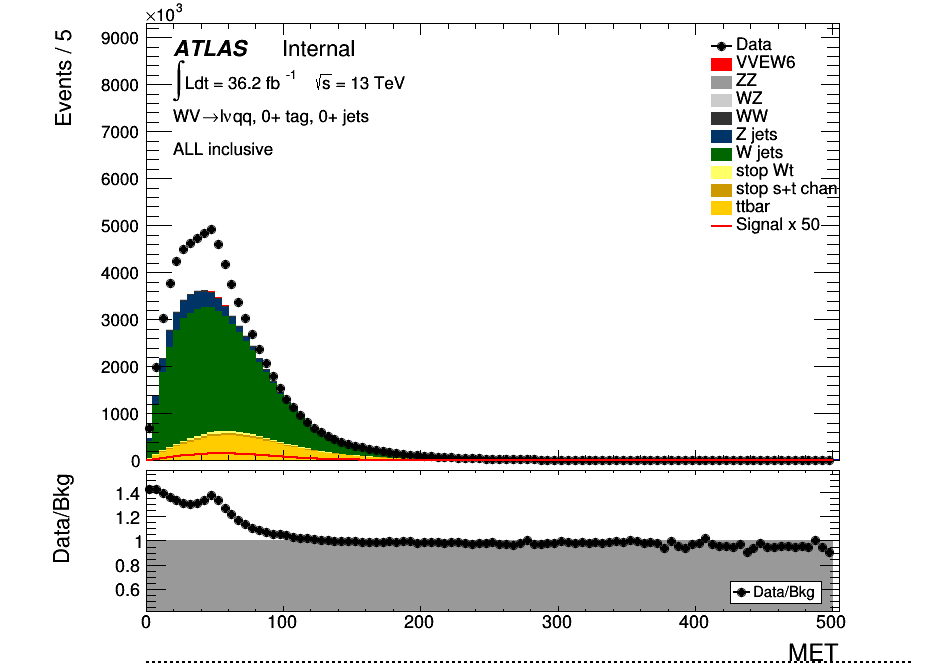
\includegraphics[width=\linewidth]{figures/1lep/CRPlots/C_0ptag0pjet_0ptv_ALL_MET_Lin.png}
            \caption{$E_{T,miss}$ before any event selection.}
        \end{subfigure}
        \begin{subfigure}{0.3\textwidth}
            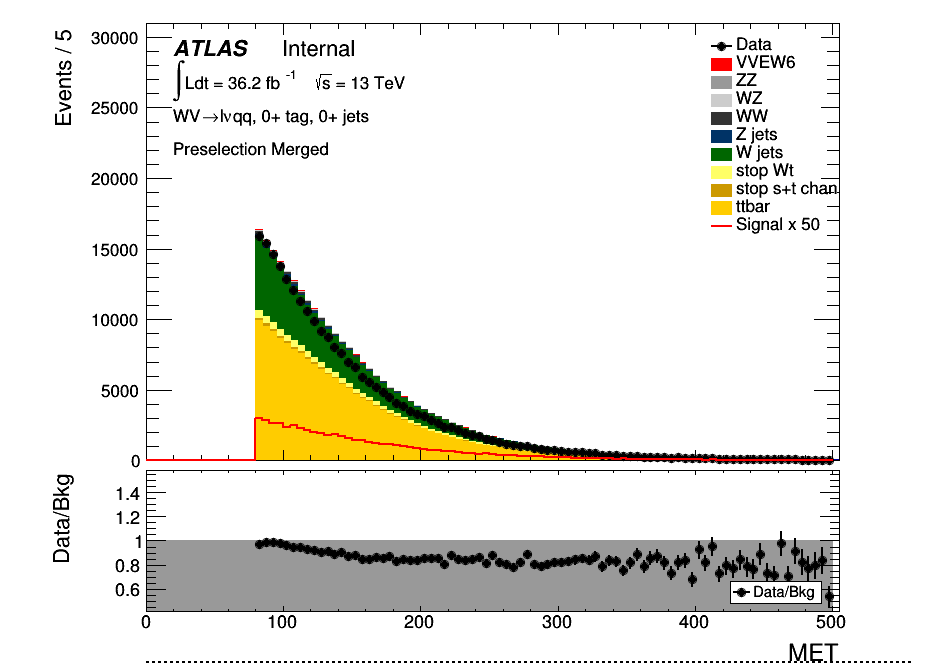
\includegraphics[width=\linewidth]{figures/1lep/CRPlots/C_0ptag0pjet_0ptv_Presel_Merged_MET_Lin.png}
            \caption{$E_{T,miss}$ after merged common preselection.}
        \end{subfigure}
        \begin{subfigure}{0.3\textwidth}
            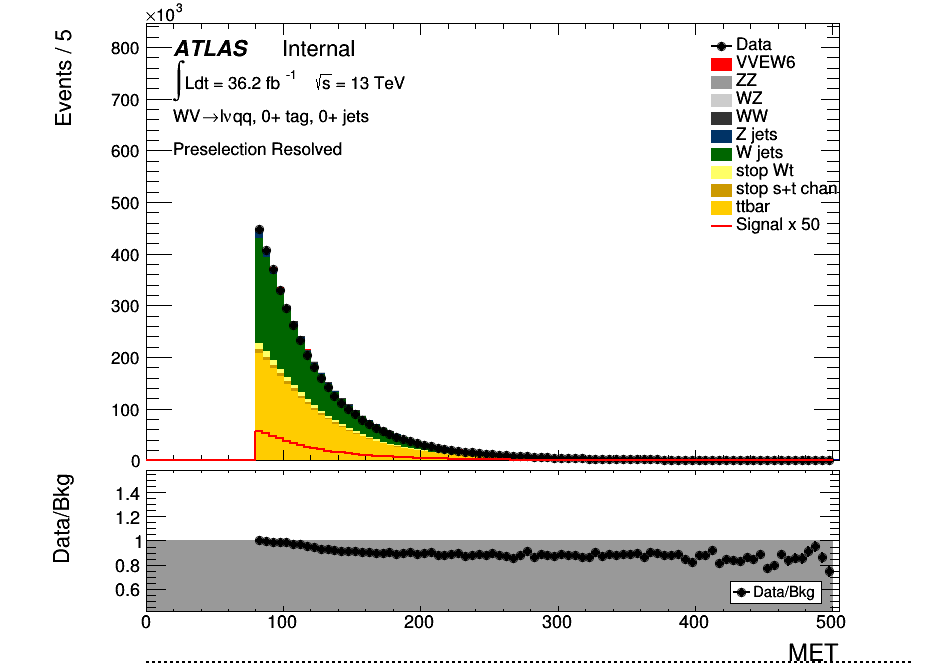
\includegraphics[width=\linewidth]{figures/1lep/CRPlots/C_0ptag0pjet_0ptv_Presel_Resolved_MET_Lin.png}
            \caption{$E_{T,miss}$ distribution after resolved common preselection.}
        \end{subfigure} \\

        \begin{subfigure}{0.3\textwidth}
            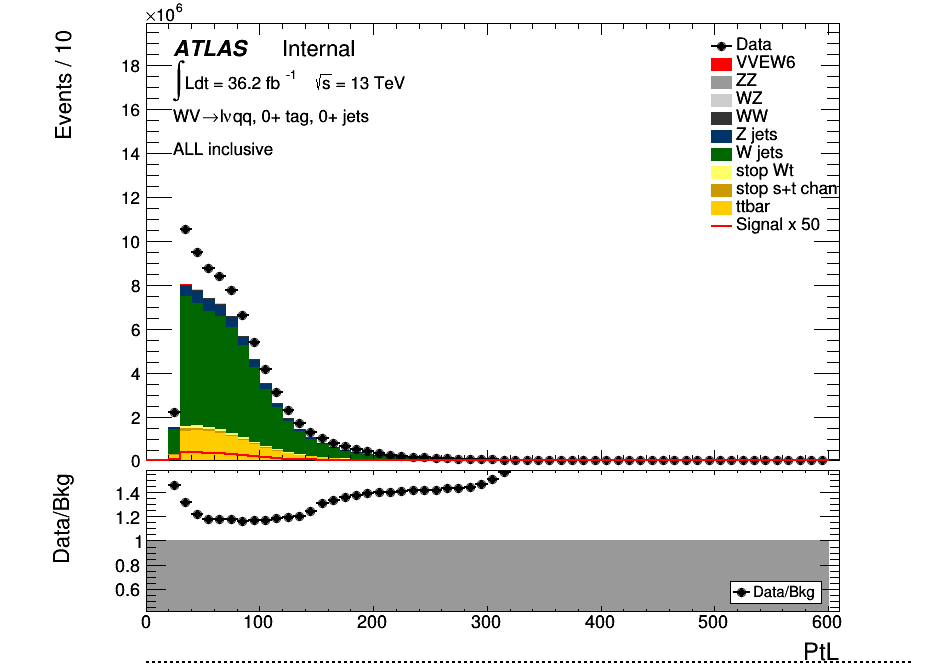
\includegraphics[width=\linewidth]{figures/1lep/CRPlots/C_0ptag0pjet_0ptv_ALL_PtL_Lin.png}
            \caption{$p_{T,l}$ before any event selection.}
        \end{subfigure}
        \begin{subfigure}{0.3\textwidth}
            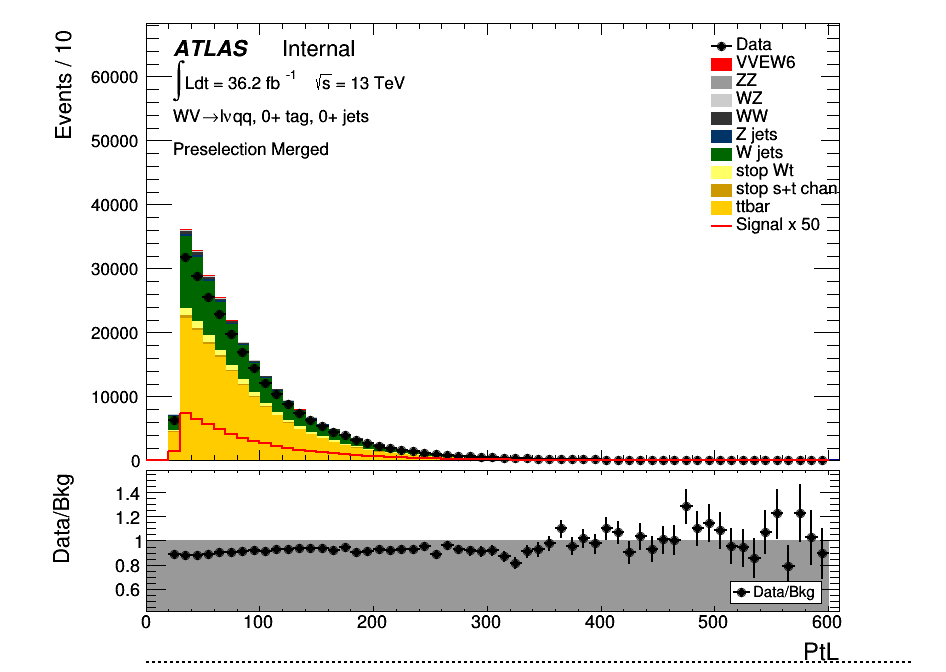
\includegraphics[width=\linewidth]{figures/1lep/CRPlots/C_0ptag0pjet_0ptv_Presel_Merged_PtL_Lin.png}
            \caption{$p_{T,l}$ after merged common preselection.}
        \end{subfigure}
        \begin{subfigure}{0.3\textwidth}
            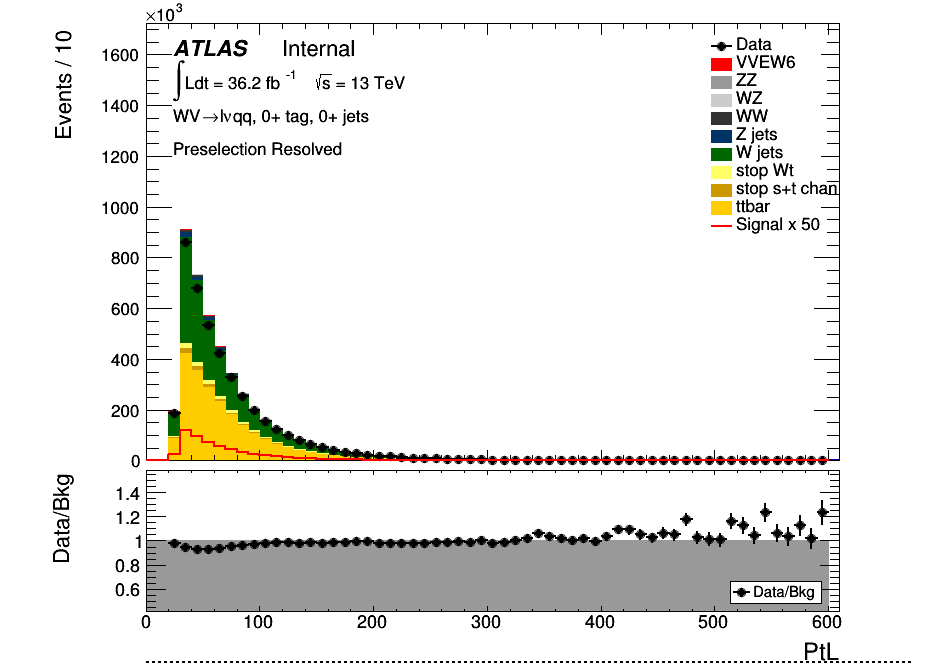
\includegraphics[width=\linewidth]{figures/1lep/CRPlots/C_0ptag0pjet_0ptv_Presel_Resolved_PtL_Lin.png}
            \caption{$p_{T,l}$ distribution after common resolved preselection.}
        \end{subfigure} \\

        \begin{subfigure}{0.3\textwidth}
            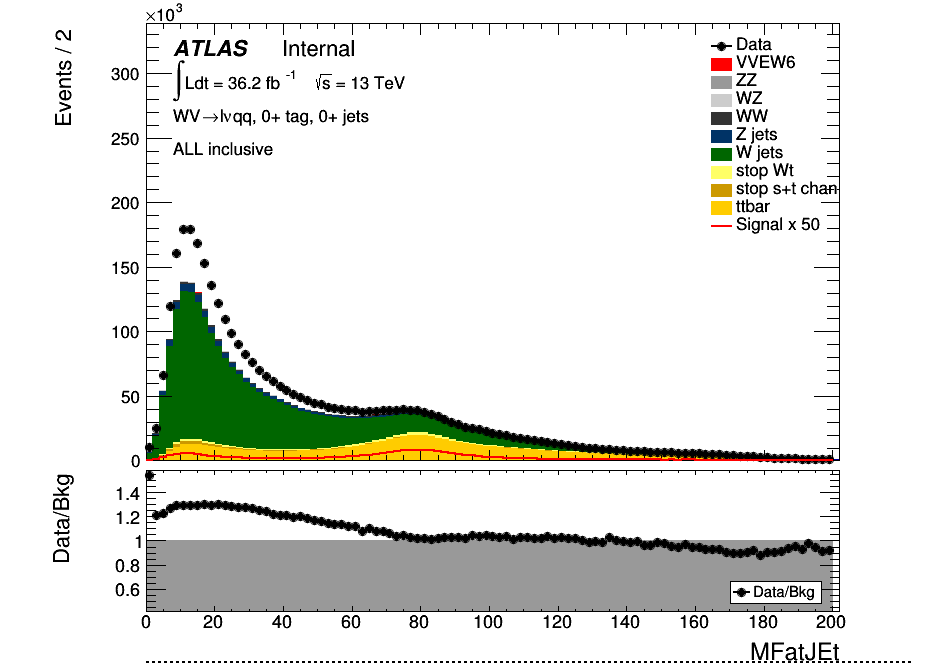
\includegraphics[width=\linewidth]{figures/1lep/CRPlots/C_0ptag0pjet_0ptv_ALL_MFatJet_Lin.png}
            \caption{$M_{J}$ before any event selection.}
        \end{subfigure}
        \begin{subfigure}{0.3\textwidth}
            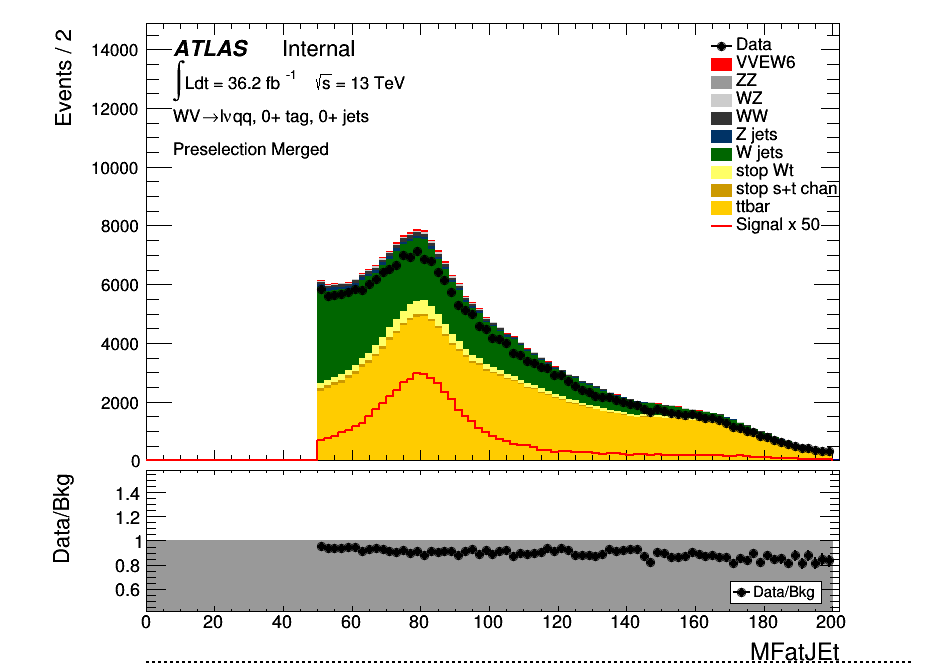
\includegraphics[width=\linewidth]{figures/1lep/CRPlots/C_0ptag0pjet_0ptv_Presel_Merged_MFatJet_Lin.png}
            \caption{$M_{J}$ after merged common preselection.}
        \end{subfigure}

        \caption{Distributions for $E_{T,miss}$, $E_{T,miss}$, and $m_{J}$ in the 1 lepton channel at different stages of the analysis selection; preselection merged and preslection resolved labels refers to the set of cuts applied in the merged and resolved regime rather than the boson tagger cuts (merged) and the signal jets mass window cut.}
        \label{fig:1LepPreselCuts}
\end{figure}


%%%\begin{figure}[ht]
%%%\centering
%%%	\subfigure[$E_{T,miss}$ before any event selection.]{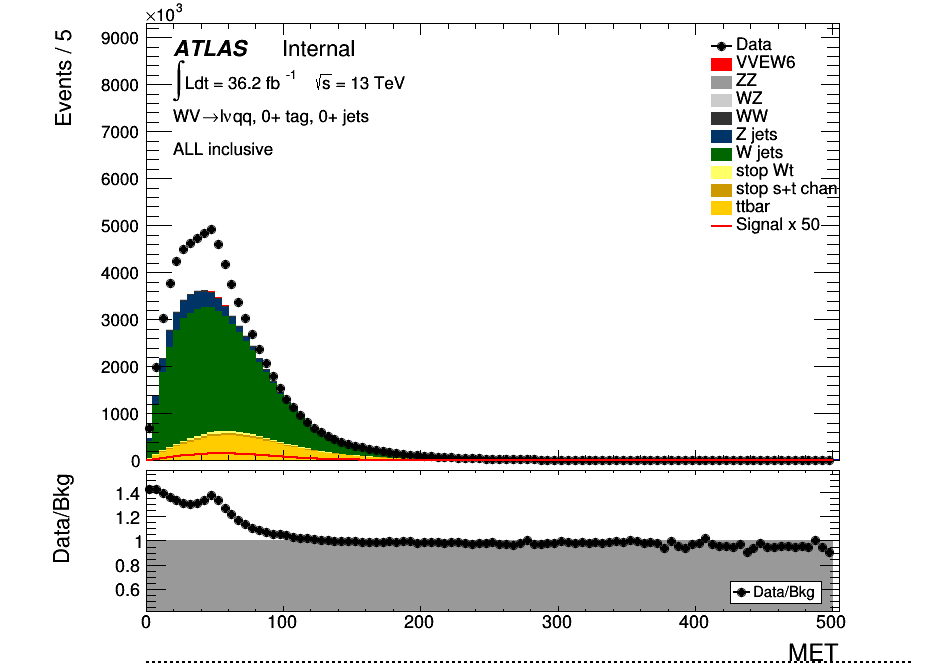
\includegraphics[width=0.3\textwidth]{figures/1lep/CRPlots/C_0ptag0pjet_0ptv_ALL_MET_Lin.png}} 
%%%	\subfigure[$E_{T,miss}$ after merged common preselection.]{\includegraphics[width=0.3\textwidth]{figures/1lep/CRPlots/C_0ptag0pjet_0ptv_Presel_Merged_MET_Lin.png}} 
%%%	\subfigure[$E_{T,miss}$ distribution after resolved common preselection.]{\includegraphics[width=0.3\textwidth]{figures/1lep/CRPlots/C_0ptag0pjet_0ptv_Presel_Resolved_MET_Lin.png}} \\
%%%
%%%	\subfigure[$p_{T,l}$ before any event selection.]{\includegraphics[width=0.3\textwidth]{figures/1lep/CRPlots/C_0ptag0pjet_0ptv_ALL_PtL_Lin.png}} 
%%%	\subfigure[$p_{T,l}$ after merged common preselection.]{\includegraphics[width=0.3\textwidth]{figures/1lep/CRPlots/C_0ptag0pjet_0ptv_Presel_Merged_PtL_Lin.png}} 
%%%	\subfigure[$p_{T,l}$ distribution after common resolved preselection.]{\includegraphics[width=0.3\textwidth]{figures/1lep/CRPlots/C_0ptag0pjet_0ptv_Presel_Resolved_PtL_Lin.png}} \\
%%%
%%%	\subfigure[$M_{J}$ before any event selection.]{\includegraphics[width=0.3\textwidth]{figures/1lep/CRPlots/C_0ptag0pjet_0ptv_ALL_MFatJet_Lin.png}} 
%%%	\subfigure[$M_{J}$ after merged common preselection.]{\includegraphics[width=0.3\textwidth]{figures/1lep/CRPlots/C_0ptag0pjet_0ptv_Presel_Merged_MFatJet_Lin.png}} 
%%%
%%%	\caption{Distributions for $E_{T,miss}$, $E_{T,miss}$, and $m_{J}$ in the 1 lepton channel at different stages of the analysis selection; preselection merged and preslection resolved labels refers to the set of cuts applied in the merged and resolved regime rather than the boson tagger cuts (merged) and the signal jets mass window cut.}
%%%	\label{fig:1LepPreselCuts}
%%%\end{figure}


%After the $W \to \ell\nu$ selection above and $W/Z \to jj$ selection described in Section~\ref{subsubsec:resolved_jets_selection},
%the following selection cuts are required to take the event topology of which two high-\pt\ bosons are back--to--back in the $x$--$y$ plane:
%\begin{itemize}
%\item $\Delta \phi(\ell, \met)< XX$;
%\item $\Delta \phi(j1,j2) < XX$;
%\item $\Delta \phi(\ell,j1(2)) > XX$;
%\item $\Delta \phi(j1(2), \met) > XX$;
%\end{itemize}
%where $\Delta \phi(i, j)$ is the distance in the  coordinate between objects $i$ and $j$.

%%% 2-leptons channel

%In particular, modelling of the leading and sub-leading muon \pt look slighlty different. 
%This is an effect of the first bin in both distributions that has different values in the 
%data/MC ratio. After removing the first bin in the subleading muon \pt distribution the modelling
%qfor the two muons \pt is consistent as checked in Appendix \ref{app:leptonin2lep}.


%
\clearpage
\subsection{VBS Selection}
\label{subsec:vbs_selection}

In all three channels events are required to contain a small-R jet pair as a candidate VBS jets, we refer to them as Tag Jets. 

The hadronically-decaying $W/Z$ candidate is reconstructed as either two small-$R$ jets~($j$)
or one large-$R$ jet~($J$), as explained in the following sections \ref{subsubsec:merged_jets_selection}-\ref{subsubsec:resolved_jets_selection}; therefore, each event should contain at least four small-$R$ jets in the resolved analysis or one large-$R$ jet and
two small-$R$ jets in the merged analysis. 

The strategy to select first tag jets and then signal jets which came from $W/Z$ from the remaining jets is chosen; 
this is motivated from the preference to focus on the production topology first (VBS jets) 
and then move to identify the objects related to the decay part of the target process. 
%Furthermore, this choice is consistent what the strategy performed in the VV semi-leptonic resonant search \cite{Bachas:2646593}.

The tagging jets algorithm is quite usual to what is done in analyses in ATLAS.

Tagging jets are required, 
firstly, 
%to be non-$b$-tagged; this would help in order to suppress the contribution of diagrams with a $Wtb$ vertex
%(especially the electroweak $t\bar{t}$ production) in the electroweak $VVjj$ production. 
%Furthermore, 
%fJVT selection has been applied to the small-R jets; 
to pass the fJVT selection, the Loose fJVT WP is used.
%the jets are required to pass the Loose fJVT WP as additional criteria to be selected as tagging jets. 
The Loose WP has been chosen for simplicity, indeed, it is the default WP recommended 
and the related SF are by default available in our analysis framework; 
furthermore, no significant difference with respect to the Tight WP has been observed, 
more details are given in dedicated studies reported in appendix \ref{app:fjvt}.
Furthermore, b-veto has been investigated to be applied on all the jets of the collection
before pairing the candidates, since, no significant impacts has been found,
as documented in the Appendix \ref{app:tagjet_bveto}, no b-jet requirement is applied on the taggging jets.

The tagging jets candidates must be in the opposite hemispheres, 
$\eta_{\mathrm{tag}\ j_1} \cdot \eta_{\mathrm{tag}\ j_2} < 0$,
and to have the highest dijet invariant mass among all the possible pairs of small-R jets in the event, 
that have passed already 
%b-tagging veto and 
the fJVT requirement, as mentioned above.
 
After the tagging jet pair are selected, it is required that both tagging jets should have \pT$>$30~\GeV and that the invariant mass of the two tagging jets system is greater than 400~\GeV; 
%we rely on the optimisation studies done in the previous round of the analysis on the choice of both \pT and invariant mass cuts. 
As an example, the \mjjtag distribution for both data and MC samples is shown before the cut in the \zlep channel SRs Figure \ref{fig:0lepMjj}; 
the \mjjtag re-weighting is already applied and it will be described in section \ref{subsec:mjj_reweight}.

\begin{figure}[ht]
    \centering
    \subfigure[merged HighPurity]{\includegraphics[width=0.3\textwidth]{figures/0lep/cutflow/nominal/merged/plots/soverb_individual_SRVBS_HP_MTagMerJets400_MTagMerJets_cutflow.pdf}}
    \subfigure[merged LowPurity]{\includegraphics[width=0.3\textwidth]{figures/0lep/cutflow/nominal/merged/plots/soverb_individual_SRVBS_LP_MTagMerJets400_MTagMerJets_cutflow.pdf}}
    \subfigure[resolved]{\includegraphics[width=0.3\textwidth]{figures/0lep/cutflow/nominal/merged/plots/soverb_individual_SRVBS_Res_MTagResJets400_MTagResJets_cutflow.pdf}}
    \caption{0-lepton $m(jj)^\text{tag}$ selection. The distributions are shown for the three SR selections; the specific definition of each of them (HighPurity, LowPurity, Resolved) will be given in the following Section \ref{subsec:sr_selection}. Entering are events passing the respective selection up to the point of the $m(jj)^\text{tag}$ cut which is shown by the vertical line.} 
    \label{fig:0lepMjj}
\end{figure}




%
%%\clearpage
%%\subsection{Signal Regions (SRs) definitions}
\label{subsec:sr_selection}

Multiple Signal Regions (SRs) are defined to optimize the signal sensitivity and to accommodate the different reconstruction regimes of the hadronically decaying boson ($V \rightarrow qq$). The Merged regime is prioritized over the Resolved regime. Detailed descriptions of these two regimes are provided in this section.

%\subsection{Selection of $W/Z \to J$ candidates (merged category)}
\subsection{Selection of \texorpdfstring{$W/Z \to J$}{W/Z -> J} candidates (merged category)}
\label{subsubsec:merged_jets_selection}

For boosted (high-energy) boson production, where the \pt of hadronically decaying $W/Z$ bosons is at least 200 GeV, each boson is frequently reconstructed as a single large-$R$ jet. In this ``merged'' category, the selection requires at least one large-$R$ jet, with the leading large-$R$ jet utilized for $W/Z$ candidate reconstruction. To avoid double-counting jet energy, the large-$R$ jet must be separated by a distance greater than $|\Delta R| = 1.4$ from both VBS Tag Jets.
%
The final step in selecting boosted $W/Z \to qq$ candidates involves boson tagging based on three variables: jet mass ($m_{J}$), substructure variable $D_2$, and ungroomed track multiplicity ($n_{\text{Tracks}}$).
We adopt tagger working points (WPs) recommended for $50\%$ and $80\%$ signal efficiencies, applied at the jet level to optimize the selection.

To establish orthogonal regions, we define:
\begin{itemize}
    \item High-Purity (HP) Region: Includes events (and their corresponding single large-R jet) that meet the $50\%$ WP criteria.
    \item Low-Purity (LP) Region: Includes events that satisfy the $80\%$ WP but do not fulfill the $50\%$ WP criteria.
\end{itemize}
Thus, events in the merged regime conforming to the $50\%$ WP criteria are categorized into the HP Signal Region (SR), while those meeting the $80\%$ WP standards but not the $50\%$ are allocated to the LP SR. Table~\ref{tab:1lep_merged} contains the complete definitions of the HP and LP SRs.

For the HP SR, the $50\%$ WP $W/Z$-tagging scale factor is applied. For the LP SR, a custom scale factor is defined:

    \begin{equation}
    SF_{LP} = \frac{\epsilon_{loose}SF_{eff,loose}- \epsilon_{tight}SF_{eff,tight} }{ \epsilon_{loose}- \epsilon_{tight}}
    \end{equation}
Here, $\epsilon$ represents the efficiency estimated in \ttbar events for signal and $\gamma$+jets and multijet events for background.
``Loose'' corresponds to the $80\%$ WP, while ``tight'' refers to the $50\%$ WP. Detailed discussions on $W/Z$-tagging scale factors are available in Section \ref{subsec:bkg_uncer_vtagger}.

In the baseline boson tagger, exclusive selections for $Z$ and $W$ candidates are used. However, due to significant overlap in these selections, it is not feasible to define two orthogonal regions for the hadronic decays of $W$ and $Z$. Therefore, an inclusive $V \to qq$ selection is utilized, which is a logical OR of the $W$ and $Z$ boson tagger selections. This inclusive selection adopts the lower mass cut from the $W$ selection and the upper cut from the $Z$ selection.


\subsection{Selection of $W/Z \to jj$ candidates (resolved category)}
\label{subsubsec:resolved_jets_selection}

In the lower \pt range for hadronically decaying $W/Z$ bosons, two distinct jets are typically resolvable. This resolved regime offers the highest efficiency for EW $VV+jj$ signals, although its sensitivity is marginally lower compared to the merged regime due to increased background acceptance.
Within this regime, events are selected based on the presence of at least two ``signal'' jets. These signal jets are identified from a pool of candidates, excluding the two VBS Tag Jets.

In the search of $W/Z$ candidates, we select the two signal jets with the highest \pt. This approach slightly reduces signal efficiency within the mass window compared to previous analyses. However, it allows for a more relaxed application of the Close-$V$ selection algorithm, which pairs jets with invariant masses closest to the nominal $V$($W/Z$) boson masses. 

After selecting the two jets of interest, the leading jet is required to have \pt $\SI{>40}{\GeV}$, a criterion set to further reduce background and enhance sensitivity. To identify events indicative of a hadronically decaying $W/Z$ boson, the dijet mass ($m_{jj}$) is constrained within a mass window of $64 <m_{jj}<106\,\GeV$.

Figure~\ref{fig:1lepMVHadResSR} shows the full range distributions for $m_{jj}$ without the mass window constraints, with the $W$ peak coming from top-associated processes clearly visible.

As mentioned in Section~\ref{sec:mc_sample_ewvvjj}, a VBS-enhancing cut, $m_{jjj} > 220\,\si{\GeV}$, is introduced later in the analysis to reduce the contribution from the non-VBS $tZb$ process, as illustrated in Fig.~\ref{fig:feynmantZb}. This cut, implemented near the reconstructed top mass, is shown in Figure~\ref{fig:1lepWCR_mjjj} in the next section. Events passing this cut are classified into ``tight'' regions, while those that do not are classified into ``loose'' regions. The resolved ``tight'' regions are used in calculations and statistical studies, whereas the resolved ``loose'' regions serve as a sanity check.

\begin{figure}[ht]
    \centering
    \begin{subfigure}{0.32\textwidth}
        \includegraphics[width=\linewidth]{figures/event_selection/ALL_MVHadRes.pdf}
        \caption{Before any event selection.}
    \end{subfigure}
    \begin{subfigure}{0.32\textwidth}
        \includegraphics[width=\linewidth]{figures/event_selection/Presel_Resolved_MVHadRes.pdf}
        \caption{After resolved preselection.}
    \end{subfigure}
    \caption{Reconstructed mass distribution of the leading two jets.}
    \label{fig:1lepMVHadResSR}
\end{figure}

\subsection{VV system invariant mass}
\label{subsubsec:mVV_reconstruction}

The mass of the $WV$ system, $m_{WV}$, is calculated using the lepton, neutrino, and the hadronically-decaying boson (represented by either a large-$R$ jet or two small-$R$ jets). To determine the neutrino's momentum in the $z$-direction ($p_z$), we apply the Particle Data Group (PDG) value for the $W$ boson mass to the lepton-neutrino system. This results in a quadratic equation. The solution for $p_z$ is chosen based on the following criteria: if the solutions are complex, the real component is taken; if they are real, the solution with the smaller absolute value is selected.

%%%%%

%
%\subsection{EW Top production veto}
\subsubsection{EW Top production veto: Tight region definition}
\label{subsec:topveto_selection}

We found that the contribution of the EW Top production is still significant in our SRs. 

As discussed in Section~\ref{sec:mc_sample_ewvvjj},
the EW Top and VVV processes are included in the signal MC samples. Since we want to enhance the VBS processes in our target phase space for the interpretation of data/MC agreement with the aQGC new physics model, we add additional selections to reduce the top contribution.

%\textcolor{red}{put here a table of the VV, VVV and top contributions in the SRs}

%\subsubsection{Loose and tight regions definition}
\label{subsec:LooseTightRegion}

We found that the resolved regions have much higher top contribution with respect to the merged ones.
For the top contribution in our signal sample, the top-quark mass can be reconstructed in the resolved SRs.
Two signal jets and the additional third jet which forms the three-jet mass, $m_{jjj}$, 
the closest to the top mass (172.76 \ GeV) are used. 
Additional third jet was chosen from all jets except for signal jets, including VBS tagging jets.
Figure \ref{fig:2leptopMass}-a shows the $m_{jjj}$ distributions for top contribution, VVV, and other components (e.g. VBS) in the EW WZjj signal sample.
We can reject the top contribution by the cut on $M_{jjj}$ at 220~\GeV.
Figure \ref{fig:2leptopMass}-b shows the data/MC comparison of the $M_{jjj}$ distribution in the \tlep \Zjets CR.
The mis-modelling in Z+jets shown in $m_{tagjj}$ was also seen in $M_{jjj}$ distribution. It is also corrected by re-weighting with $m_{tagjj}$ described in section~\ref{subsec:mjj_reweight}, though a slight slope is seen in figure \ref{fig:2leptopMass}-b, which seems to be re-weighted a little too much in this phase space.

\begin{figure}[ht]
    \begin{center}
    	\subfigure[$\text{top mass peak}$]{\includegraphics[width=0.4\textwidth]{figures/2lep/topMass/WZjjtopMasspeak.png}}
    	\subfigure[$\text{top mass in CRVjet}$]{\includegraphics[width=0.4\textwidth]{figures/2lep/dataMC/C_0ptag2pjet_0ptv_CRVjet_topMass_Log.png}}
        \caption{ Mass of 3 jets in the 2-lepton channel; shapes of the signal components in the Resolved SR (a) and data to MC comparison in the \Zjets CR (b) are shown.} 
        \label{fig:2leptopMass}
    \end{center}
\end{figure}

Figure \ref{fig:0leptopMass} shows distributions for the reconstructed top mass in the \zlep channel; 
in particular, only data, signal and top background are shown to stress the most of the top background 
is rejected by this cut, while the actual data, containing the other SM background as well as the EWK signal
have higher selection efficiency in the high reconstructed top mass. 
Furthermore, the bottom pannel shows the signal to background ration that in increasing with this variable.

\begin{figure}[ht]
    \begin{center}
    	\subfigure[merged HP SR]{\includegraphics[width=0.45\textwidth]{figures/0lep/cutflow/topcheck/merged/plots/soverb_individual_SRVBS_HP_cutTopMassMer_topMassMer_cutflow.pdf}}
    	\subfigure[resolved SR]{\includegraphics[width=0.45\textwidth]{figures/0lep/cutflow/topcheck/merged/plots/soverb_individual_SRVBS_Res_cutTopMassRes_topMassRes_cutflow.pdf}}
        \caption{ Mass of $J^\text{sig}j^\text{extra}$ in merged (left) and of 3 jets $(jj)^\text{sig}j^\text{extra}$ in resolved in the \zlep channel signal regions. In particular, only the top background is shown, actual data contains also the other SM background, therefore, the data/MC is not expected to overlaid in the top pannel.} 
        \label{fig:0leptopMass}
    \end{center}
\end{figure}

The resolved SRs are divided into two sub-categories:
\begin{itemize}
  \item Loose Resolved: this is the baseline region defined in Section~\ref{subsubsec:resolved_jets_selection}, and
  \item Tight Resolved: Loose Resolved + $M_{jjj} > 220 GeV$.
\end{itemize}

\subsubsection{Signal purity in merged and resolved regimes}
\label{subsec:SignalPurity}

The contribution of the three truth components of the EW signal has been checked with previous SR definition and with new $M_{jjj}$ selections. 

Tables
\ref{tab:0leptopMassTable}-
\ref{tab:TruthTop1LepPurity}-
\ref{tab:TruthTop2LepPurity}
%shows the summary for the \olep channel; 
show the summary of purity picture applying the tight cut for the resolved and merged regimes 
respectively, in the \zlep-\olep-\tlep channels.

Based on the improvements and studies performed, the reconstructed top-mass cut is only applied in the resolved signal region to define the new tight signal region, and the merged signal regions are left as they are.

\begin{table}[ht]
    \centering
    \begin{tabular}{r|c|c|c|c}
         & \multicolumn{2}{c|}{merged HP SR} & \multicolumn{2}{c}{resolved SR}\\
         & before cut & after cut & before cut & after cut\\
         \hline
         truth top fraction in signal MC & $17\%$ & $13\%$ &$33\%$ & $9\%$ \\
         signal MC events & $94$ & $77$ & $594$ & $219$ \\
         top ($t\bar t$ + single $t$) MC events & $1786$ & $819$ & $18208$ & $1642$ \\
        \end{tabular}
        \caption{Effect of 3 jet cut in 0-lepton merged HP and resolved SR.} 
        \label{tab:0leptopMassTable}
\end{table}

\begin{table}[ht]
    \centering
	\resizebox{0.7\textwidth}{!}{
	\begin{tabular}{|c||c|c||c |c|}
    \hline
        & \shortstack{ VBS enhanced \\(resolved)} & \shortstack{non VBS enhanced \\ (resolved)} & \shortstack{VBS enhanced \\ (merged)} & \shortstack{non VBS enhanced \\ (merged)}\\
    \hline
    Truth Top       & 56.3 & 135.7 & 6.42 & 8.05 \\ 
    \hline
    Truth Triboson  & 3.85 & 9.08 & 1.72 &  2.178\\
    \hline
    Truth VBS       &  148 & 224.9 & 43.8 & 47.58\\
    \hline
    VBS purity & .711 & .608 & .843 & .823 \\
    \hline
	\end{tabular}}
    \caption{Event yields for 1lepton EW6 events in the resolved signal region and high purity merged signal region. The resolved VBS enhanced signal region is defined as events that pass the loose resolved signal region and pass $M_{jjj} >$ 220GeV. The merged VBS enhanced region is defined as events that pass the usual merged high purity signal region and pass $M_{Jj} >$ 220Gev, where $M_{Jj}$ is defined similarly to $M_{jjj}$, as the mass of the large-R jet and a third jet with total mass closest to the top mass. non-VBS enhanced regions are the old loose signal region definitions. 
%Based on the improvements shown here, the $M_{jjj}$ cut is only applied in the resolved signal region to define the new tight signal region, and the merged signal regions are left as they are. 
    }
\label{tab:TruthTop1LepPurity}
\end{table}

\begin{table}[ht]
    \centering
	\resizebox{0.70\textwidth}{!}{
	\begin{tabular}{|c||c|c|c|c|}      
        \hline
                    & SRVBS (resolved) & VBS enhanced (resolved) & SRVBS (merged) & VBS enhanced (merged) \\ \hline
    Truth Top       & 0.48             & 0.14                    & 0.14           & 0.10                  \\ \hline
    Truth VVV       & 0.03             & 0.03                    & 0.08           & 0.08                  \\ \hline
    Truth VBS       & 0.49             & 0.83                    & 0.78           & 0.82                  \\ \hline
	\end{tabular}
    }
    \caption{Fraction of event yields for 2lepton channel. Only EWWZjj events are checked here since there are no Top contributions in EWZZjj events.}
    \label{tab:TruthTop2LepPurity}
\end{table}

%\textcolor{red}{we put here the purities of the MC signal samples in the final reco regions comparing the diagram based classification for VV, VVV and EWTop}

%
\clearpage
\subsection{Control Regions (CRs) definitions}
\label{subsec:cr_selection}

We use a combined MC template and data-driven background estimation, indeed, we rely on the MC simulations samples for the SM background processes, but we use dedicated Control Regions (CRs) to constrain the normalization of the background expectation in the SRs.

The dedicated CRs to the $Z$+jets, $W$+jets and \ttbar events are defined in this section.

The $Z$+jets, $W$+jets and \ttbar CRs are used in this analysis shared 
across the the 0-, 1- and 2-lepton channels;
for instance, the \ttbar CR is defined using \olep events only, 
and used to constraint this background in all the SRs.
Independent CRs for resolved and merged categories are, instead,
used to account for possible mis-modelling of the background depending on \pt range.

\subsubsection{$W$+jets CR (WCR) and $Z$+jets CR (ZCR)}
%\textbf{$W$+jets CR (WCR) and $Z$+jets CR (ZCR)}

The $V$+jets CR (VCR) for $V=W/Z$, $W$+jets CR (WCR), and $Z$+jets CR (ZCR) are defined using the mass sidebands with respect to hadronically decaying vector boson in 0-, 1-, and 2-lepton channels, respectively.
The event selections are otherwise the same as the SR selections.
For the simplicity of the analysis, the common sideband is defined as the outside of both $W\to q\bar{q}$ and $Z \to q\bar{q}$ signal regions.
The same definition is used in all channels:
In the resolved category, a requirement of $50 < m_{jj} < 64$ GeV or $m_{jj} > 106$ GeV is applied which is an inversion of the $m_{jj}$ cut in the corresponding SR.
In the merged case, the event has to fail the vector boson tagger's lower working point of $\epsilon=80\%$.
%In the merged category, the purity of the $W$+jets background is 77\,\% in the lower mass side band, 62\,\% in the higher mass side band region and 65\,\% in total. The $t\bar{t}$ contamination is 30\,\% in higher mass side band regions. 

Figure \ref{fig:1lep2lepMVHadResCR} shows an example of sideband distributions in the resolved regions.
Figure \ref{fig:1lep2lepMVHadMerCR} shows an example of fat jet mass distributions in the merged control region; 
since the merged CR is defined using the full tagger 80\% WP, the mass distribution collects events both 
in the sidebands both in the mass window.

\begin{figure}[ht]
    \centering
    \begin{subfigure}{0.3\textwidth}
        \includegraphics[width=\linewidth]{figures/1lep/CRPlots/C_0ptag2pjet_0ptv_CRVjet_MVHadRes_Lin.png}
        \caption{\emph{\olep, resolved WCR}}
    \end{subfigure}
    % You can add other subcaptions here if needed
    \caption{$m_{jj}$ plot in the sidebands in \zlep channel VCR (a), in \olep WCR (b) and \tlep channel ZCR (right).}
    \label{fig:1lep2lepMVHadResCR}
\end{figure}

%\begin{figure}[ht]
%    \begin{center}
%        \subfigure[]{\includegraphics[width=0.3\textwidth]{figures/1lep/CRPlots/C_0ptag2pjet_0ptv_CRVjet_MVHadRes_Lin.png}}
%        \caption{ $m_{jj}$ plot in the sidebands in 1-lepton channel. }
%    \end{center}
%    \label{fig:1lepMVHadResCRVjet}
%\end{figure}

\subsubsection{$t\bar{t}$ CR (TCR)}
%\textbf{$t\bar{t}$ CR (TCR)}

%Two sets of the \ttbar CR (TR1 and TR2) can be used in this analysis.

In 1-lepton channel, TCR is defined by requiring at least one $b$-tagged jet instead of $b$-veto; distributions of the b-jets multiplicity for both resolved and merged regime are shown in figure \ref{fig:1lepNBjetsPresel}. 
%The purity of the $t\bar{t}$ background in this 
%region is 85\,\%. Signal contamination in both $W$+jets and $t\bar{t}$ control regions is negligible. The purity 
%of $W$+jets in WR is a bit poor, but the simultaneous fit to TR and WR makes it possible to determine the 
%normalization of $W$+jets correctly, thanks to high purity of $t\bar{t}$ in TR.

Since, the orthogonal cut is represented by the additional bjets in the event, 
the TCR correspond to mass window phase spaces, therefore, for the merged regime
TCR inherit the HP and LP splitting as for the SRs.

\begin{figure}[ht]
    \centering
    \begin{subfigure}{0.3\textwidth}
        \includegraphics[width=\linewidth]{figures/1lep/CRPlots/C_0ptag0pjet_0ptv_Presel_Merged_NBJets_Lin.png}
        \caption{After merged preselection}
    \end{subfigure}
    \begin{subfigure}{0.3\textwidth}
        \includegraphics[width=\linewidth]{figures/1lep/CRPlots/C_0ptag0pjet_0ptv_Presel_Resolved_NBJets_Lin.png}
        \caption{After resolved preselection}
    \end{subfigure}
    \caption{Bjets multiplicity in the 1-lepton channel, after common preselection cuts have been applied.}
    \label{fig:1lepNBjetsPresel}
\end{figure}



%
\clearpage
\subsubsection{Signal and background cut-flows}
\label{subsec:cutflows}

Cutflow Tables are presented for different signal regions.

\zlep: Figure~\ref{tab:0lepCutFlow}.
\olep: Figure~\ref{fig:1lepCutFlow}.
\tlep: 
Tables~\ref{tab:2lep_HPSR},
\ref{tab:2lep_LPSR},
\ref{tab:2lep_ResolvedSR},
\ref{tab:2lep_MergedCR}, and
\ref{tab:2lep_ResolvedCR}.

Tables
\ref{tab:PrefitYield_TCRHP_Per}-
\ref{tab:PrefitYield_TCRLP_Per}-
\ref{tab:PrefitYield_TCRRes_Per} (TCR)-
\ref{tab:PrefitYield_VCRMer_Per}-
\ref{tab:PrefitYield_WCRMer_Per}-
\ref{tab:PrefitYield_ZCRMer_Per}-
\ref{tab:PrefitYield_VCRRes_Per}-
\ref{tab:PrefitYield_WCRRes_Per}-
\ref{tab:PrefitYield_ZCRRes_Per} (VCR)-
\ref{tab:PrefitYield_0lepHPSR_Per}-
\ref{tab:PrefitYield_1lepHPSR_Per}-
\ref{tab:PrefitYield_2lepHPSR_Per} (HPSR)-
\ref{tab:PrefitYield_0lepLPSR_Per}-
\ref{tab:PrefitYield_1lepLPSR_Per}-
\ref{tab:PrefitYield_2lepLPSR_Per} (LPSR)-
\ref{tab:PrefitYield_0lepResSR_Per}-
\ref{tab:PrefitYield_1lepResSR_Per}-
\ref{tab:PrefitYield_2lepResSR_Per} (ResolvedSR)
show the final yields, in percentages, of the different CRs and SRs; 
the uncertainties account for statistical and systematic sources.


%%% 2-leptons channel
%%% HPSR 
\begin{table}[ht!]
\small
\caption{Cutflow table for HPSR region in \tlep channel. PassCommon cut refers to the lepton pre-selection and SFLetpons to the requirement to have SameFlavor leptons.}
\label{tab:2lep_HPSR}
\begin{center}
\resizebox{\textwidth}{!}{

 \begin{tabular}{ r ||  r  r  r  r  r  r  r  r  r  || r r r r r |}
 \ensuremath{\sqrt{s}=13 TeV}, \ensuremath{\mathcal{L}=139 fb^{-1}}  & W & WZ & WW & Z & ZZ & stopWtDilep & stops & stopt & ttbar & S & B & S/B & \ensuremath{S/\sqrt{B}}\tabularnewline
 \hline
All & 768630 & 118757 & 7549.85 & 2.69014e+07 & 75904.3 & 219335 & 1566.79 & 30086.3 & 3.4463e+06 & 8530.6 &3.15695e+07&0.000270216 & 1.51826\tabularnewline \hline
passCommon & 8949.67 & 73105.4 & 138.511 & 1.59613e+07 & 48170 & 22208.8 & 61.7359 & 1002.7 & 361153 & 3577.38&1.64761e+07&0.000217125 & 0.881328\tabularnewline \hline
TwoTagMerJets & 5430.67 & 41182 & 83.2249 & 9.38413e+06 & 24924.9 & 14016.8 & 33.1233 & 711.353 & 243694 & 2890.74&9.7142e+06&0.000297579 & 0.927483\tabularnewline \hline
PtTagMerJet1 & 4846.86 & 39715 & 80.198 & 7.66047e+06 & 23830.9 & 13522.8 & 31.7876 & 687.684 & 240045 & 2881.49 &7.98323e+06&0.000360943 & 1.01983\tabularnewline \hline
PtTagMerJet2 & 2692.05 & 26366.4 & 51.0517 & 3.74324e+06 & 14613 & 8652.04 & 19.427 & 455.492 & 180641 & 2527.77 &3.97673e+06&0.000635639 & 1.26758\tabularnewline \hline
AtLeastOneFatJet & 73.9896 & 1355.28 & 2.49747 & 54043.4 & 401.963 & 194.503 & 0.683082 & 9.52178 & 4071.51 & 190.792 &60153.4&0.00317176 & 0.777912\tabularnewline \hline
PtFatJet200 & 73.9896 & 1355.28 & 2.49747 & 54043.4 & 401.963 & 194.503 & 0.683082 & 9.52178 & 4071.51 & 190.792 &60153.4&0.00317176 & 0.777912\tabularnewline \hline
EtaFatJet2p0 & 73.9896 & 1355.28 & 2.49747 & 54043.4 & 401.963 & 194.503 & 0.683082 & 9.52178 & 4071.51 & 190.792 &60153.4&0.00317176 & 0.777912\tabularnewline \hline
dRL-eptonFatjet & 65.6967 & 1241.31 & 2.08247 & 50386.7 & 372.277 & 176.007 & 0.617677 & 8.85472 & 3270.23 & 177.47 &55523.8&0.0031963 & 0.753158\tabularnewline \hline
MFatJetLow & 26.3573 & 593.162 & 1.36814 & 17874.7 & 176.377 & 57.5099 & 0.147335 & 3.37462 & 1340.61 & 120.588 &20073.6&0.00600731 & 0.851124\tabularnewline \hline
SFLeptons & 8.29704 & 592.425 & 0.528064 & 17868.5 & 176.306 & 19.6953 & 0.0648612 & 1.36886 & 425.456 & 120.184 &19092.6&0.00629476 & 0.869786\tabularnewline \hline
MFatJet50 & 3.97632 & 321.546 & 0.150938 & 8269.29 & 98.0685 & 9.3015 & 0.0648612 & 0.426969 & 201.394 & 77.5594 &8904.22&0.00871041 & 0.821933\tabularnewline \hline
D2FatJet50 & 1.6553 & 164.963 & 0.150938 & 3032.68 & 52.9234 & 5.01844 & 0.0207499 & 0.246388 & 81.719 & 50.0044 & 3339.37&0.0149742 & 0.865317\tabularnewline \hline
NTrkFatJet50 & 1.24764 & 114.689 & 0.150938 & 1527.16 & 36.5107 & 2.48592 & 0.0207499 & 0.213116 & 41.1061 & 40.9103 &1723.59&0.0237356 & 0.985409\tabularnewline \hline
WZFatJet50 & 0.655411 & 112.269 & 0.150938 & 1469.7 & 35.6488 & 2.48592 & 0.0207499 & 0.213116 & 39.669 & 40.1491 &1660.82&0.0241743 & 0.985179\tabularnewline \hline
MTagMerJets400 & 0.608311 & 89.745 & 0.150938 & 1247.25 & 27.2269 & 2.34095 & 0.0207499 & 0.0789171 & 33.3017 & 37.6674 &1400.73&0.0268913 & 1.00644\tabularnewline \hline
\end{tabular}

}
\end{center}
\end{table}
%%
%%% LPSR 
\begin{table}[ht!]
\small
\caption{Cutflow table for LPSR region in \tlep channel}
\label{tab:2lep_LPSR}
\begin{center}
\resizebox{\textwidth}{!}{

 \begin{tabular}{ r ||  r  r  r  r  r  r  r  r  r  || r r r r r |}
 \ensuremath{\sqrt{s}=13 TeV}, \ensuremath{\mathcal{L}=139 fb^{-1}}  & W & WZ & WW & Z & ZZ & stopWtDilep & stops & stopt & ttbar &  S & B & S/B & \ensuremath{S/\sqrt{B}}\tabularnewline
 \hline
All & 768630 & 118757 & 7549.85 & 2.69014e+07 & 75904.3 & 219335 & 1566.79 & 30086.3 & 3.4463e+06 & 8530.6&3.15695e+07&0.000270216 & 1.51826\tabularnewline \hline
FailMergedSR50 & 768630 & 118667 & 7549.7 & 2.69001e+07 & 75877.1 & 219333 & 1566.77 & 30086.3 & 3.44627e+06 & 8492.93&3.15681e+07&0.000269035 & 1.51159\tabularnewline \hline
Trigger & 562963 & 108010 & 5681.35 & 2.40927e+07 & 69318 & 195862 & 1133.62 & 21873.2 & 3.02893e+06 & 7222.22 &2.80865e+07&0.000257142 & 1.36277\tabularnewline \hline
BothLepPt & 67751.3 & 90649.8 & 1147.71 & 2.07619e+07 & 59529.4 & 156592 & 304.094 & 4763.36 & 2.38282e+06 & 4798.78 &2.35255e+07&0.000203982 & 0.989376\tabularnewline \hline
LeadLepPt & 67452.8 & 90574.8 & 1141.41 & 2.0715e+07 & 59477 & 156269 & 301.881 & 4729.08 & 2.37606e+06 & 4792.64 &2.3471e+07&0.000204194 & 0.989256\tabularnewline \hline
MuonEtaLt2p5 & 66379 & 89424.2 & 1118.34 & 2.04089e+07 & 58762.6 & 155201 & 291.395 & 4617.26 & 2.3588e+06 & 4734.01 &2.31435e+07&0.00020455 & 0.984044\tabularnewline \hline
OSMuons & 65152 & 89398.7 & 1101.67 & 2.04087e+07 & 58761 & 155164 & 263.104 & 4354.02 & 2.35796e+06 & 4696.69 &2.31409e+07&0.000202961 & 0.976342\tabularnewline \hline
Mll & 8949.06 & 73015.6 & 138.36 & 1.596e+07 & 48142.8 & 22206.4 & 61.7151 & 1002.62 & 361120 & 3539.71 &1.64747e+07&0.000214858 & 0.872086\tabularnewline \hline
TwoTagMerJets & 5430.07 & 41092.3 & 83.0739 & 9.38288e+06 & 24897.7 & 14014.5 & 33.1025 & 711.274 & 243660 & 2853.07&9.7128e+06&0.000293744 & 0.915463\tabularnewline \hline
PtTagMerJet1 & 4846.25 & 39625.3 & 80.047 & 7.65922e+06 & 23803.7 & 13520.5 & 31.7668 & 687.605 & 240012  & 2843.82&7.98183e+06&0.000356287 & 1.00659\tabularnewline \hline
PtTagMerJet2 & 2691.44 & 26276.6 & 50.9008 & 3.74199e+06 & 14585.8 & 8649.7 & 19.4063 & 455.413 & 180607  & 2490.1&3.97533e+06&0.000626388 & 1.24891\tabularnewline \hline
AtLeastOneFatJet & 73.3813 & 1265.54 & 2.34653 & 52796.2 & 374.736 & 192.162 & 0.662332 & 9.44287 & 4038.21 & 153.125&58752.7&0.00260626 & 0.63173\tabularnewline \hline
PtFatJet200 & 73.3813 & 1265.54 & 2.34653 & 52796.2 & 374.736 & 192.162 & 0.662332 & 9.44287 & 4038.21  & 153.125&58752.7&0.00260626 & 0.63173\tabularnewline \hline
EtaFatJet2p0 & 73.3813 & 1265.54 & 2.34653 & 52796.2 & 374.736 & 192.162 & 0.662332 & 9.44287 & 4038.21  & 153.125&58752.7&0.00260626 & 0.63173\tabularnewline \hline
dRLeptonFatjet & 65.0884 & 1151.57 & 1.93153 & 49139.4 & 345.05 & 173.666 & 0.596927 & 8.7758 & 3236.93  & 139.803&54123&0.00258306 & 0.600932\tabularnewline \hline
MFatJetLow & 25.749 & 503.417 & 1.2172 & 16627.4 & 149.15 & 55.1689 & 0.126585 & 3.29571 & 1307.31 & 82.921 &18672.9&0.00444072 & 0.606818\tabularnewline \hline
SFLeptons & 7.68872 & 502.68 & 0.377126 & 16621.2 & 149.079 & 17.3543 & 0.0441112 & 1.28994 & 392.155 & 82.5162 &17691.9&0.00466406 & 0.620371\tabularnewline \hline
MFatJet80 & 4.50972 & 305.264 & 0.0531649 & 9708.43 & 92.5334 & 9.79512 & 0.0441112 & 0.8637 & 230.263 & 53.3019 &10351.8&0.00514907 & 0.523884\tabularnewline \hline
D2FatJet80 & 3.0742 & 220.826 & 0 & 6606.32 & 67.506 & 8.12447 & 0 & 0.652429 & 167.653 & 40.3886 &7074.16&0.00570932 & 0.480199\tabularnewline \hline
NTrkFatJet80 & 1.80329 & 175.492 & 0 & 4548.12 & 53.5843 & 4.93659 & 0 & 0.58877 & 106.823 & 36.0306 &4891.35&0.0073662 & 0.515178\tabularnewline \hline
WZFatJet80 & 1.80329 & 170.838 & 0 & 4389.69 & 52.4945 & 4.55232 & 0 & 0.58877 & 103.266 & 35.429 &4723.23&0.007501 & 0.515512\tabularnewline \hline
MTagMerJets400 & 1.67793 & 123.578 & 0 & 3541.1 & 35.3674 & 3.94765 & 0 & 0.454571 & 80.232 & 30.8227 &3786.36&0.00814046 & 0.50091\tabularnewline \hline
\end{tabular}

}
\end{center}
\end{table}
%
%% Resolved SR 
\begin{table}[ht!]
\small
\caption{Cutflow table for Resolved SR region in \tlep channel}
\label{tab:2lep_ResolvedSR}
\begin{center}
\resizebox{\textwidth}{!}{

 \begin{tabular}{ r ||  r  r  r  r  r  r  r  r  r  r || r r r r r |}
 \ensuremath{\sqrt{s}=13 TeV}, \ensuremath{\mathcal{L}=139 fb^{-1}}  & W & WZ & WW & Z & ZZ & stopWtDilep & stops & stopt & ttbar & S  & B & S/B & \ensuremath{S/\sqrt{B}}\tabularnewline
 \hline
All & 768630 & 118757 & 7549.85 & 2.69014e+07 & 75904.3 & 219335 & 1566.79 & 30086.3 & 3.4463e+06 & 8530.6 &3.15695e+07&0.000270216 & 1.51826\tabularnewline \hline
FailMergedSR50 & 768630 & 118667 & 7549.7 & 2.69001e+07 & 75877.1 & 219333 & 1566.77 & 30086.3 & 3.44627e+06 & 8492.93&3.15681e+07&0.000269035 & 1.51159\tabularnewline \hline
FailMergedSR80 & 768628 & 118544 & 7549.7 & 2.68966e+07 & 75841.7 & 219329 & 1566.77 & 30085.8 & 3.44619e+06 & 8462.11&3.15643e+07&0.000268091 & 1.50619\tabularnewline \hline
Trigger & 562961 & 107887 & 5681.35 & 2.40892e+07 & 69282.7 & 195858 & 1133.62 & 21872.7 & 3.02885e+06 & 7191.4 &2.80827e+07&0.000256079 & 1.35704\tabularnewline \hline
BothLepPt & 67749.6 & 90526.2 & 1147.71 & 2.07584e+07 & 59494 & 156588 & 304.094 & 4762.91 & 2.38274e+06 & 4767.96 &2.35217e+07&0.000202705 & 0.983101\tabularnewline \hline
LeadLepPt & 67451.1 & 90451.2 & 1141.41 & 2.07115e+07 & 59441.7 & 156265 & 301.881 & 4728.63 & 2.37598e+06 & 4761.82 &2.34672e+07&0.000202913 & 0.982973\tabularnewline \hline
MuonEtaLt2p5 & 66377.3 & 89300.6 & 1118.34 & 2.04053e+07 & 58727.3 & 155197 & 291.395 & 4616.81 & 2.35872e+06 & 4703.18 &2.31397e+07&0.000203252 & 0.977717\tabularnewline \hline
OSMuons & 65150.4 & 89275.1 & 1101.67 & 2.04052e+07 & 58725.7 & 155160 & 263.104 & 4353.56 & 2.35788e+06 & 4665.87 &2.31371e+07&0.000201662 & 0.970014\tabularnewline \hline
Mll & 8947.38 & 72892.1 & 138.36 & 1.59565e+07 & 48107.4 & 22202.5 & 61.7151 & 1002.17 & 361040 & 3508.89 &1.64709e+07&0.000213036 & 0.864591\tabularnewline \hline
TwoTagResJets & 5428.39 & 40968.7 & 83.0739 & 9.37934e+06 & 24862.3 & 14010.5 & 33.1025 & 710.82 & 243580 & 2822.25&9.70902e+06&0.000290684 & 0.90575\tabularnewline \hline
PtTagResJet1 & 4844.57 & 39501.7 & 80.047 & 7.65568e+06 & 23768.3 & 13516.5 & 31.7668 & 687.15 & 239932 & 2813 &7.97804e+06&0.000352593 & 0.995913\tabularnewline \hline
PtTagResJet2 & 2689.76 & 26153.1 & 50.9008 & 3.73845e+06 & 14550.4 & 8645.75 & 19.4063 & 454.958 & 180527 & 2459.28 &3.97154e+06&0.000619224 & 1.23404\tabularnewline \hline
TwoSigJets & 1224.28 & 15670.2 & 27.3266 & 1.35255e+06 & 7188.69 & 3383.22 & 6.95563 & 193.559 & 97769.1 & 1983.71 &1.47801e+06&0.00134215 & 1.6317\tabularnewline \hline
PtSignalJet1 & 895.835 & 12934.8 & 23.2614 & 908980 & 5628.78 & 2675.5 & 5.30779 & 148.163 & 83593 & 1796.12 &1.01488e+06&0.00176978 & 1.7829\tabularnewline \hline
PtSignalJet2 & 895.835 & 12934.8 & 23.2614 & 908980 & 5628.78 & 2675.5 & 5.30779 & 148.163 & 83593 & 1796.12 &1.01488e+06&0.00176978 & 1.7829\tabularnewline \hline
MVHadResLow & 786.438 & 11881.2 & 21.6767 & 797009 & 5103.81 & 2390.64 & 4.78611 & 135.01 & 75903.6 & 1690.66&893237&0.00189273 & 1.78884\tabularnewline \hline
SFLeptons & 238.494 & 11869.8 & 8.04294 & 796752 & 5102.21 & 738.483 & 1.51008 & 43.6911 & 23211.2 & 1673.08&837966&0.0019966 & 1.82769\tabularnewline \hline
MVHadRes & 82.6204 & 3972.79 & 2.81781 & 251182 & 1838.78 & 204.164 & 0.436533 & 12.379 & 6566.27 & 782.652&263862&0.00296614 & 1.52363\tabularnewline \hline
MTagResJets400 & 36.9849 & 1922.17 & 1.59711 & 139844 & 814.46 & 100.109 & 0.263526 & 9.07562 & 3048.05 & 581.914&145777&0.00399182 & 1.5241\tabularnewline \hline
passMjjjRes & 15.7732 & 479.481 & 0.603948 & 37458.8 & 189.746 & 32.6127 & 0.0863601 & 3.17091 & 888.228 & 177.763&39068.5&0.00455005 & 0.899351\tabularnewline \hline
\end{tabular}

}
\end{center}
\end{table}

%% Merged CR 
\begin{table}[ht!]
\small
\caption{Cutflow table for Merged CR region in \tlep channel}
\label{tab:2lep_MergedCR}
\begin{center}
\resizebox{\textwidth}{!}{
 \begin{tabular}{ r ||  r  r  r  r  r  r  r  r  r  r || r r r r r |}
 \ensuremath{\sqrt{s}=13 TeV}, \ensuremath{\mathcal{L}=139 fb^{-1}}  & ttbar & ZZ & WW & WZ & W & stopWtDilep & stops & stopt & Z & S & B & S/B & \ensuremath{S/\sqrt{B}}\tabularnewline
 \hline
All & 3.4463e+06 & 75905.5 & 7549.85 & 118761 & 768630 & 219335 & 1566.79 & 30086.3 & 2.69016e+07 & 8532.15 &3.15697e+07&0.000270264 & 1.51853\tabularnewline \hline
FailMergedSR50 & 3.44626e+06 & 75878.3 & 7549.7 & 118672 & 768630 & 219333 & 1566.77 & 30086.3 & 2.69003e+07 & 8494.48&3.15683e+07&0.000269083 & 1.51186\tabularnewline \hline
FailMergedSR80 & 3.44618e+06 & 75842.9 & 7549.7 & 118548 & 768628 & 219329 & 1566.77 & 30085.8 & 2.68968e+07 & 8463.66&3.15645e+07&0.000268138 & 1.50646\tabularnewline \hline
FailResolvedSR & 3.44314e+06 & 75028.5 & 7548.1 & 116626 & 768591 & 219229 & 1566.51 & 30076.7 & 2.6757e+07 & 7881.75&3.14188e+07&0.000250861 & 1.40614\tabularnewline \hline
passMerged & 1188.84 & 99.8369 & 1.21642 & 329.927 & 22.442 & 49.5988 & 0.126065 & 2.63054 & 11199.6 & 39.5744 &12894.2&0.00306916 & 0.348511\tabularnewline \hline
SFLeptons & 273.684 & 99.7661 & 0.376343 & 329.189 & 4.38175 & 11.7842 & 0.0435912 & 0.624779 & 11193.4 & 39.1696 &11913.2&0.0032879 & 0.358868\tabularnewline \hline
MTagMerJets400 & 207.59 & 68.1131 & 0.376343 & 234.978 & 3.30903 & 7.99553 & 0.0435912 & 0.448283 & 8747.54 & 31.3438 &9270.39&0.00338107 & 0.325539\tabularnewline \hline
FailWZFatJet80 & 207.59 & 68.1131 & 0.376343 & 234.978 & 3.30903 & 7.99553 & 0.0435912 & 0.448283 & 8747.54 & 31.3438 &9270.39&0.00338107 & 0.325539\tabularnewline \hline
\end{tabular}
}
\end{center}
\end{table}
%% Resolved CRFid 
\begin{table}[ht!]
\small
\caption{Cutflow table for Resolved CR region in \tlep channel}
\label{tab:2lep_ResolvedCR}
\begin{center}
\resizebox{\textwidth}{!}{
 \begin{tabular}{ r ||  r  r  r  r  r  r  r  r  r  r || r r r r r |}
 \ensuremath{\sqrt{s}=13 TeV}, \ensuremath{\mathcal{L}=139 fb^{-1}}  & ttbar & ZZ & WW & WZ & W & stopWtDilep & stops & stopt & Z &  S & B & S/B & \ensuremath{S/\sqrt{B}}\tabularnewline
 \hline
All & 3.4463e+06 & 75905.5 & 7549.85 & 118761 & 768630 & 219335 & 1566.79 & 30086.3 & 2.69016e+07 & 8532.15 &3.15697e+07&0.000270264 & 1.51853\tabularnewline \hline
FailMergedSR50 & 3.44626e+06 & 75878.3 & 7549.7 & 118672 & 768630 & 219333 & 1566.77 & 30086.3 & 2.69003e+07 & 8494.48&3.15683e+07&0.000269083 & 1.51186\tabularnewline \hline
FailMergedSR80 & 3.44618e+06 & 75842.9 & 7549.7 & 118548 & 768628 & 219329 & 1566.77 & 30085.8 & 2.68968e+07 & 8463.66&3.15645e+07&0.000268138 & 1.50646\tabularnewline \hline
FailResolvedSR & 3.44314e+06 & 75028.5 & 7548.1 & 116626 & 768591 & 219229 & 1566.51 & 30076.7 & 2.6757e+07 & 7881.75&3.14188e+07&0.000250861 & 1.40614\tabularnewline \hline
FailMergedCR & 3.44293e+06 & 74960.3 & 7547.72 & 116391 & 768588 & 219221 & 1566.46 & 30076.3 & 2.67482e+07 & 7850.4&3.14095e+07&0.000249937 & 1.40075\tabularnewline \hline
passResolved & 72648.8 & 4223.49 & 19.7025 & 9732.45 & 746.638 & 2282.95 & 4.47847 & 125.48 & 648996 & 1080.44 &738780&0.00146247 & 1.25702\tabularnewline \hline
SFLeptons & 19956.4 & 4221.89 & 6.06871 & 9721.07 & 198.693 & 630.797 & 1.20244 & 34.1617 & 648739 & 1062.86 &683509&0.00155501 & 1.2856\tabularnewline \hline
FailMVhadRes & 16438.2 & 3197.57 & 4.84801 & 7670.44 & 153.058 & 526.741 & 1.02944 & 30.8583 & 537401 & 862.124 &565424&0.00152474 & 1.14652\tabularnewline \hline
\end{tabular}
}
\end{center}
\end{table}

%%%%%%%%%%%%%%%%%%%%%%%%%%
%     1 Lep Channel Cutflows
\begin{figure}[ht]
    \centering
    \begin{subfigure}{\textwidth}
        \resizebox{\textwidth}{!}{ \begin{tabular}{ r ||  r  r  r  r  r  r || r r r |} 
 \ensuremath{\sqrt{s}=13 TeV}, \ensuremath{\mathcal{L}=139.0 fb^{-1}}  & Wjets & Zjets & Diboson & ttbar & singletop & EW6Signal& Data & Data/MC & Total BG MC \tabularnewline 
 \hline 
All & 55324079.19$\pm$26220.39 & 4876715.84$\pm$6254.47 & 780707.22$\pm$433.93 & 13223935.55$\pm$1379.85 & 2027933.67$\pm$451.68 & 73297.23$\pm$44.50 & 95607223.00$\pm$9777.89 & 1.25 & 76306668.71$\pm$26998.62\tabularnewline \hline 
pass Preselection & 45948511.98$\pm$23483.02 & 4141626.70$\pm$5740.56 & 658544.95$\pm$388.63 & 10779287.74$\pm$1242.33 & 1658253.97$\pm$409.05 & 59096.53$\pm$39.62 & 76693252.00$\pm$8757.47 & 1.21 & 63245321.88$\pm$24213.01\tabularnewline \hline 
TagJet30Merged & 17153016.15$\pm$12030.83 & 1527403.58$\pm$3000.67 & 274751.78$\pm$241.29 & 6212629.30$\pm$942.65 & 852949.30$\pm$289.70 & 37724.74$\pm$30.84 & 29424546.00$\pm$5424.44 & 1.13 & 26058474.86$\pm$12440.92\tabularnewline \hline 
OneLargeJet & 456643.60$\pm$457.36 & 35082.45$\pm$81.56 & 17871.04$\pm$52.83 & 399654.20$\pm$238.55 & 41477.26$\pm$67.97 & 2784.08$\pm$6.94 & 946535.00$\pm$972.90 & 0.99 & 953512.63$\pm$529.34\tabularnewline \hline 
MET 80 & 223921.14$\pm$319.59 & 7675.53$\pm$46.12 & 9077.57$\pm$38.44 & 234251.21$\pm$183.80 & 25183.28$\pm$53.73 & 1619.01$\pm$5.37 & 472216.00$\pm$687.18 & 0.94 & 501727.74$\pm$377.41\tabularnewline \hline 
Mjj400Merged & 190006.61$\pm$293.87 & 6624.64$\pm$42.69 & 7773.93$\pm$35.44 & 194133.57$\pm$167.46 & 21522.24$\pm$49.51 & 1459.31$\pm$4.97 & 394311.00$\pm$627.94 & 0.94 & 421520.30$\pm$346.35\tabularnewline \hline 
fatJWP50 & 4843.61$\pm$43.06 & 189.04$\pm$5.93 & 742.44$\pm$11.23 & 22981.84$\pm$57.68 & 2474.95$\pm$18.07 & 382.07$\pm$2.44 & 26088.00$\pm$161.52 & 0.83 & 31613.93$\pm$75.33\tabularnewline \hline 
MerTagBJetVeto & 4535.60$\pm$42.56 & 172.00$\pm$5.82 & 699.48$\pm$10.95 & 8713.76$\pm$35.56 & 853.14$\pm$10.51 & 282.80$\pm$1.77 & 13180.00$\pm$114.80 & 0.86 & 15256.77$\pm$57.82\tabularnewline \hline 
\end{tabular}
}
        \caption{SR High Purity Merged}
    \end{subfigure}
    \begin{subfigure}{\textwidth}
        \resizebox{\textwidth}{!}{ \begin{tabular}{ r ||  r  r  r  r  r  r || r r r |} 
 \ensuremath{\sqrt{s}=13 TeV}, \ensuremath{\mathcal{L}=139.0 fb^{-1}}  & Wjets & Zjets & Diboson & ttbar & singletop & EW6Signal& Data & Data/MC & Total BG MC \tabularnewline 
 \hline 
All & 55324079.19$\pm$26220.39 & 4876715.84$\pm$6254.47 & 780707.22$\pm$433.93 & 13223935.55$\pm$1379.85 & 2027933.67$\pm$451.68 & 73297.23$\pm$44.50 & 95607223.00$\pm$9777.89 & 1.25 & 76306668.71$\pm$26998.62\tabularnewline \hline 
pass Preselection & 45948511.98$\pm$23483.02 & 4141626.70$\pm$5740.56 & 658544.95$\pm$388.63 & 10779287.74$\pm$1242.33 & 1658253.97$\pm$409.05 & 59096.53$\pm$39.62 & 76693252.00$\pm$8757.47 & 1.21 & 63245321.88$\pm$24213.01\tabularnewline \hline 
TagJet30Merged & 17153016.15$\pm$12030.83 & 1527403.58$\pm$3000.67 & 274751.78$\pm$241.29 & 6212629.30$\pm$942.65 & 852949.30$\pm$289.70 & 37724.74$\pm$30.84 & 29424546.00$\pm$5424.44 & 1.13 & 26058474.86$\pm$12440.92\tabularnewline \hline 
OneLargeJet & 456643.60$\pm$457.36 & 35082.45$\pm$81.56 & 17871.04$\pm$52.83 & 399654.20$\pm$238.55 & 41477.26$\pm$67.97 & 2784.08$\pm$6.94 & 946535.00$\pm$972.90 & 0.99 & 953512.63$\pm$529.34\tabularnewline \hline 
MET 80 & 223921.14$\pm$319.59 & 7675.53$\pm$46.12 & 9077.57$\pm$38.44 & 234251.21$\pm$183.80 & 25183.28$\pm$53.73 & 1619.01$\pm$5.37 & 472216.00$\pm$687.18 & 0.94 & 501727.74$\pm$377.41\tabularnewline \hline 
Mjj400Merged & 190006.61$\pm$293.87 & 6624.64$\pm$42.69 & 7773.93$\pm$35.44 & 194133.57$\pm$167.46 & 21522.24$\pm$49.51 & 1459.31$\pm$4.97 & 394311.00$\pm$627.94 & 0.94 & 421520.30$\pm$346.35\tabularnewline \hline 
fatJWP80 & 18753.40$\pm$99.47 & 708.62$\pm$14.52 & 1627.81$\pm$16.40 & 52081.37$\pm$86.73 & 5013.06$\pm$25.24 & 646.11$\pm$3.21 & 68583.00$\pm$261.88 & 0.87 & 78830.37$\pm$136.18\tabularnewline \hline 
MerTagBJetVeto & 17624.00$\pm$98.66 & 649.34$\pm$14.42 & 1523.27$\pm$15.96 & 20132.76$\pm$53.99 & 1894.07$\pm$15.36 & 475.10$\pm$2.33 & 37412.00$\pm$193.42 & 0.88 & 42298.53$\pm$115.56\tabularnewline \hline 
\end{tabular}
}
        \caption{SR Low Purity Merged}
    \end{subfigure}
    \begin{subfigure}{\textwidth}
        \resizebox{\textwidth}{!}{ \begin{tabular}{ r ||  r  r  r  r  r  r || r r r |} 
 \ensuremath{\sqrt{s}=13 TeV}, \ensuremath{\mathcal{L}=139.0 fb^{-1}}  & Wjets & Zjets & Diboson & ttbar & singletop & EW6Signal& Data & Data/MC & Total BG MC \tabularnewline 
 \hline 
All & 55324079.19$\pm$26220.39 & 4876715.84$\pm$6254.47 & 780707.22$\pm$433.93 & 13223935.55$\pm$1379.85 & 2027933.67$\pm$451.68 & 73297.23$\pm$44.50 & 95607223.00$\pm$9777.89 & 1.25 & 76306668.71$\pm$26998.62\tabularnewline \hline 
pass Preselection & 45948511.98$\pm$23483.02 & 4141626.70$\pm$5740.56 & 658544.95$\pm$388.63 & 10779287.74$\pm$1242.33 & 1658253.97$\pm$409.05 & 59096.53$\pm$39.62 & 76693252.00$\pm$8757.47 & 1.21 & 63245321.88$\pm$24213.01\tabularnewline \hline 
MET 80 & 11811513.88$\pm$10296.89 & 343801.40$\pm$1316.97 & 197270.06$\pm$212.69 & 4595534.91$\pm$811.83 & 604990.61$\pm$251.01 & 23100.14$\pm$24.19 & 18079828.00$\pm$4252.04 & 1.03 & 17576211.00$\pm$10417.69\tabularnewline \hline 
2tagJets & 7384002.43$\pm$8123.45 & 229146.75$\pm$1085.03 & 122263.82$\pm$161.21 & 3408543.10$\pm$698.83 & 429882.24$\pm$209.68 & 17938.71$\pm$21.05 & 11576602.00$\pm$3402.44 & 1.00 & 11591777.05$\pm$8229.61\tabularnewline \hline 
TagJet30Resolved & 4935873.63$\pm$5746.83 & 157880.80$\pm$757.11 & 92357.75$\pm$137.98 & 2733218.42$\pm$626.25 & 332414.15$\pm$184.45 & 15190.70$\pm$19.07 & 8190984.00$\pm$2861.99 & 0.99 & 8266935.47$\pm$5834.80\tabularnewline \hline 
Mjj400Resolved & 2521707.37$\pm$3705.72 & 92280.44$\pm$569.88 & 49360.73$\pm$97.00 & 1325962.02$\pm$437.12 & 179625.70$\pm$132.91 & 9573.45$\pm$13.96 & 4047289.00$\pm$2011.79 & 0.97 & 4178509.71$\pm$3778.29\tabularnewline \hline 
TwoSigJets & 1324404.99$\pm$2178.87 & 53368.18$\pm$373.72 & 37727.53$\pm$81.75 & 1215474.13$\pm$418.30 & 127876.33$\pm$116.07 & 8024.12$\pm$12.89 & 2594368.00$\pm$1610.70 & 0.94 & 2766875.28$\pm$2254.43\tabularnewline \hline 
sigJJmassWindow & 279163.62$\pm$1061.43 & 11185.36$\pm$184.93 & 8858.94$\pm$40.34 & 290270.24$\pm$204.33 & 29647.38$\pm$56.76 & 3033.89$\pm$7.71 & 578706.00$\pm$760.73 & 0.93 & 622159.42$\pm$1098.86\tabularnewline \hline 
ResTagBJetVeto & 268041.47$\pm$1057.95 & 10642.78$\pm$184.52 & 8385.17$\pm$39.51 & 125600.54$\pm$134.32 & 15933.82$\pm$40.50 & 2078.05$\pm$5.54 & 397274.00$\pm$630.30 & 0.92 & 430681.81$\pm$1083.78\tabularnewline \hline 
Mjjj220 & 75772.32$\pm$503.07 & 2839.55$\pm$85.65 & 2381.19$\pm$21.22 & 17804.30$\pm$50.98 & 4157.23$\pm$19.73 & 976.09$\pm$3.16 & 99146.00$\pm$314.87 & 0.95 & 103930.68$\pm$513.68\tabularnewline \hline 
\end{tabular}
}
        \caption{SR Resolved}
    \end{subfigure}
    \begin{subfigure}{\textwidth}
        \resizebox{\textwidth}{!}{ \begin{tabular}{ r ||  r  r  r  r  r  r || r r r |} 
 \ensuremath{\sqrt{s}=13 TeV}, \ensuremath{\mathcal{L}=139.0 fb^{-1}}  & Wjets & Zjets & Diboson & ttbar & singletop & EW6Signal& Data & Data/MC & Total BG MC \tabularnewline 
 \hline 
All & 55324079.19$\pm$26220.39 & 4876715.84$\pm$6254.47 & 780707.22$\pm$433.93 & 13223935.55$\pm$1379.85 & 2027933.67$\pm$451.68 & 73297.23$\pm$44.50 & 95607223.00$\pm$9777.89 & 1.25 & 76306668.71$\pm$26998.62\tabularnewline \hline 
pass Preselection & 45948511.98$\pm$23483.02 & 4141626.70$\pm$5740.56 & 658544.95$\pm$388.63 & 10779287.74$\pm$1242.33 & 1658253.97$\pm$409.05 & 59096.53$\pm$39.62 & 76693252.00$\pm$8757.47 & 1.21 & 63245321.88$\pm$24213.01\tabularnewline \hline 
TagJet30Merged & 17153016.15$\pm$12030.83 & 1527403.58$\pm$3000.67 & 274751.78$\pm$241.29 & 6212629.30$\pm$942.65 & 852949.30$\pm$289.70 & 37724.74$\pm$30.84 & 29424546.00$\pm$5424.44 & 1.13 & 26058474.86$\pm$12440.92\tabularnewline \hline 
OneLargeJet & 456643.60$\pm$457.36 & 35082.45$\pm$81.56 & 17871.04$\pm$52.83 & 399654.20$\pm$238.55 & 41477.26$\pm$67.97 & 2784.08$\pm$6.94 & 946535.00$\pm$972.90 & 0.99 & 953512.63$\pm$529.34\tabularnewline \hline 
MET 80 & 223921.14$\pm$319.59 & 7675.53$\pm$46.12 & 9077.57$\pm$38.44 & 234251.21$\pm$183.80 & 25183.28$\pm$53.73 & 1619.01$\pm$5.37 & 472216.00$\pm$687.18 & 0.94 & 501727.74$\pm$377.41\tabularnewline \hline 
Mjj400Merged & 190006.61$\pm$293.87 & 6624.64$\pm$42.69 & 7773.93$\pm$35.44 & 194133.57$\pm$167.46 & 21522.24$\pm$49.51 & 1459.31$\pm$4.97 & 394311.00$\pm$627.94 & 0.94 & 421520.30$\pm$346.35\tabularnewline \hline 
fatJWP50 & 4843.61$\pm$43.06 & 189.04$\pm$5.93 & 742.44$\pm$11.23 & 22981.84$\pm$57.68 & 2474.95$\pm$18.07 & 382.07$\pm$2.44 & 26088.00$\pm$161.52 & 0.83 & 31613.93$\pm$75.33\tabularnewline \hline 
OneBJet & 308.01$\pm$6.58 & 17.04$\pm$1.16 & 42.96$\pm$2.52 & 14268.08$\pm$45.41 & 1621.80$\pm$14.69 & 99.28$\pm$1.68 & 12908.00$\pm$113.61 & 0.79 & 16357.16$\pm$48.29\tabularnewline \hline 
\end{tabular}
}
        \caption{TopCR High Purity Merged}
    \end{subfigure}
    \begin{subfigure}{\textwidth}
        \resizebox{\textwidth}{!}{ \begin{tabular}{ r ||  r  r  r  r  r  r || r r r |} 
 \ensuremath{\sqrt{s}=13 TeV}, \ensuremath{\mathcal{L}=139.0 fb^{-1}}  & Wjets & Zjets & Diboson & ttbar & singletop & EW6Signal& Data & Data/MC & Total BG MC \tabularnewline 
 \hline 
All & 55324079.19$\pm$26220.39 & 4876715.84$\pm$6254.47 & 780707.22$\pm$433.93 & 13223935.55$\pm$1379.85 & 2027933.67$\pm$451.68 & 73297.23$\pm$44.50 & 95607223.00$\pm$9777.89 & 1.25 & 76306668.71$\pm$26998.62\tabularnewline \hline 
pass Preselection & 45948511.98$\pm$23483.02 & 4141626.70$\pm$5740.56 & 658544.95$\pm$388.63 & 10779287.74$\pm$1242.33 & 1658253.97$\pm$409.05 & 59096.53$\pm$39.62 & 76693252.00$\pm$8757.47 & 1.21 & 63245321.88$\pm$24213.01\tabularnewline \hline 
TagJet30Merged & 17153016.15$\pm$12030.83 & 1527403.58$\pm$3000.67 & 274751.78$\pm$241.29 & 6212629.30$\pm$942.65 & 852949.30$\pm$289.70 & 37724.74$\pm$30.84 & 29424546.00$\pm$5424.44 & 1.13 & 26058474.86$\pm$12440.92\tabularnewline \hline 
OneLargeJet & 456643.60$\pm$457.36 & 35082.45$\pm$81.56 & 17871.04$\pm$52.83 & 399654.20$\pm$238.55 & 41477.26$\pm$67.97 & 2784.08$\pm$6.94 & 946535.00$\pm$972.90 & 0.99 & 953512.63$\pm$529.34\tabularnewline \hline 
MET 80 & 223921.14$\pm$319.59 & 7675.53$\pm$46.12 & 9077.57$\pm$38.44 & 234251.21$\pm$183.80 & 25183.28$\pm$53.73 & 1619.01$\pm$5.37 & 472216.00$\pm$687.18 & 0.94 & 501727.74$\pm$377.41\tabularnewline \hline 
Mjj400Merged & 190006.61$\pm$293.87 & 6624.64$\pm$42.69 & 7773.93$\pm$35.44 & 194133.57$\pm$167.46 & 21522.24$\pm$49.51 & 1459.31$\pm$4.97 & 394311.00$\pm$627.94 & 0.94 & 421520.30$\pm$346.35\tabularnewline \hline 
fatJWP80 & 18753.40$\pm$99.47 & 708.62$\pm$14.52 & 1627.81$\pm$16.40 & 52081.37$\pm$86.73 & 5013.06$\pm$25.24 & 646.11$\pm$3.21 & 68583.00$\pm$261.88 & 0.87 & 78830.37$\pm$136.18\tabularnewline \hline 
OneBJet & 1129.41$\pm$12.69 & 59.28$\pm$1.67 & 104.54$\pm$3.78 & 31948.61$\pm$67.88 & 3118.99$\pm$20.03 & 171.01$\pm$2.21 & 31171.00$\pm$176.55 & 0.85 & 36531.84$\pm$72.05\tabularnewline \hline 
\end{tabular}
}
        \caption{TopCR Low Purity Merged}
    \end{subfigure}
    \begin{subfigure}{\textwidth}
        \resizebox{\textwidth}{!}{ \begin{tabular}{ r ||  r  r  r  r  r  r || r r r |} 
 \ensuremath{\sqrt{s}=13 TeV}, \ensuremath{\mathcal{L}=139.0 fb^{-1}}  & Wjets & Zjets & Diboson & ttbar & singletop & EW6Signal& Data & Data/MC & Total BG MC \tabularnewline 
 \hline 
All & 55324079.19$\pm$26220.39 & 4876715.84$\pm$6254.47 & 780707.22$\pm$433.93 & 13223935.55$\pm$1379.85 & 2027933.67$\pm$451.68 & 73297.23$\pm$44.50 & 95607223.00$\pm$9777.89 & 1.25 & 76306668.71$\pm$26998.62\tabularnewline \hline 
pass Preselection & 45948511.98$\pm$23483.02 & 4141626.70$\pm$5740.56 & 658544.95$\pm$388.63 & 10779287.74$\pm$1242.33 & 1658253.97$\pm$409.05 & 59096.53$\pm$39.62 & 76693252.00$\pm$8757.47 & 1.21 & 63245321.88$\pm$24213.01\tabularnewline \hline 
MET 80 & 11811513.88$\pm$10296.89 & 343801.40$\pm$1316.97 & 197270.06$\pm$212.69 & 4595534.91$\pm$811.83 & 604990.61$\pm$251.01 & 23100.14$\pm$24.19 & 18079828.00$\pm$4252.04 & 1.03 & 17576211.00$\pm$10417.69\tabularnewline \hline 
2tagJets & 7384002.43$\pm$8123.45 & 229146.75$\pm$1085.03 & 122263.82$\pm$161.21 & 3408543.10$\pm$698.83 & 429882.24$\pm$209.68 & 17938.71$\pm$21.05 & 11576602.00$\pm$3402.44 & 1.00 & 11591777.05$\pm$8229.61\tabularnewline \hline 
TagJet30Resolved & 4935873.63$\pm$5746.83 & 157880.80$\pm$757.11 & 92357.75$\pm$137.98 & 2733218.42$\pm$626.25 & 332414.15$\pm$184.45 & 15190.70$\pm$19.07 & 8190984.00$\pm$2861.99 & 0.99 & 8266935.47$\pm$5834.80\tabularnewline \hline 
Mjj400Resolved & 2521707.37$\pm$3705.72 & 92280.44$\pm$569.88 & 49360.73$\pm$97.00 & 1325962.02$\pm$437.12 & 179625.70$\pm$132.91 & 9573.45$\pm$13.96 & 4047289.00$\pm$2011.79 & 0.97 & 4178509.71$\pm$3778.29\tabularnewline \hline 
TwoSigJets & 1324404.99$\pm$2178.87 & 53368.18$\pm$373.72 & 37727.53$\pm$81.75 & 1215474.13$\pm$418.30 & 127876.33$\pm$116.07 & 8024.12$\pm$12.89 & 2594368.00$\pm$1610.70 & 0.94 & 2766875.28$\pm$2254.43\tabularnewline \hline 
sigJJmassWindow & 279163.62$\pm$1061.43 & 11185.36$\pm$184.93 & 8858.94$\pm$40.34 & 290270.24$\pm$204.33 & 29647.38$\pm$56.76 & 3033.89$\pm$7.71 & 578706.00$\pm$760.73 & 0.93 & 622159.42$\pm$1098.86\tabularnewline \hline 
OneBJet & 11122.15$\pm$85.83 & 542.58$\pm$12.22 & 473.77$\pm$8.15 & 164669.70$\pm$153.97 & 13713.56$\pm$39.77 & 955.84$\pm$5.36 & 181432.00$\pm$425.95 & 0.95 & 191477.61$\pm$181.38\tabularnewline \hline 
Mjjj220 & 2223.56$\pm$24.59 & 106.78$\pm$3.87 & 93.46$\pm$3.70 & 14841.13$\pm$46.77 & 2795.64$\pm$17.77 & 210.24$\pm$2.34 & 19885.00$\pm$141.01 & 0.98 & 20270.81$\pm$56.05\tabularnewline \hline 
\end{tabular}
}
        \caption{TopCR Resolved}
    \end{subfigure}
    \begin{subfigure}{\textwidth}
        \resizebox{\textwidth}{!}{ \begin{tabular}{ r ||  r  r  r  r  r  r || r r r |} 
 \ensuremath{\sqrt{s}=13 TeV}, \ensuremath{\mathcal{L}=139.0 fb^{-1}}  & Wjets & Zjets & Diboson & ttbar & singletop & EW6Signal& Data & Data/MC & Total BG MC \tabularnewline 
 \hline 
All & 55324079.19$\pm$26220.39 & 4876715.84$\pm$6254.47 & 780707.22$\pm$433.93 & 13223935.55$\pm$1379.85 & 2027933.67$\pm$451.68 & 73297.23$\pm$44.50 & 95607223.00$\pm$9777.89 & 1.25 & 76306668.71$\pm$26998.62\tabularnewline \hline 
pass Preselection & 45948511.98$\pm$23483.02 & 4141626.70$\pm$5740.56 & 658544.95$\pm$388.63 & 10779287.74$\pm$1242.33 & 1658253.97$\pm$409.05 & 59096.53$\pm$39.62 & 76693252.00$\pm$8757.47 & 1.21 & 63245321.88$\pm$24213.01\tabularnewline \hline 
TagJet30Merged & 17153016.15$\pm$12030.83 & 1527403.58$\pm$3000.67 & 274751.78$\pm$241.29 & 6212629.30$\pm$942.65 & 852949.30$\pm$289.70 & 37724.74$\pm$30.84 & 29424546.00$\pm$5424.44 & 1.13 & 26058474.86$\pm$12440.92\tabularnewline \hline 
OneLargeJet & 456643.60$\pm$457.36 & 35082.45$\pm$81.56 & 17871.04$\pm$52.83 & 399654.20$\pm$238.55 & 41477.26$\pm$67.97 & 2784.08$\pm$6.94 & 946535.00$\pm$972.90 & 0.99 & 953512.63$\pm$529.34\tabularnewline \hline 
MET 80 & 223921.14$\pm$319.59 & 7675.53$\pm$46.12 & 9077.57$\pm$38.44 & 234251.21$\pm$183.80 & 25183.28$\pm$53.73 & 1619.01$\pm$5.37 & 472216.00$\pm$687.18 & 0.94 & 501727.74$\pm$377.41\tabularnewline \hline 
Mjj400Merged & 190006.61$\pm$293.87 & 6624.64$\pm$42.69 & 7773.93$\pm$35.44 & 194133.57$\pm$167.46 & 21522.24$\pm$49.51 & 1459.31$\pm$4.97 & 394311.00$\pm$627.94 & 0.94 & 421520.30$\pm$346.35\tabularnewline \hline 
failFatJWP80 & 171253.21$\pm$276.52 & 5916.02$\pm$40.14 & 6146.12$\pm$31.42 & 142052.20$\pm$143.25 & 16509.18$\pm$42.59 & 813.20$\pm$3.79 & 325728.00$\pm$570.73 & 0.95 & 342689.93$\pm$318.45\tabularnewline \hline 
MerTagBJetVeto & 160747.39$\pm$274.11 & 5388.48$\pm$39.92 & 5606.38$\pm$30.29 & 50443.31$\pm$85.60 & 6954.89$\pm$27.89 & 568.17$\pm$2.72 & 221692.00$\pm$470.84 & 0.97 & 229708.61$\pm$292.84\tabularnewline \hline 
\end{tabular}
}
        \caption{WjetsCR Merged}
    \end{subfigure}
    \begin{subfigure}{\textwidth}
        \resizebox{\textwidth}{!}{ \begin{tabular}{ r ||  r  r  r  r  r  r || r r r |} 
 \ensuremath{\sqrt{s}=13 TeV}, \ensuremath{\mathcal{L}=139.0 fb^{-1}}  & Wjets & Zjets & Diboson & ttbar & singletop & EW6Signal& Data & Data/MC & Total BG MC \tabularnewline 
 \hline 
All & 55324079.19$\pm$26220.39 & 4876715.84$\pm$6254.47 & 780707.22$\pm$433.93 & 13223935.55$\pm$1379.85 & 2027933.67$\pm$451.68 & 73297.23$\pm$44.50 & 95607223.00$\pm$9777.89 & 1.25 & 76306668.71$\pm$26998.62\tabularnewline \hline 
pass Preselection & 45948511.98$\pm$23483.02 & 4141626.70$\pm$5740.56 & 658544.95$\pm$388.63 & 10779287.74$\pm$1242.33 & 1658253.97$\pm$409.05 & 59096.53$\pm$39.62 & 76693252.00$\pm$8757.47 & 1.21 & 63245321.88$\pm$24213.01\tabularnewline \hline 
MET 80 & 11811513.88$\pm$10296.89 & 343801.40$\pm$1316.97 & 197270.06$\pm$212.69 & 4595534.91$\pm$811.83 & 604990.61$\pm$251.01 & 23100.14$\pm$24.19 & 18079828.00$\pm$4252.04 & 1.03 & 17576211.00$\pm$10417.69\tabularnewline \hline 
2tagJets & 7384002.43$\pm$8123.45 & 229146.75$\pm$1085.03 & 122263.82$\pm$161.21 & 3408543.10$\pm$698.83 & 429882.24$\pm$209.68 & 17938.71$\pm$21.05 & 11576602.00$\pm$3402.44 & 1.00 & 11591777.05$\pm$8229.61\tabularnewline \hline 
TagJet30Resolved & 4935873.63$\pm$5746.83 & 157880.80$\pm$757.11 & 92357.75$\pm$137.98 & 2733218.42$\pm$626.25 & 332414.15$\pm$184.45 & 15190.70$\pm$19.07 & 8190984.00$\pm$2861.99 & 0.99 & 8266935.47$\pm$5834.80\tabularnewline \hline 
Mjj400Resolved & 2521707.37$\pm$3705.72 & 92280.44$\pm$569.88 & 49360.73$\pm$97.00 & 1325962.02$\pm$437.12 & 179625.70$\pm$132.91 & 9573.45$\pm$13.96 & 4047289.00$\pm$2011.79 & 0.97 & 4178509.71$\pm$3778.29\tabularnewline \hline 
TwoSigJets & 1324404.99$\pm$2178.87 & 53368.18$\pm$373.72 & 37727.53$\pm$81.75 & 1215474.13$\pm$418.30 & 127876.33$\pm$116.07 & 8024.12$\pm$12.89 & 2594368.00$\pm$1610.70 & 0.94 & 2766875.28$\pm$2254.43\tabularnewline \hline 
sigJJmassSideband & 906808.51$\pm$1699.13 & 37022.26$\pm$289.73 & 26816.51$\pm$68.23 & 877862.30$\pm$355.55 & 90876.57$\pm$97.76 & 4604.03$\pm$9.94 & 1825954.00$\pm$1351.28 & 0.94 & 1943990.18$\pm$1764.00\tabularnewline \hline 
ResTagBJetVeto & 861042.39$\pm$1693.09 & 34599.71$\pm$287.98 & 24847.66$\pm$66.30 & 412138.26$\pm$243.93 & 51954.91$\pm$72.55 & 3058.97$\pm$7.31 & 1304776.00$\pm$1142.27 & 0.94 & 1387641.89$\pm$1737.44\tabularnewline \hline 
Mjjj220 & 605892.46$\pm$1383.58 & 24580.68$\pm$240.34 & 18087.53$\pm$56.53 & 252841.25$\pm$191.69 & 37169.42$\pm$61.06 & 2174.52$\pm$5.90 & 902120.00$\pm$949.80 & 0.96 & 940745.86$\pm$1419.78\tabularnewline \hline 
\end{tabular}
}
        \caption{WjetsCR Resolved}
    \end{subfigure}
    \caption{1-lepton event selection cutflows. Event selection has no region priority, meaning that an event that passes the event selection for two regions counts for both regions in the cutflow (in the analysis merged regions have priority over resolved ones). "Preselection" cuts here mean having 1 lepton with $p_T >$ 28 GeV and passing trigger selections.}
    \label{fig:1lepCutFlow}
\end{figure}

%%%%%%%%%%%%%%%%%%


%% 0 lepton channel cutflow 

\clearpage

\begin{table}
\caption{Prefit event yields for the analysis regions in Top HP CR.}
\label{tab:PrefitYield_TCRHP_Per}
\begin{center}
%\scalebox{0.7}{
\begin{tabular}{|l|c|c|}
\hline
\multicolumn{3}{|c| }{CRTopHP L1} \\ \hline
W & 328.01 $\pm$ 39.32 & 2.3\% \\
Z & 16.13 $\pm$ 7.65 & 0.1\% \\
Diboson & 43.58 $\pm$ 22.43 & 0.3\% \\
stop & 1342.33 $\pm$ 455.72 & 9.6\%\\
ttbar & 12266.88 $\pm$ 2349.71 & 87.6\%\\
\hline
Bkg & 13996.93 $\pm$ 2606.64 & \\
\hline
data & 12195 & \\ \hline
\end{tabular}
\end{center}
\end{table}

\begin{table}
\caption{Prefit event yields for the analysis regions in Top LP CR.}
\label{tab:PrefitYield_TCRLP_Per}
\begin{center}
\begin{tabular}{|l|c|c|}
\hline
\multicolumn{3}{|c|}{CRTopLP L1}\\ \hline
W & 869.04 $\pm$ 62.10 & 4.6\% \\
Z & 42.60 $\pm$ 19.82 & 0.2\& \\
Diboson & 67.82 $\pm$ 34.74 & 0.4\% \\
stop & 1426.00 $\pm$ 465.35 & 7.5\% \\
ttbar & 16507.86 $\pm$ 1909.41 & 87.3\% \\
\hline
Bkg & 18913.32 $\pm$ 2163.33 & \\
\hline
data & 17195 & \\ \hline
\end{tabular}
\end{center}
\end{table}

\begin{table}
\caption{Prefit event yields for the analysis regions in Top Resolved CR.}
\label{tab:PrefitYield_TCRRes_Per}
\begin{center}
\begin{tabular}{|l|c| c|}
\hline
\multicolumn{3}{|c|}{CRTopTight L1}\\ \hline
W & 2092.06 $\pm$ 101.23 & 13.3\% \\
Z & 95.91 $\pm$ 40.48 & 0.6 \% \\
Diboson & 87.60 $\pm$ 26.54 & 0.6\%  \\
stop & 2132.56 $\pm$ 645.87 & 13.5\% \\
ttbar & 11362.89 $\pm$ 188.00 & 72.1\%\\
\hline
Bkg & 15771.02 $\pm$ 716.44 & \\
\hline
data & 16131 & \\ \hline
\end{tabular}
%}
\end{center}
\end{table}


\begin{table}
\caption{Prefit event yields for the analysis regions in Merged VCR.}
\label{tab:PrefitYield_VCRMer_Per}
\begin{center}
%\scalebox{0.7}{
\begin{tabular}{|l|c|c|}
\hline
\multicolumn{3}{|c|}{CRVjetMerged L0}\\ \hline
W & 5395.71 $\pm$ 847.09 & 31.3\% \\
Z & 6493.33 $\pm$ 1636.65 & 37.7\% \\
Diboson & 494.25 $\pm$ 261.49 & 2.9\% \\
stop & 467.34 $\pm$ 148.16 & 2.7\% \\
ttbar & 4361.00 $\pm$ 1448.54 & 25.3 \% \\
\hline
Bkg & 17211.62 $\pm$ 2642.78 & \\
\hline
data & 16833 & \\ \hline
\end{tabular}
\end{center}
\end{table}

\begin{table}
\caption{Prefit event yields for the analysis regions in \Wjets Merged CR.}
\label{tab:PrefitYield_WCRMer_Per}
\begin{center}
\begin{tabular}{|l|c|c|}
\hline
\multicolumn{3}{|c|}{CRVjetMerged L1}\\ \hline
W & 39090.07 $\pm$ 4152.24 & 52.3\% \\
Z & 1326.81 $\pm$ 626.03 & 1.8\% \\
Diboson & 1702.72 $\pm$ 864.17 & 2.3\%\\
stop & 2523.47 $\pm$ 786.23 & 3.4\% \\
ttbar & 30085.04 $\pm$ 2335.69 & 40.3\% \\
\hline
Bkg & 74728.12 $\pm$ 6479.07 & \\
\hline
data & 64166 & \\ \hline
\end{tabular}
\end{center}
\end{table}

\begin{table}
\begin{center}
\caption{Prefit event yields for the analysis regions in \Zjets Merged CR.}
\label{tab:PrefitYield_ZCRMer_Per}
\begin{tabular}{|l|c|c|}
\hline
\multicolumn{3}{|c|}{CRVjetMerged L2}\\ \hline
W & 3.13 $\pm$ 0.15 & 0.04\% \\
Z & 7964.27 $\pm$ 792.98 & 94.2\%\\
Diboson & 283.38 $\pm$ 144.67 & 3.4\% \\
stop & 8.21 $\pm$ 2.92 & 0.1\% \\
ttbar & 194.44 $\pm$ 20.16 & 2.3\% \\
\hline
Bkg & 8453.44 $\pm$ 843.95 & \\
\hline
data & 6645 & \\ \hline
\end{tabular}
%}
\end{center}
\end{table}

\begin{table}
\caption{Prefit event yields for the analysis regions in Resolved VCR.}
\label{tab:PrefitYield_VCRRes_Per}
\begin{center}
%\scalebox{0.7}{
\begin{tabular}{|l|c|c|}
\hline
\multicolumn{3}{|c|}{CRVjetTight\_L0}\\ \hline
W & 67436.46 $\pm$ 9465.21 & 38.0\% \\
Z & 80524.07 $\pm$ 25178.17 & 45.3\& \\
Diboson & 4375.68 $\pm$ 1409.05 & 2.5\& \\
stop & 3463.97 $\pm$ 1066.33 & 2.0\%  \\
ttbar & 21802.09 $\pm$ 13191.12 & 12.3 \% \\
\hline
Bkg & 177602.28 $\pm$ 32897.72& \\
\hline
data & 175982 & \\ \hline
\end{tabular}
\end{center}
\end{table}

\begin{table}
\caption{Prefit event yields for the analysis regions in Resolved \Wjets CR.}
\label{tab:PrefitYield_WCRRes_Per}
\begin{center}
\begin{tabular}{|l|c|c|}
\hline
\multicolumn{3}{|c|}{CRVjetTight\_L1}\\ \hline
W & 519953.39 $\pm$ 74295.71 & 64.2\%\\
Z & 20255.40 $\pm$ 9829.62 & 2.5 \% \\
Diboson & 15746.59 $\pm$ 4922.41 & 2.0 \% \\
stop & 33439.43 $\pm$ 10624.44 & 4.1\% \\
ttbar & 220957.76 $\pm$ 16705.74 & 27.3\% \\
\hline
Bkg & 810352.57 $\pm$ 100562.11 & \\
\hline
data & 788869 & \\ \hline
\end{tabular}
\end{center}
\end{table}


\begin{table}
\caption{Prefit event yields for the analysis regions in Resolved \Zjets CR.}
\label{tab:PrefitYield_ZCRRes_Per}
\begin{center}
\begin{tabular}{|l|c|c|}
\hline
\multicolumn{3}{|c|}{CRVjetTight\_L2}\\ \hline
W & 57.63 $\pm$ 9.68 & 0.02\%\\
Z & 228206.07 $\pm$ 39622.92 & 94.9 \%  \\
Diboson & 4645.71 $\pm$ 1505.12 & 1.9\% \\
stop & 266.54 $\pm$ 88.88 & 0.1\% \\
ttbar & 7306.82 $\pm$ 773.02 & 3.0\%\\
\hline
Bkg & 240482.77 $\pm$ 40877.86 & \\
\hline
data & 200097 & \\ \hline
\end{tabular}
%}
\end{center}
\end{table}

\clearpage 
\begin{table} [h]
\caption{Prefit event yields for the analysis regions in \zlep Merged HP SR.}
\label{tab:PrefitYield_0lepHPSR_Per}
\begin{center}
%\scalebox{0.7}{
\begin{tabular}{|l|c|c|}
\hline
\multicolumn{3}{|c|}{SRVBSHP L0}\\ \hline
W & 777.52 $\pm$ 76.77 & 21.9\% \\
Z & 848.97 $\pm$ 82.89 & 23.9\% \\
Diboson & 207.59 $\pm$ 28.62 & 5.8\% \\
stop & 189.68 $\pm$ 47.76 & 5.3\% \\
ttbar & 1533.32 $\pm$ 278.96 & 43.1\% \\
\hline
Bkg & 3557.08 $\pm$ 376.53 & \\
\hline
\end{tabular}
\end{center}
\end{table}

\begin{table}
\caption{Prefit event yields for the analysis regions in \olep Merged HP SR.}
\label{tab:PrefitYield_1lepHPSR_Per}
\begin{center}
\begin{tabular}{|l|c|c|}
\hline
  \multicolumn{3}{|c|}{SRVBSHP L1}\\ \hline
W & 4238.22 $\pm$ 508.99 & 31.6\% \\
Z & 155.19 $\pm$ 74.18 & 1.2\%\\
Diboson & 584.89 $\pm$ 305.67& 4.4\%\\
stop & 720.09 $\pm$ 248.22 & 5.4\%\\
ttbar & 7724.82 $\pm$ 1511.61 & 57.5\%\\
\hline
Bkg & 13423.20 $\pm$ 1934.58 & \\
\hline
\end{tabular}
\end{center}
\end{table}


\begin{table}
\caption{Prefit event yields for the analysis regions in \tlep Merged HP SR.}
\label{tab:PrefitYield_2lepHPSR_Per}
\begin{center}
\begin{tabular}{|l|c|c|}
\hline
  \multicolumn{3}{|c|}{SRVBSHP L2}\\ \hline
W & 0.61 $\pm$ 0.06 & 0.05\%\\
Z & 1082.40 $\pm$ 136.78 & 88.3\%\\
Diboson & 109.07 $\pm$ 57.37& 8.9\% \\
stop & 2.28 $\pm$ 0.78 & 0.2\%\\
ttbar & 31.77 $\pm$ 4.14 & 2.6\%\\
\hline
Bkg & 1226.12 $\pm$ 157.75 & \\\hline
\end{tabular}
%}
\end{center}
\end{table}    


\begin{table} [h]
\caption{Prefit event yields for the analysis regions in \zlep Merged LP SR.}
\label{tab:PrefitYield_0lepLPSR_Per}
\begin{center}
%\scalebox{0.7}{
% \small
\begin{tabular}{|l|c|c|}
\hline
  \multicolumn{3}{|c|}{SRVBSLP L0}\\ \hline  
W & 2123.99 $\pm$ 336.97 & 29.5\% \\
Z & 2568.04 $\pm$ 650.00 & 35.6\% \\
Diboson & 274.60 $\pm$ 148.01 & 3.8\% \\
stop & 230.32 $\pm$ 74.22 & 3.2\%\\
ttbar & 2009.29 $\pm$ 655.52& 27.9\%\\
\hline
Bkg & 7206.25 $\pm$ 1128.55 & \\
\hline
\end{tabular}
\end{center}
\end{table}


\begin{table}
\begin{center}
\caption{Prefit event yields for the analysis regions in \olep Merged LP SR.}
\label{tab:PrefitYield_1lepLPSR_Per}
\begin{tabular}{|l|c| c|}
\hline
\multicolumn{3}{|c|}{SRVBSLP L1}\\ \hline
W & 12198.77 $\pm$ 1033.19 & 48.5\% \\
Z & 431.67 $\pm$ 203.21 & 1.7\% \\
Diboson & 788.97 $\pm$ 409.48 & 3.1\% \\
stop & 974.63 $\pm$ 313.39 & 3.9\% \\
ttbar & 10758.08 $\pm$ 1210.77 & 42.8\% \\
\hline
Bkg & 25152.11 $\pm$ 2267.96 & \\ \hline
\end{tabular}
\end{center}
\end{table}

\begin{table}
\caption{Prefit event yields for the analysis regions in \tlep Merged LP SR.}
\begin{center}
\label{tab:PrefitYield_2lepLPSR_Per}
\begin{tabular}{|l|c|c|}
\hline
\multicolumn{3}{|c|}{SRVBSLP L2}\\ \hline
W & 1.73 $\pm$ 0.17 & 0.05\% \\
Z & 3158.10 $\pm$ 272.60 & 93.2\% \\
Diboson & 147.28 $\pm$ 76.41 & 4.3\% \\
stop & 3.82 $\pm$ 1.28 & 0.1\%\\
ttbar & 75.10 $\pm$ 5.88 & 2.2\% \\
\hline
Bkg & 3386.03 $\pm$ 297.71 & \\ \hline
\end{tabular}
%}
\end{center}
\end{table}

\begin{table}[h]
\caption{Prefit event yields for the analysis regions in \zlep Resolved SR.}
\label{tab:PrefitYield_0lepResSR_Per}
\begin{center}
%\scalebox{0.7}{
% \small
\begin{tabular}{|l|c|c|}
\hline
\multicolumn{3}{|c|}{SRVBSTight\_L0}\\ \hline
W & 8756.32 $\pm$ 1017.46 & 40.1\% \\
Z & 10859.56 $\pm$ 3273.50 & 49.8\% \\
Diboson & 586.01 $\pm$ 186.87 & 2.7\% \\
stop & 329.14 $\pm$ 100.11 & 1.5\% \\
ttbar & 1283.59 $\pm$ 772.77 & 5.9\%\\
\hline
Bkg & 21814.63 $\pm$ 3655.08 & \\
 \hline
\end{tabular}
\end{center}
\end{table}

\begin{table}
\caption{Prefit event yields for the analysis regions in \olep Resolved SR.}
\label{tab:PrefitYield_1lepResSR_Per}
\begin{center}
\begin{tabular}{|l|c|c|}
\hline
\multicolumn{3}{|c|}{SRVBSTight\_L1}\\ \hline
W & 60551.72 $\pm$ 5456.62 & 82.4\% \\
Z & 2090.52 $\pm$ 927.02 & 2.8\% \\
Diboson & 1781.12 $\pm$ 544.47 & 2.4\% \\
stop & 1750.76 $\pm$ 537.88 & 2.4\% \\
ttbar & 7330.60 $\pm$ 234.43 & 10.0\% \\
\hline
Bkg & 73504.70 $\pm$ 6131.43 & \\
\hline
\end{tabular}
\end{center}
\end{table}


\begin{table}
\caption{Prefit event yields for the analysis regions in \tlep Resolved SR.}
\label{tab:PrefitYield_2lepResSR_Per}
\begin{center}
\begin{tabular}{|l|c|c|}
\hline
\multicolumn{3}{|c|}{SRVBSTight\_L2}\\ \hline
W & 14.10 $\pm$ 2.41 & 0.04\% \\
Z & 31415.55 $\pm$ 3624.61 & 95.5\% \\
Diboson & 599.57 $\pm$ 189.02 & 1.8\% \\
stop & 31.03 $\pm$ 9.66 & 0.1\%\\
ttbar & 819.35 $\pm$ 36.55 & 2.5\% \\
\hline
Bkg & 32879.61 $\pm$ 3692.52 & \\
\hline
\end{tabular}
%}
\end{center}
\end{table}


%\section{Trigger Requirements}
%\section{Event Pre-selection}
%\section{Leptonically Decaying Boson}
%\subsection{1-leption Channel}
%\section{VBS Selections}
%\section{Signal Regions (SRs) Definitions}
%\subsection{Boosted Selections}
%\subsection{Resolved Selections}
%\section{Control Regions (CRs) Definitions}

%\chapter{Background Modelling and Estimations}
%%% BkgModelling %%%
\chapter{Background Modeling and Estimations}
%%The modelling of major background processes is studied in this section.
%%Firstly, the mis-modelling of the VBS tagging jets invariant mass, \mjjtag, is studied for \Wjets\ and \Zjets.
%%Then various control regions for $W/Z$+jets and \ttbar\ backgrounds are defined in order to validate the modelling and constrain the normalization using data.

The modeling of major background processes, such as \Wjets\ and top quark pair (\ttbar) productions, is examined in this section.
Initially, the focus is on the study of mis-modeling in the invariant mass of the Vector Boson Scattering (VBS) Tag Jets, denoted as \mjjtag, particularly in \Wjets\ events for the \olep channel. Subsequently, various control regions for $W$+jets and \ttbar\ backgrounds are established. These are instrumental in validating the modeling and constraining the normalization based on data.



%%%
\section{Reweighting for the Tag Jets}
%%\subsection{Re-weighting for the tagging jets}
\label{subsec:mjj_reweight}


The invariant mass of the two selected Tag Jets is known to be mismodeled in the Sherpa 2.2.1 V+jets samples, a critical variable due to the forward topology of our final state. Consequently, we applied a linear reweighting procedure to the \Wjets
%and \Zjets 
MC samples, aligning with data in the CRs.

\label{subsec:mjj_reweight_1lep}

%%%The modelling of the \Wjets background for the 1-lepton channel,
%%%is studied in this subsection.
%%%In Figure \ref{fig:mjjReweight1LepMjjDistBefore} the $\Mtag$ distributions for the merged and resolved regions are plotted.
%%%Similarly to the 0- and 2-lepton channels,
%%%a clear mis-modelling between the main background source and data is also observed in the 1-lepton channel.
%%%In order to account for this mis-modelling, a reweighting for the \Wjets MC is derived.

This section examines the \Wjets background modeling for the 1-lepton channel. 
Figure \ref{fig:mjjReweight1LepMjjDistBefore} shows the $\Mtag$ distributions for both merged and resolved regions, highlighting noticeable discrepancies between the primary background source and observed data. 
%To address this mis-modeling, a reweighting of the \Wjets MC samples is implemented.

To correct the mis-modeling, which we assume varies linearly with \mjjtag, we apply this reweighting formula to the \Wjets events:

\begin{equation}
  w(m_{jj}^{tag}) =  p_0 + p_1 * m_{jj}^{tag} ,
\end{equation}
%
where $p_0$ and $p_1$
are coefficients calculated independently for both merged and resolved regions, and $w(m_{jj}^{tag})$ will be the re-weighted applied. 
After determining these values from control regions (see Table \ref{tab:mjjReweight1LepRegions}), we apply the corrections to the respective signal regions.
For both merged and resolved scenarios, we obtain $p_0$ and $p_1$ by fitting the Sherpa \Wjets model-to-data ratio, after subtracting non-\Wjets backgrounds. 

%For the merged case, we perform a single fit on \mjjtag across the entire $m_{J}$ range, enhancing the statistical reliability of the results.
For the merged case, a single fit is applied to the entire \mjjtag distribution without subdividing the sample based on the $m_{J}$ range. This approach simplifies the analysis while maintaining statistical robustness, as illustrated in Figure \ref{fig:mjjReweight1LepMer}.

In the resolved case, the fit to \mjjtag is done within specific $m_{jj}^{sig}$ bins ([50,60,70,100,120,150,200,300] GeV) to assess variations in reweighting factors. This approach involves segmenting both MC and data samples by $m_{jj}^{sig}$, as illustrated in Figure \ref{fig:mjjReweight1LepResPtBins}. After determining the values of $p_0$ and $p_1$ across various $m_{jj}^{sig}$ bins, these are then fitted to obtain the definitive reweighting factors for the signal region's $m_{jj}^{sig}$, as illustrated in Figure \ref{fig:mjjReweight1LepResFit}. This is followed by an interpolation from the control to the signal region.

The studies encompassed all data periods and corresponding MC campaigns (mc16a, mc16d, and mc16e). To verify consistency across different data periods and pileup conditions, these analyses were repeated for each MC campaign, with outcomes presented in Figure \ref{fig:mjjReweight1LepResTotal}.
A slight dependence on the MC period was observed, but the improvement from adjusting the \mjjtag reweighting for each period was minimal. Thus, we used the combined period results for the final analysis.

Table ~\ref{tab:1lepReweighting} shows the final parameters derived for the \olep channel.
The \mjjtag distributions for the three SRs before and after reweighting are depicted in Figures \ref{fig:mjjReweight1LepMjjDistBefore} and \ref{fig:mjjReweight1LepMjjDistAfter}, respectively.

\begin{table}[ht]
    \centering
    \caption{Definition of control regions used to derive \Wjets reweighting factors.}
    \begin{tabular}{|c|c|}
        \hline
        \multirow{2}{4em}{Resolved} & pass Resolved Selection (NoMassWindowCut)  \\
         & BjetVeto  \\
         \hline
        \multirow{2}{4em}{Merged} &  pass Merged Selection (NoMassWindowCut) \\
        & BjetVeto  \\
         \hline
    \end{tabular}
%    \caption{Definition of control regions used to derive \Wjets reweighting factors.}
    \label{tab:mjjReweight1LepRegions}
\end{table}

%%Table ~\ref{tab:1lepReweighting} shows the final parameters derived for the \olep channel.

\begin{table}[ht]
     \centering
     \caption{1-lepton $m(jj)^\text{tag}$ reweighting factors.}
     \label{tab:1lepReweighting}
         \begin{tabular}{ |c|c|c| }
\hline
Parameter & Merged CRVjet & Resolved CRVjet  \\
\hline
$p_{0}$ (slope) [$\GeV^{-1}$] & $(-51.4 \pm 2.9)10^{-5}$ &  $(-14.4 \pm 6.1)10^{-5}$ \\
 \hline
$p_{1}$ (constant)  & $1.47 \pm 0.03$ & $1.13 \pm 0.02$ \\
\hline
         \end{tabular}
\end{table}

\clearpage
\begin{figure}[ht]
    \centering
    \begin{subfigure}[b]{0.3\textwidth}
        \centering
        \includegraphics[width=\textwidth]{figures/mjjreweight1lep/SR_50/stacked_plot_merged_tagMjj_MjjWeightMerged.pdf}
        \caption{Merged HP SR RAW}
        \label{fig:MC16ADE_Merged_HP_SR_Before}
    \end{subfigure}
    \hfill
    \begin{subfigure}[b]{0.3\textwidth}
        \centering
        \includegraphics[width=\textwidth]{figures/mjjreweight1lep/SR_80/stacked_plot_merged_tagMjj_MjjWeightMerged.pdf}
        \caption{Merged LP SR RAW}
        \label{fig:MC16ADE_Merged_LP_SR_Before}
    \end{subfigure}
    \hfill
    \begin{subfigure}[b]{0.3\textwidth}
        \centering
        \includegraphics[width=\textwidth]{figures/mjjreweight1lep/SR_Res/stacked_plot_resolved_tagMjj_MjjWeightResolved.pdf}
        \caption{Resolved SR RAW}
        \label{fig:MC16ADE_Resolved_SR_Before}
    \end{subfigure}
    \caption{\(\mjjtag\) distributions without any corrections in the signal regions.}
    \label{fig:mjjReweight1LepMjjDistBefore}
\end{figure}

\begin{figure}[ht]
    \centering
    \begin{subfigure}[b]{0.3\textwidth}
        \centering
        \includegraphics[width=\textwidth]{figures/mjjreweight1lep/SR_50/stacked_plot_merged_tagMjj.pdf}
        \caption{Merged HP SR}
        \label{fig:MC16ADE_Merged_HP_SR}
    \end{subfigure}
    \hfill
    \begin{subfigure}[b]{0.3\textwidth}
        \centering
        \includegraphics[width=\textwidth]{figures/mjjreweight1lep/SR_80/stacked_plot_merged_tagMjj.pdf}
        \caption{Merged LP SR}
        \label{fig:MC16ADE_Merged_LP_SR}
    \end{subfigure}
    \hfill
    \begin{subfigure}[b]{0.3\textwidth}
        \centering
        \includegraphics[width=\textwidth]{figures/mjjreweight1lep/SR_Res/stacked_plot_resolved_tagMjj.pdf}
        \caption{Resolved SR}
        \label{fig:MC16ADE_Resolved_SR}
    \end{subfigure}
    \caption{\(\mjjtag\) distributions after applying mjj-reweighting in the signal regions.}
    \label{fig:mjjReweight1LepMjjDistAfter}
\end{figure}

%%%\begin{figure}[ht]
%%%    \centering
%%%    \begin{subfigure}{0.7\textwidth}
%%%        \centering
%%%        \includegraphics[width=\textwidth]{figures/mjjreweight1lep/merged_WjetsAllMC16T.png}
%%%        \caption{Fit of \(\mjjtag\) slope in merged region, for the entire \(M_J\) range.}
%%%        \label{fig:mjjReweight1LepMer}
%%%    \end{subfigure}
%%%\end{figure}

\begin{figure}[ht]
    \centering
    \includegraphics[width=0.7\textwidth]{figures/mjjreweight1lep/merged_WjetsAllMC16T.png}
    \caption{Fit of \(\mjjtag\) slope across the full \(M_J\) range in the merged region.}
    \label{fig:mjjReweight1LepMer}
\end{figure}

\begin{figure}[ht]
    \centering
    \begin{subfigure}[b]{0.3\textwidth}
        \centering
        \includegraphics[width=\textwidth]{figures/mjjreweight1lep/resolved_Wjets50_to_60_GeVMC16T.png}
        \caption{50GeV to 60GeV bin}
        \label{fig:resolved_Wjets50to60}
    \end{subfigure}
    \hfill % This will add spacing between the subfigures if needed
    \begin{subfigure}[b]{0.3\textwidth}
        \centering
        \includegraphics[width=\textwidth]{figures/mjjreweight1lep/resolved_Wjets60_to_70_GeVMC16T.png}
        \caption{60GeV to 70GeV bin}
        \label{fig:resolved_Wjets60to70}
    \end{subfigure}
    \hfill
    \begin{subfigure}[b]{0.3\textwidth}
        \centering
        \includegraphics[width=\textwidth]{figures/mjjreweight1lep/resolved_Wjets100_to_150_GeVMC16T.png}
        \caption{100GeV to 150GeV bin}
        \label{fig:resolved_Wjets100to150}
    \end{subfigure}
    % Note: If you want the next subfigures to be on the next line, add a \par or simply remove the \hfill commands above
    
    \begin{subfigure}[b]{0.3\textwidth}
        \centering
        \includegraphics[width=\textwidth]{figures/mjjreweight1lep/resolved_Wjets150_to_200_GeVMC16T.png}
        \caption{150GeV to 200GeV bin}
        \label{fig:resolved_Wjets150to200}
    \end{subfigure}
%    \hfill
    \begin{subfigure}[b]{0.3\textwidth}
        \centering
        \includegraphics[width=\textwidth]{figures/mjjreweight1lep/resolved_Wjets200_to_300_GeVMC16T.png}
        \caption{200GeV to 300GeV bin}
        \label{fig:resolved_Wjets200to300}
    \end{subfigure}
    \caption{Fit of \(\mjjtag\) slope across various \(m_{jj}^{sig}\) slices in W+jet resolved control regions.}
    \label{fig:mjjReweight1LepResPtBins}
\end{figure}

\begin{figure}[ht]
    \centering
    \begin{subfigure}[b]{0.45\textwidth}
        \centering
        \includegraphics[width=\textwidth]{figures/mjjreweight1lep/fitCResMC16T.pdf}
        \caption{Fit results for ``Constant'', $p_0$.}
        \label{fig:fitCRes}
    \end{subfigure}
    \hfill
    \begin{subfigure}[b]{0.45\textwidth}
        \centering
        \includegraphics[width=\textwidth]{figures/mjjreweight1lep/fitSResMC16T.pdf}
        \caption{Fit results for ``Slope'', $p_1$.}
        \label{fig:fitSRes}
    \end{subfigure}
    \caption{Slopes and constants as a function of \(m_{jj}^{sig}\), with the red band indicating the 68\% confidence level of the fit. The fitted linear function is shown at the top and the fitted result at the signal \(m_{jj}^{sig}\) bin is shown at the bottom.}
    \label{fig:mjjReweight1LepResFit}
\end{figure}

\begin{figure}[ht]
    \centering
    \begin{subfigure}[b]{0.45\textwidth}
        \centering
        \includegraphics[width=\textwidth]{figures/mjjreweight1lep/TotalConstant.png}
        \caption{Fitted results for ``Constant'', $p_0$.}
        \label{fig:TotalConstant}
    \end{subfigure}
    \hfill
    \begin{subfigure}[b]{0.45\textwidth}
        \centering
        \includegraphics[width=\textwidth]{figures/mjjreweight1lep/TotalSlope.png}
        \caption{Fitted results for ``Slope'', $p_1$.}
        \label{fig:TotalSlope}
    \end{subfigure}
    \caption{Fitted results for slopes and constants for each data period.}
    \label{fig:mjjReweight1LepResTotal}
\end{figure}


%%\begin{figure}[ht]
%%    \centering
%%    \subfigure[]{\includegraphics[width=0.7\textwidth]{figures/mjjreweight1lep/merged_WjetsAllMC16T.png}}
%%    \caption{Fit of \mjjtag slope in merged region, for the entire $M_J$ range. }
%%    \label{fig:mjjReweight1LepMer}
%%\end{figure}


%%%%%\begin{figure}[ht]
%%%%%    \centering
%%%%%    \subfigure[50GeV to 60GeV bin]{\includegraphics[width=0.3\textwidth]{figures/mjjreweight1lep/resolved_Wjets50_to_60_GeVMC16T.png}}
%%%%%    \subfigure[60GeV to 70GeV bin]{\includegraphics[width=0.3\textwidth]{figures/mjjreweight1lep/resolved_Wjets60_to_70_GeVMC16T.png}}
%%%%%    \subfigure[100GeV to 150GeV bin]{\includegraphics[width=0.3\textwidth]{figures/mjjreweight1lep/resolved_Wjets100_to_150_GeVMC16T.png}}
%%%%%    \subfigure[150GeV to 200GeV bin]{\includegraphics[width=0.3\textwidth]{figures/mjjreweight1lep/resolved_Wjets150_to_200_GeVMC16T.png}}
%%%%%    \subfigure[200GeV to 300GeV bin]{\includegraphics[width=0.3\textwidth]{figures/mjjreweight1lep/resolved_Wjets200_to_300_GeVMC16T.png}}
%%%%%    \caption{Fit of \mjjtag slope in W+jet resolved control regions, for different $m_{jj}^{sig}$ slices. }
%%%%%    \label{fig:mjjReweight1LepResPtBins}
%%%%%\end{figure}


%%%\begin{figure}[ht]
%%%    \centering
%%%    \subfigure[Fit results for "Constant".]{\includegraphics[width=0.45\textwidth]{figures/mjjreweight1lep/fitCResMC16T.pdf}}
%%%    \subfigure[Fit results for "Slope".]{\includegraphics[width=0.45\textwidth]{figures/mjjreweight1lep/fitSResMC16T.pdf}}
%%%    \caption{Slopes and constants as a function of $m_{jj}^{sig}$. The red band presents the 68\% confidence level of the fit. The fitted linear function is shown at the top and the fitted result at the signal $m_{jj}^{sig}$ bin is shown at the bottom. }
%%%    \label{fig:mjjReweight1LepResFit}
%%%\end{figure}
%%%
%%%
%%%\begin{figure}[ht]
%%%    \centering
%%%    \subfigure[Fitted results for "Constant".]{\includegraphics[width=0.45\textwidth]{figures/mjjreweight1lep/TotalConstant.png}}
%%%    \subfigure[Fitted results for "Slope".]{\includegraphics[width=0.45\textwidth]{figures/mjjreweight1lep/TotalSlope.png}}
%%%    \caption{Fitted results for slopes and constants for each data period.}
%%%    \label{fig:mjjReweight1LepResTotal}
%%%\end{figure}

%%%Table ~\ref{tab:1lepReweighting} shows the final parameters derived for the \olep channel.
%%%
%%%\begin{table}[ht]
%%%     \centering
%%%     \caption{1-lepton $m(jj)^\text{tag}$ reweighting factors.}
%%%     \label{tab:1lepReweighting}
%%%         \begin{tabular}{ |c|c|c| }
%%%\hline
%%%Parameter & Merged CRVjet & Resolved CRVjet  \\
%%%\hline
%%%$p_{0}$ (slope) [$\GeV^{-1}$] & $(-51.4 \pm 2.9)10^{-5}$ &  $(-14.4 \pm 6.1)10^{-5}$ \\
%%% \hline
%%%$p_{1}$ (constant)  & $1.47 \pm 0.03$ & $1.13 \pm 0.02$ \\
%%%\hline
%%%         \end{tabular}
%%%\end{table}

%%%%%%%%%%%%%%%%%%%%%%%%%%%%%%
%%%Assuming that the mis-modelling depends linearly on \mjjtag, we use the following equation
%%%to re-weight \Wjets events in an attempt to correct for this mis-modelling:
%%%
%%%\begin{equation}
%%%  w(m_{jj}^{tag}) =  p_0 + p_1 * m_{jj}^{tag} ,
%%%\end{equation}
%%%%
%%%where $p_0$ and $p_1$
%%%are parameters to be derived separately for merged and resolved regions. Once the slope and constants in the correction function are derived separately for merged and resolved cases in the control regions as defined in Table \ref{tab:mjjReweight1LepRegions}, it is then assumed that the corrections apply to the corresponding signal region. 
%%%In both the resolved and merged cases, these two constants are derived by fitting the ratio of Sherpa \Wjets modelling and data with non \Wjets background subtracted. In the resolved case, to account for possible dependence of the slope and constant on $m_{jj}^{sig}$, the reweighting study is performed in $m_{jj}^{sig}$ bins of [50,60,70,100,120,150,200,300] GeV, and an interpolation from the control region to the signal region is performed. In the merged case, a fit to the entire $m_{J}$ range is performed to get better statistical significance on the result. The fit results are shown in Figure \ref{fig:mjjReweight1LepResPtBins}, \ref{fig:mjjReweight1LepMer}. Once the constants and slopes have been derived for different $m_{jj}^{sig}$ bins, they are fitted to get the final result in the signal $m_{jj}^{sig}$ bin, as shown in Figure \ref{fig:mjjReweight1LepResFit}. \\

%%%All the above studies were done with all of the data periods and corresponding MC campaigns (mc16a, mc16d, and mc16e) combined. To check that there are no significant differences between different data periods and pileup conditions, the studies were repeated for each mc campaign and the result is shown in Figure \ref{fig:mjjReweight1LepResTotal}.


%%%
\clearpage
\section{\( W \) + Jets Control Region}
%\clearpage
%\subsection{W+jets control region}

Figure
\ref{fig:CRWjetResLoosePlots1Lep}
\ref{fig:CRWjetResLoosePlots1Lep2}
\ref{fig:CRWjetResTightPlots1Lep}
\ref{fig:CRWjetResTightPlots1Lep2}
\ref{fig:CRWjetMerPlots1Lep}
\ref{fig:CRWjetMerPlots1Lep2}
show the main relevant kinematic variable distributions in the \Wjets CR in \olep channel, after \mjjtag reweighting has been applied.

\begin{figure}[ht]
    \centering
    \subfloat[]{\includegraphics[width=0.3\textwidth]{figures/CRPlots/CRWjets_Res_Loose/stacked_plot_resolved_tagMjj.pdf}}
    \subfloat[]{\includegraphics[width=0.3\textwidth]{figures/CRPlots/CRWjets_Res_Loose/stacked_plot_resolved_tagJ1_pt.pdf}}
    \subfloat[]{\includegraphics[width=0.3\textwidth]{figures/CRPlots/CRWjets_Res_Loose/stacked_plot_resolved_tagJ2_pt.pdf}} \\
    \subfloat[]{\includegraphics[width=0.3\textwidth]{figures/CRPlots/CRWjets_Res_Loose/stacked_plot_resolved_tagJ1_eta.pdf}}
    \subfloat[]{\includegraphics[width=0.3\textwidth]{figures/CRPlots/CRWjets_Res_Loose/stacked_plot_resolved_tagJ2_eta.pdf}} \\
    \subfloat[]{\includegraphics[width=0.3\textwidth]{figures/CRPlots/CRWjets_Res_Loose/stacked_plot_NJets.pdf}}
    \subfloat[]{\includegraphics[width=0.3\textwidth]{figures/CRPlots/CRWjets_Res_Loose/stacked_plot_NBJets.pdf}}
    \subfloat[]{\includegraphics[width=0.3\textwidth]{figures/CRPlots/CRWjets_Res_Loose/stacked_plot_lep_pt.pdf}}  %%\\
    \caption{Data-MC checks for the resolved loose \Wjets control region in the \olep channel.}
    \label{fig:CRWjetResLoosePlots1Lep}
\end{figure}


\begin{figure}[ht]
    \centering
    \subfloat[]{\includegraphics[width=0.3\textwidth]{figures/CRPlots/CRWjets_Res_Loose/stacked_plot_W_m.pdf}}
    \subfloat[]{\includegraphics[width=0.3\textwidth]{figures/CRPlots/CRWjets_Res_Loose/stacked_plot_W_pt.pdf}}
    \subfloat[]{\includegraphics[width=0.3\textwidth]{figures/CRPlots/CRWjets_Res_Loose/stacked_plot_W_eta.pdf}} \\
    \subfloat[]{\includegraphics[width=0.3\textwidth]{figures/CRPlots/CRWjets_Res_Loose/stacked_plot_resolved_tagJdEta.pdf}}
    \subfloat[]{\includegraphics[width=0.3\textwidth]{figures/CRPlots/CRWjets_Res_Loose/stacked_plot_sigJ1_pt.pdf}}
    \subfloat[]{\includegraphics[width=0.3\textwidth]{figures/CRPlots/CRWjets_Res_Loose/stacked_plot_sigJ2_pt.pdf}} \\
    \subfloat[]{\includegraphics[width=0.3\textwidth]{figures/CRPlots/CRWjets_Res_Loose/stacked_plot_sigJ1_eta.pdf}}
    \subfloat[]{\includegraphics[width=0.3\textwidth]{figures/CRPlots/CRWjets_Res_Loose/stacked_plot_sigJ2_eta.pdf}} \\
    \subfloat[]{\includegraphics[width=0.3\textwidth]{figures/CRPlots/CRWjets_Res_Loose/stacked_plot_lvjjjjmass.pdf}}
    \subfloat[]{\includegraphics[width=0.3\textwidth]{figures/CRPlots/CRWjets_Res_Loose/stacked_plot_lvjjmass.pdf}}
    \subfloat[]{\includegraphics[width=0.3\textwidth]{figures/CRPlots/CRWjets_Res_Loose/stacked_plot_met.pdf}}  %%\\
%%    \subfloat[]{\includegraphics[width=0.3\textwidth]{figures/CRPlots/CRWjets_Res_Loose/stacked_plot_met_phi.pdf}}
%%    \subfloat[]{\includegraphics[width=0.3\textwidth]{figures/CRPlots/CRWjets_Res_Loose/stacked_plot_NForwardJets.pdf}}
    \caption{Data-MC checks for the resolved loose \Wjets control region in the \olep channel.}
    \label{fig:CRWjetResLoosePlots1Lep2}
\end{figure}

\begin{figure}[ht]
    \centering
    \subfloat[]{\includegraphics[width=0.3\textwidth]{figures/CRPlots/CRWjets_Res_Tight/stacked_plot_resolved_tagMjj.pdf}}
    \subfloat[]{\includegraphics[width=0.3\textwidth]{figures/CRPlots/CRWjets_Res_Tight/stacked_plot_resolved_tagJ1_pt.pdf}}
    \subfloat[]{\includegraphics[width=0.3\textwidth]{figures/CRPlots/CRWjets_Res_Tight/stacked_plot_resolved_tagJ2_pt.pdf}} \\
    \subfloat[]{\includegraphics[width=0.3\textwidth]{figures/CRPlots/CRWjets_Res_Tight/stacked_plot_resolved_tagJ1_eta.pdf}}
    \subfloat[]{\includegraphics[width=0.3\textwidth]{figures/CRPlots/CRWjets_Res_Tight/stacked_plot_resolved_tagJ2_eta.pdf}} \\
    \subfloat[]{\includegraphics[width=0.3\textwidth]{figures/CRPlots/CRWjets_Res_Tight/stacked_plot_NJets.pdf}}
    \subfloat[]{\includegraphics[width=0.3\textwidth]{figures/CRPlots/CRWjets_Res_Tight/stacked_plot_NBJets.pdf}}
    \subfloat[]{\includegraphics[width=0.3\textwidth]{figures/CRPlots/CRWjets_Res_Tight/stacked_plot_lep_pt.pdf}}  %%\\
    \caption{Data-MC checks for the resolved tight \Wjets control region in the \olep channel.}
    \label{fig:CRWjetResTightPlots1Lep}
\end{figure}


\begin{figure}[ht]
    \centering
    \subfloat[]{\includegraphics[width=0.3\textwidth]{figures/CRPlots/CRWjets_Res_Tight/stacked_plot_W_m.pdf}}
    \subfloat[]{\includegraphics[width=0.3\textwidth]{figures/CRPlots/CRWjets_Res_Tight/stacked_plot_W_pt.pdf}}
    \subfloat[]{\includegraphics[width=0.3\textwidth]{figures/CRPlots/CRWjets_Res_Tight/stacked_plot_W_eta.pdf}} \\
    \subfloat[]{\includegraphics[width=0.3\textwidth]{figures/CRPlots/CRWjets_Res_Tight/stacked_plot_resolved_tagJdEta.pdf}}
    \subfloat[]{\includegraphics[width=0.3\textwidth]{figures/CRPlots/CRWjets_Res_Tight/stacked_plot_sigJ1_pt.pdf}}
    \subfloat[]{\includegraphics[width=0.3\textwidth]{figures/CRPlots/CRWjets_Res_Tight/stacked_plot_sigJ2_pt.pdf}} \\
    \subfloat[]{\includegraphics[width=0.3\textwidth]{figures/CRPlots/CRWjets_Res_Tight/stacked_plot_sigJ1_eta.pdf}}
    \subfloat[]{\includegraphics[width=0.3\textwidth]{figures/CRPlots/CRWjets_Res_Tight/stacked_plot_sigJ2_eta.pdf}} \\
    \subfloat[]{\includegraphics[width=0.3\textwidth]{figures/CRPlots/CRWjets_Res_Tight/stacked_plot_lvjjjjmass.pdf}}
    \subfloat[]{\includegraphics[width=0.3\textwidth]{figures/CRPlots/CRWjets_Res_Tight/stacked_plot_lvjjmass.pdf}}
    \subfloat[]{\includegraphics[width=0.3\textwidth]{figures/CRPlots/CRWjets_Res_Tight/stacked_plot_met.pdf}}  %%\\
%%    \subfloat[]{\includegraphics[width=0.3\textwidth]{figures/CRPlots/CRWjets_Res_Tight/stacked_plot_met_phi.pdf}}
%%    \subfloat[]{\includegraphics[width=0.3\textwidth]{figures/CRPlots/CRWjets_Res_Tight/stacked_plot_NForwardJets.pdf}}
    \caption{Data-MC checks for the resolved tight \Wjets control region in the \olep channel.}
    \label{fig:CRWjetResTightPlots1Lep2}
\end{figure}

\begin{figure}[ht]
    \centering
    \subfloat[]{\includegraphics[width=0.3\textwidth]{figures/CRPlots/CRWjets100/stacked_plot_merged_tagMjj.pdf}}
    \subfloat[]{\includegraphics[width=0.3\textwidth]{figures/CRPlots/CRWjets100/stacked_plot_merged_tagJ1_pt.pdf}}
    \subfloat[]{\includegraphics[width=0.3\textwidth]{figures/CRPlots/CRWjets100/stacked_plot_merged_tagJ2_pt.pdf}} \\
    \subfloat[]{\includegraphics[width=0.3\textwidth]{figures/CRPlots/CRWjets100/stacked_plot_merged_tagJ1_eta.pdf}}
    \subfloat[]{\includegraphics[width=0.3\textwidth]{figures/CRPlots/CRWjets100/stacked_plot_merged_tagJ2_eta.pdf}}
    \subfloat[]{\includegraphics[width=0.3\textwidth]{figures/CRPlots/CRWjets100/stacked_plot_fatJ_eta.pdf}} \\
    \subfloat[]{\includegraphics[width=0.3\textwidth]{figures/CRPlots/CRWjets100/stacked_plot_NJets.pdf}}
    \subfloat[]{\includegraphics[width=0.3\textwidth]{figures/CRPlots/CRWjets100/stacked_plot_NBJets.pdf}}
    \subfloat[]{\includegraphics[width=0.3\textwidth]{figures/CRPlots/CRWjets100/stacked_plot_lep_pt.pdf}}  \\
    \subfloat[]{\includegraphics[width=0.3\textwidth]{figures/CRPlots/CRWjets100/stacked_plot_fatJ_m.pdf}}
    \subfloat[]{\includegraphics[width=0.3\textwidth]{figures/CRPlots/CRWjets100/stacked_plot_fatJ_pt.pdf}}
    \subfloat[]{\includegraphics[width=0.3\textwidth]{figures/CRPlots/CRWjets100/stacked_plot_fatJ_D2.pdf}}
    \caption{Data-MC checks for the merged \Wjets control region in the \olep channel.}
    \label{fig:CRWjetMerPlots1Lep}
\end{figure}

\begin{figure}[ht]
    \centering
    \subfloat[]{\includegraphics[width=0.3\textwidth]{figures/CRPlots/CRWjets100/stacked_plot_W_m.pdf}}
    \subfloat[]{\includegraphics[width=0.3\textwidth]{figures/CRPlots/CRWjets100/stacked_plot_W_pt.pdf}}
    \subfloat[]{\includegraphics[width=0.3\textwidth]{figures/CRPlots/CRWjets100/stacked_plot_W_eta.pdf}} \\
    \subfloat[]{\includegraphics[width=0.3\textwidth]{figures/CRPlots/CRWjets100/stacked_plot_merged_tagJdEta.pdf}}
    \subfloat[]{\includegraphics[width=0.3\textwidth]{figures/CRPlots/CRWjets100/stacked_plot_fatJ_dRj1.pdf}}
    \subfloat[]{\includegraphics[width=0.3\textwidth]{figures/CRPlots/CRWjets100/stacked_plot_fatJ_dRj2.pdf}} \\
    \subfloat[]{\includegraphics[width=0.3\textwidth]{figures/CRPlots/CRWjets100/stacked_plot_lvJjjmass.pdf}}
    \subfloat[]{\includegraphics[width=0.3\textwidth]{figures/CRPlots/CRWjets100/stacked_plot_lvJmass.pdf}} \\
    \caption{Data-MC checks for the merged \Wjets control region in the \olep channel.}
    \label{fig:CRWjetMerPlots1Lep2}
\end{figure}

%%%

%%\begin{figure}[ht]
%%    \centering
%%    \subfigure[]{\includegraphics[width=0.3\textwidth]{figures/CRPlots/WjetsCR/C_0ptag1pfat0pjet_0ptv_CRVjet_Merged_Mer_tagMjj_Lin.pdf}}
%%    \subfigure[]{\includegraphics[width=0.3\textwidth]{figures/CRPlots/WjetsCR/C_0ptag1pfat0pjet_0ptv_CRVjet_Merged_PtTagMerJet1_Lin.pdf}}
%%    \subfigure[]{\includegraphics[width=0.3\textwidth]{figures/CRPlots/WjetsCR/C_0ptag1pfat0pjet_0ptv_CRVjet_Merged_PtTagMerJet2_Lin.pdf}} \\
%%    \subfigure[]{\includegraphics[width=0.3\textwidth]{figures/CRPlots/WjetsCR/C_0ptag1pfat0pjet_0ptv_CRVjet_Merged_EtaTagMerJet1_Lin.pdf}}
%%    \subfigure[]{\includegraphics[width=0.3\textwidth]{figures/CRPlots/WjetsCR/C_0ptag1pfat0pjet_0ptv_CRVjet_Merged_EtaTagMerJet2_Lin.pdf}}
%%    \subfigure[]{\includegraphics[width=0.3\textwidth]{figures/CRPlots/WjetsCR/C_0ptag1pfat0pjet_0ptv_CRVjet_Merged_EtaFatJet_Lin.pdf}}\\
%%    \subfigure[]{\includegraphics[width=0.3\textwidth]{figures/CRPlots/WjetsCR/C_0ptag1pfat0pjet_0ptv_CRVjet_Merged_NJets_Lin.pdf}}
%%    \subfigure[]{\includegraphics[width=0.3\textwidth]{figures/CRPlots/WjetsCR/C_0ptag1pfat0pjet_0ptv_CRVjet_Merged_NBJets_Lin.pdf}}
%%    \subfigure[]{\includegraphics[width=0.3\textwidth]{figures/CRPlots/WjetsCR/C_0ptag1pfat0pjet_0ptv_CRVjet_Merged_PtL_Lin.pdf}} \\
%%    \subfigure[]{\includegraphics[width=0.3\textwidth]{figures/CRPlots/WjetsCR/C_0ptag1pfat0pjet_0ptv_CRVjet_Merged_MFatJet_Lin.pdf}}
%%    \subfigure[]{\includegraphics[width=0.3\textwidth]{figures/CRPlots/WjetsCR/C_0ptag1pfat0pjet_0ptv_CRVjet_Merged_PtFatJet_Lin.pdf}}
%%    \subfigure[]{\includegraphics[width=0.3\textwidth]{figures/CRPlots/WjetsCR/C_0ptag1pfat0pjet_0ptv_CRVjet_Merged_D2FatJet_Lin.pdf}}
%%    \caption{Data-MC checks for the merged \Wjets control region in the \olep channel, after \mjjtag reweighting has been applied.}
%%    \label{fig:CRVjetMerPlots1Lep}
%%\end{figure}
%%
%%\begin{figure}[ht]
%%    \centering
%%    \subfigure[]{\includegraphics[width=0.3\textwidth]{figures/CRPlots/WjetsCR/C_0ptag1pfat0pjet_0ptv_CRVjet_Merged_MW_Lin.pdf}}
%%    \subfigure[]{\includegraphics[width=0.3\textwidth]{figures/CRPlots/WjetsCR/C_0ptag1pfat0pjet_0ptv_CRVjet_Merged_PtW_Lin.pdf}}
%%    \subfigure[]{\includegraphics[width=0.3\textwidth]{figures/CRPlots/WjetsCR/C_0ptag1pfat0pjet_0ptv_CRVjet_Merged_EtaW_Lin.pdf}} \\
%%    \subfigure[]{\includegraphics[width=0.3\textwidth]{figures/CRPlots/WjetsCR/C_0ptag1pfat0pjet_0ptv_CRVjet_Merged_DPhiTagMerJet_Lin.pdf}}
%%    \subfigure[]{\includegraphics[width=0.3\textwidth]{figures/CRPlots/WjetsCR/C_0ptag1pfat0pjet_0ptv_CRVjet_Merged_DEtaTagMerJet_Lin.pdf}} \\
%%    \subfigure[]{\includegraphics[width=0.3\textwidth]{figures/CRPlots/WjetsCR/C_0ptag1pfat0pjet_0ptv_CRVjet_Merged_DRFatJetTagJet1_Lin.pdf}}
%%    \subfigure[]{\includegraphics[width=0.3\textwidth]{figures/CRPlots/WjetsCR/C_0ptag1pfat0pjet_0ptv_CRVjet_Merged_DRFatJetTagJet2_Lin.pdf}}
%%    \subfigure[]{\includegraphics[width=0.3\textwidth]{figures/CRPlots/WjetsCR/C_0ptag1pfat0pjet_0ptv_CRVjet_Merged_DRFatJetTagjj_Lin.pdf}}
%%
%%    \caption{Data-MC checks for the merged \Wjets control region in the \olep channel, after \mjjtag reweighting has been applied.}
%%    \label{fig:CRVjetMerPlots1Lep2}
%%\end{figure}

%%\begin{figure}[ht]
%%    \centering
%%    \subfigure[]{\includegraphics[width=0.3\textwidth]{figures/CRPlots/WjetsCR/C_0ptag2pjet_0ptv_CRVjet_Res_tagMjj_Lin.pdf}}
%%    \subfigure[]{\includegraphics[width=0.3\textwidth]{figures/CRPlots/WjetsCR/C_0ptag2pjet_0ptv_CRVjet_PtTagResJet1_Lin.pdf}}
%%    \subfigure[]{\includegraphics[width=0.3\textwidth]{figures/CRPlots/WjetsCR/C_0ptag2pjet_0ptv_CRVjet_PtTagResJet2_Lin.pdf}} \\
%%    \subfigure[]{\includegraphics[width=0.3\textwidth]{figures/CRPlots/WjetsCR/C_0ptag2pjet_0ptv_CRVjet_EtaTagResJet1_Lin.pdf}}
%%    \subfigure[]{\includegraphics[width=0.3\textwidth]{figures/CRPlots/WjetsCR/C_0ptag2pjet_0ptv_CRVjet_EtaTagResJet2_Lin.pdf}} \\
%%    \subfigure[]{\includegraphics[width=0.3\textwidth]{figures/CRPlots/WjetsCR/C_0ptag2pjet_0ptv_CRVjet_NJets_Lin.pdf}}
%%    \subfigure[]{\includegraphics[width=0.3\textwidth]{figures/CRPlots/WjetsCR/C_0ptag2pjet_0ptv_CRVjet_NBJets_Lin.pdf}}
%%    \subfigure[]{\includegraphics[width=0.3\textwidth]{figures/CRPlots/WjetsCR/C_0ptag2pjet_0ptv_CRVjet_PtL_Lin.pdf}}  \\
%%    \subfigure[]{\includegraphics[width=0.3\textwidth]{figures/CRPlots/WjetsCR/C_0ptag2pjet_0ptv_CRVjet_MW_Lin.pdf}}
%%    \subfigure[]{\includegraphics[width=0.3\textwidth]{figures/CRPlots/WjetsCR/C_0ptag2pjet_0ptv_CRVjet_PtW_Lin.pdf}}
%%    \subfigure[]{\includegraphics[width=0.3\textwidth]{figures/CRPlots/WjetsCR/C_0ptag2pjet_0ptv_CRVjet_EtaW_Lin.pdf}}
%%    \caption{Data-MC checks for the resolved loose \Wjets control region in the \olep channel, after \mjjtag reweighting has been applied.}
%%    \label{fig:CRVjetResLoosePlots1Lep}
%%\end{figure}
%%
%%\begin{figure}[ht]
%%    \centering
%%    \subfigure[]{\includegraphics[width=0.3\textwidth]{figures/CRPlots/WjetsCR/C_0ptag2pjet_0ptv_CRVjet_DPhiTagResJet_Lin.pdf}}
%%    \subfigure[]{\includegraphics[width=0.3\textwidth]{figures/CRPlots/WjetsCR/C_0ptag2pjet_0ptv_CRVjet_DEtaTagResJet_Lin.pdf}} \\
%%    \subfigure[]{\includegraphics[width=0.3\textwidth]{figures/CRPlots/WjetsCR/C_0ptag2pjet_0ptv_CRVjet_DRSigjjTagJet1_Lin.pdf}}
%%    \subfigure[]{\includegraphics[width=0.3\textwidth]{figures/CRPlots/WjetsCR/C_0ptag2pjet_0ptv_CRVjet_DRSigjjTagJet2_Lin.pdf}}
%%    \subfigure[]{\includegraphics[width=0.3\textwidth]{figures/CRPlots/WjetsCR/C_0ptag2pjet_0ptv_CRVjet_DRSigjjTagjj_Lin.pdf}} \\
%%    \subfigure[]{\includegraphics[width=0.3\textwidth]{figures/CRPlots/WjetsCR/C_0ptag2pjet_0ptv_CRVjet_EtaSigJet1_Lin.pdf}}
%%    \subfigure[]{\includegraphics[width=0.3\textwidth]{figures/CRPlots/WjetsCR/C_0ptag2pjet_0ptv_CRVjet_EtaSigJet2_Lin.pdf}}
%%    \caption{Data-MC checks for the resolved loose \Wjets control region in the \olep channel, after \mjjtag reweighting has been applied.}
%%    \label{fig:CRVjetResLoosePlots1Lep2}
%%\end{figure}


%%%
%%\input{source/bkg_modelling/ZjetsCR}
%%%
%%\input{source/bkg_modelling/VjetsCR}
%%%
\clearpage
\section{Top Background Control Region}
%%\clearpage
%%\subsection{Top control region}
%%\label{subsec:top_cr}

Figures
\ref{fig:CRTopResLoosePlots1Lep}
\ref{fig:CRTopResTightPlots1Lep}
\ref{fig:CRTopMerLPPlots1Lep}
\ref{fig:CRTopMerHPPlots1Lep}
show the main relevant kinematic variable distributions in the Top CR in \olep channel, after \mjjtag reweighting has been applied.

\begin{figure}[ht]
    \centering
    \subfloat[]{\includegraphics[width=0.3\textwidth]{figures/CRPlots/CRTop_Res_Loose/stacked_plot_resolved_tagMjj.pdf}}
    \subfloat[]{\includegraphics[width=0.3\textwidth]{figures/CRPlots/CRTop_Res_Loose/stacked_plot_resolved_tagJ1_pt.pdf}}
    \subfloat[]{\includegraphics[width=0.3\textwidth]{figures/CRPlots/CRTop_Res_Loose/stacked_plot_resolved_tagJ2_pt.pdf}} \\
    \subfloat[]{\includegraphics[width=0.3\textwidth]{figures/CRPlots/CRTop_Res_Loose/stacked_plot_resolved_tagJ1_eta.pdf}}
    \subfloat[]{\includegraphics[width=0.3\textwidth]{figures/CRPlots/CRTop_Res_Loose/stacked_plot_resolved_tagJ2_eta.pdf}} \\
    \subfloat[]{\includegraphics[width=0.3\textwidth]{figures/CRPlots/CRTop_Res_Loose/stacked_plot_NJets.pdf}}
    \subfloat[]{\includegraphics[width=0.3\textwidth]{figures/CRPlots/CRTop_Res_Loose/stacked_plot_NBJets.pdf}}
    \subfloat[]{\includegraphics[width=0.3\textwidth]{figures/CRPlots/CRTop_Res_Loose/stacked_plot_lep_pt.pdf}}
    \caption{Data-MC checks for the resolved loose top control region in the \olep channel.}
    \label{fig:CRTopResLoosePlots1Lep}
\end{figure}

\begin{figure}[ht]
    \centering
    \subfloat[]{\includegraphics[width=0.3\textwidth]{figures/CRPlots/CRTop_Res_Loose/stacked_plot_resolved_tagJdEta.pdf}}
    \subfloat[]{\includegraphics[width=0.3\textwidth]{figures/CRPlots/CRTop_Res_Loose/stacked_plot_sigJ1_pt.pdf}}
    \subfloat[]{\includegraphics[width=0.3\textwidth]{figures/CRPlots/CRTop_Res_Loose/stacked_plot_sigJ2_pt.pdf}} \\
    \subfloat[]{\includegraphics[width=0.3\textwidth]{figures/CRPlots/CRTop_Res_Loose/stacked_plot_sigJ1_eta.pdf}}
    \subfloat[]{\includegraphics[width=0.3\textwidth]{figures/CRPlots/CRTop_Res_Loose/stacked_plot_sigJ2_eta.pdf}} \\
    \subfloat[]{\includegraphics[width=0.3\textwidth]{figures/CRPlots/CRTop_Res_Loose/stacked_plot_lvjjjjmass.pdf}}
    \subfloat[]{\includegraphics[width=0.3\textwidth]{figures/CRPlots/CRTop_Res_Loose/stacked_plot_lvjjmass.pdf}}
    \subfloat[]{\includegraphics[width=0.3\textwidth]{figures/CRPlots/CRTop_Res_Loose/stacked_plot_met.pdf}}  \\
    \caption{Data-MC checks for the resolved loose top control region in the \olep channel.}
    \label{fig:CRTopResLoosePlots1Lep2}
\end{figure}

\begin{figure}[ht]
    \centering
    \subfloat[]{\includegraphics[width=0.3\textwidth]{figures/CRPlots/CRTop_Res_Tight/stacked_plot_resolved_tagMjj.pdf}}
    \subfloat[]{\includegraphics[width=0.3\textwidth]{figures/CRPlots/CRTop_Res_Tight/stacked_plot_resolved_tagJ1_pt.pdf}}
    \subfloat[]{\includegraphics[width=0.3\textwidth]{figures/CRPlots/CRTop_Res_Tight/stacked_plot_resolved_tagJ2_pt.pdf}} \\
    \subfloat[]{\includegraphics[width=0.3\textwidth]{figures/CRPlots/CRTop_Res_Tight/stacked_plot_resolved_tagJ1_eta.pdf}}
    \subfloat[]{\includegraphics[width=0.3\textwidth]{figures/CRPlots/CRTop_Res_Tight/stacked_plot_resolved_tagJ2_eta.pdf}} \\
    \subfloat[]{\includegraphics[width=0.3\textwidth]{figures/CRPlots/CRTop_Res_Tight/stacked_plot_NJets.pdf}}
    \subfloat[]{\includegraphics[width=0.3\textwidth]{figures/CRPlots/CRTop_Res_Tight/stacked_plot_NBJets.pdf}}
    \subfloat[]{\includegraphics[width=0.3\textwidth]{figures/CRPlots/CRTop_Res_Tight/stacked_plot_lep_pt.pdf}}
    \caption{Data-MC checks for the resolved tight top control region in the \olep channel.}
    \label{fig:CRTopResTightPlots1Lep}
\end{figure}

\begin{figure}[ht]
    \centering
    \subfloat[]{\includegraphics[width=0.3\textwidth]{figures/CRPlots/CRTop_Res_Tight/stacked_plot_resolved_tagJdEta.pdf}}
    \subfloat[]{\includegraphics[width=0.3\textwidth]{figures/CRPlots/CRTop_Res_Tight/stacked_plot_sigJ1_pt.pdf}}
    \subfloat[]{\includegraphics[width=0.3\textwidth]{figures/CRPlots/CRTop_Res_Tight/stacked_plot_sigJ2_pt.pdf}} \\
    \subfloat[]{\includegraphics[width=0.3\textwidth]{figures/CRPlots/CRTop_Res_Tight/stacked_plot_sigJ1_eta.pdf}}
    \subfloat[]{\includegraphics[width=0.3\textwidth]{figures/CRPlots/CRTop_Res_Tight/stacked_plot_sigJ2_eta.pdf}} \\
    \subfloat[]{\includegraphics[width=0.3\textwidth]{figures/CRPlots/CRTop_Res_Tight/stacked_plot_lvjjjjmass.pdf}}
    \subfloat[]{\includegraphics[width=0.3\textwidth]{figures/CRPlots/CRTop_Res_Tight/stacked_plot_lvjjmass.pdf}}
    \subfloat[]{\includegraphics[width=0.3\textwidth]{figures/CRPlots/CRTop_Res_Tight/stacked_plot_met.pdf}}  \\
    \caption{Data-MC checks for the resolved tight top control region in the \olep channel.}
    \label{fig:CRTopResTightPlots1Lep2}
\end{figure}

\begin{figure}[ht]
    \centering
    \subfloat[]{\includegraphics[width=0.3\textwidth]{figures/CRPlots/CRTop_80/stacked_plot_merged_tagMjj.pdf}}
    \subfloat[]{\includegraphics[width=0.3\textwidth]{figures/CRPlots/CRTop_80/stacked_plot_merged_tagJ1_pt.pdf}}
    \subfloat[]{\includegraphics[width=0.3\textwidth]{figures/CRPlots/CRTop_80/stacked_plot_merged_tagJ2_pt.pdf}} \\
    \subfloat[]{\includegraphics[width=0.3\textwidth]{figures/CRPlots/CRTop_80/stacked_plot_merged_tagJ1_eta.pdf}}
    \subfloat[]{\includegraphics[width=0.3\textwidth]{figures/CRPlots/CRTop_80/stacked_plot_merged_tagJ2_eta.pdf}} \\
    \subfloat[]{\includegraphics[width=0.3\textwidth]{figures/CRPlots/CRTop_80/stacked_plot_NJets.pdf}}
    \subfloat[]{\includegraphics[width=0.3\textwidth]{figures/CRPlots/CRTop_80/stacked_plot_NBJets.pdf}}
    \subfloat[]{\includegraphics[width=0.3\textwidth]{figures/CRPlots/CRTop_80/stacked_plot_lep_pt.pdf}} \\
    \subfloat[]{\includegraphics[width=0.3\textwidth]{figures/CRPlots/CRTop_80/stacked_plot_fatJ_m.pdf}}
    \subfloat[]{\includegraphics[width=0.3\textwidth]{figures/CRPlots/CRTop_80/stacked_plot_fatJ_pt.pdf}}
    \subfloat[]{\includegraphics[width=0.3\textwidth]{figures/CRPlots/CRTop_80/stacked_plot_fatJ_D2.pdf}}
    \caption{Data-MC checks for the merged low-purity top control region in the \olep channel.}
    \label{fig:CRTopMerLPPlots1Lep}
\end{figure}

\begin{figure}[ht]
    \centering
    \subfloat[]{\includegraphics[width=0.3\textwidth]{figures/CRPlots/CRTop_80/stacked_plot_W_m.pdf}}
    \subfloat[]{\includegraphics[width=0.3\textwidth]{figures/CRPlots/CRTop_80/stacked_plot_W_pt.pdf}}
    \subfloat[]{\includegraphics[width=0.3\textwidth]{figures/CRPlots/CRTop_80/stacked_plot_W_eta.pdf}} \\
    \subfloat[]{\includegraphics[width=0.3\textwidth]{figures/CRPlots/CRTop_80/stacked_plot_merged_tagJdEta.pdf}}
    \subfloat[]{\includegraphics[width=0.3\textwidth]{figures/CRPlots/CRTop_80/stacked_plot_fatJ_dRj1.pdf}}
    \subfloat[]{\includegraphics[width=0.3\textwidth]{figures/CRPlots/CRTop_80/stacked_plot_fatJ_dRj2.pdf}} \\
    \subfloat[]{\includegraphics[width=0.3\textwidth]{figures/CRPlots/CRTop_80/stacked_plot_lvJjjmass.pdf}}
    \subfloat[]{\includegraphics[width=0.3\textwidth]{figures/CRPlots/CRTop_80/stacked_plot_lvJmass.pdf}} \\
    \caption{Data-MC checks for the merged low-purity top control region in the \olep channel.}
    \label{fig:CRTopMerLPPlots1Lep2}
\end{figure}

\begin{figure}[ht]
    \centering
    \subfloat[]{\includegraphics[width=0.3\textwidth]{figures/CRPlots/CRTop_50/stacked_plot_merged_tagMjj.pdf}}
    \subfloat[]{\includegraphics[width=0.3\textwidth]{figures/CRPlots/CRTop_50/stacked_plot_merged_tagJ1_pt.pdf}}
    \subfloat[]{\includegraphics[width=0.3\textwidth]{figures/CRPlots/CRTop_50/stacked_plot_merged_tagJ2_pt.pdf}} \\
    \subfloat[]{\includegraphics[width=0.3\textwidth]{figures/CRPlots/CRTop_50/stacked_plot_merged_tagJ1_eta.pdf}}
    \subfloat[]{\includegraphics[width=0.3\textwidth]{figures/CRPlots/CRTop_50/stacked_plot_merged_tagJ2_eta.pdf}} \\
    \subfloat[]{\includegraphics[width=0.3\textwidth]{figures/CRPlots/CRTop_50/stacked_plot_NJets.pdf}}
    \subfloat[]{\includegraphics[width=0.3\textwidth]{figures/CRPlots/CRTop_50/stacked_plot_NBJets.pdf}}
    \subfloat[]{\includegraphics[width=0.3\textwidth]{figures/CRPlots/CRTop_50/stacked_plot_lep_pt.pdf}} \\
    \subfloat[]{\includegraphics[width=0.3\textwidth]{figures/CRPlots/CRTop_50/stacked_plot_fatJ_m.pdf}}
    \subfloat[]{\includegraphics[width=0.3\textwidth]{figures/CRPlots/CRTop_50/stacked_plot_fatJ_pt.pdf}}
    \subfloat[]{\includegraphics[width=0.3\textwidth]{figures/CRPlots/CRTop_50/stacked_plot_fatJ_D2.pdf}}
    \caption{Data-MC checks for the merged high-purity top control region in the \olep channel.}
    \label{fig:CRTopMerHPPlots1Lep}
\end{figure}

\begin{figure}[ht]
    \centering
    \subfloat[]{\includegraphics[width=0.3\textwidth]{figures/CRPlots/CRTop_50/stacked_plot_W_m.pdf}}
    \subfloat[]{\includegraphics[width=0.3\textwidth]{figures/CRPlots/CRTop_50/stacked_plot_W_pt.pdf}}
    \subfloat[]{\includegraphics[width=0.3\textwidth]{figures/CRPlots/CRTop_50/stacked_plot_W_eta.pdf}} \\
    \subfloat[]{\includegraphics[width=0.3\textwidth]{figures/CRPlots/CRTop_50/stacked_plot_merged_tagJdEta.pdf}}
    \subfloat[]{\includegraphics[width=0.3\textwidth]{figures/CRPlots/CRTop_50/stacked_plot_fatJ_dRj1.pdf}}
    \subfloat[]{\includegraphics[width=0.3\textwidth]{figures/CRPlots/CRTop_50/stacked_plot_fatJ_dRj2.pdf}} \\
    \subfloat[]{\includegraphics[width=0.3\textwidth]{figures/CRPlots/CRTop_50/stacked_plot_lvJjjmass.pdf}}
    \subfloat[]{\includegraphics[width=0.3\textwidth]{figures/CRPlots/CRTop_50/stacked_plot_lvJmass.pdf}} \\
    \caption{Data-MC checks for the merged high-purity top control region in the \olep channel.}
    \label{fig:CRTopMerHPPlots1Lep2}
\end{figure}

%%%%%%%%%%


%\section{Re-weighting for the tagging jets}
%\section{\( W \) + Jets Control Region}
%\section{Top Background Control Region}
%\section{Multijet Background}
%\section{Diboson Background}
%\section{Normalization of the \( WZ \) + Jets and Multijet Backgrounds in \( WZ \) + Jets control region}

\chapter{Machine Learning Analysis}
%1-lep DNN ML
%Motivations and Architecture
\section{Motivations and Architecture}
\label{sec:motivations_and_architecture}

Within the analysis framework, I have adopted a machine learning strategy, termed the Deep Neural Network (DNN) approach, to improve sensitivity to the VBS signal. This method utilizes neural network models implemented using Keras~\cite{chollet2015keras}, with TensorFlow serving as the backend~\cite{tensorflow2015-whitepaper}. Figure~\ref{fig:DNNArchitecturePic} illustrates the architecture of the DNN, which features multiple dense layers. The configuration of these layers, including the number of nodes and the specific setup, is detailed in Table~\ref{tab:1lepDNN layers}.
The hidden layers of the DNN employ the ReLU (rectified linear unit) function for activation. Alongside, L2 regularization is incorporated to minimize the risk of overfitting by penalizing the magnitude of the coefficients, thus maintaining model simplicity and robustness. The output layer utilizes a sigmoid activation function, ideal for binary classification tasks as it maps predictions to a probability scale, generating DNN scores that span a continuous range from zero to one.

\begin{figure}[ht]
       \centering
       \subfloat[]{\includegraphics[width=0.55\textwidth]{figures/ml_dnn/DNNArchitecture.png}}
       \caption{Simplified DNN architecture visualisation.}
       \label{fig:DNNArchitecturePic}
\end{figure}

\begin{table}[ht]
    \centering
    \begin{tabular}{c|c|c|c}
     Layer(type) & Number of Neurons & Activation Functions & Regularizers\\
     \hline
     \hline
     Layer1(dense) & 64 & ReLu & L2\\
     Layer2(dense) & 32 & ReLu & L2\\
     Layer3(dense) & 32 & ReLu & L2\\
     Layer4(dense) & 32 & ReLu & L2\\
     Layer5(dense) & 16 & ReLu & L2\\
     Layer Out(dense) & 1 & Sigmoid & -\\
    \end{tabular}
    \caption{1-lepton DNN structure in merged and resolved signal regions.}
    \label{tab:1lepDNN layers}
\end{table}

\section{Input Variables and Feature Engineering}
\label{input_variables}

We assess the impact of input features on our DNNs using SHAP (SHapley Additive exPlanations), as introduced by Lundberg and Lee~\cite{LundbergLee2017}. SHAP quantifies the contribution of each feature to the deviation of a particular prediction from the average outcome across the dataset. This method provides a game theory-based interpretable approximation of complex neural networks, facilitating a deeper understanding of how individual features influence the model's predictions (DNN scores) for specific events. Employing SHAP values helps create a simplified yet faithful model that mirrors the original network's performance, making the decision-making process transparent and easier to interpret.

To optimize the DNN models, we use a backward feature elimination method, guided by SHAP value rankings, which is a recognized technique in feature selection. This approach involves systematically removing the least important input features, as determined by SHAP values, and then retraining the DNN models after each round to assess the impact of these eliminations on model performance. SHAP values are recalculated after each training session to ensure that the feature rankings are continuously updated. In the end, we retain 15 input features for the merged category and 17 for the resolved category, demonstrating tailored optimizations for each.
The final selection of input features for both categories is documented in Table~\ref{tab:1lepNN}, and their corresponding SHAP value rankings are illustrated in Figure~\ref{fig:1lepDNN_shap_rank}.

The term ``full system'' refers to variables associated with the entire set of signal jet(s), lepton(s), and tagging jets.
The boson centrality, $\xi(V)$, is defined as :  
\begin{equation} \label{eq:centr} \xi(V)  = min(\Delta\eta_{-},\Delta\eta_{+}) \end{equation} where $$\Delta\eta_{-} = min(\eta_{\Vlep},\eta_{\Vhad}) - min(\etajo,\etajt)$$ and  $$\Delta\eta_{+} = max(\etajo,\etajt) - max(\eta_{\Vlep},\eta_{\Vhad}) $$
Figures~\ref{fig:mer_inputs-part1}, \ref{fig:mer_inputs-part2}, \ref{fig:res_inputs-part1}, and \ref{fig:res_inputs-part2} display the distributions of input features within the SRs. The noticeable differences in distribution shapes between the signal and background MC samples, as shown in these figures, highlight the effectiveness of our feature selection process.

Figure~\ref{fig:ROCChecks} presents a comparison of the performance metrics for the initial and final DNN models in both the merged and resolved categories, demonstrating that both models achieve comparable levels of effectiveness. To better understand this comparison, 
we define signal efficiency and background rejection as follows:

\begin{equation}
\text{Signal Efficiency} = \frac{\text{Number of Signal events with DNN} > X}{\text{Total Number of Signal events}}
\end{equation}

\begin{equation}
\text{Background Rejection} = \frac{\text{Number of Background events with DNN} < X}{\text{Total Number of Background events}}.
\end{equation}

\begin{figure}[ht]
      \centering
       \subfloat[\emph{ROC Curve}]{\includegraphics[width=0.4\textwidth]{figures/ml_dnn/ROCImpactMerged.png}}
       \subfloat[\emph{ROC Curve}]{\includegraphics[width=0.4\textwidth]{figures/ml_dnn/ROCImpactRes.png}}
       \caption{ROC curves for the DNN models in the merged (a) and resolved (b) categories. Here, ``area'' refers to the AUC (Area Under the ROC Curve). The AUC values are computed to offer quantitative measures of performance.}
       \label{fig:ROCChecks}
\end{figure}

\begin{table}[ht]
    \centering
    \begin{tabular}{r|c|c}
     feature & merged & resolved\\
     \hline
     \hline
     signal jet(s) mass & $m(J^\text{sig})$ & $m(jj^\text{sig})$\\
     signal jet transverse momentum & $ - $ & $p_\text{T}(j^\text{sig}_\text{lead})$ and  $p_\text{T}(j^\text{sig}_\text{sublead})$\\
     signal jet width & $ - $ & $W(j^\text{sig}_\text{lead})$ and  $W(j^\text{sig}_\text{sublead})$\\
     dijet(signal jet) transverse momentum & $ - $ & $p_\text{T}(jj^\text{sig})$\\
     number of tracks associated to the signal jet(s) & $N_\text{trk}(J^\text{sig})$ & -\\
     multiplicity of B-tagged jets & $N(j^\text{B-tagged})$ & -\\
     multiplicity of forward jets & $N(j^\text{forward})$ & -\\
     multiplicity of track jets & - & $N(j^\text{track})$\\
     diboson mass & $m(V^\text{had}V^\text{lep})$ & $ - $\\
     leading tagging jet mass & $m(j^\text{tag}_\text{lead})$ & $ - $\\
     full system mass & $ - $ & $m(V^\text{had}V^\text{lep}+jj^\text{tag})$\\
     tagging jet transverse momentum & $p_\text{T}(j^\text{tag}_\text{sublead})$ & $p_\text{T}(j^\text{tag}_\text{lead})$ and $p_\text{T}(j^\text{tag}_\text{sublead})$\\
     tagging jet width & $W(j^\text{tag}_\text{lead})$ and $W(j^\text{tag}_\text{sublead})$  & $ - $\\
     boson centrality & $\xi(V)$ & $ - $\\
     pseudo-rapidity of tagging jets & - & $\eta(j^\text{tag}_\text{lead})$ and $ \eta(j^\text{tag}_\text{sublead})$\\
     pseudo-rapidity of lepton & - & $\eta(l)$\\
     lepton transverse momentum & $p_\text{T}(l)$ & -\\
%%%     jets multiplicity & \multicolumn{2}{c}{$N(j)$}\\
     number of tracks associated to the tagging jets & $N_\text{trk}(j^\text{tag}_\text{lead})$ and $N_\text{trk}(j^\text{tag}_\text{sublead})$ & -\\
     jets multiplicity & \multicolumn{2}{c}{$N(j)$}\\
     tagging jets mass & \multicolumn{2}{c}{$m(jj^\text{tag})$}\\
     tagging jet separation & \multicolumn{2}{c}{$\Delta\eta(j^\text{tag}_\text{lead},j^\text{tag}_\text{sublead})$}\\
     lepton energy & \multicolumn{2}{c}{$E_{\ell}$}\\
    \end{tabular}
    \caption{Input variables for the 1-lepton DNN in merged and resolved signal regions.}
    \label{tab:1lepNN}
\end{table}

\begin{figure}[ht]
      \centering
       \subfloat[\emph{Rankings Merged}]{\includegraphics[width=0.4\textwidth]{figures/ml_dnn/rankings/decision_plot_mer.PNG}}
       \hspace{5mm}
       \subfloat[\emph{Rankings Resolved}]{\includegraphics[width=0.4\textwidth]{figures/ml_dnn/rankings/decision_plot_res.PNG}}
       \caption{SHAP value rankings of input variables for both merged and resolved regimes; variables with lower impact appear at the top.}
       \label{fig:1lepDNN_shap_rank}
\end{figure}

\begin{figure}[ht]
 \centering
  % Row 1
  \subfloat[]{\includegraphics[width=0.3\textwidth]{figures/ml_dnn/variables/SR_Mer/norm_plot_fatJ_m.pdf}}\quad
  \subfloat[]{\includegraphics[width=0.3\textwidth]{figures/ml_dnn/variables/SR_Mer/norm_plot_fatJ_nTracks.pdf}}\quad
  \subfloat[]{\includegraphics[width=0.3\textwidth]{figures/ml_dnn/variables/SR_Mer/norm_plot_NBJets.pdf}}

  % Row 2
  \subfloat[]{\includegraphics[width=0.3\textwidth]{figures/ml_dnn/variables/SR_Mer/norm_plot_NForwardJets.pdf}}\quad
  \subfloat[]{\includegraphics[width=0.3\textwidth]{figures/ml_dnn/variables/SR_Mer/norm_plot_lvJmass.pdf}}\quad
  \subfloat[]{\includegraphics[width=0.3\textwidth]{figures/ml_dnn/variables/SR_Mer/norm_plot_merged_tagJ1_m.pdf}}

  % Row 3
%%  \subfloat[]{\includegraphics[width=0.3\textwidth]{figures/ml_dnn/variables/SR_Mer/norm_plot_merged_tagJ2_pt.pdf}}\quad
%%  \subfloat[]{\includegraphics[width=0.3\textwidth]{figures/ml_dnn/variables/SR_Mer/norm_plot_merged_xiV.pdf}}\quad
%%  \subfloat[]{\includegraphics[width=0.3\textwidth]{figures/ml_dnn/variables/SR_Mer/norm_plot_lep_pt.pdf}}

 \caption{Distributions of input variables in the Merged SR (Continued on next page)}
 \label{fig:mer_inputs-part1}
\end{figure}

\begin{figure}[ht]
 \centering
  % Row 3
  \subfloat[]{\includegraphics[width=0.3\textwidth]{figures/ml_dnn/variables/SR_Mer/norm_plot_merged_tagJ2_pt.pdf}}\quad
  \subfloat[]{\includegraphics[width=0.3\textwidth]{figures/ml_dnn/variables/SR_Mer/norm_plot_merged_xiV.pdf}}\quad
  \subfloat[]{\includegraphics[width=0.3\textwidth]{figures/ml_dnn/variables/SR_Mer/norm_plot_lep_pt.pdf}}

  % Row 4
  \subfloat[]{\includegraphics[width=0.3\textwidth]{figures/ml_dnn/variables/SR_Mer/norm_plot_NJets.pdf}}\quad
  \subfloat[]{\includegraphics[width=0.3\textwidth]{figures/ml_dnn/variables/SR_Mer/norm_plot_merged_tagJ1_nTracks.pdf}}\quad
  \subfloat[]{\includegraphics[width=0.3\textwidth]{figures/ml_dnn/variables/SR_Mer/norm_plot_merged_tagJ2_nTracks.pdf}}

  % Row 5
  \subfloat[]{\includegraphics[width=0.3\textwidth]{figures/ml_dnn/variables/SR_Mer/norm_plot_merged_tagMjj.pdf}}\quad
  \subfloat[]{\includegraphics[width=0.3\textwidth]{figures/ml_dnn/variables/SR_Mer/norm_plot_merged_tagJdEta.pdf}}\quad
  \subfloat[]{\includegraphics[width=0.3\textwidth]{figures/ml_dnn/variables/SR_Mer/norm_plot_lep_e.pdf}}

 \caption{Distributions of input variables in the Merged SR (Continued)}
 \label{fig:mer_inputs-part2}
\end{figure}

\begin{figure}[ht]
 \centering
  % Row 1
  \subfloat[]{\includegraphics[width=0.3\textwidth]{figures/ml_dnn/variables/SR_Res/norm_plot_Dijet_m.pdf}}\quad
  \subfloat[]{\includegraphics[width=0.3\textwidth]{figures/ml_dnn/variables/SR_Res/norm_plot_sigJ1_pt.pdf}}\quad
  \subfloat[]{\includegraphics[width=0.3\textwidth]{figures/ml_dnn/variables/SR_Res/norm_plot_sigJ2_pt.pdf}}
  
  % Row 2
  \subfloat[]{\includegraphics[width=0.3\textwidth]{figures/ml_dnn/variables/SR_Res/norm_plot_sigJ1_width.pdf}}\quad
  \subfloat[]{\includegraphics[width=0.3\textwidth]{figures/ml_dnn/variables/SR_Res/norm_plot_sigJ2_width.pdf}}\quad
  \subfloat[]{\includegraphics[width=0.3\textwidth]{figures/ml_dnn/variables/SR_Res/norm_plot_Dijet_pt.pdf}}
  
  % Row 3
  \subfloat[]{\includegraphics[width=0.3\textwidth]{figures/ml_dnn/variables/SR_Res/norm_plot_NTrackJets.pdf}}\quad
  \subfloat[]{\includegraphics[width=0.3\textwidth]{figures/ml_dnn/variables/SR_Res/norm_plot_lvjjjjmass.pdf}}\quad
  \subfloat[]{\includegraphics[width=0.3\textwidth]{figures/ml_dnn/variables/SR_Res/norm_plot_resolved_tagJ1_pt.pdf}}
  
 \caption{Distributions of input variables in the Resolved SR (Continued on next page)}
 \label{fig:res_inputs-part1}
\end{figure}

\begin{figure}[ht]
 \centering

  % Row 4
  \subfloat[]{\includegraphics[width=0.3\textwidth]{figures/ml_dnn/variables/SR_Res/norm_plot_resolved_tagJ2_pt.pdf}}\quad
  \subfloat[]{\includegraphics[width=0.3\textwidth]{figures/ml_dnn/variables/SR_Res/norm_plot_resolved_tagJ1_eta.pdf}}\quad
  \subfloat[]{\includegraphics[width=0.3\textwidth]{figures/ml_dnn/variables/SR_Res/norm_plot_resolved_tagJ2_eta.pdf}}
  
  % Row 5
  \subfloat[]{\includegraphics[width=0.3\textwidth]{figures/ml_dnn/variables/SR_Res/norm_plot_lep_eta.pdf}}\quad
  \subfloat[]{\includegraphics[width=0.3\textwidth]{figures/ml_dnn/variables/SR_Res/norm_plot_NJets.pdf}}\quad
  \subfloat[]{\includegraphics[width=0.3\textwidth]{figures/ml_dnn/variables/SR_Res/norm_plot_resolved_tagMjj.pdf}}
  
  % Row 6
  \subfloat[]{\includegraphics[width=0.3\textwidth]{figures/ml_dnn/variables/SR_Res/norm_plot_resolved_tagJdEta.pdf}}\quad
  \subfloat[]{\includegraphics[width=0.3\textwidth]{figures/ml_dnn/variables/SR_Res/norm_plot_lep_e.pdf}}
  
  \caption{Distributions of input variables in the Resolved SR (Continued)}
  \label{fig:res_inputs-part2}
\end{figure}


\clearpage
\section{Trainings and Validations}
\label{trainings_and_validations}

We train separate DNN models for the merged and resolved categories. In the merged category, a single model is trained using events from both high and low purity SRs, whereas the resolved category uses its own dedicated model. For each category, the MC sample is divided into two parts: one for training and the other for validation. Within this framework, signal EW $VV+jj$ events are labeled as ``1'' and background events as ``0''.

The loss function employed is binary cross-entropy, which is well-suited for models that output binary labels, as demonstrated in Figure~\ref{fig:LossAndAccuracy}. Experiments with Adaptive Moment Estimation (Adam) and Stochastic Gradient Descent (SGD) optimizers reveal a preference for SGD due to its effectiveness in fine-tuning the distribution of DNN scores, likely attributed to its more consistent convergence behavior in our specific application.

%%%k-fold
%In this analysis, we employ the k-fold cross-validation method to fully leverage our MC samples, ensuring an unbiased evaluation of performance. 
%We utilize a 5-fold cross-validation strategy. This approach divides the dataset into 5 equally sized parts(or folds), then the DNN is trained and validated 5 times. 
%During each of the five iterations, four folds are used for training the model, while the remaining fold serves as the validation set. 
%This cyclical process ensures that every MC event in the SRs is used for both training and validation across the iterations.
%Figure \ref{fig:kfoldValidations} provides a clear indication of the DNN approach's reliability across different subsets of the dataset.

In this analysis, we employ the k-fold cross-validation method to fully leverage our MC samples, ensuring an unbiased evaluation of model performance. We utilize a 5-fold cross-validation strategy, which divides the dataset into five equally sized parts (or folds). The DNN is trained and validated five times, using a cyclical process. During each iteration, four folds are used for training the model, while the remaining fold serves as the validation set. This approach ensures that every MC event in the Signal Regions (SRs) is used for both training and validation across the iterations, thereby enhancing the robustness and generalizability of our model. Figure~\ref{fig:kfoldValidations} provides a clear indication of the reliability of the DNN approach across different subsets of the dataset.

For practicality and reliability, I implement a 2-fold cross-validation method for the DNN approach. The complete MC sample is evenly divided into two parts: one for training and the other for validation. 
The consistent performance across these datasets, highlighted in Figure~\ref{fig:ROCValidations}, indicates an absence of training set bias. This consistency ensures the model's robustness and unbiased evaluation.

Figure~\ref{fig:1lepDNN_performance} demonstrates the effective separation between signal and background in the DNN distributions for both merged and resolved regimes. Figure~\ref{fig:1lepDNNoutputs} presents the distributions of DNN scores across all three signal regions, with some data bins partially blinded.

%For practicality and reliability, I employs a 2-fold cross-validation method for the DNN approach. The complete MC sample is evenly divided into training and testing datasets. The consistent performance between these datasets, highlighted in Figure \ref{fig:ROCValidations}, indicates no training set bias. 
%Figure~\ref{fig:1lepDNN_performance} demonstrates the effective separation between signal and background in the DNN distribution for both merged and resolved regimes. Figure~\ref{fig:1lepDNNoutputs} presents the DNN score distributions across all three signal regions, featuring partially blinded data bins.

\begin{figure}[ht]
      \centering
       \subfloat[\emph{Loss curve}]{\includegraphics[width=0.45\textwidth]{figures/ml_dnn/loss_mer.png}}
       \subfloat[\emph{Loss curve}]{\includegraphics[width=0.45\textwidth]{figures/ml_dnn/loss_res.png}}
       \caption{Trainings for the DNN models in the merged and resolved regimes.}
       \label{fig:LossAndAccuracy}
\end{figure}

\begin{figure}[ht]
      \centering
       \subfloat[\emph{ROC curve}]{\includegraphics[width=0.45\textwidth]{figures/ml_dnn/kfold/roc_curve_mer.pdf}}
       \subfloat[\emph{ROC curve}]{\includegraphics[width=0.45\textwidth]{figures/ml_dnn/kfold/roc_curve_res.pdf}}
       \caption{K-fold cross-validation for the DNN model trained in the merged and resolved regimes.}
       \label{fig:kfoldValidations}
\end{figure}


\begin{figure}[ht]
      \centering
       \subfloat[\emph{ROC curve}]{\includegraphics[width=0.45\textwidth]{figures/ml_dnn/roc_mer.png}}
       \subfloat[\emph{ROC curve}]{\includegraphics[width=0.45\textwidth]{figures/ml_dnn/roc_res.png}}
       \caption{Validation for the DNN model trained in the merged and resolved regimes.}
       \label{fig:ROCValidations}
\end{figure}

\begin{figure}[ht]
      \centering
       \subfloat[\emph{DNN Merged}]{\includegraphics[width=0.45\textwidth]{figures/ml_dnn/dnn_dist/dnn_norm_mer.PNG}}
       \subfloat[\emph{DNN Resolved}]{\includegraphics[width=0.45\textwidth]{figures/ml_dnn/dnn_dist/dnn_norm_res.PNG}}
       \caption{Performance for the DNN model trained in the merged and resolved regimes.}
       \label{fig:1lepDNN_performance}
\end{figure}

\begin{figure}[ht]
 \begin{center}
  \subfloat[DNN HP]{\includegraphics[width=0.3\textwidth]{figures/ml_dnn/Region_distDNN_DSRVBSHP_BMin0_J0_incJet1_L1_T0_incFat1_Y6051_incTag1_Fat1_Prefit.pdf}}
  \subfloat[DNN LP]{\includegraphics[width=0.3\textwidth]{figures/ml_dnn/Region_distDNN_DSRVBSLP_BMin0_J0_incJet1_L1_T0_incFat1_Y6051_incTag1_Fat1_Prefit.pdf}}
  \subfloat[DNN Res]{\includegraphics[width=0.3\textwidth]{figures/ml_dnn/Region_distDNN_DSRVBSTight_BMin0_T0_Y6051_incTag1_J2_L1_incJet1_Prefit.pdf}}
  \caption{DNN score distributions for the high purity merged, low purity merged, and resolved signal regions.}
 \label{fig:1lepDNNoutputs}
 \end{center}
\end{figure}



%\section{Motivations and Architecture}
%\section{Input Variables}
%\section{Trainings and Validations}
%\section{Performances}

\chapter{Systematic Uncertainties}
%%% SystsUncer %%%

This section describes the sources of systematic uncertainties considered in the analysis. 
These uncertainties are divided into three categories: experimental uncertainties, uncertainties on the modelling of background processes, and theoretical uncertainties on the signal processes. In the statistical analysis each systematic uncertainty is treated as a nuisance parameter, the names of which are defined below.
These systematic variations are estimated on the final discriminant.

%
\section{Experimental Uncertainties}
%\subsection{Experimental Uncertainties}
\label{subsec:exp_uncer}


\subsection{Baseline uncertainties}
\label{subsubsec:baseline_unc}
The summary of experimental uncertainties is presented in Tab.~\ref{tab:syst_summary_sources_1} to \ref{tab:syst_summary_sources_3}.
 
\begin{table}[!hp]
  \caption{ Qualitative summary of the systematic uncertainties included in this analysis. }
  \label{tab:syst_summary_sources_1}
  \centering
  \footnotesize
  \begin{center}
    \begin{tabular}{|l|l|l|l|}
      \hline
      Source        & Description                     & Analysis Name                         & Notes              \\ \hline
      Electrons     & Energy scale                    &  EG\_SCALE\_ALL                     & \\ 
      Electrons     & Energy resolution               &  EG\_RESOLUTION\_ALL                & \\ 
      Electrons     & Trigger                        &  EL\_EFF\_Trigger\_TOTAL\_1NPCOR\_PLUS\_UNCOR                    & \\ 
      Electrons     & ID efficiency SF                &  EL\_EFF\_ID\_TOTAL\_1NPCOR\_PLUS\_UNCOR  & \\
      Electrons     & Isolation efficiency SF                &   EL\_EFF\_Iso\_TOTAL\_1NPCOR\_PLUS\_UNCOR  & \\
      Electrons     & Reconstruction efficiency SF                &   EL\_EFF\_Reco\_TOTAL\_1NPCOR\_PLUS\_UNCOR  & \\ \hline
      Muons         & \pt\ scale                       &   MUONS\_SCALE                       & \\ 
      Muons         & \pt\ scale (charge dependent)          &   MUON\_SAGITTA\_RHO                    & \\ 
      Muons         & \pt\ scale (charge dependent)          &   MUON\_SAGITTA\_RESBIAS                     & \\ 
      Muons         & \pt\ resolution MS               &   MUONS\_MS                          & \\ 
      Muons         & \pt\ resolution ID               &   MUONS\_ID                          & \\ 
      Muons         & Isolation efficiency SF         &   MUON\_ISO\_SYS                     & \\ 
      Muons         & Isolation efficiency SF         &   MUON\_ISO\_STAT                    & \\ 
      Muons         & Muon reco \& ID efficiency SF               &   MUONS\_EFF\_STAT                          & \\ 
      Muons         & Muon reco \& ID efficiency SF               &   MUONS\_EFF\_STAT\_LOWPT                          & \\ 
      Muons         & Muon reco \& ID efficiency SF               &   MUONS\_EFF\_SYST                          & \\ 
      Muons         & Muon reco \& ID efficiency SF               &   MUONS\_EFF\_SYST\_LOWPT                          & \\ 
      Muons         & Track-to-vertex association efficiency SF         &   MUON\_TTVA\_SYS                     & \\ 
      Muons         & Track-to-vertex association efficiency SF         &   MUON\_TTVA\_STAT                     & \\ 
      Muons         & Trigger         &   MUON\_EFF\_TrigSystUncertainty   & \\
      Muons         & Trigger         &   MUON\_EFF\_TrigStatUncertainty   & \\    \hline
        %MET           & Trigger scale factor            &   METTrigStat                        & \\
        %MET           & Trigger scale factor            &   METTrigTop                         & \\
      MET           & Soft term                       &   MET\_SoftTrk\_ResoPerp             & \\ 
      MET           & Soft term                       &   MET\_SoftTrk\_ResoPara             & \\ 
      MET           & Soft term                       &   MET\_SoftTrk\_Scale              & \\
      %MET           & Jet track uncertainties         &   MET\_JetTrk\_Scale                 & \\ 
      \hline
      \end{tabular}
    \end{center}
  \end{table}

%\textcolor{red}{cross-check with latest fit inputs}

\begin{table}[!hp]
  \caption{ Qualitative summary of the systematic uncertainties included in this analysis. }
  \label{tab:syst_summary_sources_2}
  \centering
  \footnotesize
  \begin{center}
    \begin{tabular}{|l|l|l|l|}
      \hline
      Source        & Description                     & Analysis Name                         & Notes              \\ \hline
      Small-R Jets  & JES category reduction            &  JET\_CR\_JET\_BJES\_Response                             & \\ 
      Small-R Jets  & JES category reduction            &  JET\_CR\_JET\_EffectiveNP\_Detector1                     & \\ 
      Small-R Jets  & JES category reduction            &  JET\_CR\_JET\_EffectiveNP\_Detector2                     & \\ 
      Small-R Jets  & JES category reduction            &  JET\_CR\_JET\_EffectiveNP\_Mixed1                        & \\ 
      Small-R Jets  & JES category reduction            &  JET\_CR\_JET\_EffectiveNP\_Mixed2                        & \\ 
      Small-R Jets  & JES category reduction            &  JET\_CR\_JET\_EffectiveNP\_Mixed3                        & \\ 
      Small-R Jets  & JES category reduction            &  JET\_CR\_JET\_EffectiveNP\_Modelling1                    & \\ 
      Small-R Jets  & JES category reduction            &  JET\_CR\_JET\_EffectiveNP\_Modelling2                    & \\ 
      Small-R Jets  & JES category reduction            &  JET\_CR\_JET\_EffectiveNP\_Modelling3                    & \\ 
      Small-R Jets  & JES category reduction            &  JET\_CR\_JET\_EffectiveNP\_Modelling4                    & \\ 
      Small-R Jets  & JES category reduction            &  JET\_CR\_JET\_EffectiveNP\_Statistical1                  & \\ 
      Small-R Jets  & JES category reduction            &  JET\_CR\_JET\_EffectiveNP\_Statistical2                  & \\ 
      Small-R Jets  & JES category reduction            &  JET\_CR\_JET\_EffectiveNP\_Statistical3                  & \\ 
      Small-R Jets  & JES category reduction            &  JET\_CR\_JET\_EffectiveNP\_Statistical4                  & \\ 
      Small-R Jets  & JES category reduction            &  JET\_CR\_JET\_EffectiveNP\_Statistical5                  & \\ 
      Small-R Jets  & JES category reduction            &  JET\_CR\_JET\_EffectiveNP\_Statistical6                  & \\ 
      Small-R Jets  & JES category reduction            &  JET\_CR\_JET\_Flavor\_Composition                        & \\ 
      Small-R Jets  & JES category reduction            &  JET\_CR\_JET\_Flavor\_Response                           & \\ 
      Small-R Jets  & JES category reduction            &  JET\_CR\_JET\_Pileup\_OffsetMu                           & \\ 
      Small-R Jets  & JES category reduction            &  JET\_CR\_JET\_Pileup\_OffsetNPV                          & \\ 
      Small-R Jets  & JES category reduction            &  JET\_CR\_JET\_Pileup\_PtTerm                             & \\ 
      Small-R Jets  & JES category reduction            &  JET\_CR\_JET\_Pileup\_RhoTopology                        & \\ 
      Small-R Jets  & JES category reduction            &  JET\_CR\_JET\_PunchThrough\_MC16                         & \\ 
      Small-R Jets  & JES category reduction            &  JET\_CR\_JET\_SingleParticle\_HighPt                     & \\ 
      Small-R Jets  & JES category reduction            &  JET\_CR\_JET\_EtaIntercalibration\_TotalStat             & \\ 
      Small-R Jets  & JES category reduction            &  JET\_CR\_JET\_EtaIntercalibration\_Modelling             & \\ 
      Small-R Jets  & JES category reduction            &  JET\_CR\_JET\_EtaIntercalibration\_NonClosure\_highE     & \\ 
      Small-R Jets  & JES category reduction            &  JET\_CR\_JET\_EtaIntercalibration\_NonClosure\_negEta    & \\ 
      Small-R Jets  & JES category reduction            &  JET\_CR\_JET\_EtaIntercalibration\_NonClosure\_posEta    & \\ 
        \hline
        Small-R Jets  & JER                  &  JET\_CR\_JET\_JER\_DataVsMC                  & \\ 
        Small-R Jets  & JER                  &  JET\_CR\_JET\_JER\_EffectiveNP\_1            & \\ 
        Small-R Jets  & JER                  &  JET\_CR\_JET\_JER\_EffectiveNP\_2            & \\ 
        Small-R Jets  & JER                  &  JET\_CR\_JET\_JER\_EffectiveNP\_3            & \\ 
        Small-R Jets  & JER                  &  JET\_CR\_JET\_JER\_EffectiveNP\_4            & \\ 
        Small-R Jets  & JER                  &  JET\_CR\_JET\_JER\_EffectiveNP\_5            & \\ 
        Small-R Jets  & JER                  &  JET\_CR\_JET\_JER\_EffectiveNP\_6            & \\ 
        Small-R Jets  & JER                  &  JET\_CR\_JET\_JER\_EffectiveNP\_7restTerm    & \\ 
        \hline
        Small-R Jets  & JVT                  &  JET\_JvtEfficiency    & \\
%        Small-R Jets  & fJVT                  &  JET\_fJvtEfficiency    & \\ 
        \hline
        \end{tabular}
    \end{center}
  \end{table}

%\textcolor{red}{cross-check with latest fit inputs}

\begin{table}[!hp]
  \caption{ Qualitative summary of the systematic uncertainties included in this analysis. }
  \label{tab:syst_summary_sources_3}
  \centering
  \footnotesize
  \begin{center}
    \begin{tabular}{|l|l|l|l|}
      \hline
      Source        & Description                     & Analysis Name                         & Notes              \\ \hline
      Large-R Jets  & \pt scale                       & FATJET\_Medium\_JET\_Rtrk\_Baseline\_pT                            &  \\
      %Large-R Jets  & \pt scale                       & FATJET\_Medium\_JET\_Rtrk\_Closure\_pT                             &  \\
      Large-R Jets  & \pt scale                       & FATJET\_Medium\_JET\_Rtrk\_Modelling\_pT                           &  \\
      Large-R Jets  & \pt scale                       & FATJET\_Medium\_JET\_Rtrk\_TotalStat\_pT                           &  \\
      Large-R Jets  & \pt scale                       & FATJET\_Medium\_JET\_Rtrk\_Tracking\_pT                            &  \\

      Large-R Jets  & \pt scale                       & FATJET\_BJT\_JET\_EtaIntercalibration\_Modelling      & \\
      Large-R Jets  & \pt scale                       & FATJET\_BJT\_JET\_Flavor\_Composition                 & \\
      Large-R Jets  & \pt scale                       & FATJET\_BJT\_JET\_Flavor\_Response                    & \\

      Large-R Jets  & Mass resolution                 & FATJET\_JMR                            & \\\hline
      Large-R Jets  & JER                             & FATJET\_JER                            & \\\hline

%
      B-tagging     & Flavor tagging scale factors    &  FT\_EFF\_Eigen\_B\_0\_AntiKt4PFlowJets                                & \\
      B-tagging     & Flavor tagging scale factors    &  FT\_EFF\_Eigen\_B\_1\_AntiKt4PFlowJets                                & \\
      B-tagging     & Flavor tagging scale factors    &  FT\_EFF\_Eigen\_B\_2\_AntiKt4PFlowJets                                & \\
      B-tagging     & Flavor tagging scale factors    &  FT\_EFF\_Eigen\_C\_0\_AntiKt4PFlowJets                                & \\
      B-tagging     & Flavor tagging scale factors    &  FT\_EFF\_Eigen\_C\_1\_AntiKt4PFlowJets                                & \\
      B-tagging     & Flavor tagging scale factors    &  FT\_EFF\_Eigen\_C\_2\_AntiKt4PFlowJets                                & \\
      B-tagging     & Flavor tagging scale factors    &  FT\_EFF\_Eigen\_C\_3\_AntiKt4PFlowJets                                & \\
      B-tagging     & Flavor tagging scale factors    &  FT\_EFF\_Eigen\_Light\_0\_AntiKt4PFlowJets                            & \\
      B-tagging     & Flavor tagging scale factors    &  FT\_EFF\_Eigen\_Light\_1\_AntiKt4PFlowJets                            & \\
      B-tagging     & Flavor tagging scale factors    &  FT\_EFF\_Eigen\_Light\_2\_AntiKt4PFlowJets                            & \\
      B-tagging     & Flavor tagging scale factors    &  FT\_EFF\_Eigen\_Light\_3\_AntiKt4PFlowJets                            & \\
      B-tagging     & Flavor tagging scale factors    &  FT\_EFF\_extrapolation\_AntiKt4PFlowJets                              & \\
      B-tagging     & Flavor tagging scale factors    &  FT\_EFF\_extrapolation\_from\_charm\_AntiKt4PFlowJets                 & \\

      \hline                          
      Pileup reweighting & PRW\_DATASF & PRW\_DATASF &\\ 
      Luminosity & LumiNP & ATLAS\_LUMI\_2015\_2018 & \\
\hline
\end{tabular}
    \end{center}
  \end{table}

\clearpage
\subsubsection*{Luminosity}
%%The uncertainty on the integrated luminosity for the 2015+2016 dataset is 2.1\%,
%%and 2.4\% for the 2017 dataset.
%%The uncertainty for the 2018 data alone is 2.0\%, and the uncertainty for the combined run-2 dataset (2015-2018) is 1.7\% \cite{AtlasLumiRun2}.
The luminosity uncertainty is applied to those backgrounds estimated from simulation and the signal samples.
The uncertainties on the integrated luminosity for the datasets are as follows:
\begin{itemize}
    \item 2015+2016 dataset: 2.1\%
    \item 2017 dataset: 2.4\%
    \item 2018 dataset: 2.0\%
    \item Combined Run-2 dataset (2015-2018): 1.7\%
\end{itemize}
Reference: \cite{AtlasLumiRun2}.


\subsubsection*{Pileup reweighting}
The uncertainty associated with the pileup reweighting is accounted for as \texttt{PRW\_DATASF} \cite{ExtendedPileupReweighting}. 
Additionally, a variation in the pileup reweighting of MC simulations is included to address the uncertainty in the ratio of the predicted to the measured inelastic cross-section within the fiducial volume defined by $M_X > 13\,\GeV$, where $M_X$ is the mass of the non-diffractive hadronic system \cite{STDM-2015-05}.

%%The uncertainty associated with the pileup reweighting is considered\cite{ExtendedPileupReweighting} as PRW\_DATASF.
%%A variation in the pileup reweighting of MC is included to cover the uncertainty on the ratio between the predicted
%%and measured inelastic cross-section in the fiducial volume defined by $M_X > 13\,\GeV$ where $M_X$ is the mass
%%of the non-diffractive hadronic system~\cite{STDM-2015-05}.


\subsubsection*{Trigger}
Systematic uncertainties on the efficiency of the electron or muon triggers are evaluated using the tag and probe method, applied to backgrounds estimated from simulation and signal samples. 
The efficiencies are obtained using the \texttt{ElectronEfficiencyCorrection} \cite{AsgElectronEfficiencyCorrectionTool} and \texttt{MuonEfficiencyCorrections} \cite{TrigMuonEfficiency}. The uncertainty in the \met trigger is derived from the scale factor estimation, incorporating statistical contributions and efficiency discrepancies between MC samples, specifically ttbar and $W$+jets \cite{ATLAS-CONF-2016-091, Masubuchi:2151844}. Upon evaluation, trigger uncertainties were found to be less than 1\% and were subsequently excluded from the final fit results.

%%Systematic uncertainties on the efficiency of the electron or muon triggers are evaluated using
%%the tag and probe method. It is applied to those backgrounds estimated from simulation and the signal samples.
%%We use \texttt{ElectronEfficiencyCorrection}~\cite{AsgElectronEfficiencyCorrectionTool} and
%%\texttt{MuonEfficiencyCorrections}~\cite{TrigMuonEfficiency} to obtain them. 
%%The uncertainty from \met trigger arises from the estimation on scale factor which contains two contributions:
%%statistics and the efficiency discrepancy between MC samples (ttbar and $W$+jets) \cite{ATLAS-CONF-2016-091, Masubuchi:2151844}.
%%After trigger uncertainties were evaluated, the effects were found to be less than 1\%. Therefore they were pruned in the final fit result.

\subsubsection*{Muons and electrons}
The following systematic uncertainties are applied to electrons and muons for simulation-based estimations:

\begin{itemize}
    \item \textbf{Identification and reconstruction efficiencies:} Measured using the tag and probe method centered around the $Z$ mass peak.
    \item \textbf{Isolation efficiency:} The scale factor and its uncertainty are derived via the tag and probe method, also utilizing the $Z$ mass peak.
    \item \textbf{Energy and Momentum scales:} Determined through the $Z$ mass line shape analysis, with contributions from the CP groups.
    \item \textbf{Track-to-vertex association efficiency:} This applies solely to muons.
\end{itemize}

Implementation of these uncertainties is carried out through the following tools:
\begin{itemize}
    \item \texttt{ElectronPhotonFourMomentumCorrection} \cite{EgammaCalibration}
    \item \texttt{ElectronEfficiencyCorrection} \cite{AsgElectronEfficiencyCorrectionTool}
%%    \item \texttt{MuonMomentumCorrections}
    \item \texttt{MuonMomentumCorrections} and \texttt{MuonEfficiencyCorrections} \cite{MCPAnalysisGuidelines}
\end{itemize}

%%The following systematic uncertainties are applied to electrons and muons in estimations based on the simulation:
%%
%%\begin{itemize}
%%\item Identification and reconstruction efficiencies: The efficiencies are measured with the tag and probe method using the $Z$ mass peak.
%%\item Isolation efficiency: Scale factor and its uncertainty are derived by tag and probe method using the $Z$ mass peak as well.
%%\item Energy and Momentum scales: These are also measured with $Z$ mass line shape, and provided by the CP groups.
%%\item Track-to-vertex association efficiency: Only for muons.
%%\end{itemize}
%%
%%They are implemented in \texttt{ElectronPhotonFourMomentumCorrection}~\cite{EgammaCalibration},\\
%%\texttt{ElectronEfficiencyCorrection}~\cite{AsgElectronEfficiencyCorrectionTool}, \\
%%\texttt{MuonMomentumCorrections} and \texttt{MuonEfficiencyCorrections}~\cite{MCPAnalysisGuidelines}.


\subsubsection*{Missing transverse energy}
The missing transverse energy (\met) is calculated using physics objects, as outlined in Section~\ref{sec:MET_reconstruction}. 
Consequently, systematic uncertainties in the reconstructed components, such as the jet energy scale, directly affect the \met, representing the primary sources of its uncertainty. 
Additionally, the uncertainty referred to as the ``Soft Term'' arises from tracks in the inner detector that are not associated with any reconstructed object.
The resolution and scale of the Soft Term are varied within their respective uncertainties to assess their impact on the total \met uncertainty, utilizing the \texttt{METUtilities} tool \cite{METUtilSystematics}.


% The missing transverse energy is calculated using physics objects as described in Section~\ref{sec:ObjectDefinition}. 
%from the negative vectorial sum of physics objects: muons, electrons, taus, photons, jets and unassociated clusters of calorimeter cells. 
%%As such, all of the systematic errors on the reconstructed components, e.g. the jet energy scale,
%%result in an uncertainty on \met. These are the dominant sources of uncertainty on \met.
%%In addition, there is an uncertainty called the ''Soft Term'', from the unassociated tracks.
%%The resolution and scale of this soft term are varied within their errors to evaluate their
%%contribution to the total uncertainty using \texttt{METUtilities}~\cite{METUtilSystematics}.

%\subsubsection*{ Track missing transverse energy}
%A very loose cut on the track missing \et\ is applied for the event cleaning in 0-lep channel.
%The impact of possible mis-modelling of track-\met\ on the total background yield is estimated by varying the track-\met value by $\pm 2\%$ and found to be negligible.
%Details can be found at \url{https://indico.cern.ch/event/850077/contributions/3575954/attachments/1913191/3178067/track-met-study-2.pdf}.

\subsubsection*{Small-$R$ Jet Energy Scale and Resolution Uncertainty}
The jet energy scale (JES) and resolution (JER) for small-R jets are determined in situ by comparing the response in MC to data across various bins in kinematic phase space, employing the \texttt{JetUncertainties} tool~\cite{JetUncertainties}. 
The analysis utilizes the configuration \texttt{R4\_CategoryReduction\_SimpleJER.config}, incorporating approximately 30 JES and 8 JER uncertainty components. These uncertainties are also significant in the boosted analysis due to their impact on the calculation of the \met. Additionally, the Jet Vertex Tagger (JVT) efficiency uncertainty is evaluated using \texttt{JetJvtEfficiency} \cite{JVTCalib}; however, its effect was found to be below 1\%, leading to its exclusion from the final fit.


%The jet energy scale and resolution of the small-R jets are measured in situ by calculating
%the response between MC and data in various bins of kinematic phase space using \texttt{JetUncertainties}~\cite{JetUncertainties}. 
%We use the configuration \texttt{R4\_CategoryReduction\_SimpleJER.config}, 
%with roughly 30 JES uncertainty components and 8 JER uncertainty components.
%They also enter the boosted analysis because they are used in the calculation of the missing transverse energy.
%We also considered the uncertainty on JVT efficiency, using \texttt{JetJvtEfficiency}~\cite{JVTCalib}, 
%but the effects were under 1\%, so the uncertainty was pruned in the final fit.


\subsubsection*{Large-$R$ Jet Energy Scale and Resolution Uncertainty}
\label{sec:fatjetUncert}
The uncertainties for the large-\(R\) jet energy scale are incorporated according to the prescription provided by the jet substructure group, as included in the \texttt{JetUncertainties} package~\cite{JSSrecommendation}. 
The uncertainty related to the jet \pt scale is assessed through the Rtrk method, which involves a comparison of the jet \pt to track-jet \pt ratio in dijet data versus simulation. 
Beyond the ``baseline'' uncertainty, additional considerations include uncertainties related to track measurements (``Tracking''), variations between Pythia and Sherpa dijet simulations (``Modelling''), and the statistical uncertainty in dijet data (``TotalStat'').
More information are provided in the main twiki for the large-R jets recommendations \cite{JSSrecommendation2}.

%%The large-$R$ jet energy scale uncertainties are included following the prescription of the
%%jet substructure group included in the \texttt{JetUncertainties} package~\cite{JSSrecommendation}. 
%%The uncertainty on the \pt scale of jets is evaluated by
%%comparing the ratio of the jet \pt to track-jet \pt in dijet data and simulation (Rtrk method).
%%In addition to this ``Baseline'' uncertainty, the uncertainties on track measurements (``Tracking''), 
%%differences between Pythia and Sherpa dijet simulations (``Modelling'') 
%%and the statistical uncertainty of dijet data (``TotalStat'') are considered.
%%More information are provided in the main twiki for the large-R jets recommendations \cite{JSSrecommendation2}.

%The large-$R$ jet resolution uncertainty recommendation is not included in the \texttt{JetUncertainties} package~\cite{JSSrecommendation}.
%As a \pt resolution uncertainty, jet \pt is smeared by Gaussian with 2\% width.


%\subsubsection{$W/Z$-tagging efficiency SF Uncertainty}
%On the other hand, we cannot use Rtrk method to evaluate mass and \DTwoBetaOne scale uncertainties, because TCC algorithm uses track measurements to reconstruct jet substructure variables.
%In order to avoid the possible bias, therefore, the efficiency of $W/Z$-tagging based on cuts on jet mass and \DTwoBetaOne is estimated in data using the control sample and corrected by comparing it with simulation.
%The efficiency to $W/Z$-induced jet signal is estimated by \ttbar control sample, while the efficiency to single-$q/g$ background is estimated by dijet sample.
%The effects of experimental and theoretical uncertainties on the efficiency SF is studied.
%By taking the double ratio (ratio of efficiencies between data and simulation), the uncertainties not coming from jet mass and \DTwoBetaOne scale/resolution are cancel out.
%The efficiency SF and uncertainties on it are estimated in each of (1) pass mass and pass \DTwoBetaOne (HP SR), (2) pass mass and fail \DTwoBetaOne (LP SR), (3) fail mass and pass \DTwoBetaOne (HP CR) and (4) fail mass and fail \DTwoBetaOne (LP CR) regions, which are used to define SR and CR in our analysis, and correlation between four regions are correctly taken into account.

\subsubsection*{B-tagging systematics}
Systematic uncertainties related to $b$-tagging are accounted for as described in \cite{BTagCalib}. 
These uncertainties stem from scaling factors that adjust for any discrepancies in $b$-tagging efficiency between data and MC. 
Separated scale factors and their respective systematic uncertainties are determined for jets originating from $b$-quarks, $c$-quarks, and light flavor quarks, drawing on various measurements.

%%The systematic uncertainties associated to the $b$-tagging are considered\cite{BTagCalib}.
%%They are evaluated as uncertainties on the scaling factor to take account for possible disagreement of the $b$-tag efficiency between data and MC.
%%Separated scale factors and corresponding systematic uncertainties are provided for $b$-, $c$- and light-flavor-induced jets, based on several measurements.
 
%%%
\subsection{$W/Z$-tagging efficiency SF Uncertainty}
%%%%%%%%%%%%%%%%%
%  Boson Tagger 
%%%%%%%%%%%%%%%%%
%\subsubsection{Boson Tagger}
\label{subsec:bkg_uncer_vtagger}

For the uncertainties associated with the boson tagger's background efficiency, we consider both the large-\(R\) jet-related uncertainties and the modelling uncertainties from multi-jet and $\gamma$+jets. 
The modelling uncertainties are estimated by comparing the nominal Pythia 8 and Sherpa samples against alternative Sherpa and Pythia 8 samples for multi-jet and $\gamma$+jets, respectively.
For more on how the tagger is defined, see \cite{ATL-PHYS-PUB-2020-017}.

Systematic uncertainties associated with the scale factors, which assess the boson tagger's relative performance in data versus MC, are thoroughly evaluated. 
These uncertainties encompass various aspects. For background uncertainties, factors such as matrix element variations, hadronization, radiation effects, and the impact of dijets or $\gamma$+jets events are considered. Signal uncertainties include considerations like the extrapolation at high-\(\pT\).

Further details on these recommendations are available on the central CP twiki \cite{JSSrecommendationSF}. Plots illustrating the impact of uncertainties on the Data/MC ratio for the \olep channel are presented in Figure \ref{fig:1LepVTaggerUnc}.

%%%
%%%For the boson tagger uncertainties related to the background efficiency measurement, the large-R jet related uncertainties as well as multi-jet and $\gamma$+jets modelling uncertainties are considered. 
%%%The modelling uncertainties are estimated from the nominal Pythia 8 and Sherpa sample in comparison to the alternative  Sherpa and Pythia 8 samples for multijet and $\gamma$+jets respectively. 
%%%For more on how the tagger is defined, see \cite{ATL-PHYS-PUB-2020-017}.
%%%
%%%Systematic uncertainties related to the scale factors used to quantify the relative performance 
%%%of the boson tagger in data versus MC are also considered; 
%%%detailed information are provided in the main recommendation twiki from the CP group \cite{JSSrecommendationSF}.
%%%
%%%In Figure \ref{fig:2lep_bkgUnc_BT} Data/MC ratios are plotted as a function of the mass of the tagging jets 
%%%for the different merged analysis regions of the 2-lepton channel and for the different boson tagger related uncertainties. 
%%%They are related to both background uncertainties, like matrix element, hadronisation, radiation effects,
%%%impact of dijets or $\gamma$+jets events, both to signal uncertainties, like extrapolation at high-\pT or
%%%extrapolation to the Z boson. Further details can be found on the central CP twiki for the recommendations
%%%\cite{JSSrecommendationSF}.
%%%The largest systematic uncertainty is related to the $\gamma$+jets modelling and is seen in the HP signal region. 
%%%In the merged CR the major systematic source is related to the efficiency uncertainty of the 80\% tagger working point 
%%%while in the LP SR major systematic sources (still less than 5\%) are related to the $\gamma$+jets modelling 
%%%and the efficiency uncertainty of the 50\% tagger working point. 
%%%The fact that the efficiency uncertainty of the 50\% tagger working point is relevant in the LP SR is not surprising 
%%%given the SF calculation in this region, which is defined as: 
%%%
%%%    \begin{equation}
%%%        SF_{LP} = \frac{\epsilon_{loose}SF_{eff,loose}- \epsilon_{tight}SF_{eff,tight} }{ \epsilon_{loose}- \epsilon_{tight}}
%%%    \end{equation}        
%%%.
%%%
%%%Similar plots showing the impact of the effect of the uncertainties around the Data/MC ratio 
%%%for the \olep channel are shown in Figure \ref{fig:1LepVTaggerUnc};
%%%the impact of all the SF related uncertainties on the MC shapes of the signal and bkg samples
%%%in the \zlep channel are shown in Figure \ref{fig:0LepVTaggerUnc}.

\begin{figure}[ht]
    \centering
    \begin{subfigure}[b]{0.3\textwidth}
        \centering
        \includegraphics[width=\textwidth]{figures/1lep/VTaggerUnc/VTagCRTopHPtagMjj_SystBreakDown.pdf}
        \caption{Merged HP TopCR}
        \label{fig:MergedHPTopCR}
    \end{subfigure}
%    \hfill % This adds a bit of horizontal spacing between figures
    \begin{subfigure}[b]{0.3\textwidth}
        \centering
        \includegraphics[width=\textwidth]{figures/1lep/VTaggerUnc/VTagCRTopLPtagMjj_SystBreakDown.pdf}
        \caption{Merged LP TopCR}
        \label{fig:MergedLPTopCR}
    \end{subfigure}
%    \hfill % This adds a bit of horizontal spacing between figures
    \begin{subfigure}[b]{0.3\textwidth}
        \centering
        \includegraphics[width=\textwidth]{figures/1lep/VTaggerUnc/VTagCRVjetMergedtagMjj_SystBreakDown.pdf}
        \caption{Merged Wjets CR}
        \label{fig:MergedWjetsCR}
    \end{subfigure}
    \caption{Comparison of boson tagging scale factors in the 1-lepton channel.}
    \label{fig:1LepVTaggerUnc}
\end{figure}


%%%\begin{figure}[ht]
%%%    \centering
%%%        \subfigure[Merged CR]{\includegraphics[width=0.3\textwidth]{figures/2lep/taggerSF/0_MTagMerJets_SYS_CRVjet.pdf}}
%%%    	\subfigure[Merged HP SR]{\includegraphics[width=0.3\textwidth]{figures/2lep/taggerSF/0_MTagMerJets_SYS_SRVBS_HP.pdf}}
%%%        \subfigure[Merged LP SR]{\includegraphics[width=0.3\textwidth]{figures/2lep/taggerSF/0_MTagMerJets_SYS_SRVBS_LP.pdf}}
%%%        \caption{ Data/MC ratios as a function of the mass of the tagging jets in the 2-lepton channel. All tagger SF related uncertainties are plotted. The plots are before applying the re-weighting described in \ref{subsec:mjj_reweight_2lep}. All bins containing more than 5\% of signal are blinded in the SRs. } 
%%%    \label{fig:2lep_bkgUnc_BT}
%%%\end{figure}


%%%\begin{figure}[ht]
%%%    \centering
%%%        \subfigure[Merged HP TopCR]{\includegraphics[width=0.3\textwidth]{figures/1lep/VTaggerUnc/VTagCRTopHPtagMjj_SystBreakDown.pdf}}
%%%    	\subfigure[Merged LP TopCR]{\includegraphics[width=0.3\textwidth]{figures/1lep/VTaggerUnc/VTagCRTopLPtagMjj_SystBreakDown.pdf}} 
%%%	\subfigure[Merged Wjets CR]{\includegraphics[width=0.3\textwidth]{figures/1lep/VTaggerUnc/VTagCRVjetMergedtagMjj_SystBreakDown.pdf}}
%%%        \caption{Comparison of boson tagging scale factors in the 1-lepton channel. } 
%%%    \label{fig:1LepVTaggerUnc}
%%%\end{figure}


%%%\begin{figure}[ht]
%%%    \centering
%%%      	\subfigure[signal: Merged CR]{\includegraphics[width=0.3\textwidth]{figures/0lep/systematics/systs/merged/plots/systvtagSigsig_RNN_CRVjet_Mer.pdf}}
%%%    	\subfigure[signal: Merged HP SR]{\includegraphics[width=0.3\textwidth]{figures/0lep/systematics/systs/merged/plots/systvtagSigsig_RNN_SRVBS_HP.pdf}}
%%%        \subfigure[signal: Merged LP SR]{\includegraphics[width=0.3\textwidth]{figures/0lep/systematics/systs/merged/plots/systvtagSigsig_RNN_SRVBS_LP.pdf}}\\
%%%      	\subfigure[background: Merged CR]{\includegraphics[width=0.3\textwidth]{figures/0lep/systematics/systs/merged/plots/systvtagBkgWjets_nom_Zjets_nom_diboson_stop_ttbar_nom_RNN_CRVjet_Mer.pdf}}
%%%    	\subfigure[background: Merged HP SR]{\includegraphics[width=0.3\textwidth]{figures/0lep/systematics/systs/merged/plots/systvtagBkgWjets_nom_Zjets_nom_diboson_stop_ttbar_nom_RNN_SRVBS_HP.pdf}}
%%%        \subfigure[background: Merged LP SR]{\includegraphics[width=0.3\textwidth]{figures/0lep/systematics/systs/merged/plots/systvtagBkgWjets_nom_Zjets_nom_diboson_stop_ttbar_nom_RNN_SRVBS_HP.pdf}}\\
%%%        \caption{Effect of all tagger SF related uncertainties in the 0-lepton channel on the signal MC and on all background MCs together.} 
%%%    \label{fig:0LepVTaggerUnc}
%%%\end{figure}



%%%
\subsection{Quark/Gluon jets uncertainty}
%\subsubsection{Quark/Gluon jets uncertainty}
\label{subsec:bkg_uncer_qg}

Jet flavor response and composition uncertainties consider the different jet responses to quark- and gluon-initiated jets. 
The response uncertainties are centrally derived from dijet events using alternative MC samples, specifically Pythia 8 and Herwig++. 
For flavor composition, uncertainties are typically assumed based on a 50/50 quark/gluon mix, with a conservative (100\%) uncertainty. 
However, in VBS topologies, which tend to be quark-enriched, such uncertainties can limit measurement sensitivity. 
To mitigate this, we study the gluon fraction within our analysis phase-space. 
This allows us to rederive jet flavor-related uncertainties using custom gluon fractions, thus potentially reducing these uncertainties.

The estimation of the gluon fraction across various analysis regions and samples is performed as a function of the small-\(R\) jet \(\pt\) and \(\eta\). This is achieved by utilizing truth parton label information to discern the quantity of quarks and gluons. For the purpose of quark estimation, all jets are considered in the denominator, with the exception of those initiated by b-quarks.

The gluon fraction for each analysis region and across various samples is calculated based on the small-$R$ jet $\pt$ and $\eta$. 
This estimation utilizes truth parton label information to determine the number of quarks and gluons. 
For the purpose of quark estimation, all jets except those initiated by $b$-quarks are considered in the denominator.

Two-dimensional histograms, representing the gluon fraction as a function of jet $\pt$ and $\eta$, serve as inputs for recalculating jet flavor and composition uncertainties. Each MC sample is associated with a single input file. 
The gluon fraction for a specific ($\pt$, $\eta$) bin is determined by aggregating data across all regions, according to the nominal approach.

To account for the uncertainty in the gluon fraction, additional inputs are utilized. The uncertainty for a particular ($\pt$, $\eta$) bin, $\sigma_{gfrac}$, is calculated as follows:
\[
\sigma_{gfrac} = \sqrt{\sigma_{region}^{2} + \sigma_{gen}^{2}}
\]
Here, \(\sigma_{region}\) represents the maximal deviation in gluon fraction between the nominal and any analysis region. Meanwhile, \(\sigma_{gen}\) denotes the generator uncertainty, obtained from comparing alternative Pythia 8 and Herwig++ MC samples.


The inputs for the gluon fraction and their corresponding uncertainties in the \olep channel are illustrated in Figures \ref{fig:QGFracInputs2D1Lep} and \ref{fig:QGFracErrorInputs2D1Lep}, respectively. 
Comparison between old flavor uncertainties and newly derived flavor uncertainties is shown is Figure \ref{fig:1LepFlavorVarOldNew}. It is evident from this comparison that flavor composition uncertainties, in general, are reduced.


%%%%%%%%
%%%The jet flavor response and composition uncertainties account for the different jet responses to quark- and gluon-initiated jets. The flavor response uncertainties are derived centrally from dijet events using alternative (Pythia 8 and Herwig++) Monte Carlo. Flavor composition uncertainties are usually derived assuming a 50/50 quark/gluon composition with a very conservative (100\%) uncertainty. In VBS topologies where quark enriched regions are expected such uncertainties can limit the sensitivity of the measurement. In order to reduce such uncertainties, the gluon fraction in our analysis phase-space is studied and jet flavor related uncertainties are rederived using custom gluon fractions. %anastasia; Maybe add formulas for jet flavour composition and jet flavour response from dimitris lectures
%%%
%%%The gluon fraction in each of the analysis regions and for the different analysis samples is estimated as a function of the small-$R$ jet $\pt$ and $\eta$. Truth parton label information is used in order to estimate the number of quarks and gluons.  All jets except b-quark-initiated jets are included in the denominator for the quark estimation. 
%%%
%%%In Figures \ref{fig:2lep_gfrac_pt} and  \ref{fig:2lep_gfrac_eta} a comparison of the gluon fraction between the different analysis regions for the 2-lepton channel main MC samples is plotted as a function of $\pt$ and $\eta$ respectively. A clear $\pt$ and $\eta$ dependence of the gluon fraction is noticed.
%%%
%%%2D histograms of the gluon fraction as a function of  $\pt$ and $\eta$ are used as inputs to recalculate the jet flavor and composition uncertainties. A single input file per MC sample is used. The gluon fraction for a given bin in $\pt$ and $\eta$ is given after summing up all regions (nominal approach). This approach is very similar to computing the average gluon fraction between regions as shown by comparing the red and black histograms of Figure \ref{fig:2lep_gfrac_eta}. Additional inputs to describe the uncertainty on the gluon fraction are also provided. The uncertainty in a given $\pt,\eta$ bin is given by: $$ \sigma_{gfrac} = \sqrt{\sigma_{region}^{2}+\sigma_{gen}^{2} } $$ where $\sigma_{region}$ is the maximum difference in gluon fraction between nominal and an analysis region, $\sigma_{gen}$ is the generator uncertainty derived using alternative Pythia 8 and Herwig MC samples. In Figures \ref{fig:2lep_gfrac_alt_pt} and  \ref{fig:2lep_gfrac_alt_eta} a comparison of the nominal gluon fraction and gluon fraction as calculated by using alternative samples is plotted for the main background sources in the 2-lepton channel. For cases where alternative samples are not available (e.g for Signal) the region only uncertainties are considered. %anastasia; maybe comment that the region uncertainties are usually much larger than the ones coming from alternative samples.
%%%
%%%The gluon fraction inputs and their corresponding uncertainties for the 2-lepton channel are plotted in Figures  \ref{fig:2lep_gfrac_2D} and  \ref{fig:2lep_gfrac_err_2D} respectively. Similar plots for the 0- and 1-lepton channels can be found in appendix \ref{app:QGfraction}. 

%%%%%%%%%%%%%


\begin{figure}[p]
    \centering
    \begin{subfigure}[b]{0.3\textwidth}
        \centering
        \includegraphics[width=\textwidth]{figures/QGfrac/GluonFrac2D_1LepSignal.png}
        \caption{Signal samples}
        \label{fig:GluonFracSignal}
    \end{subfigure}
    \hfill
    \begin{subfigure}[b]{0.3\textwidth}
        \centering
        \includegraphics[width=\textwidth]{figures/QGfrac/GluonFrac2D_1LepWjets.png}
        \caption{\Wjets samples}
        \label{fig:GluonFracWjets}
    \end{subfigure}
    \hfill
    \begin{subfigure}[b]{0.3\textwidth}
        \centering
        \includegraphics[width=\textwidth]{figures/QGfrac/GluonFrac2D_1Lepttbar.png}
        \caption{ttbar samples}
        \label{fig:GluonFracttbar}
    \end{subfigure}

    \bigskip

    \begin{subfigure}[b]{0.3\textwidth}
        \centering
        \includegraphics[width=\textwidth]{figures/QGfrac/GluonFrac2D_1LepDiboson.png}
        \caption{Diboson samples}
        \label{fig:GluonFracDiboson}
    \end{subfigure}
%    \hfill
    \begin{subfigure}[b]{0.3\textwidth}
        \centering
        \includegraphics[width=\textwidth]{figures/QGfrac/GluonFrac2D_1LepSingleTop.png}
        \caption{Single top samples}
        \label{fig:GluonFracSingleTop}
    \end{subfigure}
    \hfill

    \caption{Gluon fraction inputs used to calculate jet uncertainties for the 1 lepton channel.}
    \label{fig:QGFracInputs2D1Lep}
\end{figure}


\begin{figure}[p]
    \centering
    \begin{subfigure}[b]{0.3\textwidth}
        \centering
        \includegraphics[width=\textwidth]{figures/QGfrac/GluonFracError2D_1LepSignal.png}
        \caption{Signal samples}
        \label{fig:GluonFracErrorSignal}
    \end{subfigure}
    \hfill
    \begin{subfigure}[b]{0.3\textwidth}
        \centering
        \includegraphics[width=\textwidth]{figures/QGfrac/GluonFracError2D_1LepWjets.png}
        \caption{\Wjets samples}
        \label{fig:GluonFracErrorWjets}
    \end{subfigure}
    \hfill
    \begin{subfigure}[b]{0.3\textwidth}
        \centering
        \includegraphics[width=\textwidth]{figures/QGfrac/GluonFracError2D_1Lepttbar.png}
        \caption{ttbar samples}
        \label{fig:GluonFracErrorttbar}
    \end{subfigure}

    \bigskip

    \begin{subfigure}[b]{0.3\textwidth}
        \centering
        \includegraphics[width=\textwidth]{figures/QGfrac/GluonFracError2D_1LepDiboson.png}
        \caption{Diboson samples}
        \label{fig:GluonFracErrorDiboson}
    \end{subfigure}
%    \hfill
    \begin{subfigure}[b]{0.3\textwidth}
        \centering
        \includegraphics[width=\textwidth]{figures/QGfrac/GluonFracError2D_1LepSingleTop.png}
        \caption{Single top samples}
        \label{fig:GluonFracErrorSingleTop}
    \end{subfigure}
    \hfill

    \caption{Gluon fraction error inputs used to calculate jet uncertainties for the 1 lepton channel.}
    \label{fig:QGFracErrorInputs2D1Lep}
\end{figure}


\begin{figure}[ht]
    \centering
    \begin{subfigure}[b]{0.4\textwidth}
        \centering
        \includegraphics[width=\textwidth]{figures/1lep/FlavorVar/SystFCompCRTopResTight_All_tagMjj.png}
        \caption{Resolved TopCR Flavour Composition}
        \label{fig:ResolvedTopCRFlavourComposition}
    \end{subfigure}
    \quad % This adds some spacing between the figures in the same row
    \begin{subfigure}[b]{0.4\textwidth}
        \centering
        \includegraphics[width=\textwidth]{figures/1lep/FlavorVar/SystFResCRTopResTight_All_tagMjj.png}
        \caption{Resolved TopCR Flavour Response}
        \label{fig:ResolvedTopCRFlavourResponse}
    \end{subfigure}

    \bigskip % This adds extra vertical spacing between the rows of figures

    \begin{subfigure}[b]{0.4\textwidth}
        \centering
        \includegraphics[width=\textwidth]{figures/1lep/FlavorVar/SystFCompCRVjetsResTight_All_tagMjj.png}
        \caption{Resolved WjetsCR Flavour Composition}
        \label{fig:ResolvedWjetsCRFlavourComposition}
    \end{subfigure}
    \quad % This adds some spacing between the figures in the same row
    \begin{subfigure}[b]{0.4\textwidth}
        \centering
        \includegraphics[width=\textwidth]{figures/1lep/FlavorVar/SystFResCRVjetsResTight_All_tagMjj.png}
        \caption{Resolved WjetsCR Flavour Response}
        \label{fig:ResolvedWjetsCRFlavourResponse}
    \end{subfigure}

    \caption{Comparison between old flavor uncertainties and newly derived flavor uncertainties.}
    \label{fig:1LepFlavorVarOldNew}
\end{figure}


% Flavour Variations for mc16a 1lep
%%%\begin{figure}[ht]
%%%    \centering
%%%        \subfigure[Resolved TopCR Flavour Composition]{\includegraphics[width=0.4\textwidth]{figures/1lep/FlavorVar/C_0ptag2pjet_0ptv_CRTop_RNNScoreResolved_SysJET_Flavor_Composition.png}}
%%%        \subfigure[Resolved TopCR Flavour Response]{\includegraphics[width=0.4\textwidth]{figures/1lep/FlavorVar/C_0ptag2pjet_0ptv_CRTop_RNNScoreResolved_SysJET_Flavor_Response.png}}\\
%%%
%%%        \subfigure[Resolved WjetCR Flavour Composition]{\includegraphics[width=0.4\textwidth]{figures/1lep/FlavorVar/C_0ptag2pjet_0ptv_CRVjet_RNNScoreResolved_SysJET_Flavor_Composition.png}}
%%%	\subfigure[Resolved WjetCR Flavour Reponse]{\includegraphics[width=0.4\textwidth]{figures/1lep/FlavorVar/C_0ptag2pjet_0ptv_CRVjet_RNNScoreResolved_SysJET_Flavor_Response.png}}
%%%
%%%        \caption{Impact of Flavour related variations on 1lepton resolved control regions. MC16A events are shown.}
%%%    \label{fig:1LepFlavorVariation}
%%%\end{figure}
%\begin{figure}[ht]
%    \centering
%        \subfigure[Resolved TopCR Flavour Composition]{\includegraphics[width=0.4\textwidth]{figures/1lep/FlavorVar/SystFCompCRTopResTight_All_tagMjj.png}}
%        \subfigure[Resolved TopCR Flavour Response]{\includegraphics[width=0.4\textwidth]{figures/1lep/FlavorVar/SystFResCRTopResTight_All_tagMjj.png}} \\
%        \subfigure[Resolved WjetsCR Flavour Composition]{\includegraphics[width=0.4\textwidth]{figures/1lep/FlavorVar/SystFCompCRVjetsResTight_All_tagMjj.png}}
%        \subfigure[Resolved WjetsCR Flavour Reponse]{\includegraphics[width=0.4\textwidth]{figures/1lep/FlavorVar/SystFResCRVjetsResTight_All_tagMjj.png}}
%
%        \caption{Comparision between old flavor uncertainties and newly derived flavor uncertainties. Flavor composition uncertainties in particular are greatly reduced.}
%    \label{fig:1LepFlavorVarOldNew}
%\end{figure}



% Gluon fractions as function of pt for 2-lepton channel (nominal)



%%%
\subsection{Tracks uncertainties}
\label{subsec:tracks_uncer}

We incorporate dedicated uncertainties related to track reconstruction, particularly for tracks associated with small-R jets, as outlined in the recommendations on \mbox{\texttt{\href{https://twiki.cern.ch/twiki/bin/viewauth/AtlasProtected/QuarkGluonTagging\#Current_Recommendations}{QuarkGluonTagging}}} and \mbox{\texttt{\href{https://twiki.cern.ch/twiki/bin/view/AtlasProtected/TrackingCPRecsRun2Final\#Track_Systematics_Tools}{TrackingCPRecsRun2Final}}}. 
%Specifically, the ghost-associated track multiplicities of our jets are utilized as inputs to the recurrent layer of the final network.

The procedure in \cite{ATL-PHYS-PUB-2017-009} is used to derive these track multiplicity related uncertainties, of which there are five main components:
\begin{itemize}
    \item fake track efficiency: the uncertainty from the track mis-reconstruction rate;
    \item track efficiency: the uncertainty from the track reconstruction efficiency;
    \item experimental: the uncertainty in charged particle multiplicity, derived as in \cite{CERN-PH-EP-2016-001};
    \item PDF: the theory uncertainty from the parton distribution function;
    \item matrix element: the theory uncertainty from the matrix element calculation;
\end{itemize}
The impacts from these uncertainties are expected to be low.

%%%%%%%%%%%%%%%
%%%We take into account some dedicated uncertainties on the tracks' reconstruction, 
%%%in particular, for the tracks associated to the small-R jets 
%%%\mbox{\texttt{\href{https://twiki.cern.ch/twiki/bin/viewauth/AtlasProtected/QuarkGluonTagging\#Current_Recommendations}{QuarkGluonTagging}}}
%%%\mbox{\texttt{\href{https://twiki.cern.ch/twiki/bin/view/AtlasProtected/TrackingCPRecsRun2Final\#Track_Systematics_Tools}{TrackingCPRecsRun2Final}}}
%%%. 
%%%Indeed, we use the track multiplicities of the ghost associated tracks to our jets as input to the recurrent layer of the final network.
%%%
%%%The procedure in ~\cite{ATL-PHYS-PUB-2017-009}
%%%is used to derive these track multiplicity related uncertainties,
%%%of which there are five main components:
%%%\begin{itemize}
%%%    \item fake track efficiency: uncertainty from track mis-reconstruction rate;
%%%    \item track efficiency: uncertainty from track reconstruction efficiency;
%%%    \item experimental: uncertainty in charged particle multiplicity, derived as in ~\cite{CERN-PH-EP-2016-001};
%%%    \item PDF: theory uncertainty from parton distribution function;
%%%    \item matrix element: theory uncertainty from matrix element calculation;
%%%\end{itemize}
%%%Figures~\ref{fig:1lep_TrackUncCR}, \ref{fig:1lep_TrackUncSR} shows the variations from these sources of
%%%track multiplicity uncertainties for background and signal events in the \olep signal regions.
%%%The impacts from these uncertainties are expected to be low, as they are less than 5\% in the high RNN
%%%bins.

%%%\begin{figure}[ht]
%%%    \centering
%%%        \subfigure[Merged HP SR \ttbar]{\includegraphics[width=0.45\textwidth]{figures/1lep/TrackSyst/SystQGSRHP_ttbar_RNN.pdf}}
%%%        \subfigure[Merged HP SR W]{\includegraphics[width=0.45\textwidth]{figures/1lep/TrackSyst/SystQGSRHP_W_RNN.pdf}}
%%%        \subfigure[Merged LP SR \ttbar]{\includegraphics[width=0.45\textwidth]{figures/1lep/TrackSyst/SystQGSRLP_ttbar_RNN.pdf}}
%%%        \subfigure[Merged LP SR W]{\includegraphics[width=0.45\textwidth]{figures/1lep/TrackSyst/SystQGSRLP_W_RNN.pdf}}
%%%        \subfigure[Resolved SR \ttbar]{\includegraphics[width=0.45\textwidth]{figures/1lep/TrackSyst/SystQGSRResTight_ttbar_RNN.pdf}}
%%%        \subfigure[Resolved SR W]{\includegraphics[width=0.45\textwidth]{figures/1lep/TrackSyst/SystQGSRResTight_W_RNN.pdf}}
%%%        \caption{Track multiplicity related uncertainties for \ttbar and \Wjets events in the signal regions. }
%%%    \label{fig:1lep_TrackUncCR}
%%%\end{figure}
%%%
%%%\begin{figure}[ht]
%%%    \centering
%%%        \subfigure[Merged HP SR Signal]{\includegraphics[width=0.45\textwidth]{figures/1lep/TrackSyst/SystQGSRHP_Signal_RNN.pdf}}
%%%        \subfigure[Merged LP SR Signal]{\includegraphics[width=0.45\textwidth]{figures/1lep/TrackSyst/SystQGSRLP_Signal_RNN.pdf}}
%%%        \subfigure[Resolved SR Signal]{\includegraphics[width=0.45\textwidth]{figures/1lep/TrackSyst/SystQGSRResTight_Signal_RNN.pdf}}
%%%        \caption{Track multiplicity related uncertainties for signal events in the signal regions. }
%%%    \label{fig:1lep_TrackUncSR}
%%%\end{figure}


%both from quick statistics test 
%both from past studies in the VV semi-leptonic resonant search \cite{Bachas:2646593}.



%
\clearpage
\section{Background Uncertainties}
%\clearpage
%\subsection{Background Uncertainties}
\label{subsec:bkg_uncer}

%%%	
Several systematic uncertainties associated with the modeling of backgrounds have been assessed. These uncertainties include a shape systematic related to the discriminant used in the analysis and a normalization systematic for predictions derived solely from simulations.
The complete list of the alternative samples utilized to derive these background uncertainties is provided in the Tables
\ref{tabular:mc_samples_alt_Wenujets}-\ref{tabular:mc_samples_alt_ttbar}.

%%% alternative bkg samples
\begin{table}[p]
\caption{$W \to e\nu$+jets alternative samples used in the analysis. The dataset ID, MC generator, production cross section, filter efficiency and total number of generated events are shown.}
\label{tabular:mc_samples_alt_Wenujets}
\begin{footnotesize}
\begin{center}
\begin{tabular}{c|l|c|c|c}
  \hline
  DS ID & Name & $\sigma\times\text{BR}$ [pb] & k-factor & $\epsilon_{\text{filter}}$ \\ \hline
363600  & MGPy8EG\_N30NLO\_Wenu\_Ht0\_70\_CVetoBVeto            & 16719.0                      & 1.12      & 8.38E+03 \\
363601  & MGPy8EG\_N30NLO\_Wenu\_Ht0\_70\_CFilterBVeto          & 16720.0                      & 1.12      & 1.38E+03 \\
363602  & MGPy8EG\_N30NLO\_Wenu\_Ht0\_70\_BFilter               & 16717.0                      & 1.12      & 2.42E+02 \\
363603  & MGPy8EG\_N30NLO\_Wenu\_Ht70\_140\_CVetoBVeto          & 755.1                        & 1.12      & 7.12E+03 \\
363604  & MGPy8EG\_N30NLO\_Wenu\_Ht70\_140\_CFilterBVeto        & 755.77                       & 1.12      & 2.40E+03 \\
363605  & MGPy8EG\_N30NLO\_Wenu\_Ht70\_140\_BFilter             & 755.73                       & 1.12      & 4.83E+02 \\
363606  & MGPy8EG\_N30NLO\_Wenu\_Ht140\_280\_CVetoBVeto         & 318.96                       & 1.12      & 6.66E+03 \\
363607  & MGPy8EG\_N30NLO\_Wenu\_Ht140\_280\_CFilterBVeto       & 319.93                       & 1.12      & 2.64E+03 \\
363608  & MGPy8EG\_N30NLO\_Wenu\_Ht140\_280\_BFilter            & 319.45                       & 1.12      & 6.94E+02 \\
363609  & MGPy8EG\_N30NLO\_Wenu\_Ht280\_500\_CVetoBVeto         & 73.528                       & 1.12      & 6.19E+03 \\
363610  & MGPy8EG\_N30NLO\_Wenu\_Ht280\_500\_CFilterBVeto       & 73.562                       & 1.12      & 2.85E+03 \\
363611  & MGPy8EG\_N30NLO\_Wenu\_Ht280\_500\_BFilter            & 73.556                       & 1.12      & 9.52E+02 \\
363612  & MGPy8EG\_N30NLO\_Wenu\_Ht500\_700\_CVetoBVeto         & 11.529                       & 1.12      & 5.87E+03 \\
363613  & MGPy8EG\_N30NLO\_Wenu\_Ht500\_700\_CFilterBVeto       & 11.517                       & 1.12      & 2.98E+03 \\
363614  & MGPy8EG\_N30NLO\_Wenu\_Ht500\_700\_BFilter            & 11.51                        & 1.12      & 1.15E+03 \\
363615  & MGPy8EG\_N30NLO\_Wenu\_Ht700\_1000\_CVetoBVeto        & 40.158                       & 1.12      & 5.66E+03 \\
363616  & MGPy8EG\_N30NLO\_Wenu\_Ht700\_1000\_CFilterBVeto      & 4.014                        & 1.12      & 3.04E+03 \\
363617  & MGPy8EG\_N30NLO\_Wenu\_Ht700\_1000\_BFilter           & 40.123                       & 1.12      & 1.28E+03 \\
363618  & MGPy8EG\_N30NLO\_Wenu\_Ht1000\_2000\_CVetoBVeto       & 13.243                       & 1.12      & 5.48E+03 \\
363619  & MGPy8EG\_N30NLO\_Wenu\_Ht1000\_2000\_CFilterBVeto     & 13.286                       & 1.12      & 3.08E+03 \\
363620  & MGPy8EG\_N30NLO\_Wenu\_Ht1000\_2000\_BFilter          & 1.326                        & 1.12      & 1.43E+03 \\
363621  & MGPy8EG\_N30NLO\_Wenu\_Ht2000\_E\_CMS\_CVetoBVeto      & 0.042294                     & 1.12      & 5.24E+03 \\
363622  & MGPy8EG\_N30NLO\_Wenu\_Ht2000\_E\_CMS\_CFilterBVeto    & 0.041884                     & 1.12      & 3.17E+03 \\
363623  & MGPy8EG\_N30NLO\_Wenu\_Ht2000\_E\_CMS\_BFilter         & 0.047382                     & 1.12      & 1.51E+03 \\
\hline
\end{tabular}
\end{center}
\end{footnotesize}
\end{table}

\begin{table}[p]
\caption{$W \to \mu\nu$+jets alternative samples used in the analysis. The dataset ID, MC generator, production cross section, filter efficiency and total number of generated events are shown.}
\label{tabular:mc_samples_alt_Wmunujets}
\begin{footnotesize}
\begin{center}
\begin{tabular}{c|l|c|c|c}
  \hline
  DS ID & Name & $\sigma\times\text{BR}$ [pb] & k-factor & $\epsilon_{\text{filter}}$ \\ \hline
363624  & MGPy8EG\_N30NLO\_Wmunu\_Ht0\_70\_CVetoBVeto         & 16720.0                    &  1.12   &       8.38E+03        \\
363625  & MGPy8EG\_N30NLO\_Wmunu\_Ht0\_70\_CFilterBVeto       & 16717.0                    &  1.12   &       1.38E+03        \\
363626  & MGPy8EG\_N30NLO\_Wmunu\_Ht0\_70\_BFilter            & 16719.0                    &  1.12   &       2.42E+02        \\
363627  & MGPy8EG\_N30NLO\_Wmunu\_Ht70\_140\_CVetoBVeto       & 755.19                     &  1.12   &       7.12E+03        \\
363628  & MGPy8EG\_N30NLO\_Wmunu\_Ht70\_140\_CFilterBVeto     & 755.62                     &  1.12   &       2.40E+03        \\
363629  & MGPy8EG\_N30NLO\_Wmunu\_Ht70\_140\_BFilter          & 755.77                     &  1.12   &       4.83E+02        \\
363630  & MGPy8EG\_N30NLO\_Wmunu\_Ht140\_280\_CVetoBVeto      & 318.83                     &  1.12   &       6.66E+03        \\
363631  & MGPy8EG\_N30NLO\_Wmunu\_Ht140\_280\_CFilterBVeto    & 319.89                     &  1.12   &       2.64E+03        \\
363632  & MGPy8EG\_N30NLO\_Wmunu\_Ht140\_280\_BFilter         & 319.41                     &  1.12   &       6.94E+02        \\
363633  & MGPy8EG\_N30NLO\_Wmunu\_Ht280\_500\_CVetoBVeto      & 73.585                     &  1.12   &       6.19E+03        \\
363634  & MGPy8EG\_N30NLO\_Wmunu\_Ht280\_500\_CFilterBVeto    & 73.548                     &  1.12   &       2.85E+03        \\
363635  & MGPy8EG\_N30NLO\_Wmunu\_Ht280\_500\_BFilter         & 73.569                     &  1.12   &       9.52E+02        \\
363636  & MGPy8EG\_N30NLO\_Wmunu\_Ht500\_700\_CVetoBVeto      & 11.522                     &  1.12   &       5.86E+03        \\
363637  & MGPy8EG\_N30NLO\_Wmunu\_Ht500\_700\_CFilterBVeto    & 11.524                     &  1.12   &       2.96E+03        \\
363638  & MGPy8EG\_N30NLO\_Wmunu\_Ht500\_700\_BFilter         & 11.522                     &  1.12   &       1.16E+03        \\
363639  & MGPy8EG\_N30NLO\_Wmunu\_Ht700\_1000\_CVetoBVeto     & 40.194                     &  1.12   &       5.67E+03        \\
363640  & MGPy8EG\_N30NLO\_Wmunu\_Ht700\_1000\_CFilterBVeto   & 40.252                     &  1.12   &       3.05E+03        \\
363641  & MGPy8EG\_N30NLO\_Wmunu\_Ht700\_1000\_BFilter        & 40.139                     &  1.12   &       1.28E+03        \\
363642  & MGPy8EG\_N30NLO\_Wmunu\_Ht1000\_2000\_CVetoBVeto    & 13.262                     &  1.12   &       5.45E+03        \\
363643  & MGPy8EG\_N30NLO\_Wmunu\_Ht1000\_2000\_CFilterBVeto  & 13.215                     &  1.12   &       3.08E+03        \\
363644  & MGPy8EG\_N30NLO\_Wmunu\_Ht1000\_2000\_BFilter       & 13.287                     &  1.12   &       1.44E+03        \\
363645  & MGPy8EG\_N30NLO\_Wmunu\_Ht2000\_E\_CMS\_CVetoBVeto   & 0.041697                   &  1.12   &       5.20E+03        \\
363646  & MGPy8EG\_N30NLO\_Wmunu\_Ht2000\_E\_CMS\_CFilterBVeto & 0.042199                   &  1.12   &       3.17E+03        \\
363647  & MGPy8EG\_N30NLO\_Wmunu\_Ht2000\_E\_CMS\_BFilter      & 0.042049                   &  1.12   &       1.59E+03        \\
\hline
\end{tabular}
\end{center}
\end{footnotesize}
\end{table}

\begin{table}[p]
\caption{$W \to \tau\nu$+jets alternative samples used in the analysis. The dataset ID, MC generator, production cross section, filter efficiency and total number of generated events are shown.}
\label{tabular:mc_samples_alt_Wtaunujets}
\begin{footnotesize}
\begin{center}
\begin{tabular}{c|l|c|c|c}
  \hline
  DS ID & Name & $\sigma\times\text{BR}$ [pb] & k-factor & $\epsilon_{\text{filter}}$ \\ \hline
363648  & MGPy8EG\_N30NLO\_Wtaunu\_Ht0\_70\_CVetoBVeto        & 16702.0                    &  1.12   &       8.38E+03        \\
363649  & MGPy8EG\_N30NLO\_Wtaunu\_Ht0\_70\_CFilterBVeto      & 16702.0                    &  1.12   &       1.38E+03        \\
363650  & MGPy8EG\_N30NLO\_Wtaunu\_Ht0\_70\_BFilter           & 16702.0                    &  1.12   &       2.42E+02        \\
363651  & MGPy8EG\_N30NLO\_Wtaunu\_Ht70\_140\_CVetoBVeto      & 754.91                     &  1.12   &       7.12E+03        \\
363652  & MGPy8EG\_N30NLO\_Wtaunu\_Ht70\_140\_CFilterBVeto    & 755.3                      &  1.12   &       2.39E+03        \\
363653  & MGPy8EG\_N30NLO\_Wtaunu\_Ht70\_140\_BFilter         & 755.14                     &  1.12   &       4.85E+02        \\
363654  & MGPy8EG\_N30NLO\_Wtaunu\_Ht140\_280\_CVetoBVeto     & 315.31                     &  1.12   &       6.67E+03        \\
363655  & MGPy8EG\_N30NLO\_Wtaunu\_Ht140\_280\_CFilterBVeto   & 316.05                     &  1.12   &       2.64E+03        \\
363656  & MGPy8EG\_N30NLO\_Wtaunu\_Ht140\_280\_BFilter        & 315.64                     &  1.12   &       6.93E+02        \\
363657  & MGPy8EG\_N30NLO\_Wtaunu\_Ht280\_500\_CVetoBVeto     & 72.275                     &  1.12   &       6.22E+03        \\
363658  & MGPy8EG\_N30NLO\_Wtaunu\_Ht280\_500\_CFilterBVeto   & 72.19                      &  1.12   &       2.85E+03        \\
363659  & MGPy8EG\_N30NLO\_Wtaunu\_Ht280\_500\_BFilter        & 72.226                     &  1.12   &       9.52E+02        \\
363660  & MGPy8EG\_N30NLO\_Wtaunu\_Ht500\_700\_CVetoBVeto     & 11.44                      &  1.12   &       5.88E+03        \\
363661  & MGPy8EG\_N30NLO\_Wtaunu\_Ht500\_700\_CFilterBVeto   & 11.463                     &  1.12   &       2.97E+03        \\
363662  & MGPy8EG\_N30NLO\_Wtaunu\_Ht500\_700\_BFilter        & 11.459                     &  1.12   &       1.16E+03        \\
363663  & MGPy8EG\_N30NLO\_Wtaunu\_Ht700\_1000\_CVetoBVeto    & 40.265                     &  1.12   &       5.67E+03        \\
363664  & MGPy8EG\_N30NLO\_Wtaunu\_Ht700\_1000\_CFilterBVeto  & 4.027                      &  1.12   &       3.03E+03        \\
363665  & MGPy8EG\_N30NLO\_Wtaunu\_Ht700\_1000\_BFilter       & 40.283                     &  1.12   &       1.30E+03        \\
363666  & MGPy8EG\_N30NLO\_Wtaunu\_Ht1000\_2000\_CVetoBVeto   & 13.264                     &  1.12   &       5.46E+03        \\
363667  & MGPy8EG\_N30NLO\_Wtaunu\_Ht1000\_2000\_CFilterBVeto & 13.205                     &  1.12   &       3.12E+03        \\
363668  & MGPy8EG\_N30NLO\_Wtaunu\_Ht1000\_2000\_BFilter      & 13.222                     &  1.12   &       1.43E+03        \\
363669  & MGPy8EG\_N30NLO\_Wtaunu\_Ht2000\_E\_CMS\_CVetoBVeto  & 0.043501                   &  1.12   &       5.21E+03        \\
363670  & MGPy8EG\_N30NLO\_Wtaunu\_Ht2000\_E\_CMS\_CFilterBVeto  &                          0.042721  &       1.12            & 3.18E+03 \\
363671  & MGPy8EG\_N30NLO\_Wtaunu\_Ht2000\_E\_CMS\_BFilter       &                          0.042683  &       1.12            & 1.66E+03 \\
\hline
\end{tabular}
\end{center}
\end{footnotesize}
\end{table}

\begin{table}[p]
\caption{$Z \to ee$+jets alternative samples used in the analysis. The dataset ID, MC generator, production cross section, filter efficiency and total number of generated events are shown.}
\label{tabular:mc_samples_alt_Zeejets}
\begin{footnotesize}
\begin{center}
\begin{tabular}{c|l|c|c|c}
  \hline
  DS ID & Name & $\sigma\times\text{BR}$ [pb] & k-factor & $\epsilon_{\text{filter}}$ \\ \hline
363147  & MGPy8EG\_N30NLO\_Zee\_Ht0\_70\_CVetoBVeto  &        1719.7                       &  1.141  &       0.83292 \\
363148  & MGPy8EG\_N30NLO\_Zee\_Ht0\_70\_CFilterBVeto         &                            1719.4    &       1.141   &       0.10775 \\
363149  & MGPy8EG\_N30NLO\_Zee\_Ht0\_70\_BFilter              &                            1719.4    &       1.141   &       0.059156 \\
363150  & MGPy8EG\_N30NLO\_Zee\_Ht70\_140\_CVetoBVeto         &                            85.105    &       1.141   &       0.71754  \\
363151  & MGPy8EG\_N30NLO\_Zee\_Ht70\_140\_CFilterBVeto       &                            85.041    &       1.141   &       0.17377  \\
363152  & MGPy8EG\_N30NLO\_Zee\_Ht70\_140\_BFilter            &                            85.175    &       1.141   &       0.10763  \\
363153  & MGPy8EG\_N30NLO\_Zee\_Ht140\_280\_CVetoBVeto        &                            36.005    &       1.141   &       0.67279  \\
363154  & MGPy8EG\_N30NLO\_Zee\_Ht140\_280\_CFilterBVeto      &                            36.028    &       1.141   &       0.19996  \\
363155  & MGPy8EG\_N30NLO\_Zee\_Ht140\_280\_BFilter           &                            36.06     &       1.141   &       0.12486  \\
363156  & MGPy8EG\_N30NLO\_Zee\_Ht280\_500\_CVetoBVeto        &                            82.054    &       1.141   &       0.62846  \\
363157  & MGPy8EG\_N30NLO\_Zee\_Ht280\_500\_CFilterBVeto      &                            82.126    &       1.141   &       0.22726  \\
363158  & MGPy8EG\_N30NLO\_Zee\_Ht280\_500\_BFilter           &                            82.474    &       1.141   &       0.14193  \\
363159  & MGPy8EG\_N30NLO\_Zee\_Ht500\_700\_CVetoBVeto        &                            12.733    &       1.141   &       0.5966   \\
363160  & MGPy8EG\_N30NLO\_Zee\_Ht500\_700\_CFilterBVeto      &                            1.273     &       1.141   &       0.24847  \\
363161  & MGPy8EG\_N30NLO\_Zee\_Ht500\_700\_BFilter           &                            12.722    &       1.141   &       0.15256  \\
363162  & MGPy8EG\_N30NLO\_Zee\_Ht700\_1000\_CVetoBVeto       &                            0.44546   &       1.141   &       0.57676  \\
363163  & MGPy8EG\_N30NLO\_Zee\_Ht700\_1000\_CFilterBVeto     &                            0.44611   &       1.141   &       0.26137  \\
363164  & MGPy8EG\_N30NLO\_Zee\_Ht700\_1000\_BFilter          &                            0.44603   &       1.141   &       0.16181  \\
363165  & MGPy8EG\_N30NLO\_Zee\_Ht1000\_2000\_CVetoBVeto      &                            0.15208   &       1.141   &       0.55543  \\
363166  & MGPy8EG\_N30NLO\_Zee\_Ht1000\_2000\_CFilterBVeto    &                            0.15248   &       1.141   &       0.27476  \\
363167  & MGPy8EG\_N30NLO\_Zee\_Ht1000\_2000\_BFilter         &                            0.15327   &       1.141   &       0.16618  \\
363168  & MGPy8EG\_N30NLO\_Zee\_Ht2000\_E\_CMS\_CVetoBVeto     &                            0.0056989 &       1.141   &       0.53136  \\
363169  & MGPy8EG\_N30NLO\_Zee\_Ht2000\_E\_CMS\_CFilterBVeto   &                            0.0057408 &       1.141   &       0.2923   \\
363170  & MGPy8EG\_N30NLO\_Zee\_Ht2000\_E\_CMS\_BFilter        &                            0.0057164 &       1.141   &       0.17489  \\
\hline
\end{tabular}
\end{center}
\end{footnotesize}
\end{table}

\begin{table}[p]
\caption{$Z \to \mu\mu$+jets alternative samples used in the analysis. The dataset ID, MC generator, production cross section, filter efficiency and total number of generated events are shown.}
\label{tabular:mc_samples_alt_Zmumujets}
\begin{footnotesize}
\begin{center}
\begin{tabular}{c|l|c|c|c}
  \hline
  DS ID & Name & $\sigma\times\text{BR}$ [pb] & k-factor & $\epsilon_{\text{filter}}$ \\ \hline
363123  & MGPy8EG\_N30NLO\_Zmumu\_Ht0\_70\_CVetoBVeto         & 1714.5                     &  1.141  &       0.83157 \\
363124  & MGPy8EG\_N30NLO\_Zmumu\_Ht0\_70\_CFilterBVeto       & 1715.5                     &  1.141  &       0.10835 \\
363125  & MGPy8EG\_N30NLO\_Zmumu\_Ht0\_70\_BFilter            & 1715.7                     &  1.141  &       0.059162        \\
363126  & MGPy8EG\_N30NLO\_Zmumu\_Ht70\_140\_CVetoBVeto       & 84.57                      &  1.141  &       0.71809         \\
363127  & MGPy8EG\_N30NLO\_Zmumu\_Ht70\_140\_CFilterBVeto     & 84.588                     &  1.141  &       0.17404         \\
363128  & MGPy8EG\_N30NLO\_Zmumu\_Ht70\_140\_BFilter          & 84.752                     &  1.141  &       0.10804         \\
363129  & MGPy8EG\_N30NLO\_Zmumu\_Ht140\_280\_CVetoBVeto      & 35.883                     &  1.141  &       0.67432         \\
363130  & MGPy8EG\_N30NLO\_Zmumu\_Ht140\_280\_CFilterBVeto    & 35.908                     &  1.141  &       0.19951         \\
363131  & MGPy8EG\_N30NLO\_Zmumu\_Ht140\_280\_BFilter         & 35.887                     &  1.141  &       0.12607         \\
363132  & MGPy8EG\_N30NLO\_Zmumu\_Ht280\_500\_CVetoBVeto      & 81.871                     &  1.141  &       0.62802         \\
363133  & MGPy8EG\_N30NLO\_Zmumu\_Ht280\_500\_CFilterBVeto    & 81.805                     &  1.141  &       0.2282          \\
363134  & MGPy8EG\_N30NLO\_Zmumu\_Ht280\_500\_BFilter         & 81.705                     &  1.141  &       0.14263         \\
363135  & MGPy8EG\_N30NLO\_Zmumu\_Ht500\_700\_CVetoBVeto      & 1.271                      &  1.141  &       0.59722         \\
363136  & MGPy8EG\_N30NLO\_Zmumu\_Ht500\_700\_CFilterBVeto    & 12.672                     &  1.141  &       0.24952         \\
363137  & MGPy8EG\_N30NLO\_Zmumu\_Ht500\_700\_BFilter         & 12.699                     &  1.141  &       0.15292         \\
363138  & MGPy8EG\_N30NLO\_Zmumu\_Ht700\_1000\_CVetoBVeto     & 0.43601                    &  1.141  &       0.57118         \\
363139  & MGPy8EG\_N30NLO\_Zmumu\_Ht700\_1000\_CFilterBVeto   & 0.44623                    &  1.141  &       0.25948         \\
363140  & MGPy8EG\_N30NLO\_Zmumu\_Ht700\_1000\_BFilter        & 0.44567                    &  1.141  &       0.15965         \\
363141  & MGPy8EG\_N30NLO\_Zmumu\_Ht1000\_2000\_CVetoBVeto    & 0.14899                    &  1.141  &       0.54908         \\
363142  & MGPy8EG\_N30NLO\_Zmumu\_Ht1000\_2000\_CFilterBVeto  & 0.14625                    &  1.141  &       0.27164         \\
363143  & MGPy8EG\_N30NLO\_Zmumu\_Ht1000\_2000\_BFilter       & 0.14705                    &  1.141  &       0.17299         \\
363144  & MGPy8EG\_N30NLO\_Zmumu\_Ht2000\_E\_CMS\_CVetoBVeto   & 0.005538                   &  1.141  &       0.56337         \\
363145  & MGPy8EG\_N30NLO\_Zmumu\_Ht2000\_E\_CMS\_CFilterBVet  & 0.0055466                  &  1.141  &       0.29294         \\
363146  & MGPy8EG\_N30NLO\_Zmumu\_Ht2000\_E\_CMS\_BFilter      & 0.0056422                  &  1.141  &       0.16307         \\
\hline
\end{tabular}
\end{center}
\end{footnotesize}
\end{table}

\begin{table}[p]
\caption{$Z \to \nu\nu$+jets alternative samples used in the analysis. The dataset ID, MC generator, production cross section, filter efficiency and total number of generated events are shown.}
\label{tabular:mc_samples_alt_Znunujets}
\begin{footnotesize}
\begin{center}
\begin{tabular}{c|l|c|c|c}
  \hline
  DS ID & Name & $\sigma\times\text{BR}$ [pb] & k-factor & $\epsilon_{\text{filter}}$ \\ \hline
361515  & MadGraphPythia8EvtGen\_A14NNPDF23LO\_Znunu\_Np0              &  7518.4 &       12.283  &       1.0 \\
361516  & MadGraphPythia8EvtGen\_A14NNPDF23LO\_Znunu\_Np1              &  1200.1 &       12.283  &       1.0 \\
361517  & MadGraphPythia8EvtGen\_A14NNPDF23LO\_Znunu\_Np2              &  387.16 &       12.283  &       1.0 \\
361518  & MadGraphPythia8EvtGen\_A14NNPDF23LO\_Znunu\_Np3              &  110.08 &       12.283  &       1.0 \\
361519  & 361519.MadGraphPythia8EvtGen\_A14NNPDF23LO\_Znunu\_Np4              &  43.389 &       12.283  &       1.0 \\
\hline
\end{tabular}
\end{center}
\end{footnotesize}
\end{table}

\begin{table}[p]
\caption{$t\bar{t}$ alternative samples used in the analysis. The dataset ID, MC generator, production cross section, filter efficiency and total number of generated events are shown.}
\label{tabular:mc_samples_alt_ttbar}
\begin{footnotesize}
\begin{center}
\begin{tabular}{c|l|c|c|c}
  \hline
  DS ID & Name & $\sigma\times\text{BR}$ [pb] & k-factor & $\epsilon_{\text{filter}}$ \\ \hline
410465  & aMcAtNloPy8EvtGen\_MEN30NLO\_A14N23LO\_ttbar\_noShWe\_dil                        &  712.02 &       11.681  &       1.07E+03 \\
410464  & aMcAtNloPy8EvtGen\_MEN30NLO\_A14N23LO\_ttbar\_noShWe\_SingleLep                  &  711.43 &       11.691  &       4.40E+03 \\
410467  & PhPy8EG\_A14\_ttbar\_hdamp517p5\_nonallhad\_AK10J160                             &  729.74 &       1.0     &       1.56E+03 \\
410468  & PowhegHerwig7EG\_H7UE\_tt\_hdamp258p75\_704\_nonallhad\_AK10J160                  &  730.15 &       1.0     &       1.50E+03 \\
410469  & aMcAtNloPy8EG\_MEN30NLO\_A14N23LO\_ttbar\_nonallhad\_AK10J160                    &  711.41 &       1.0     &       1.42E+03 \\
410480  & PhPy8EG\_A14\_ttbar\_hdamp517p5\_SingleLep                                      &  729.74 &       1.0     &       4.39E+03 \\
410482  & PhPy8EG\_A14\_ttbar\_hdamp517p5\_dil                                            &  729.74 &       1.0     &       1.05E+03 \\
410557  & PowhegHerwig7EvtGen\_H7UE\_tt\_hdamp258p75\_704\_SingleLep                       &  730.14 &       1.0     &       4.39E+03 \\
410558  & PowhegHerwig7EvtGen\_H7UE\_tt\_hdamp258p75\_704\_dil                             &  730.15 &       1.0     &       1.05E+03 \\
\hline
\end{tabular}
\end{center}
\end{footnotesize}
\end{table}

%For scale and pdf uncertainties, see \ref{subsec:sig_uncer}.

%%%
\clearpage
\subsection{PDF and Scale uncertainties}
\label{subsec:scale_pdf_unc}

The uncertainties related to Parton Distribution Functions (PDFs), which include alternative PDF sets and variations in the strong coupling constant $\alpha_s$, are addressed following the guidelines from the Physics Modelling Group (PMG).
An envelope encompassing these variations is designated as the PDF uncertainty.
Examples involving alternative PDFs are presented in Figure \ref{fig:extPDFUnc1Lep},
and impacts of combined NNPDF and $\alpha_s$ uncertainties are shown in Figure \ref{fig:PDFUnc1Lep_bkg}.
The uncertainty is determined by using the standard deviation of the mean values from the 100 MC replicas of the NNPDF set for each bin of the considered distributions.

The scale uncertainty associated with the renormalisation ($\mu_r$) and factorisation ($\mu_f$) scales is determined by the envelope of variations. 
These variations arise from independently scaling $\mu_r$ and $\mu_f$ by factors of 2 and 0.5, 
excluding the extreme cases of multiplying $\mu_r$ by 2 and $\mu_f$ by 0.5, and vice versa.
The combined results of these variations are shown in Figures \ref{fig:PDFUnc1Lep_QCD}.

%%An envelope of these various variations is taken as "PDF uncertainty".

\begin{figure}[ht]
    \centering
    \begin{subfigure}[b]{0.3\textwidth}
        \includegraphics[width=\textwidth]{figures/1lep/PDFUnc/TheoryPDF/W_0ptag2pjet_0ptv_SRVBS_Tight_DNN_SysTheoryPDF_W__1up_Norm.pdf}
        \caption{\Wjets, resolved SR}
    \end{subfigure}
    \begin{subfigure}[b]{0.3\textwidth}
        \includegraphics[width=\textwidth]{figures/1lep/PDFUnc/TheoryPDF/W_0ptag1pfat0pjet_0ptv_SRVBS_HP_DNN_SysTheoryPDF_W__1up_Norm.pdf}
        \caption{\Wjets, merged HP SR}
    \end{subfigure}
    \begin{subfigure}[b]{0.3\textwidth}
        \includegraphics[width=\textwidth]{figures/1lep/PDFUnc/TheoryPDF/W_0ptag1pfat0pjet_0ptv_SRVBS_LP_DNN_SysTheoryPDF_W__1up_Norm.pdf}
        \caption{\Wjets, merged LP SR}
    \end{subfigure}
    \\
    \vspace{15mm}
    \begin{subfigure}[b]{0.3\textwidth}
        \includegraphics[width=\textwidth]{figures/1lep/PDFUnc/TheoryPDF/Z_0ptag2pjet_0ptv_SRVBS_Tight_DNN_SysTheoryPDF_Z__1up_Norm.pdf}
        \caption{\Zjets, resolved SR}
    \end{subfigure}
    \begin{subfigure}[b]{0.3\textwidth}
        \includegraphics[width=\textwidth]{figures/1lep/PDFUnc/TheoryPDF/Z_0ptag1pfat0pjet_0ptv_SRVBS_HP_DNN_SysTheoryPDF_Z__1up_Norm.pdf}
        \caption{\Zjets, merged HP SR}
    \end{subfigure}
    \begin{subfigure}[b]{0.3\textwidth}
        \includegraphics[width=\textwidth]{figures/1lep/PDFUnc/TheoryPDF/Z_0ptag1pfat0pjet_0ptv_SRVBS_LP_DNN_SysTheoryPDF_Z__1up_Norm.pdf}
        \caption{\Zjets, merged LP SR}
    \end{subfigure}
    \caption{Alternative PDF uncertainties in the 1-lepton channel. Histograms are normalized.}
    \label{fig:extPDFUnc1Lep}
\end{figure}


\begin{figure}[ht]
    \centering
    \begin{subfigure}[b]{0.3\textwidth}
        \includegraphics[width=\textwidth]{figures/1lep/PDFUnc/NNPDF/W_0ptag2pjet_0ptv_SRVBS_Tight_DNN_SysTheoryPDF_NNPDF_W__1up_Norm.pdf}
        \caption{\Wjets, resolved SR}
    \end{subfigure}
    \begin{subfigure}[b]{0.3\textwidth}
        \includegraphics[width=\textwidth]{figures/1lep/PDFUnc/NNPDF/W_0ptag1pfat0pjet_0ptv_SRVBS_HP_DNN_SysTheoryPDF_NNPDF_W__1up_Norm.pdf}
        \caption{\Wjets, merged HP SR}
    \end{subfigure}
    \begin{subfigure}[b]{0.3\textwidth}
        \includegraphics[width=\textwidth]{figures/1lep/PDFUnc/NNPDF/W_0ptag1pfat0pjet_0ptv_SRVBS_LP_DNN_SysTheoryPDF_NNPDF_W__1up_Norm.pdf}
        \caption{\Wjets, merged LP SR}
    \end{subfigure}
    \\
    \vspace{15mm}
    \begin{subfigure}[b]{0.3\textwidth}
        \includegraphics[width=\textwidth]{figures/1lep/PDFUnc/NNPDF/ttbar_0ptag2pjet_0ptv_SRVBS_Tight_DNN_SysTheoryPDF_NNPDF_ttbar__1up_Norm.pdf}
        \caption{\ttbar, resolved SR}
    \end{subfigure}
    \begin{subfigure}[b]{0.3\textwidth}
        \includegraphics[width=\textwidth]{figures/1lep/PDFUnc/NNPDF/ttbar_0ptag1pfat0pjet_0ptv_SRVBS_HP_DNN_SysTheoryPDF_NNPDF_ttbar__1up_Norm.pdf}
        \caption{\ttbar, merged HP SR}
    \end{subfigure}
    \begin{subfigure}[b]{0.3\textwidth}
        \includegraphics[width=\textwidth]{figures/1lep/PDFUnc/NNPDF/ttbar_0ptag1pfat0pjet_0ptv_SRVBS_LP_DNN_SysTheoryPDF_NNPDF_ttbar__1up_Norm.pdf}
        \caption{\ttbar, merged LP SR}
    \end{subfigure}
    \\
    \vspace{15mm}
    \begin{subfigure}[b]{0.3\textwidth}
        \includegraphics[width=\textwidth]{figures/1lep/PDFUnc/NNPDF/Z_0ptag2pjet_0ptv_SRVBS_Tight_DNN_SysTheoryPDF_NNPDF_Z__1up_Norm.pdf}
        \caption{\Zjets, resolved SR}
    \end{subfigure}
    \begin{subfigure}[b]{0.3\textwidth}
        \includegraphics[width=\textwidth]{figures/1lep/PDFUnc/NNPDF/Z_0ptag1pfat0pjet_0ptv_SRVBS_HP_DNN_SysTheoryPDF_NNPDF_Z__1up_Norm.pdf}
        \caption{\Zjets, merged HP SR}
    \end{subfigure}
    \begin{subfigure}[b]{0.3\textwidth}
        \includegraphics[width=\textwidth]{figures/1lep/PDFUnc/NNPDF/Z_0ptag1pfat0pjet_0ptv_SRVBS_LP_DNN_SysTheoryPDF_NNPDF_Z__1up_Norm.pdf}
        \caption{\Zjets, merged LP SR}
    \end{subfigure}
    \caption{PDF uncertainties using the NNPDF set in the 1-lepton channel. Histograms are normalized.}
    \label{fig:PDFUnc1Lep_bkg}
\end{figure}

\begin{figure}[ht]
    \centering
    \begin{subfigure}[b]{0.3\textwidth}
        \includegraphics[width=\textwidth]{figures/1lep/PDFUnc/QCDScale/W_0ptag2pjet_0ptv_SRVBS_Tight_DNN_SysTheoryQCD_W__1up_Norm.pdf}
        \caption{\Wjets, resolved SR}
    \end{subfigure}
    \begin{subfigure}[b]{0.3\textwidth}
        \includegraphics[width=\textwidth]{figures/1lep/PDFUnc/QCDScale/W_0ptag1pfat0pjet_0ptv_SRVBS_HP_DNN_SysTheoryQCD_W__1up_Norm.pdf}
        \caption{\Wjets, merged HP SR}
    \end{subfigure}
    \begin{subfigure}[b]{0.3\textwidth}
        \includegraphics[width=\textwidth]{figures/1lep/PDFUnc/QCDScale/W_0ptag1pfat0pjet_0ptv_SRVBS_LP_DNN_SysTheoryQCD_W__1up_Norm.pdf}
        \caption{\Wjets, merged LP SR}
    \end{subfigure}
    \\
    \vspace{15mm}
    \begin{subfigure}[b]{0.3\textwidth}
        \includegraphics[width=\textwidth]{figures/1lep/PDFUnc/QCDScale/ttbar_0ptag2pjet_0ptv_SRVBS_Tight_DNN_SysTheoryQCD_ttbar__1up_Norm.pdf}
        \caption{\ttbar, resolved SR}
    \end{subfigure}
    \begin{subfigure}[b]{0.3\textwidth}
        \includegraphics[width=\textwidth]{figures/1lep/PDFUnc/QCDScale/ttbar_0ptag1pfat0pjet_0ptv_SRVBS_HP_DNN_SysTheoryQCD_ttbar__1up_Norm.pdf}
        \caption{\ttbar, merged HP SR}
    \end{subfigure}
    \begin{subfigure}[b]{0.3\textwidth}
        \includegraphics[width=\textwidth]{figures/1lep/PDFUnc/QCDScale/ttbar_0ptag1pfat0pjet_0ptv_SRVBS_LP_DNN_SysTheoryQCD_ttbar__1up_Norm.pdf}
        \caption{\ttbar, merged LP SR}
    \end{subfigure}
    \\
    \vspace{15mm}
    \begin{subfigure}[b]{0.3\textwidth}
        \includegraphics[width=\textwidth]{figures/1lep/PDFUnc/QCDScale/Z_0ptag2pjet_0ptv_SRVBS_Tight_DNN_SysTheoryQCD_Z__1up_Norm.pdf}
        \caption{\Zjets, resolved SR}
    \end{subfigure}
    \begin{subfigure}[b]{0.3\textwidth}
        \includegraphics[width=\textwidth]{figures/1lep/PDFUnc/QCDScale/Z_0ptag1pfat0pjet_0ptv_SRVBS_HP_DNN_SysTheoryQCD_Z__1up_Norm.pdf}
        \caption{\Zjets, merged HP SR}
    \end{subfigure}
    \begin{subfigure}[b]{0.3\textwidth}
        \includegraphics[width=\textwidth]{figures/1lep/PDFUnc/QCDScale/Z_0ptag1pfat0pjet_0ptv_SRVBS_LP_DNN_SysTheoryQCD_Z__1up_Norm.pdf}
        \caption{\Zjets, merged LP SR}
    \end{subfigure}
    \caption{QCD scale uncertainties in the 1-lepton channel. Histograms are normalized.}
    \label{fig:PDFUnc1Lep_QCD}
\end{figure}

\clearpage
\subsection{ISR/FSR uncertainties}
\label{subsec:isr_fsr_unc}

The impact of initial and final state radiation (ISR/FSR) on top quark backgrounds is investigated using dedicated samples that vary the amount of additional radiation.
Figures \ref{fig:isrUnc1Lep} and \ref{fig:fsrUnc1Lep} illustrate the effects of ISR and FSR uncertainties in the 1-lepton channel.

%%%\begin{figure}[ht]
%%%    \centering
%%%    \begin{subfigure}[b]{0.3\textwidth}
%%%        \includegraphics[width=\textwidth]{figures/1lep/PDFUnc/FSR/ttbar_0ptag2pjet_0ptv_SRVBS_Tight_DNN_SysTheoryFSR_Top__1up_Norm.pdf}
%%%        \caption{\ttbar, resolved SR}
%%%    \end{subfigure}
%%%    \begin{subfigure}[b]{0.3\textwidth}
%%%        \includegraphics[width=\textwidth]{figures/1lep/PDFUnc/FSR/ttbar_0ptag1pfat0pjet_0ptv_SRVBS_HP_DNN_SysTheoryFSR_Top__1up_Norm.pdf}
%%%        \caption{\ttbar, merged HP SR}
%%%    \end{subfigure}
%%%    \begin{subfigure}[b]{0.3\textwidth}
%%%        \includegraphics[width=\textwidth]{figures/1lep/PDFUnc/FSR/ttbar_0ptag1pfat0pjet_0ptv_SRVBS_LP_DNN_SysTheoryFSR_Top__1up_Norm.pdf}
%%%        \caption{\ttbar, merged LP SR}
%%%    \end{subfigure}
%%%    \label{fig:fsrUnc1Lep}
%%%\end{figure}


\begin{figure}[p]
    \centering
    \begin{subfigure}[b]{0.3\textwidth}
        \includegraphics[width=\textwidth]{figures/1lep/PDFUnc/ISR/ttbar_0ptag2pjet_0ptv_SRVBS_Tight_DNN_SysTheoryISR_ttbar__1up_Norm.pdf}
        \caption{\ttbar, resolved SR}
    \end{subfigure}
    \begin{subfigure}[b]{0.3\textwidth}
        \includegraphics[width=\textwidth]{figures/1lep/PDFUnc/ISR/ttbar_0ptag1pfat0pjet_0ptv_SRVBS_HP_DNN_SysTheoryISR_ttbar__1up_Norm.pdf}
        \caption{\ttbar, merged HP SR}
    \end{subfigure}
    \begin{subfigure}[b]{0.3\textwidth}
        \includegraphics[width=\textwidth]{figures/1lep/PDFUnc/ISR/ttbar_0ptag1pfat0pjet_0ptv_SRVBS_LP_DNN_SysTheoryISR_ttbar__1up_Norm.pdf}
        \caption{\ttbar, merged LP SR}
    \end{subfigure}
    \\
    \vspace{5mm}
    \begin{subfigure}[b]{0.3\textwidth}
        \includegraphics[width=\textwidth]{figures/1lep/PDFUnc/ISR/stop_0ptag2pjet_0ptv_SRVBS_Tight_DNN_SysTheoryISR_stop__1up_Norm.pdf}
        \caption{single top, resolved SR}
    \end{subfigure}
    \begin{subfigure}[b]{0.3\textwidth}
        \includegraphics[width=\textwidth]{figures/1lep/PDFUnc/ISR/stop_0ptag1pfat0pjet_0ptv_SRVBS_HP_DNN_SysTheoryISR_stop__1up_Norm.pdf}
        \caption{single top, merged HP SR}
    \end{subfigure}
    \begin{subfigure}[b]{0.3\textwidth}
        \includegraphics[width=\textwidth]{figures/1lep/PDFUnc/ISR/stop_0ptag1pfat0pjet_0ptv_SRVBS_LP_DNN_SysTheoryISR_stop__1up_Norm.pdf}
        \caption{single top, merged LP SR}
    \end{subfigure}
%%%    \\
%%%    \vspace{5mm}
%%%    \begin{subfigure}[b]{0.3\textwidth}
%%%        \includegraphics[width=\textwidth]{figures/1lep/PDFUnc/ISR/stops_0ptag2pjet_0ptv_SRVBS_Tight_DNN_SysTheoryISR_stop__1up_Norm.pdf}
%%%        \caption{stops, resolved SR}
%%%    \end{subfigure}
%%%    \begin{subfigure}[b]{0.3\textwidth}
%%%        \includegraphics[width=\textwidth]{figures/1lep/PDFUnc/ISR/stops_0ptag1pfat0pjet_0ptv_SRVBS_HP_DNN_SysTheoryISR_stop__1up_Norm.pdf}
%%%        \caption{stops, merged HP SR}
%%%    \end{subfigure}
%%%    \begin{subfigure}[b]{0.3\textwidth}
%%%        \includegraphics[width=\textwidth]{figures/1lep/PDFUnc/ISR/stops_0ptag1pfat0pjet_0ptv_SRVBS_LP_DNN_SysTheoryISR_stop__1up_Norm.pdf}
%%%        \caption{stops, merged LP SR}
%%%    \end{subfigure}
%%%    \\
%%%    \vspace{5mm}
%%%    \begin{subfigure}[b]{0.3\textwidth}
%%%        \includegraphics[width=\textwidth]{figures/1lep/PDFUnc/ISR/stopt_0ptag2pjet_0ptv_SRVBS_Tight_DNN_SysTheoryISR_stop__1up_Norm.pdf}
%%%        \caption{stopt, resolved SR}
%%%    \end{subfigure}
%%%    \begin{subfigure}[b]{0.3\textwidth}
%%%        \includegraphics[width=\textwidth]{figures/1lep/PDFUnc/ISR/stopt_0ptag1pfat0pjet_0ptv_SRVBS_HP_DNN_SysTheoryISR_stop__1up_Norm.pdf}
%%%        \caption{stopt, merged HP SR}
%%%    \end{subfigure}
%%%    \begin{subfigure}[b]{0.3\textwidth}
%%%        \includegraphics[width=\textwidth]{figures/1lep/PDFUnc/ISR/stopt_0ptag1pfat0pjet_0ptv_SRVBS_LP_DNN_SysTheoryISR_stop__1up_Norm.pdf}
%%%        \caption{stopt, merged LP SR}
%%%    \end{subfigure}
%%%    \\
%%%    \vspace{5mm}
%%%    \begin{subfigure}[b]{0.3\textwidth}
%%%        \includegraphics[width=\textwidth]{figures/1lep/PDFUnc/ISR/stopWt_0ptag2pjet_0ptv_SRVBS_Tight_DNN_SysTheoryISR_stop__1up_Norm.pdf}
%%%        \caption{stopWt, resolved SR}
%%%    \end{subfigure}
%%%    \begin{subfigure}[b]{0.3\textwidth}
%%%        \includegraphics[width=\textwidth]{figures/1lep/PDFUnc/ISR/stopWt_0ptag1pfat0pjet_0ptv_SRVBS_HP_DNN_SysTheoryISR_stop__1up_Norm.pdf}
%%%        \caption{stopWt, merged HP SR}
%%%    \end{subfigure}
%%%    \begin{subfigure}[b]{0.3\textwidth}
%%%        \includegraphics[width=\textwidth]{figures/1lep/PDFUnc/ISR/stopWt_0ptag1pfat0pjet_0ptv_SRVBS_LP_DNN_SysTheoryISR_stop__1up_Norm.pdf}
%%%        \caption{stopWt, merged LP SR}
%%%    \end{subfigure}
    \caption{ISR uncertainties in the 1-lepton channel.}
    \label{fig:isrUnc1Lep}
\end{figure}

\begin{figure}[p]
    \centering
    \begin{subfigure}[b]{0.3\textwidth}
        \includegraphics[width=\textwidth]{figures/1lep/PDFUnc/FSR/ttbar_0ptag2pjet_0ptv_SRVBS_Tight_DNN_SysTheoryFSR_Top__1up_Norm.pdf}
        \caption{\ttbar, resolved SR}
    \end{subfigure}
    \begin{subfigure}[b]{0.3\textwidth}
        \includegraphics[width=\textwidth]{figures/1lep/PDFUnc/FSR/ttbar_0ptag1pfat0pjet_0ptv_SRVBS_HP_DNN_SysTheoryFSR_Top__1up_Norm.pdf}
        \caption{\ttbar, merged HP SR}
    \end{subfigure}
    \begin{subfigure}[b]{0.3\textwidth}
        \includegraphics[width=\textwidth]{figures/1lep/PDFUnc/FSR/ttbar_0ptag1pfat0pjet_0ptv_SRVBS_LP_DNN_SysTheoryFSR_Top__1up_Norm.pdf}
        \caption{\ttbar, merged LP SR}
    \end{subfigure}
    \caption{FSR uncertainties in the 1-lepton channel.}
    \label{fig:fsrUnc1Lep}
\end{figure}

%%%%%%%%
\clearpage
\subsection{Tag Jets re-weighting}
\label{subsec:bkg_uncer_mjjrew}
%%As described in Sec. \ref{subsec:mjj_reweight}, a reweighting is applied to \Wjets and \Zjets as a function of \mjjtag.
%%We assign uncertainty for this reweighting considering a 100\% uncertainty on the linear fit parameters;
%%this uncertainty is considered as a modelling systematic for both \Wjets and \Zjets.

As outlined in Section \ref{subsec:mjj_reweight}, a reweighting procedure is applied to the \Wjets and \Zjets samples based on the \mjjtag variable. 
An uncertainty is assigned to this reweighting by assuming a 100\% uncertainty in the parameters of the linear fit. 
This is treated as a modelling systematic uncertainty for both \Wjets\ and \Zjets.


%%%%%
%%%%%The impact of \mjjtag re-weighting uncertainty on the final discriminant 
%%%%%is shown 
%%%%%in Figures \ref{fig:MjjUnc0LepWjets} - \ref{fig:MjjUnc0LepZjets} for the \zlep channel
%%%%%and 
%%%%%in Figures~\ref{fig:MjjUnc1LepCR} - \ref{fig:MjjUnc1LepSR} for the \olep channel.
%%%%%and 
%%%%%in Figures~\ref{fig:MjjUnc2LepCR} - \ref{fig:MjjUnc2LepSR} for the \tlep channel.
%%%%%
%%%%%\begin{figure}[ht]
%%%%%    \centering
%%%%%    	\subfigure[mjj: merged CR]{\includegraphics[width=0.32\textwidth]{figures/0lep/systematics/rewe/merged/plots/systreweWWjets_nom_MTagJets_CRVjet_Mer.pdf}}
%%%%%    	\subfigure[mjj: resolved CR]{\includegraphics[width=0.32\textwidth]{figures/0lep/systematics/rewe/merged/plots/systreweWWjets_nom_MTagJets_CRVjet_Fid.pdf}}\\
%%%%%    	\subfigure[mjj: merged HP SR]{\includegraphics[width=0.32\textwidth]{figures/0lep/systematics/rewe/merged/plots/systreweWWjets_nom_MTagJets_SRVBS_HP.pdf}}
%%%%%    	\subfigure[mjj: merged LP SR]{\includegraphics[width=0.32\textwidth]{figures/0lep/systematics/rewe/merged/plots/systreweWWjets_nom_MTagJets_SRVBS_LP.pdf}}
%%%%%    	\subfigure[mjj: resolved SR]{\includegraphics[width=0.32\textwidth]{figures/0lep/systematics/rewe/merged/plots/systreweWWjets_nom_MTagJets_SRVBS_Fid.pdf}}\\
%%%%%    	\subfigure[RNN: merged HP SR]{\includegraphics[width=0.32\textwidth]{figures/0lep/systematics/rewe/merged/plots/systreweWWjets_nom_RNN_SRVBS_HP.pdf}}
%%%%%    	\subfigure[RNN: merged LP SR]{\includegraphics[width=0.32\textwidth]{figures/0lep/systematics/rewe/merged/plots/systreweWWjets_nom_RNN_SRVBS_LP.pdf}}
%%%%%    	\subfigure[RNN: resolved SR]{\includegraphics[width=0.32\textwidth]{figures/0lep/systematics/rewe/merged/plots/systreweWWjets_nom_RNN_SRVBS_Fid.pdf}}\\
%%%%%        \caption{Nominal uncertainties from the mjj-reweighting process in the 0-lepton channel on the \Wjets background. Shown here are $m_{jj,tag}$ and RNN score distributions.} 
%%%%%    \label{fig:MjjUnc0LepWjets}
%%%%%\end{figure}
%%%%%\begin{figure}[ht]
%%%%%    \centering
%%%%%    	\subfigure[mjj: merged CR]{\includegraphics[width=0.32\textwidth]{figures/0lep/systematics/rewe/merged/plots/systreweZZjets_nom_MTagJets_CRVjet_Mer.pdf}}
%%%%%    	\subfigure[mjj: resolved CR]{\includegraphics[width=0.32\textwidth]{figures/0lep/systematics/rewe/merged/plots/systreweZZjets_nom_MTagJets_CRVjet_Fid.pdf}}\\
%%%%%    	\subfigure[mjj: merged HP SR]{\includegraphics[width=0.32\textwidth]{figures/0lep/systematics/rewe/merged/plots/systreweZZjets_nom_MTagJets_SRVBS_HP.pdf}}
%%%%%    	\subfigure[mjj: merged LP SR]{\includegraphics[width=0.32\textwidth]{figures/0lep/systematics/rewe/merged/plots/systreweZZjets_nom_MTagJets_SRVBS_LP.pdf}}
%%%%%    	\subfigure[mjj: resolved SR]{\includegraphics[width=0.32\textwidth]{figures/0lep/systematics/rewe/merged/plots/systreweZZjets_nom_MTagJets_SRVBS_Fid.pdf}}\\
%%%%%    	\subfigure[RNN: merged HP SR]{\includegraphics[width=0.32\textwidth]{figures/0lep/systematics/rewe/merged/plots/systreweZZjets_nom_RNN_SRVBS_HP.pdf}}
%%%%%    	\subfigure[RNN: merged LP SR]{\includegraphics[width=0.32\textwidth]{figures/0lep/systematics/rewe/merged/plots/systreweZZjets_nom_RNN_SRVBS_LP.pdf}}
%%%%%    	\subfigure[RNN: resolved SR]{\includegraphics[width=0.32\textwidth]{figures/0lep/systematics/rewe/merged/plots/systreweZZjets_nom_RNN_SRVBS_Fid.pdf}}\\
%%%%%        \caption{Nominal uncertainties from the mjj-reweighting process in the 0-lepton channel on the \Wjets background. Shown here are $m_{jj,tag}$ and RNN score distributions.} 
%%%%%    \label{fig:MjjUnc0LepZjets}
%%%%%\end{figure}
%%%%%
%%%%%
%%%%%\begin{figure}[ht]
%%%%%    \centering
%%%%%	\subfigure[\mjjtag reweighting uncertainties for mjjtag in the Wjets resolved control region]{\includegraphics[width=0.45\textwidth]{figures/1lep/MjjUnc/SystMJJCRVjetsResTight_W_tagMjj.pdf}}
%%%%%	\subfigure[\mjjtag reweighting uncertainties for RNN score in the Wjets resolved control region]{\includegraphics[width=0.45\textwidth]{figures/1lep/MjjUnc/SystMJJCRVjetsResTight_W_RNN.pdf}}
%%%%%	\subfigure[\mjjtag reweighting uncertainties for mjjtag in the Wjets merged control region]{\includegraphics[width=0.45\textwidth]{figures/1lep/MjjUnc/SystMJJCRVjetsMerged_W_tagMjj.pdf}}
%%%%%	\subfigure[\mjjtag reweighting uncertainties for RNN score in the Wjets merged control region]{\includegraphics[width=0.45\textwidth]{figures/1lep/MjjUnc/SystMJJCRVjetsMerged_W_RNN.pdf}}
%%%%%	\caption{Nominal uncertainties from the mjj-reweighting process in the 1-lepton channel. Shown here are $m_{jj,tag}$ and RNN score distributions in CRs. In particular, the legend of the figure refers to the uncertainty coming from the fit parameters as the 'Nominal' and to the 100\% one as the 'Conservative'; the 'Conservative' one is the one used in the results as for the other channels.}
%%%%%    \label{fig:MjjUnc1LepCR}
%%%%%\end{figure}
%%%%%
%%%%%\begin{figure}[ht]
%%%%%    \centering
%%%%% 	\subfigure[\mjjtag reweighting uncertainties for mjjtag in the resolved signal region]{\includegraphics[width=0.45\textwidth]{figures/1lep/MjjUnc/SystMJJSRResTight_W_tagMjj.pdf}}
%%%%% 	\subfigure[\mjjtag reweighting uncertainties for RNN score in the resolved signal region]{\includegraphics[width=0.45\textwidth]{figures/1lep/MjjUnc/SystMJJSRResTight_W_RNN.pdf}}
%%%%%        \subfigure[\mjjtag reweighting uncertainties for mjjtag in the merged HP signal region]{\includegraphics[width=0.45\textwidth]{figures/1lep/MjjUnc/SystMJJSRHP_W_tagMjj.pdf}}
%%%%%        \subfigure[\mjjtag reweighting uncertainties for RNN score in the merged HP signal region]{\includegraphics[width=0.45\textwidth]{figures/1lep/MjjUnc/SystMJJSRHP_W_RNN.pdf}}
%%%%%        \subfigure[\mjjtag reweighting uncertainties for mjjtag in the merged LP signal region]{\includegraphics[width=0.45\textwidth]{figures/1lep/MjjUnc/SystMJJSRLP_W_tagMjj.pdf}}
%%%%%        \subfigure[\mjjtag reweighting uncertainties for RNN score in the merged LP signal region]{\includegraphics[width=0.45\textwidth]{figures/1lep/MjjUnc/SystMJJSRLP_W_RNN.pdf}}
%%%%%	\caption{Nominal uncertainties from the mjj-reweighting process in the 1-lepton channel. Shown here are $m_{jj,tag}$ and RNN score distributions in SRs. In particular, the legend of the figure refers to the uncertainty coming from the fit parameters as the 'Nominal' and to the 100\% one as the 'Conservative'; the 'Conservative' one is the one used in the results as for the other channels.}
%%%%%    \label{fig:MjjUnc1LepSR}
%%%%%\end{figure}
%%%%%
%%%%%%2lep
%%%%%\begin{figure}[ht]
%%%%%    \centering
%%%%%	\subfigure[\mjjtag reweighting uncertainties for mjjtag in the Zjets resolved control region]{\includegraphics[width=0.32\textwidth]{figures/2lep/reweighting/Z_0ptag2pjet_0ptv_CRVjet_Fid_MTagResJets_SysMJJREWEIGHT_100per.pdf}}
%%%%%	\subfigure[\mjjtag reweighting uncertainties for RNN score in the Zjets resolved control region]{\includegraphics[width=0.32\textwidth]{figures/2lep/reweighting/Z_0ptag2pjet_0ptv_CRVjet_Fid_RNNScoreResolved_SysMJJREWEIGHT_100per.pdf}}
%%%%%	\subfigure[\mjjtag reweighting uncertainties for mjjtag in the Zjets merged control region]{\includegraphics[width=0.32\textwidth]{figures/2lep/reweighting/Z_0ptag1pfat0pjet_0ptv_CRVjet_MTagMerJets_SysMJJREWEIGHT_100per.pdf}}
%%%%%	\subfigure[\mjjtag reweighting uncertainties for RNN score in the Zjets merged control region]{\includegraphics[width=0.32\textwidth]{figures/2lep/reweighting/Z_0ptag1pfat0pjet_0ptv_CRVjet_RNNScoreMerged_SysMJJREWEIGHT_100per.pdf}}
%%%%%	\caption{Nominal uncertainties from the mjj-reweighting process in the 2-lepton channel. Shown here are $m_{jj,tag}$ and RNN score distributions in CRs. }
%%%%%    \label{fig:MjjUnc2LepCR}
%%%%%\end{figure}
%%%%%
%%%%%\begin{figure}[ht]
%%%%%    \centering
%%%%% 	\subfigure[\mjjtag reweighting uncertainties for mjjtag in the resolved signal region]{\includegraphics[width=0.32\textwidth]{figures/2lep/reweighting/Z_0ptag2pjet_0ptv_SRVBS_Fid_MTagResJets_SysMJJREWEIGHT_100per.pdf}}
%%%%% 	\subfigure[\mjjtag reweighting uncertainties for RNN score in the resolved signal region]{\includegraphics[width=0.32\textwidth]{figures/2lep/reweighting/Z_0ptag2pjet_0ptv_SRVBS_Fid_RNNScoreResolved_SysMJJREWEIGHT_100per.pdf}}
%%%%%        \subfigure[\mjjtag reweighting uncertainties for mjjtag in the merged HP signal region]{\includegraphics[width=0.32\textwidth]{figures/2lep/reweighting/Z_0ptag1pfat0pjet_0ptv_SRVBS_HP_MTagMerJets_SysMJJREWEIGHT_100per.pdf}}
%%%%%        \subfigure[\mjjtag reweighting uncertainties for RNN score in the merged HP signal region]{\includegraphics[width=0.32\textwidth]{figures/2lep/reweighting/Z_0ptag1pfat0pjet_0ptv_SRVBS_HP_RNNScoreMerged_SysMJJREWEIGHT_100per.pdf}}
%%%%%        \subfigure[\mjjtag reweighting uncertainties for mjjtag in the merged LP signal region]{\includegraphics[width=0.32\textwidth]{figures/2lep/reweighting/Z_0ptag1pfat0pjet_0ptv_SRVBS_LP_MTagMerJets_SysMJJREWEIGHT_100per.pdf}}
%%%%%        \subfigure[\mjjtag reweighting uncertainties for RNN score in the merged LP signal region]{\includegraphics[width=0.32\textwidth]{figures/2lep/reweighting/Z_0ptag1pfat0pjet_0ptv_SRVBS_LP_RNNScoreMerged_SysMJJREWEIGHT_100per.pdf}}
%%%%%	\caption{Nominal uncertainties from the mjj-reweighting process in the 2-lepton channel. Shown here are $m_{jj,tag}$ and RNN score distributions in SRs. }
%%%%%    \label{fig:MjjUnc2LepSR}
%%%%%\end{figure}


%
\clearpage
\section{Signal Uncertainties}
%\clearpage
%\subsection{Signal Uncertainties}
\label{subsec:sig_uncer}


\subsection{PDF and Scale uncertainties}
\label{subsec:sig_uncer_scales_PDF}

%%Additional systematic, as summarized below, are introduced due to modelling differences between various signal Monte Carlo generators.
%%
%%\begin{itemize}
%%        \item QCD scale uncertainties (for signal samples generated at NLO QCD);
%%        \item PDF uncertainty;
%%\end{itemize}
%%
%%Those uncertainties on the signal acceptance are included in the fit. They are studied by using truth weight information stored in the current analysis framework flow.
%%
%%In particular, for the scale uncertainty we use the envelope of the usual 7 variations as for the background samples and described in Section \ref{subsec:scale_pdf_unc}.
%%
%%Examples of these uncertaintiy are given in Figures \ref{fig:SigTheoUnc2Lep}-\ref{fig:ScaleUnc1Lep_sig}-\ref{fig:PDFUnc1Lep_sig}-\ref{fig:SigTheoUnc0Lep}.

Similar to the treatment of backgrounds, additional systematic uncertainties are introduced for signals due to modelling differences between various signal MC generators. 
These include PDF uncertainties and QCD scale uncertainties for signal samples generated at NLO QCD.
These uncertainties, affecting signal acceptance, are incorporated into the fit and are analyzed using truth weight information stored in the current analysis framework.

For the scale uncertainty, we adopt the envelope method with the usual variations, similar to the approach used for background samples, as detailed in Section \ref{subsec:scale_pdf_unc}. 
Examples of these uncertainties are provided in the Figures \ref{fig:PDFUnc1Lep_sig}-\ref{fig:ScaleUnc1Lep_sig}.

\begin{figure}[ht]
    \centering
    \begin{subfigure}[b]{0.3\textwidth}
        \includegraphics[width=\textwidth]{figures/1lep/PDFUnc/NNPDF_DNN/EW6lvqq_0ptag2pjet_0ptv_SRVBS_Tight_DNN_SysTheoryPDF_NNPDF_VBS__1up_Norm.pdf}
        \caption{Resolved SR}
    \end{subfigure}
    \begin{subfigure}[b]{0.3\textwidth}
        \includegraphics[width=\textwidth]{figures/1lep/PDFUnc/NNPDF_DNN/EW6lvqq_0ptag1pfat0pjet_0ptv_SRVBS_HP_DNN_SysTheoryPDF_NNPDF_VBS__1up_Norm.pdf}
        \caption{Merged HP SR}
    \end{subfigure}
    \begin{subfigure}[b]{0.3\textwidth}
        \includegraphics[width=\textwidth]{figures/1lep/PDFUnc/NNPDF_DNN/EW6lvqq_0ptag1pfat0pjet_0ptv_SRVBS_LP_DNN_SysTheoryPDF_NNPDF_VBS__1up_Norm.pdf}
        \caption{Merged LP SR}
    \end{subfigure}
    \caption{PDF uncertainties of the signal MC sample in the 1-lepton channel. Histograms are normalized.}
    \label{fig:PDFUnc1Lep_sig}
\end{figure}


\begin{figure}[ht]
    \centering
    \begin{subfigure}[b]{0.3\textwidth}
        \includegraphics[width=\textwidth]{figures/1lep/PDFUnc/QCDScale_DNN/EW6lvqq_0ptag2pjet_0ptv_SRVBS_Tight_DNN_SysTheoryQCD_VBS__1up_Norm.pdf}
        \caption{Resolved SR}
    \end{subfigure}
    \begin{subfigure}[b]{0.3\textwidth}
        \includegraphics[width=\textwidth]{figures/1lep/PDFUnc/QCDScale_DNN/EW6lvqq_0ptag1pfat0pjet_0ptv_SRVBS_HP_DNN_SysTheoryQCD_VBS__1up_Norm.pdf}
        \caption{Merged HP SR}
    \end{subfigure}
    \begin{subfigure}[b]{0.3\textwidth}
        \includegraphics[width=\textwidth]{figures/1lep/PDFUnc/QCDScale_DNN/EW6lvqq_0ptag1pfat0pjet_0ptv_SRVBS_LP_DNN_SysTheoryQCD_VBS__1up_Norm.pdf}
        \caption{Merged LP SR}
    \end{subfigure}
    \caption{QCD scale uncertainties of the signal MC sample in the 1-lepton channel. Histograms are normalized.}
    \label{fig:ScaleUnc1Lep_sig}
\end{figure}

\clearpage
\subsection{EWK-QCD interference and Shower uncertainty}
\label{subsec:sig_uncer_interf}


Due to time constraints and the extensive scope of this study, certain aspects could not be comprehensively addressed, 
including the potential effects of Electroweak-Quantum Chromodynamics (EWK-QCD) interference and the impact of parton showering on the signal MC samples. 
Specifically, the EWK and QCD VV+jj samples were generated separately, meaning no interference contributions were included in the analysis. 
While these factors are recognized for their potential impact on the results, a detailed investigation was beyond the scope of this thesis. 
Future studies could explore these areas to refine the understanding of the systematics involved.



%%%
%%%As discussed in Section \ref{sec:mc_sample},
%%%EWK and QCD VV+jj samples are generated seprately, therefore, no interference contribution is included.
%%%The actual SM process is, indeed, given by:
%%%
%%%\begin{equation}
%%%    \begin{split}
%%%        | M_{SM}(VV+jj) |^2 = | M_{QCD}(VV+jj) + M_{EWK}(VV+jj) |^2 =
%%%                        \\ = |M_{QCD}(VV+jj)|^2 + |M_{EWK}(VV+jj)|^2 + |M_{Int}(VV+jj)|^2
%%%    \end{split}
%%%\end{equation}
%%%
%%%In order to estimate the impact of such approximation dedicated (private) samples have been produced
%%%for the inclusive $M_{SM}(VV+jj)$ as well as for the QCD one $M_{QCD}(VV+jj)$; 
%%%this has been done for each of the lepton channel and for the allowed $WW, WZ, ZZ$ boson pairs.
%%%
%%%Table \ref{tab:EWKQCDInt_xSec} is summarising the cross section of all the processes according to MG calculation:
%%%
%%%\begin{table}[h]
%%%    \centering
%%%    \begin{tabular}{c|c|c|c} 
%%%    \hline 
%%%        Channel              & Inclusive   &  QCD      &    EWK \\    
%%%    \hline 
%%%        ZZ llqq              & $0.2375 \pm 5 \cdot 10^{-4}$  &  $0.2279 \pm 6 \cdot 10^{-4}$    &    $0.00989 \pm 1 \cdot 10^{-5}$\\    
%%%        ZW llqq              & $0.580  \pm 1 \cdot 10^{-3}$  &  $0.536  \pm 1 \cdot 10^{-3}$    &    $0.0461 \pm 1 \cdot 10^{-4}$\\    
%%%        
%%%        WW lvqq              & $209.4 \pm 0.6$    &  $208.4 \pm 0.5$       &    $1.9994 + 1.9777$\\    
%%%        WZ lvqq              & $3.172 \pm 8 \cdot 10^{-3}$  &  $2.921 \pm 6 \cdot 10^{-3}$     &    $0.2600 \pm 6 \cdot 10^{-4}$\\    
%%%
%%%        ZZ vvqq              & $0.848 \pm 2 \cdot 10^{-3}$  &  $0.816 \pm 2 \cdot 10^{-3}$     &    $0.03 \pm 8 \cdot 10^{-2}$\\    
%%%        ZW vvqq              & $2.049 \pm 6 \cdot 10^{-3}$  &  $1.892 \pm 4 \cdot 10^{-3}$     &    $0.1572 \pm 5 \cdot 10^{-4}$\\    
%%%
%%%    \hline
%%%    \end{tabular}
%%%    \caption{Cross section of the Inclusive, QCD and EWK components of the SM VV+jj production. Note that for WW lvqq sample we rely on baseline EWK samples and the cross sections as reported in Section \ref{sec:mc_sample_ewvvjj}.}
%%%    \label{tab:EWKQCDInt_xSec}
%%%  \end{table}
%%%
%%%
%%%In this way, an estimation of the interference term can be evaluated as follow:
%%%
%%%\begin{equation}
%%%    |M_{Int}(VV+jj)|^2 = | M_{SM}(VV+jj) |^2 - |M_{QCD}(VV+jj)|^2 - |M_{EWK}(VV+jj)|^2
%%%\end{equation}
%%%
%%%in particular, since reconstructed level samples are not available for these processes,
%%%we evaluated the impact of such term in the fiducial SRs of the analysis as defined 
%%%in Section \ref{subsec:fidbin_definition}.
%%%
%%%Figure \ref{fig:EWKQCDInt_Mjj_0lep}, \ref{fig:EWKQCDInt_Mjj_1lep} and \ref{fig:EWKQCDInt_Mjj_2lep}
%%%show the distribution of the Truth \mjjtag for the \zlep, \olep and \tlep channels 
%%%%l(\textcolor{red}{note: one sample for the \olep channel is currently stucking on the grid, plots will be added later})
%%%.
%%%
%%%\begin{figure}[ht]
%%%    \centering
%%%        \subfigure[\zlep - Resolved]{\includegraphics[width=0.45\textwidth]{figures/EWKQCDInt/plot_TagJJM_SR_0lep_Resolved.pdf}}
%%%        \subfigure[\zlep - Merged]{\includegraphics[width=0.45\textwidth]{figures/EWKQCDInt/plot_TagJJM_SR_0lep_Merged.pdf}}
%%%    \caption{Impact of the EWK-QCD interference term on the \mjjtag distribution in \zlep channel for 
%%%                the fiducial Resolved SR (left) and Merged SR (right).}
%%%    \label{fig:EWKQCDInt_Mjj_0lep}
%%%\end{figure}
%%%
%%%\begin{figure}[ht]
%%%    \centering
%%%        \subfigure[\olep - Resolved]{\includegraphics[width=0.45\textwidth]{figures/EWKQCDInt/plot_TagJJM_SR_1lep_Resolved.pdf}}
%%%        \subfigure[\olep - Merged]{\includegraphics[width=0.45\textwidth]{figures/EWKQCDInt/plot_TagJJM_SR_1lep_Merged.pdf}}
%%%    \caption{Impact of the EWK-QCD interference term on the \mjjtag distribution in \olep channel for 
%%%                the fiducial Resolved SR (left) and Merged SR (right).}
%%%    \label{fig:EWKQCDInt_Mjj_1lep}
%%%\end{figure}
%%%
%%%\begin{figure}[ht]
%%%    \centering
%%%        \subfigure[\tlep - Resolved]{\includegraphics[width=0.45\textwidth]{figures/EWKQCDInt/plot_TagJJM_SR_2lep_Resolved.pdf}}
%%%        \subfigure[\tlep - Merged]{\includegraphics[width=0.45\textwidth]{figures/EWKQCDInt/plot_TagJJM_SR_2lep_Merged.pdf}}
%%%    \caption{Impact of the EWK-QCD interference term on the \mjjtag distribution in \tlep channel for 
%%%                the fiducial Resolved SR (left) and Merged SR (right).}
%%%    \label{fig:EWKQCDInt_Mjj_2lep}
%%%\end{figure}
%%%
%%%Since the interference term is found not negligible, a shape uncertainty can be evaluated considering 
%%%the ratio $(EWK+Int) / EWK$ as shown in the ratio pannel of the plots.
%%%In particular, the $max(|R-1|, \Delta R)$ is used as input to build the variations, where R is the ratio
%%%$(EWK+Int) / EWK$ and the $\Delta R$ is the uncertainty on it, as shown in table \ref{tab:IntUnc}.
%%%
%%%\begin{landscape}
%%%\begin{table}[h]
%%%    \begin{center} 
%%%    \begin{tabular}{c|c|c|c|c|c|c|c|c|c|c} 
%%%    \hline 
%%%        $(EWK+Int)/EWK$         & & \multicolumn{3}{c|}{\zlep}   & \multicolumn{3}{c|}{ \olep} & \multicolumn{3}{c}{ \tlep} \\    
%%%                                & & R	    &DR	    & max(|R-1|, DR)    & R	    &DR	    & max(|R-1|, DR)    & R	    &DR	    & max(|R-1|, DR) \\
%%%    \hline 
%%%        \multirow{3}{*}{Merged SR}      & 1st bin   & 1,055	& 0,131	& 0,131	& 0,747	& 0,251	& 0,253	& 0,919	& 0,049	& 0,081 \\
%%%                                        & 2nd bin   & 0,956	& 0,096	& 0,096	& 1,122	& 0,184	& 0,184	& 0,999	& 0,041	& 0,041 \\
%%%                                        & 3rd bin   & 0,835	& 0,063	& 0,165	& 1,085	& 0,117	& 0,117	& 0,976	& 0,030	& 0,030 \\
%%%        \multirow{3}{*}{Resolved SR}    & 1st bin   & 0,979	& 0,095	& 0,095	& 1,213	& 0,153	& 0,213	& 0,910	& 0,040	& 0,090 \\
%%%                                        & 2nd bin   & 0,996	& 0,054	& 0,054	& 1,090	& 0,088	& 0,090	& 0,889	& 0,025	& 0,111 \\
%%%                                        & 3rd bin   & 1,012	& 0,034	& 0,034	& 1,091	& 0,054	& 0,091	& 0,924	& 0,018	& 0,076 \\
%%%
%%%    \hline
%%%    \end{tabular}
%%%    \caption{Interference uncertainty as a function of the \mjjtag variable for merged and resolved SRs and for each of the lepton channel.}
%%%    \label{tab:IntUnc}
%%%    \end{center} 
%%%  \end{table}
%%%\end{landscape}
%%%
%%%
%%%
%%%
%%%The final discriminant model expects the tracks multiplicity of the small-R jets
%%%as input variables and this is a pure reconstruction level information; 
%%%in principle, the tracks multiplicity of the jets is, in first approximation, depending 
%%%only on the $\pt$ and $\eta$ of the jets, so, it could be parametrised in such way
%%%(like performing a DNN or GaussianProcess regression).
%%%To avoid introducing further complexities and to not delay further the timescale of the analysis
%%%we decided to keep the shape parametrisation of the interference term as function of the \mjjtag.
%%%Indeed, this variable is well describing the dependency of the signal phase space
%%%that the final discriminant learnt, as shown in Appendix \ref{app:rnn_2d}.
%%%
%%%The final impact of such effect on the shape of the final discriminant at the reconstruction level
%%%SRs is shown in Figure \ref{fig:EWQCDinput_bis}.
%%%
%%%\begin{figure}[ht]
%%%    \centering
%%%     \subfigure[Resolved SR]{\includegraphics[width=0.46\textwidth]{figures/EWQCDint/EW6llqq_0ptag2pjet_0ptv_SRVBS_Fid_RNNScoreResolved_SysEWQCDint.pdf}}
%%%     \subfigure[Merged HP SR]{\includegraphics[width=0.46\textwidth]{figures/EWQCDint/EW6llqq_0ptag1pfat0pjet_0ptv_SRVBS_HP_RNNScoreMerged_SysEWQCDint.pdf}}
%%%     \caption{EW-QCD interference systematics uncertainty compared to the nominal distribution, used as input for the fitting.}
%%%     \label{fig:EWQCDinput_bis}
%%%\end{figure}
%%%
%%%This uncertainty is used in the final fit model of the analysis 
%%%and the impact of that is documented in Appendix \ref{app:EWQCDint}.
%%%
%%%
%%%
%%%%%% shower uncertainty %%%
%%%\clearpage
%%%\subsubsection{Shower uncertainty}
%%%\label{subsec:sig_uncer_shower}
%%%
%%%The impact of the shower on the monte carlo samples generation is included in the final results
%%%as uncertainty on the signal samples.
%%%As mentioned in Section \ref{sec:mc_sample_ewvvjj}, 
%%%dedicated alternative samples have been used for the full set of EWK VV+jj signal samples 
%%%used in the analysis; these samples include Herwig instead of Pythia for the showering effects
%%%and the validation is documented in Appendix \ref{app:H7Gen}.
%%%
%%%The impact of the shower effect on both the shape and the normalisation
%%%of the final discriminant is shown in Figures \ref{fig:Shower_SRs}-\ref{fig:Shower_CRs}
%%%for the SRs and CRs respectively.
%%%
%%%%%% SRs
%%%\begin{figure}[ht]
%%%    \centering
%%%     \subfigure[\zlep - MergedHP SR]{\includegraphics[width=0.3\textwidth]{figures/ShowerUnc/valid/0lep/SR_HP.pdf}}
%%%     \subfigure[\zlep - MergedLP SR]{\includegraphics[width=0.3\textwidth]{figures/ShowerUnc/valid/0lep/SR_LP.pdf}}
%%%     \subfigure[\zlep - Resolved SR]{\includegraphics[width=0.3\textwidth]{figures/ShowerUnc/valid/0lep/SR_Tight.pdf}} \\
%%%     \subfigure[\olep - MergedHP SR]{\includegraphics[width=0.3\textwidth]{figures/ShowerUnc/valid/1lep/SR_HP.pdf}}
%%%     \subfigure[\olep - MergedLP SR]{\includegraphics[width=0.3\textwidth]{figures/ShowerUnc/valid/1lep/SR_LP.pdf}}
%%%     \subfigure[\olep - Resolved SR]{\includegraphics[width=0.3\textwidth]{figures/ShowerUnc/valid/1lep/SR_Tight.pdf}} \\
%%%     \subfigure[\tlep - MergedHP SR]{\includegraphics[width=0.3\textwidth]{figures/ShowerUnc/valid/2lep/SR_HP.pdf}}
%%%     \subfigure[\tlep - MergedLP SR]{\includegraphics[width=0.3\textwidth]{figures/ShowerUnc/valid/2lep/SR_LP.pdf}}
%%%     \subfigure[\tlep - Resolved SR]{\includegraphics[width=0.3\textwidth]{figures/ShowerUnc/valid/2lep/SR_Tight.pdf}} \\
%%%     \caption{[SRs] Shower systematics uncertainty compared to the nominal distribution, used as input for the fitting.}
%%%     \label{fig:Shower_SRs}
%%%\end{figure}
%%%
%%%%%% CRs
%%%\begin{figure}[ht]
%%%    \centering
%%%     \subfigure[\zlep - Merged CR]{\includegraphics[width=0.3\textwidth]{figures/ShowerUnc/valid/0lep/CR_Merged.pdf}}
%%%     \subfigure[\olep - Merged CR]{\includegraphics[width=0.3\textwidth]{figures/ShowerUnc/valid/1lep/CR_Merged.pdf}}
%%%     \subfigure[\tlep - Merged CR]{\includegraphics[width=0.3\textwidth]{figures/ShowerUnc/valid/2lep/CR_Merged.pdf}} \\
%%%     \subfigure[\zlep - Resolved CR]{\includegraphics[width=0.3\textwidth]{figures/ShowerUnc/valid/0lep/CR_Tight.pdf}}
%%%     \subfigure[\olep - Resolved CR]{\includegraphics[width=0.3\textwidth]{figures/ShowerUnc/valid/1lep/CR_Tight.pdf}}
%%%     \subfigure[\tlep - Resolved CR]{\includegraphics[width=0.3\textwidth]{figures/ShowerUnc/valid/2lep/CR_Tight.pdf}} \\
%%%     \subfigure[\olep - MergedHP TopCR]{\includegraphics[width=0.3\textwidth]{figures/ShowerUnc/valid/1lep/CRTop_HP.pdf}}
%%%     \subfigure[\olep - MergedLP TopCR]{\includegraphics[width=0.3\textwidth]{figures/ShowerUnc/valid/1lep/CRTop_LP.pdf}}
%%%     \subfigure[\olep - Resolved TopCR]{\includegraphics[width=0.3\textwidth]{figures/ShowerUnc/valid/1lep/CRTop_Tight.pdf}}
%%%     \caption{[CRs] Shower systematics uncertainty compared to the nominal distribution, used as input for the fitting.}
%%%     \label{fig:Shower_CRs}
%%%\end{figure}



%\section{Experimental Uncertainties}
%\section{Background Uncertainties}
%\section{Signal Uncertainties}
%\section{Event Yield Uncertainty}
%\section{Trigger Efficiency}
%\section{Electron Reconstruction, Energy Scale and Resolution}
%\section{Muon Reconstruction, Momentum Scale and Resolution}
%\section{Jet Energy Scale and Resolution}
%\section{Missing Energy Scale and Resolution}
%\section{b-tagging}
%\section{Missing Transverse Energy}
%\section{Normalization and Shape Uncertainty}
%\section{PDF Uncertainty}
%\section{ISR/FSR Uncertainty}
%\section{Summary of Systematic Uncertainties}

\chapter{Statistical Interpretation}
%%% stat_interpretation
\label{ch:stat_interpretation}

In this chapter, we outline our fitting approach and present the main results of the fit. 
Our goal is to measure the signal strength ($\mu_{VBS}$) of the EW $VV$+jj production within the VBS-enhanced phase space for the 1-lepton channel, 
using a DNN method. 
Detailed discussions will be provided in Section~\ref{sec:Fit_Results_ub}.

The fit model is constructed using MC-based templates for both the signal and background processes. In addition to estimating the primary parameters of interest (POIs), the model aims to constrain the normalization of the predominant background processes, specifically \Wjets and \ttbar production, using dedicated control CRs established in earlier chapters. Minor backgrounds, such as $VV$ and single-top processes, are adjusted using priors, with specific extrapolation parameters derived for them. The model incorporates the main sources of systematic uncertainties, applying normalization and/or shape effect schemes as appropriate. 
%The approach to de-correlating these uncertainties will be detailed in Section \ref{subsec:fit_options}.

%%%
\clearpage
\section{Introduction}
\label{sec:mll_def}

To determine the signal strength parameter $\mu$ ($\mu_{VBS}$), a binned maximum likelihood fit is used in the statistical analysis. The likelihood function is formulated as follows:
\begin{equation} \label{eq:Lh1}
	\mathcal{L}(N, \tilde{\theta} | \mu, \theta) = \mathrm{Pois}\,(\mu | \mu s + b) \cdot p(\tilde{\theta} | \theta)
\end{equation}
Here, $\mathrm{Pois}\,(\mu | \mu s + b)$ represents the product of Poisson probability terms across all histogram bins:
\begin{equation} \label{eq:Lh2}
	\mathrm{Pois}\,(\mu | \mu s + b) = \prod_{i=1}^{N_{\text{bins}}} \frac{(\mu s_{i}(\theta) + b_{i}(\theta))^{N_{i}} e^{- (\mu s_{i}(\theta) + b_{i}(\theta))}}{N_{i}!}
\end{equation}
In this formulation, $\mu s_{i}$ and $b_{i}$ denote the expected numbers of signal and background events in bin $i$, respectively, while $N_{i}$ represents the number of observed events in that bin. The second part of Equation \ref{eq:Lh1}, $p(\tilde{\theta} | \theta)$, typically referred to as the prior, incorporates our knowledge about the systematic effects considered in the analysis. This binned likelihood approach allows for a robust estimation of $\mu$ while accounting for various statistical and systematic uncertainties.

%%%
%The statistical analysis uses a binned maximum likelihood approach, formulated as a product of Poisson probability terms to evaluate the data. The likelihood function is represented by:
%
%\begin{equation}
%\mathrm{Pois}\,(n|\mu S+B)\left[ \prod_{b\in \text{bins}}^{n} \frac{\mu \nu^{\mathrm{sig}}_{b}+\nu^{\mathrm{bkg}}_{b}}{\mu S+B} \right],
%\end{equation}
%
%In this equation, $\mu$ is the signal strength parameter that scales the expected signal yield $\nu^{\mathrm{sig}}_b$ in each histogram bin $b$. 
%The term $\nu^{\mathrm{bkg}}_b$ indicates the expected background contribution in the same bin.

The sensitivity of the signal and background predictions to systematic uncertainties is quantified through nuisance parameters (NPs), denoted as $\theta$. 
These NPs are typically modeled using either Gaussian or log-normal distributions, with log-normal priors being preferred for normalization uncertainties to ensure that the likelihood remains positive. The expected counts of signal and background events in each bin are modeled as functions of $\theta$. This modeling is structured so that event rates across different categories exhibit a log-normal behavior when $\theta$ is governed by normal distributions.

Priors are used to constrain the NPs towards their nominal values within their assigned uncertainties. This is achieved by incorporating penalty terms or auxiliary measurements into the likelihood function. These additions cause the likelihood to increase whenever an NP deviates significantly from its nominal value. Consequently, the likelihood function $\mathcal{L} (\mu,\theta)$ depends on both the signal strength parameter $\mu$ and the NPs $\theta$. This setup facilitates the integration of our understanding and uncertainties about the system into the analysis, ensuring that the estimation of $\mu$ is consistent with the prior knowledge encapsulated in $\theta$.

The nominal fit result, in terms of the signal strength parameter $\mu$ and its uncertainty $\sigma_{\mu}$, is determined by maximizing the likelihood function across all parameters. This process yields the maximized log-likelihood value (MLL).




%%%
%%\subsection{Unblinding strategy}
\label{sec:fit_unbliding_str}

We aimed an unblinding procedure to take into account the different aspects of the analysis.
The analysis is designed as a search both for the SM EW VV+jj processes both for the aQGC interpretation, 
so, we want to keep sensitive regions blinded and not use data in fit validation.
On the other hand, we want to make sure our ML discriminant has good modelling and avoid the need to have strong constraints or pulls after the unblinding.
Therefore, we designed the procedure to have:

\begin{itemize}
  \item model inspections and validation
  \item fit on data as much as possible close to the sensitive region but keeping the sensitive region completely blinded
\end{itemize}

In the following we will refer to 'left-side' or 'leftmost side' of the SR discriminant distribution 
as the bins in the SR that are less sensitive to the signal. In particular, we use a fixed signal threshold 
to define them, as explained in the following, and we also checked that signal significance is negligible
in those bins.

The procedure is the following:

\underline{Preliminary}:

\begin{itemize}
\item each variable is unblinded already in CRs
\item for conditional fits, 
  \begin{itemize}
    \item we can rely on EW VV+jj fully leptonic measurements, they observed $\mu \sim 1.5$
    \item this is the preference but it should not matter too much if we stay in the left-side only of the SRs
  \end{itemize}
\end{itemize}
  
\underline{Discriminant distribution [SR]}:

\begin{itemize}
  \item the binning results from Transformation-D; parameters of the transformation used are (10,5), 
        this is a good starting point and we are currently using this setup for the results shown in this section.
  \item split the SR in left/right-sides:
    \begin{itemize}
      \item the rightmost bins contain 75\% of the signal.
      \item the leftmost bins contain 25\% of the signal.
      \item since these 25\%/75\% will not match exactly a bin boundary, the criterion is to keep rather fewer than more leftmost bins.
    \end{itemize}
    \item unblind the left-side of the distribution only
    \item the right side is kept blinded and excluded from both Data/MC plots and fitting for now
\end{itemize}

\underline{Fit strategy with left-side unblinded}:
\begin{itemize}
  \item Step 0: Asimov fit over the full range.
  \item Step 0+: global data fit in CRs (this is shown in Appendix \ref{app:CROnlyFits}).
  \item Step 1: Asimov fit restricted to the leftmost bins.
  \item Step 2: Global data fit restricted to the leftmost bins.
    \begin{itemize}
      \item investigate whether all pulls and constraints are justified. 
    \end{itemize}
      %\item we could try unconditional as well, but we should check the actual significance of the left-side bins
  {\color{gray}
  \item Step 3: %(assuming it is good what we see so far):
    [we designed this step as well in the main model inspection strategy but then we decided to post-pone it]
  \begin{itemize}
      \item adjust the background (and signal) model according to the floating normalizations and NP pulls determined in Step 2.
      \item build hybrid data: real data in the leftmost bins, Asimov SM (bkg+signal) in the rightmost bins
      \item evaluate the signal significance 
      \item conditional Global fit over the whole range
    \end{itemize}
  }
\end{itemize}


Figure \ref{fig:RNN_SoB_nJets5} shows the score distributions in the 9 SRs; 
in particular, the ratio panels show some estimator of the signal contribution, 
like the signal efficiency (blue) and the SoB in each bin (orange). 
They give a feeling of the most sensitive bins and they have been used to fine-tune the un-blinding strategy in the SR. 
The SoB(<0.05) seems to be too aggressive, then a fixed signal efficiency threshold has been used. 
Furthermore, since the final discriminant has been slightly updated towards final results 
the threshold has been increased to 75\% to avoid undesired un-blinding in the border region.
Now, the results shown are with the latest and frozen discriminant setup.

%%% SoB plots
\begin{figure}[ht]
      \centering
       \subfigure[\emph{\zlep, Resolved SR}]{\includegraphics[width=0.3\textwidth]{figures/ml_analysis/RNN_SoBPlots/SoB/0lep/nJets5/PlotAsySig_EWZVjj-1.pdf}}
       \subfigure[\emph{\zlep, Merged HP SR}]{\includegraphics[width=0.3\textwidth]{figures/ml_analysis/RNN_SoBPlots/SoB/0lep/nJets5/PlotAsySig_EWZVjj-2.pdf}}
       \subfigure[\emph{\zlep, Merged LP SR}]{\includegraphics[width=0.3\textwidth]{figures/ml_analysis/RNN_SoBPlots/SoB/0lep/nJets5/PlotAsySig_EWZVjj-3.pdf}} \\

       \subfigure[\emph{\olep, Resolved SR}]{\includegraphics[width=0.3\textwidth]{figures/ml_analysis/RNN_SoBPlots/SoB/1lep/nJets5/PlotAsySig_EWWVjj-1.pdf}}
       \subfigure[\emph{\olep, Merged HP SR}]{\includegraphics[width=0.3\textwidth]{figures/ml_analysis/RNN_SoBPlots/SoB/1lep/nJets5/PlotAsySig_EWWVjj-2.pdf}}
       \subfigure[\emph{\olep, Merged LP SR}]{\includegraphics[width=0.3\textwidth]{figures/ml_analysis/RNN_SoBPlots/SoB/1lep/nJets5/PlotAsySig_EWWVjj-3.pdf}} \\

       \subfigure[\emph{\tlep, Resolved SR}]{\includegraphics[width=0.3\textwidth]{figures/ml_analysis/RNN_SoBPlots/SoB/2lep/nJets5/PlotAsySig_EWZVjj-1.pdf}}
       \subfigure[\emph{\tlep, Merged HP SR}]{\includegraphics[width=0.3\textwidth]{figures/ml_analysis/RNN_SoBPlots/SoB/2lep/nJets5/PlotAsySig_EWZVjj-2.pdf}}
       \subfigure[\emph{\tlep, Merged LP SR}]{\includegraphics[width=0.3\textwidth]{figures/ml_analysis/RNN_SoBPlots/SoB/2lep/nJets5/PlotAsySig_EWZVjj-3.pdf}} \\

       \caption{[nJets5 models] Score distributions for the MC predictions of the SM bkg and the EW VV+jj process for the 9 SRs. The ratio panel shows the integrate signal efficiency starting from the left side (blue), the local SoB in each single bin (orange) and the cumulative SoB starting from the left side (green).}
       \label{fig:RNN_SoB_nJets5}
\end{figure}

%%% Local Variables:
%%% mode: latex
%%% TeX-master: "../../ANA-STDM-2018-27-INT1"
%%% End:

%%%
\clearpage
\section{Fit inputs and options}
\label{subsec:fit_options}

%For the statistical interpretation, we utilize outputs from the CxAODReader framework, providing histograms of relevant distributions within designated regions to the WSMaker statistical framework for this analysis. 
%\mbox{\texttt{\href{https://gitlab.cern.ch/atlas-physics/sm/ew/vbs-semileptonic-run2/WSMaker\_VBSVV}{WSMaker\_VBSVV}}}
%statistical framework for this analysis.

For the statistical interpretation, we utilize outputs from the CxAODReader framework, which provides histograms of relevant distributions within designated regions. These histograms are then supplied to the WSMaker statistical framework for this analysis.

In the fitting stage of the analysis, the relevant variables include the \mjjtag and the final DNN score distributions. Table~\ref{tab:fitregions_1lep} summarizes the regions and variables used in the fit of the analysis. These regions are simultaneously fitted using a binned profile likelihood method to extract the parameter of interest (POI), which, for the Standard Model measurement, is the signal strength of the EW VBS production.

The control regions employ bins of \mjjtag with boundaries defined at \{400, 600, 800, 1000, 1200, 1600, 6000\}~GeV, where the final bin contains all overflow. For the DNN, binning is based on the transformation $D$, as detailed in reference~\cite{Buscher:2232472}, with a parameterization specified as $Z(\text{signal}, \text{background}) = (10,5)$.

%In the fit part of the analysis, the relevant variables are the \mjjtag and the final DNN score distributions.
%Table \ref{tab:fitregions_1lep} summarizes the regions and variables used in the fit of the analysis.
%These regions are simultaneously fitted using a binned profile likelihood to extract the parameter of interest (POI), which for the SM measurement is the signal strength of the EW VBS production.

%The control regions employ bins of \mjjtag with boundaries at \{400, 600, 800, 1000, 1200, 1600, 6000\}~GeV, where the final bin contains all overflow. For the DNN, binning is based on the transformation \(D\), as detailed in reference~\cite{Buscher:2232472}, with a parametrization $Z(signal, background) = (10,5)$.


%%%%%%%%%%%%%%%

%%\begin{table}[h]
%%  \centering
%%  \scalebox{0.8}{
%%    \begin{tabular}{|c|c|c|c|c|c|c|c|c|c|c|c|c|c|c|c|c|c|}
%%      \hline
%%      && \multicolumn{15}{c|}{up-threshold}\\ \hline
%%      Signal region & bin & 1&   2&   3&   4&   5&   6&   7&   8&   9&  10&  11&  12&  13&  14&  15\\ \hline
%%      1L HP      & 0&0.19&0.25&0.30&0.35&0.42&0.49&0.56&\#0.64&0.72&0.79&0.85&0.90&0.94&0.97&1.01\\      
%%      1L LP      & 0&0.13&0.18&0.22&0.26&0.30&0.35&\#0.42&0.49&0.57&0.67&0.76&0.84&0.91&0.96&1.01\\      
%%      1L Tight   & 0&0.09&0.14&0.20&0.27&0.34&0.42&0.50&\#0.58&0.66&0.73&0.80&0.86&0.91&0.95&1.01\\\hline
%%  \end{tabular}
%%  }
%%  \caption{Up thresholds of the bins after applying the binning tranformation D. The marker \# indicates the first bin that needs to be blinded to present a 75\% of data. }
%%  \label{tab:DNNbins}
%%\end{table}

%%%%%%%%%%%%%%%%%%%%%%%%%
%%%Table 
%%%\ref{tab:fitregions_1lep}
%%%reports the summary of the regions and observables used in the fit of the analysis.

\begin{table}[htb!]
  \centering
  \begin{tabular}{lccc}
          \toprule\midrule
          \multirow{2}{*}{Regions} & \multicolumn{3}{c}{1-lepton channel fit model} \\
          \cmidrule{2-4}
                & Merged high-purity & Merged low-purity & Resolved \\
          \midrule
          SR     & DNN & DNN & DNN \\
          WCR    & \multicolumn{2}{c}{\mjjtag} & \mjjtag \\
          TopCR  & One bin & One bin & \mjjtag \\
          \midrule
          \bottomrule
  \end{tabular}
\caption{\label{tab:fitregions_1lep} Summary of the regions from \olep channel entering the likelihood of the fit models. 
``One bin'' implies that a single bin without any shape information is used in the corresponding fit region.}
\end{table}

There are two types of NPs: those arising from experimental uncertainties and those associated with MC modeling uncertainties. A detailed discussion of these uncertainties is provided in Chapter~\ref{ch:SystsUncer}. 

For the experimental uncertainties, various methods to vary particle reconstruction have been developed by the ATLAS collaboration, which introduce approximately a hundred NPs. These parameters are governed by Gaussian priors, which serve to decrease the likelihood whenever the fitted values deviate from their nominal values.

For background MC modeling uncertainties, we consider the main background samples such as \ttbar, \Wjets, \Zjets, and QCD-produced diboson. Additional NPs are obtained by comparing the default generator with an alternative. As shown in Table~\ref{tab:NPs:float}, background normalizations are left floating, except for the single-top background normalization, which is constrained with a 30\% Gaussian prior.

For the signal, MC modeling uncertainties arise from variations in the scale ($\alpha_S$),
PDF, alternative PDF sets, and radiation parameters within the \textsc{Pythia} simulation, as mentioned in Section~\ref{subsec:sig_uncer}.

%There are two types of nuisance parameters (NPs): those arising from experimental uncertainties and those from MC modeling uncertainties.
%For the experimental uncertainties, performance groups have developed various methods to alter particle reconstruction, introducing around a hundred NPs. 
%These parameters are subject to Gaussian priors, which reduce the likelihood whenever the fitted values deviate from their nominal values.
%
%For background MC modeling uncertainties, we consider the main background samples like \ttbar, \Wjets, \Zjets, and QCD-produced diboson. We obtain additional NPs by comparing the default generator to an alternative. As shown in Table \ref{tab:NPs:float}, background normalizations are left floating in the fit. The single-top background normalization is constrained with a 30\% Gaussian prior.
%For the signal, modeling uncertainties stem from variations in the scale ($\alpha_S$),
%PDF, alternative PDF sets, and radiation parameters within the \textsc{Pythia} simulation, as mentioned in section \ref{subsec:sig_uncer}.

\begin{table}[h]
    \centering
\resizebox{0.90\textwidth}{!}{
  \begin{tabular}{|c|c|c| } \hline
    Treatment & NP name & NP name simplified \\ \hline
      Float & ATLAS\_norm\_WjetsMerged                                           &  W norm. Merged \\
      Float & ATLAS\_norm\_WjetsResolved                                         &  W norm. Resolved \\
      Float & ATLAS\_norm\_ZjetsMerged                                           &  Z norm. Merged \\
      Float & ATLAS\_norm\_ZjetsResolved                                         &  Z norm. Resolved \\
      Float & ATLAS\_norm\_ttbarMerged                                           &  $t\bar{t}$ norm. Merged \\
      Float & ATLAS\_norm\_ttbarResolved                                         &  $t\bar{t}$ norm. Resolved \\\hline
      Floating & mu\_SemileptonicVBS                                               &  Signal strength $\mu$(VBS) \\\hline
%%      Floating & mu\_SemileptonicVV                                                &  Signal strength $\mu$(VV) \\\hline

    \end{tabular}
    }
    \caption{Floating parameter (includes signal strength parameter). The normalization factors for \Zjets have minimal impact due to their small contribution in the 1-lepton channel.}
    \label{tab:NPs:float}
\end{table}


%%%
%%%\subsection{Fit options}

There are two types of fit available.
A single fit where only the regions corresponding to a single lepton channel are used 
(5 regions for \zlep or \tlep and 8 for \olep)
and a combined fit where the 18 regions are provided to constraint the POI(s).

%Besides the so-called ``detector'' uncertainties, systematizing the knowledge the analysis 
%has of the detector on the matter of reconstruction of the particles used, 
%there are also ``modelling'' uncertainties to express the knowledge the analysis has 
%on the simulation of the signal and backgrounds samples available.

The so-called ``detector'' uncertainties take into account what we can not describe
in terms of the detector and objects reconstruction;
in addition, there are also ``modelling'' uncertainties that account for our ignorance about features 
that are not included and badly included in
the simulation of the signal and backgrounds samples.

For the former, performance groups provided diverse methods to vary the reconstruction of these particles, 
resulting in about a hundred nuisance parameters.
The variations are assigned Gaussian priors, decreasing the likelihood
when the fitted value shifts from the nominal value.

%\textcolor{red}{we should put here a mention to which NPs are norm+shape, only-norm or only-shape, ecc ecc}

For the background ``modelling'' uncertainties, we take the main background samples, 
\ttbar, \Wjets, \Zjets and diboson 
from QCD production 
and obtain additional nuisance parameters from differences between the default generator and an alternative one.
In addition, the normalizations of these backgrounds are left floating during the fit.
A 30\% Gaussian prior is set to the normalization of the single-top background.
As for the signal, the ``modelling'' is taken from variations on the scale ($\alpha_S$), PDF, alternative PDF 
and radiation parameters of \textsc{Pythia} simulation.

\clearpage
Tables 
\ref{tab:NPs:float},
\ref{tab:NPs:norm},
\ref{tab:NPs:exp1},
\ref{tab:NPs:exp2},
\ref{tab:NPs:exp3},
\ref{tab:NPs:model},
\ref{tab:NPs:theory}
provide summaries of all the nuisance parameters considered in the fit; 
in particular, it is reported if the parameters is a normalisation or a floating parameter 
or if it has been considered as shape or shape+norm effect in the fit.

\begin{table}[h]
    \centering
\resizebox{0.99\textwidth}{!}{
  \begin{tabular}{|c|c|c| } \hline
    Treatment & NP name & NP name simplified \\ \hline
      Float & ATLAS\_norm\_WjetsMerged                                           &  W norm. Merged \\
      Float & ATLAS\_norm\_WjetsResolved                                         &  W norm. Resolved \\
      Float & ATLAS\_norm\_ZjetsMerged                                           &  Z norm. Merged \\
      Float & ATLAS\_norm\_ZjetsResolved                                         &  Z norm. Resolved \\
      Float & ATLAS\_norm\_ttbarMerged                                           &  $t\bar{t}$ norm. Merged \\
      Float & ATLAS\_norm\_ttbarResolved                                         &  $t\bar{t}$ norm. Resolved \\\hline
      Floating & mu\_SemileptonicVBS                                               &  Signal strength $\mu$(VBS) \\
      Floating & mu\_SemileptonicVV                                                &  Signal strength $\mu$(VV) \\\hline

    \end{tabular}
    }
    \caption{Floating parameter (includes signal strength parameter). VV relates to a 2POI fit.}
    \label{tab:NPs:float}
  \end{table}


  \begin{table}[h]
    \centering
\resizebox{0.99\textwidth}{!}{
    \begin{tabular}{|c|c|c| } \hline
      Treatment & NP name & NP name simplified \\ \hline
      Prior (0.500) scale & alpha\_SysNormVVMerged                                            &  Normalisation VV Merged \\
      Prior (0.300) scale & alpha\_SysNormVVResolved                                          &  Normalisation VV Resolved \\
      Prior (0.300) scale & alpha\_NormStop                                                   &  Single-top norm. \\ \hline
      Prior (0.304) scale & alpha\_SysNormT1Lto0LMerged                                       &  Extrap. $t\bar{t}$ 1L $\rightarrow$ 0L Merged \\
      Prior (0.601) scale & alpha\_SysNormT1Lto0LResolved                                     &  Extrap. $t\bar{t}$ 1L $\rightarrow$ 0L Resolved \\ \hline
      Prior (0.061) scale & alpha\_SysNormVV1Lto0LMerged                                      &  Extrap. VV 1L $\rightarrow$ 0L Merged \\
      Prior (0.078) scale & alpha\_SysNormVV1Lto0LResolved                                    &  Extrap. VV 1L $\rightarrow$ 0L Resolved \\
      Prior (0.152) scale & alpha\_SysNormVV1Lto2LMerged                                      &  Extrap. VV 1L $\rightarrow$ 2L Merged \\
      Prior (0.098) scale & alpha\_SysNormVV1Lto2LResolved                                    &  Extrap. VV 1L $\rightarrow$ 2L Resolved \\ \hline
      Prior (0.127) scale & alpha\_SysNormW1Lto0LMerged                                       &  Extrap. W 1L $\rightarrow$ 0L Merged \\
      Prior (0.094) scale & alpha\_SysNormW1Lto0LResolved                                     &  Extrap. W 1L $\rightarrow$ 0L Resolved \\\hline
      Prior (0.234) scale & alpha\_SysNormZ2Lto0LMerged                                       &  Extrap. Z 2L $\rightarrow$ 0L Merged \\
      Prior (0.294) scale & alpha\_SysNormZ2Lto0LResolved                                     &  Extrap. Z 2L $\rightarrow$ 0L Resolved \\
      Prior (0.454) scale & alpha\_SysNormZ2Lto1LMerged                                       &  Extrap. Z 2L $\rightarrow$ 1L Merged \\
      Prior (0.410) scale & alpha\_SysNormZ2Lto1LResolved                                     &  Extrap. Z 2L $\rightarrow$ 1L Resolved \\\hline
    \end{tabular}
    }
    \caption{Normalization nuisance parameters treated with a prior.}
    \label{tab:NPs:norm}
  \end{table}









  \begin{table}[h]
    \centering
\resizebox{0.99\textwidth}{!}{
  \begin{tabular}{|c|c|c| } \hline
    Treatment & NP name & NP name simplified \\ \hline
    Experim. shape smoothConfig & alpha\_SysFT\_EFF\_Eigen\_B\_0                & FT\_B\_0     \\
    Experim. shape smoothConfig & alpha\_SysFT\_EFF\_Eigen\_B\_1                & FT\_B\_1     \\
    Experim. shape smoothConfig & alpha\_SysFT\_EFF\_Eigen\_B\_2                & FT\_B\_2     \\
    Experim. shape smoothConfig & alpha\_SysFT\_EFF\_Eigen\_C\_0                & FT\_C\_0     \\
    Experim. shape smoothConfig & alpha\_SysFT\_EFF\_Eigen\_C\_1                & FT\_C\_1     \\
    Experim. shape smoothConfig & alpha\_SysFT\_EFF\_Eigen\_C\_2                & FT\_C\_2     \\
    Experim. shape smoothConfig & alpha\_SysFT\_EFF\_Eigen\_C\_3                & FT\_C\_3     \\
    Experim. shape smoothConfig & alpha\_SysFT\_EFF\_Eigen\_Light\_0            & FT\_Light\_0 \\
    Experim. shape smoothConfig & alpha\_SysFT\_EFF\_Eigen\_Light\_1            & FT\_Light\_1 \\
    Experim. shape smoothConfig & alpha\_SysFT\_EFF\_Eigen\_Light\_2            & FT\_Light\_2 \\
    Experim. shape smoothConfig & alpha\_SysFT\_EFF\_Eigen\_Light\_3            & FT\_Light\_3 \\
    Experim. shape smoothConfig & alpha\_SysFT\_EFF\_Eigen\_Light\_4            & FT\_Light\_4 \\
    Experim. shape smoothConfig & alpha\_SysFT\_EFF\_extrapolation              & FT\_extrap   \\
    Experim. shape smoothConfig & alpha\_SysFT\_EFF\_extrapolation\_from\_charm & FT\_c-extrap \\ \hline
  \end{tabular}
}
\caption{Experimental nuisance parameters.}
\label{tab:NPs:exp1}
\end{table}

  \begin{table}[h]
    \centering
\resizebox{0.99\textwidth}{!}{
    \begin{tabular}{|c|c|c| } \hline
      Treatment & NP name & NP name simplified \\ \hline
      Experim. shape smoothConfig & alpha\_SysEG\_RESOLUTION\_ALL                                       &  Egamma resolution \\
      Experim. shape smoothConfig & alpha\_SysEG\_SCALE\_ALL                                            &  Egamma scale \\
      Experim. shape smoothConfig & alpha\_SysEL\_EFF\_ID\_TOTAL\_1NPCOR\_PLUS\_UNCOR                       &  Electron uncertainty \\
      Experim. shape smoothConfig & alpha\_SysMET\_JetTrk\_Scale                                        &  MET jet track scale \\
      Experim. shape smoothConfig & alpha\_SysMET\_SoftTrk\_Scale                                       &  MET soft track scale \\
      Experim. shape smoothConfig & alpha\_SysMUON\_SAGITTA\_RESBIAS                                    &  Muon sagitta resbias \\ \hline
      Experim. shape smoothConfig & alpha\_SysFATJET\_BJT\_JET\_EffectiveNP\_R10\_Modelling1               &  V-tagging modelling \\
      Experim. shape smoothConfig & alpha\_SysFATJET\_BJT\_JET\_Flavor\_Composition                       &  V-tagging flavour comp. \\
      Experim. shape smoothConfig & alpha\_SysFATJET\_BJT\_JET\_Flavor\_Response                          &  V-tagging flavour resp. \\
      Experim. shape smoothConfig & alpha\_SysFATJET\_BJT\_JET\_JetTagSF\_Dijet\_Modelling                 &  V-tagging dijet model. \\
      Experim. shape smoothConfig & alpha\_SysFATJET\_BJT\_JET\_JetTagSF\_Gammajet\_Modelling              &  V-tagging $\gamma$+jet model. \\
      Experim. shape smoothConfig & alpha\_SysFATJET\_BJT\_JET\_JetTagSF\_Hadronisation                   &  V-tagging hadronisation \\
      Experim. shape smoothConfig & alpha\_SysFATJET\_BJT\_JET\_JetTagSF\_MatrixElement                   &  V-tagging matrix element \\
      Experim. shape smoothConfig & alpha\_SysFATJET\_BJT\_JET\_JetTagSF\_Radiation                       &  V-tagging radiation \\
      Experim. shape smoothConfig & alpha\_SysFATJET\_BJT\_JET\_WTag\_SigEff50\_SigSF\_Statistics           &  V-tagging WtagEff50 Stats \\
      Experim. shape smoothConfig & alpha\_SysFATJET\_BJT\_JET\_WTag\_SigEff50\_TagEffUnc\_GlobalSignal     &  V-tagging WtagEff50 global sign. \\
      Experim. shape smoothConfig & alpha\_SysFATJET\_BJT\_JET\_WTag\_SigEff80\_SigSF\_BinVariation         &  V-tagging WtagEff80 BinVar \\
      Experim. shape smoothConfig & alpha\_SysFATJET\_BJT\_JET\_WTag\_SigEff80\_SigSF\_Propagated\_AllOthers &  V-tagging WtagEff80 Propag \\
      Experim. shape smoothConfig & alpha\_SysFATJET\_BJT\_JET\_WTag\_SigEff80\_SigSF\_Statistics           &  V-tagging WtagEff80 Stats \\
      Experim. shape smoothConfig & alpha\_SysFATJET\_BJT\_JET\_WTag\_SigEff80\_TagEffUnc\_GlobalBackground &  V-tagging WtagEff80 global BG \\
      Experim. shape smoothConfig & alpha\_SysFATJET\_BJT\_JET\_WTag\_SigEff80\_TagEffUnc\_GlobalOther      &  V-tagging WtagEff80 global other \\
      Experim. shape smoothConfig & alpha\_SysFATJET\_BJT\_JET\_WTag\_SigEff80\_TagEffUnc\_GlobalSignal     &  V-tagging WtagEff80 global sign. \\
      Experim. shape smoothConfig & alpha\_SysFATJET\_CR\_JET\_CombMass\_Baseline                         &  Large-R jet CombMass baseline \\
      Experim. shape smoothConfig & alpha\_SysFATJET\_CR\_JET\_CombMass\_Modelling                        &  Large-R jet CombMass modelling \\
      Experim. shape smoothConfig & alpha\_SysFATJET\_CR\_JET\_CombMass\_Tracking1                        &  Large-R jet CombMass tracking 1 \\
      Experim. shape smoothConfig & alpha\_SysFATJET\_CR\_JET\_CombMass\_Tracking2                        &  Large-R jet CombMass tracking 2 \\
      Experim. shape smoothConfig & alpha\_SysFATJET\_CR\_JET\_CombMass\_Tracking3                        &  Large-R jet CombMass tracking 3 \\
      Experim. shape smoothConfig & alpha\_SysFATJET\_CR\_JET\_EffectiveNP\_R10\_Modelling1                &  Large-R jet Effective NP Modelling 1 \\
      Experim. shape smoothConfig & alpha\_SysFATJET\_CR\_JET\_EffectiveNP\_R10\_Modelling2                &  Large-R jet Effective NP Modelling 2 \\
      Experim. shape smoothConfig & alpha\_SysFATJET\_CR\_JET\_Flavor\_Response                           &  Large-R jet Flavour Response \\
      Experim. shape smoothConfig & alpha\_SysFATJET\_CR\_JET\_LargeR\_TopologyUncertainty\_top            &  Large-R jet Topology top \\
      Experim. shape smoothConfig & alpha\_SysFATJET\_JER                                              &  Large-R jet resolution \\ \hline
    \end{tabular}
    }
    \caption{Experimental nuisance parameters (cont).}
    \label{tab:NPs:exp2}
  \end{table}


  \begin{table}[h]
    \centering
\resizebox{0.99\textwidth}{!}{
  \begin{tabular}{|c|c|c| } \hline
    Treatment & NP name & NP name simplified \\ \hline
    Experim. shape smoothConfig & alpha\_SysJET\_BJES\_Response                                          &  b-jet energy scale \\
      Experim. shape smoothConfig & alpha\_SysJET\_EffectiveNP\_Mixed1                                   &  Jet EffNP Mixed 1  \\
      Experim. shape smoothConfig & alpha\_SysJET\_EffectiveNP\_Mixed2                                   &  Jet EffNP Mixed 2 \\
      Experim. shape smoothConfig & alpha\_SysJET\_EffectiveNP\_Modelling1                               &  Jet EffNP Model 1 \\
      Experim. shape smoothConfig & alpha\_SysJET\_EffectiveNP\_Modelling3                               &  Jet EffNP Model 3 \\
      Experim. shape smoothConfig & alpha\_SysJET\_EffectiveNP\_Statistical2                             &  Jet EffNP Stat 2 \\
      Experim. shape smoothConfig & alpha\_SysJET\_EtaIntercalibration\_Modelling                        &  Jet $\eta$-calib modelling \\
      Experim. shape smoothConfig & alpha\_SysJET\_EtaIntercalibration\_TotalStat                        &  Jet $\eta$-calib TotalStat \\
      Experim. shape smoothConfig & alpha\_SysJET\_Flavor\_Composition                                   &  Jet flavour composition \\
      Experim. shape smoothConfig & alpha\_SysJET\_Flavor\_Response\_Fat1                                &  Jet flavour response merged \\
      Experim. shape smoothConfig & alpha\_SysJET\_Flavor\_Response\_J2                                  &  Jet flavour response resolved \\
      Experim. shape smoothConfig & alpha\_SysJET\_JERMC\_EffectiveNP\_1                                 &  Jet JERMC EffNP 1 \\
      Experim. shape smoothConfig & alpha\_SysJET\_JERMC\_EffectiveNP\_2                                 &  Jet JERMC EffNP 2 \\
      Experim. shape smoothConfig & alpha\_SysJET\_JERMC\_EffectiveNP\_3                                 &  Jet JERMC EffNP 3 \\
      Experim. shape smoothConfig & alpha\_SysJET\_JERMC\_EffectiveNP\_4                                 &  Jet JERMC EffNP 4 \\
      Experim. shape smoothConfig & alpha\_SysJET\_JERMC\_EffectiveNP\_5                                 &  Jet JERMC EffNP 5 \\
      Experim. shape smoothConfig & alpha\_SysJET\_JERMC\_EffectiveNP\_6                                 &  Jet JERMC EffNP 6 \\
      Experim. shape smoothConfig & alpha\_SysJET\_JERMC\_EffectiveNP\_7                                 &  Jet JERMC EffNP 7 \\
      Experim. shape smoothConfig & alpha\_SysJET\_JERMC\_EffectiveNP\_8                                 &  Jet JERMC EffNP 8 \\
      Experim. shape smoothConfig & alpha\_SysJET\_JERMC\_EffectiveNP\_9                                 &  Jet JERMC EffNP 9 \\
      Experim. shape smoothConfig & alpha\_SysJET\_JERMC\_EffectiveNP\_10                                &  Jet JERMC EffNP 10 \\
      Experim. shape smoothConfig & alpha\_SysJET\_JERMC\_EffectiveNP\_11                                &  Jet JERMC EffNP 11 \\
      Experim. shape smoothConfig & alpha\_SysJET\_JvtEfficiency                                         &  Jet JVT efficiency \\
      Experim. shape smoothConfig & alpha\_SysJET\_fJvtEfficiency                                        &  Jet fJVT efficiency \\
      Experim. shape smoothConfig & alpha\_SysJET\_Pileup\_OffsetMu                                      &  Jet pileup OffsetMu \\
      Experim. shape smoothConfig & alpha\_SysJET\_Pileup\_OffsetNPV                                     &  Jet pileup OffsetNPV \\
      Experim. shape smoothConfig & alpha\_SysJET\_Pileup\_PtTerm                                        &  Jet pileup pT term \\
      Experim. shape smoothConfig & alpha\_SysJET\_Pileup\_RhoTopology                                   &  Jet pileup rho topology \\ \hline
      Experim. shapeOnly smoothConfig & alpha\_SysMJJREWEIGHT\_100per\_L0\_Fat1                          &  m\_{jj} reweight L0 Merged \\
      Experim. shapeOnly smoothConfig & alpha\_SysMJJREWEIGHT\_100per\_L0\_J2                            &  m\_{jj} reweight L0 Resolved \\
      Experim. shapeOnly smoothConfig & alpha\_SysMJJREWEIGHT\_100per\_L1\_Fat1                          &  m\_{jj} reweight L1 Merged \\
      Experim. shapeOnly smoothConfig & alpha\_SysMJJREWEIGHT\_100per\_L1\_J2                            &  m\_{jj} reweight L1 Resolved \\
      Experim. shapeOnly smoothConfig & alpha\_SysMJJREWEIGHT\_100per\_L2\_Fat1                          &  m\_{jj} reweight L2 Merged \\
      Experim. shapeOnly smoothConfig & alpha\_SysMJJREWEIGHT\_100per\_L2\_J2                            &  m\_{jj} reweight L2 Resolved \\ \hline
      Experim. shape smoothConfig & alpha\_SysPRW\_DATASF                                                &  Pileup ReWeighting data SF \\ \hline
      Experim. shape smoothConfig & alpha\_SysQG\_exp                                                    &  Quark gluon experimental \\
      Experim. shape smoothConfig symmetriseOneSided & alpha\_SysQG\_fake                                &  Quark gluon fake \\
      Experim. shape smoothConfig & alpha\_SysQG\_me                                                     &  Quark gluon matrix element \\
      Experim. shape smoothConfig & alpha\_SysQG\_pdf                                                    &  Quark gluon PDF \\
      Experim. shape smoothConfig symmetriseOneSided & alpha\_SysQG\_trackeff                            &  Quark gluon track efficiency \\ \hline
    \end{tabular}
    }
    \caption{Experimental nuisance parameters (cont).}
    \label{tab:NPs:exp3}
  \end{table}


  \begin{table}[h]
    \centering
\resizebox{0.99\textwidth}{!}{
  \begin{tabular}{|c|c|c| } \hline
        Treatment & NP name & NP name simplified \\ \hline
      Modelling shapeOnly smoothConfig symmetriseOneSided & alpha\_SysMODEL\_VV\_PwPy                                           &  Modelling VV Powheg+Pythia \\ \hline
      Modelling shapeOnly smoothConfig symmetriseOneSided & alpha\_SysMODEL\_W\_MGPy8\_L0                                        &  Modelling W MadGraph+Pythia8 L0 \\
      Modelling shapeOnly smoothConfig symmetriseOneSided & alpha\_SysMODEL\_W\_MGPy8\_L1                                        &  Modelling W MadGraph+Pythia8 L1 \\ \hline
      Modelling shapeOnly smoothConfig symmetriseOneSided & alpha\_SysMODEL\_Z\_MGPy8\_L0                                        &  Modelling Z MadGraph+Pythia8 L0 \\
      Modelling shapeOnly smoothConfig symmetriseOneSided & alpha\_SysMODEL\_Z\_MGPy8\_L2                                        &  Modelling Z MadGraph+Pythia8 L2 \\ \hline
      Modelling shapeOnly smoothConfig symmetriseOneSided & alpha\_SysMODEL\_ttbar\_PwHwg7\_L0                                   &  Modelling $t\bar{t}$ Powheg+Herwig7 L0 \\
      Modelling shapeOnly smoothConfig symmetriseOneSided & alpha\_SysMODEL\_ttbar\_PwHwg7\_L1                                   &  Modelling $t\bar{t}$ Powheg+Herwig7 L1 \\
      Modelling shapeOnly smoothConfig symmetriseOneSided & alpha\_SysMODEL\_ttbar\_PwHwg7\_L2                                   &  Modelling $t\bar{t}$ Powheg+Herwig7 L2 \\
      Modelling shapeOnly smoothConfig noSym & alpha\_SysMODEL\_ttbar\_noShWe                                      &  Modelling $t\bar{t}$ aMCAtNlo+Pythia \\ \hline
    \end{tabular}
    }
    \caption{Modelling nuisance parameters}
    \label{tab:NPs:model}
  \end{table}


  \begin{table}[h]
    \centering
\resizebox{0.99\textwidth}{!}{
    \begin{tabular}{|c|c|c| } \hline
      Treatment & NP name & NP name simplified \\ \hline
      Theory shapeOnly smoothConfig noSym & alpha\_SysTheoryFSR\_Top                                           &  Theory FSR top \\
      Theory shapeOnly smoothConfig noSym & alpha\_SysTheoryISR\_stop                                          &  Theory ISR stop \\
      Theory shapeOnly smoothConfig noSym & alpha\_SysTheoryISR\_ttbar                                         &  Theory ISR $t\bar{t}$ \\  \hline
      Theory shape smoothConfig noSym & alpha\_SysTheoryPDF\_NNPDF\_VBS                                     &  Theory PDF nnpdf VBS \\
      Theory shapeOnly smoothConfig noSym & alpha\_SysTheoryPDF\_NNPDF\_VV                                      &  Theory PDF nnpdf VV \\
      Theory shapeOnly smoothConfig noSym & alpha\_SysTheoryPDF\_NNPDF\_W                                       &  Theory PDF nnpdf W \\
      Theory shapeOnly smoothConfig noSym & alpha\_SysTheoryPDF\_NNPDF\_Z                                       &  Theory PDF nnpdf Z \\
      Theory shapeOnly smoothConfig noSym & alpha\_SysTheoryPDF\_NNPDF\_stop                                    &  Theory PDF nnpdf stop \\ \hline
      Theory shapeOnly smoothConfig symmetriseOneSided & alpha\_SysTheoryPDF\_W                                             &  Theory PDF W \\
      Theory shapeOnly smoothConfig symmetriseOneSided & alpha\_SysTheoryPDF\_Z                                             &  Theory PDF Z \\ \hline
      Theory shape smoothConfig noSym & alpha\_SysTheoryQCD\_VBS                                           &  Theory QCD VBS \\
      Theory shapeOnly smoothConfig noSym & alpha\_SysTheoryQCD\_VV                                            &  Theory QCD VV \\
      Theory shapeOnly smoothConfig noSym & alpha\_SysTheoryQCD\_W                                             &  Theory QCD W \\
      Theory shapeOnly smoothConfig noSym & alpha\_SysTheoryQCD\_Z                                             &  Theory QCD Z \\
      Theory shapeOnly smoothConfig noSym & alpha\_SysTheoryQCD\_stop                                          &  Theory QCD stop \\ \hline
    \end{tabular}
    }
    \caption{Theory nuisance parameters}
    \label{tab:NPs:theory}
  \end{table}

  \begin{table}[h]
    \centering
\resizebox{0.99\textwidth}{!}{
    \begin{tabular}{|c|c|c| } \hline
      NP name & decorrelated?  & decorrelation scheme\\ \hline
      Floating norms (norm\_X) & Yes & between  merged/resolved \\ \hline
      Theory Systs (Theory\_X) & Yes & between different samples \\ \hline
      \mjjtag Reweighting Systs (MJJ\_X) & Yes & between lepton channels\\ 
                                         &     & and merged/resolved \\ \hline
      Lumi Syst (LUMI\_X) & No & \\ \hline
      Flavor Tag Systs  (FT\_X) & No &  \\ \hline
      Experimental Jet Systs (JET\_X) & No & \\  
      (Except) Jet Flavor Reponse & Yes & between merged/resolved \\ \hline
      Other Experimental Systs (MET\_X, EG\_X, EG\_X, MUON\_X) & No & \\ \hline

      Large-R Jet Systs (FJ\_X) & No & \\ \hline
      VV Modelling Systs (MODEL\_VV\_X) & No & \\
      W Modelling Systs (MODEL\_W\_X) & Yes & between lepton channels\\
      Z Modelling Systs (MODEL\_Z\_X) & Yes & between lepton channels\\
      ttbar Modelling Systs (MODEL\_ttbar\_X) & Yes & between lepton channels\\ \hline
      Extrapolations Systs (Norm\_) & Yes & between lepton channels\\ 
                                         &     & and merged/resolved \\\hline
      Single Top Normalization & No & (Treated as the same across all regions) \\ \hline
      VV Normalization & Yes &  between  merged/resolved  \\ \hline
      Tracking Systs (QG\_X) & No & \\ \hline
    \end{tabular}
    }
    \caption{Decorrelation scheme for all NPs used in the analysis. Any NPs not specifically lists in this table are correlated 
             for all analysis regions.}
    \label{tab:NPs:corr}
  \end{table}
  



%%% Local Variables:
%%% mode: latex
%%% TeX-master: "../../ANA-STDM-2018-27-INT1"
%%% End:

%%%
%%%
\clearpage
\section{Fit Model Inspection}
\label{sec:fit_1lep}
This section presents the results of the model inspection for the \olep channel.

\subsection{Prefit Plots and Tables}
Figure~\ref{fig:fit_1lep_prefit} presents the pre-fit plots for the analysis regions included in the fit model. It features the distributions of DNN scores in the SRs, and the \mjjtag distributions in the \Wjets and top control regions (CRs). Initially, only some bins on the left side displayed real data in the SRs, which have now been unblinded.
Tables~\ref{tab:1lepPrefitYield_SR}-\ref{tab:1lepPrefitYield_CR} show the expected yields for signal and background processes in all the control and signal regions for the \olep channel.

\begin{figure}[ht]
    \centering
    \begin{subfigure}[b]{0.32\textwidth}
        \includegraphics[width=\textwidth]{figures/FitResults/prefit/Region_distDNN_DSRVBSHP_BMin0_J0_incJet1_L1_T0_incFat1_Y6051_incTag1_Fat1_Prefitlog.pdf}
        \caption{Merged HP SR}
    \end{subfigure}
    \begin{subfigure}[b]{0.32\textwidth}
        \includegraphics[width=\textwidth]{figures/FitResults/prefit/Region_distDNN_DSRVBSLP_BMin0_J0_incJet1_L1_T0_incFat1_Y6051_incTag1_Fat1_Prefitlog.pdf}
        \caption{Merged LP SR}
    \end{subfigure}
    \begin{subfigure}[b]{0.32\textwidth}
        \includegraphics[width=\textwidth]{figures/FitResults/prefit/Region_distDNN_DSRVBSTight_BMin0_T0_Y6051_incTag1_J2_L1_incJet1_Prefitlog.pdf}
        \caption{Resolved SR}
    \end{subfigure}
    \\
    \begin{subfigure}[b]{0.32\textwidth}
        \includegraphics[width=\textwidth]{figures/FitResults/prefit/Region_disttagMjj_DCRVjetMerged_BMin0_J0_incJet1_L1_T0_incFat1_Y6051_incTag1_Fat1_Prefitlog.pdf}
        \caption{Merged WCR}
    \end{subfigure}
    \begin{subfigure}[b]{0.32\textwidth}
        \includegraphics[width=\textwidth]{figures/FitResults/prefit/Region_disttagMjj_DCRVjetTight_BMin0_T0_Y6051_incTag1_J2_L1_incJet1_Prefitlog.pdf}
        \caption{Resolved WCR}
    \end{subfigure}
    \\
    \begin{subfigure}[b]{0.32\textwidth}
        \includegraphics[width=\textwidth]{figures/FitResults/prefit/Region_disttagMjj_DCRTopHP_BMin0_J0_incJet1_L1_T0_incFat1_Y6051_incTag1_Fat1_Prefit.pdf}
        \caption{Merged HP TopCR}
    \end{subfigure}
    \begin{subfigure}[b]{0.32\textwidth}
        \includegraphics[width=\textwidth]{figures/FitResults/prefit/Region_disttagMjj_DCRTopLP_BMin0_J0_incJet1_L1_T0_incFat1_Y6051_incTag1_Fat1_Prefit.pdf}
        \caption{Merged LP TopCR}
    \end{subfigure}
    \begin{subfigure}[b]{0.32\textwidth}
        \includegraphics[width=\textwidth]{figures/FitResults/prefit/Region_disttagMjj_DCRTopTight_BMin0_T0_Y6051_incTag1_J2_L1_incJet1_Prefitlog.pdf}
        \caption{Resolved TopCR}
    \end{subfigure}
    \caption{Prefit plots for the 1 lepton channel. Data has been unblinded}
    \label{fig:fit_1lep_prefit}
\end{figure}


% \newcolumntype{d}{D{+}{\hspace{-3pt}\;\pm\;}{-1}}
%%%\documentclass{article}
%%%\usepackage{graphicx}
%%%\newcommand{\GeV}{\mathrm{GeV}}
%%%\newcommand{\ptv}{p_T^V}
%%%\begin{document}
\begin{table}
\centering
\small
\begin{tabular}{|l|c|}
\hline
\multicolumn{2}{|c|}{DNN\_SRVBSHP} \\ \hline
W & 4656.33 $\pm$ 599.26\\
Z & 155.86 $\pm$ 29.63\\
Diboson & 564.00 $\pm$ 208.79\\
stop & 720.09 $\pm$ 249.77\\
ttbar & 7724.82 $\pm$ 1531.65\\
\hline
Bkg & 13821.09 $\pm$ 2012.72\\
\hline
EW6lvqq & 228.59 $\pm$ 41.37\\
\hline
Signal & 228.59 $\pm$ 41.37\\
SignalExpected & 228.59 $\pm$ 41.37\\
\hline
S/B & 1.65e-02\\
S/sqrt(S+B) & 1.93e+00\\
\hline
data & 12178\\ \hline
\end{tabular}
%%%\end{table}
%%%
%%%
%%%\begin{table}
%%%\centering
%%%\small
\begin{tabular}{|l|c|}
\hline
 \multicolumn{2}{|c|}{DNN\_SRVBSLP}\\ \hline
W & 13507.48 $\pm$ 1306.67\\
Z & 433.51 $\pm$ 75.10\\
Diboson & 759.72 $\pm$ 276.17\\
stop & 974.63 $\pm$ 316.11\\
ttbar & 10758.23 $\pm$ 1251.68\\
\hline
Bkg & 26433.56 $\pm$ 2560.55\\
\hline
EW6lvqq & 180.21 $\pm$ 37.21\\
\hline
Signal & 180.21 $\pm$ 37.21\\
SignalExpected & 180.21 $\pm$ 37.21\\
\hline
S/B & 6.82e-03\\
S/sqrt(S+B) & 1.10e+00\\
\hline
data & 22158\\ \hline
\end{tabular}
%%%\end{table}
%%%
%%%
%%%\begin{table}
%%%\centering
%%%\small
\begin{tabular}{|l|c|}
\hline
 \multicolumn{2}{|c|}{DNN\_SRVBSRes}\\ \hline
W & 60551.72 $\pm$ 5916.55\\
Z & 2114.42 $\pm$ 425.26\\
Diboson & 1723.35 $\pm$ 582.92\\
stop & 1750.76 $\pm$ 541.16\\
ttbar & 7330.60 $\pm$ 299.18\\
\hline
Bkg & 73470.84 $\pm$ 6611.96\\
\hline
EW6lvqq & 662.01 $\pm$ 56.52\\
\hline
Signal & 662.01 $\pm$ 56.52\\
SignalExpected & 662.01 $\pm$ 56.52\\
\hline
S/B & 9.01e-03\\
S/sqrt(S+B) & 2.43e+00\\
\hline
data & 71272\\ \hline
\end{tabular}
\caption{Prefit event yields for the analysis SRs in the 1 lepton channel.}
\label{tab:1lepPrefitYield_SR}
\end{table}


\begin{table}
\centering
\small
\begin{tabular}{|l|c|}
\hline
 \multicolumn{2}{|c|}{tagMjj\_CRTopHP}\\ \hline
W & 352.82 $\pm$ 43.34\\
Z & 16.22 $\pm$ 3.13\\
Diboson & 41.79 $\pm$ 15.53\\
stop & 1342.33 $\pm$ 456.84\\
ttbar & 12267.00 $\pm$ 2374.62\\
\hline
Bkg & 14020.16 $\pm$ 2635.77\\
\hline
EW6lvqq & 72.15 $\pm$ 13.03\\
\hline
Signal & 72.15 $\pm$ 13.03\\
SignalExpected & 72.15 $\pm$ 13.03\\
\hline
S/B & 5.15e-03\\
S/sqrt(S+B) & 6.08e-01\\
\hline
data & 12195\\ \hline
\end{tabular}
%%%\end{table}
%%%
%%%
%%%\begin{table}
%%%\centering
%%%\small
\begin{tabular}{|l|c|}
\hline
 \multicolumn{2}{|c|}{tagMjj\_CRTopLP}\\ \hline
W & 949.62 $\pm$ 77.62\\
Z & 43.10 $\pm$ 7.66\\
Diboson & 65.63 $\pm$ 22.52\\
stop & 1426.00 $\pm$ 466.82\\
ttbar & 16508.02 $\pm$ 1970.36\\
\hline
Bkg & 18992.37 $\pm$ 2239.62\\
\hline
EW6lvqq & 59.17 $\pm$ 9.99\\
\hline
Signal & 59.17 $\pm$ 9.99\\
SignalExpected & 59.17 $\pm$ 9.99\\
\hline
S/B & 3.12e-03\\
S/sqrt(S+B) & 4.29e-01\\
\hline
data & 17195\\ \hline
\end{tabular}
%%%\end{table}
%%%
%%%
%%%\clearpage
%%%
%%%
%%%\begin{table}
%%%\centering
%%%\small
\begin{tabular}{|l|c|}
\hline
 \multicolumn{2}{|c|}{tagMjj\_CRTopRes}\\ \hline
W & 2092.27 $\pm$ 102.60\\
Z & 96.04 $\pm$ 18.42\\
Diboson & 84.24 $\pm$ 28.43\\
stop & 2132.59 $\pm$ 646.43\\
ttbar & 11368.00 $\pm$ 303.73\\
\hline
Bkg & 15773.14 $\pm$ 776.66\\
\hline
EW6lvqq & 138.07 $\pm$ 6.64\\
\hline
Signal & 138.07 $\pm$ 6.64\\
SignalExpected & 138.07 $\pm$ 6.64\\
\hline
S/B & 8.75e-03\\
S/sqrt(S+B) & 1.09e+00\\
\hline
data & 16137\\ \hline
\end{tabular}
%%%\end{table}
%%%
%%%
%%%\begin{table}
%%%\centering
%%%\small
\begin{tabular}{|l|c|}
\hline
 \multicolumn{2}{|c|}{tagMjj\_CRWjetMerged}\\ \hline
W & 27122.54 $\pm$ 3139.15\\
Z & 937.92 $\pm$ 172.50\\
Diboson & 1050.98 $\pm$ 363.58\\
stop & 1407.69 $\pm$ 442.73\\
ttbar & 13290.86 $\pm$ 1368.18\\
\hline
Bkg & 43809.98 $\pm$ 4299.96\\
\hline
EW6lvqq & 106.15 $\pm$ 11.62\\
\hline
Signal & 106.15 $\pm$ 11.62\\
SignalExpected & 106.15 $\pm$ 11.62\\
\hline
S/B & 2.42e-03\\
S/sqrt(S+B) & 5.07e-01\\
\hline
data & 38486\\ \hline
\end{tabular}
%%%\end{table}
%%%
%%%
%%%\begin{table}
%%%\centering
%%%\small
\begin{tabular}{|l|c|}
\hline
 \multicolumn{2}{|c|}{tagMjj\_CRWjetRes}\\ \hline
W & 527592.75 $\pm$ 83268.24\\
Z & 20700.18 $\pm$ 6182.92\\
Diboson & 15641.74 $\pm$ 5369.28\\
stop & 33952.01 $\pm$ 10877.37\\
ttbar & 226711.24 $\pm$ 18682.68\\
\hline
Bkg & 824597.92 $\pm$ 112159.27\\
\hline
EW6lvqq & 1790.20 $\pm$ 151.38\\
\hline
Signal & 1790.20 $\pm$ 151.38\\
SignalExpected & 1790.20 $\pm$ 151.38\\
\hline
S/B & 2.17e-03\\
S/sqrt(S+B) & 1.97e+00\\
\hline
data & 801406\\ \hline
\end{tabular}
\caption{Prefit event yields for the analysis CRs in the 1 lepton channel.}
\label{tab:1lepPrefitYield_CR}
\end{table}


%%\end{document}


%%%%

\clearpage
\subsection{Asimov Fit Results}

A fit to the full SRs using Asimov data is performed to identify constraints within the fit model. 
Figures~\ref{fig:fit_1lep_fcc_asimov}, \ref{fig:fit_1lep_corr_all}, and \ref{fig:fit_1lep_ranking_all} show the pulls, correlations, and rankings, respectively, of the NPs used in the fit.

In the context of the pull plot, the black boxes represent an approximate measure of how well the fitted pull aligns with the postfit constraint for a given NP. A smaller pull that appears less constrained is generally less significant than a larger pull with a tight constraint. This concept is further elaborated in the reference~\cite{morange:tel-03341303}, which provides detailed insights into the statistical interpretation of these pulls and constraints in the analysis.

A brief commentary on the identified relevant constraints is provided below:

\begin{itemize}

\item \texttt{SysMJJREWEIGHT\_100per\_W+jets} (L1\_Fat1 for merged and L1\_J2 for resolved) 
represents uncertainties related to the reweighting of \mjjtag in both merged and resolved regions. These constraints are expected due to the application of 100\% uncertainties to the \mjjtag reweighting, allowing the control regions to effectively constrain these systematic uncertainties (see Section~\ref{subsec:bkg_uncer_mjjrew}).

\item \texttt{SysMODEL\_Wjets\_MadGraph} 
arises from the shape differences between the Sherpa and MadGraph samples. This uncertainty is significant in our analysis due to the known modeling disparities between these two generators, especially in regions of high \mjjtag and jet multiplicity. The influence of this uncertainty on the signal strength $\mu$ is notable, approximately $8\%$ in the resolved regime and somewhat lesser in the merged regime, as depicted in the ranking plot (Figure~\ref{fig:fit_1lep_ranking_all}).

\item \texttt{SysMODEL\_ttbar\_PwHwg7} 
uncertainties refer to the modeling uncertainties associated with the \ttbar background, which are derived from alternative sample comparisons. The analysis relies on the constraints obtained from the dedicated TCRs to mitigate these uncertainties.

\item \texttt{SysPRW\_DATASF} and \texttt{SysJET\_Pileup\_Offset} 
uncertainties are related to pile-up effects. These systematic uncertainties significantly influence the shapes of forward jets and jet track multiplicity (quark-gluon tagging variables). This effect is detailed in Section~\ref{subsec:bkg_uncer_qg}.

\item \texttt{SysTheoryQCD\_W} 
represents the QCD theory scale uncertainty impacting the \Wjets prediction. This uncertainty is effectively constrained by the shape of the final discriminant (DNN) in the resolved signal region, as illustrated in Figure~\ref{fig:PDFUnc1Lep_QCD}.

\item \texttt{SysTheoryISR\_ttbar} and \texttt{SysTheoryFSR\_Top} 
represent theory uncertainties in \ttbar production with additional radiation in the initial or final states, as detailed in Section~\ref{subsec:isr_fsr_unc}. There is a top modeling issue in the merged control regions. Given that these nuisance parameters do not directly impact the signal, we simplify our analysis by employing a single bin for the merged TCRs.

\item \texttt{SysFATJET\_BJT\_JET\_JetTagSF\_Hadronisation} represents the uncertainty associated with the hadronisation modeling.

\end{itemize}


\begin{figure}[ht]
      \centering
        \includegraphics[width=\linewidth]{figures/Fit_fcc/AsimovFit/NP_allExceptGammas.pdf}
        \caption{Fit cross-check, conditional fit ($\mu=1$) to asimov data for the 1 lepton channel.}
       \label{fig:fit_1lep_fcc_asimov}
\end{figure}

\begin{figure}[ht]
      \centering
        \includegraphics[width=\linewidth]{figures/Fit_fcc/AsimovFit_uncon/corr_HighCorrNoMCStat.pdf}
        \caption{Correlations for unconditional fit ($\mu=1$) to asimov data in the full range, for the 1 lepton channel.}
       \label{fig:fit_1lep_corr_all}
\end{figure}

\begin{figure}[ht]
      \centering
        \includegraphics[width=0.5\textwidth]{figures/Fit_np_rank/pulls_mu_Asimov/pulls_mu_SemileptonicVBS_5.pdf}
        \caption{Ranking plot for unconditional fit ($\mu=1$) to asimov data in the full range, for the 1 lepton channel.}
       \label{fig:fit_1lep_ranking_all}
\end{figure}

~
  
%%%
%1-lep DNN ML
\clearpage
\section{Fit Results with Unblinded Data}

%%%Using fitting methodology aligned with the procedures outlined in the previous sections in this chapter, we have seen some promising preliminary results with the DNN.
%%%Table \ref{tab:significance_1lepdnn} shows the expected and observed significances for the \olep channel. The observed significance exceeds the 5$\sigma$ threshold. Although uncertainties from Shower systematics are not accounted for in the DNN approach fitting, the results are robust enough to act as a corroborative crosscheck against the baseline analysis.
%%%
%%%The essential variables incorporated into the fit part of the study are the \mjjtag distribution and the final DNN score; a detailed enumeration of the regions and variables applied in the DNN approach's fit is presented in Table \ref{tab:fitregions_1lepdnn}.
%%%
%%%\begin{table}[htb!]
%%%  \centering
%%%  \begin{tabular}{lccc}
%%%          \toprule\midrule
%%%          \multirow{2}{*}{Regions} & \multicolumn{3}{c}{1lep channel fit model} \\
%%%          \cmidrule{2-4}
%%%                & Merged high-purity & Merged low-purity & Resolved \\
%%%          \midrule
%%%          SR     & DNN & DNN & DNN \\
%%%          WCR    & \multicolumn{2}{c}{\mjjtag} & \mjjtag \\
%%%          TopCR  & One bin & One bin & \mjjtag \\
%%%          \midrule
%%%          \bottomrule
%%%  \end{tabular}
%%%\caption{\label{tab:fitregions_1lepdnn} Summary of the regions from 1lep channel entering the likelihood of the fit models.
%%%``One bin'' implies that a single bin without any shape information is used in the corresponding fit region.}
%%%\end{table}

Using the methodology detailed in earlier sections of this chapter, we have obtained promising preliminary unblinded results using the DNN. 
Table \ref{tab:significance_1lepdnn} presents both expected and observed significances for the \olep channel. 
The expected significance is derived from Asimov data, incorporating adjustments for background normalization and nuisance parameters. 
Remarkably, the observed significance from actual data surpasses the critical 5$\sigma$ threshold, 
and this would be the first time we achieve this level of significance in the semileptonic final states for the electroweak $VV+jj$ production within a VBS-enhanced phase space.
We observe some deficit compared to the expected significance in the \olep channel.
Although the DNN approach fitting does not account for some signal uncertainties from EWK-QCD interference and shower systematics, the results are robust enough to serve as a corroborative cross-check against other baseline analyses using different ML approaches.

\begin{table}[h]
  \centering
  \begin{tabular}{|c|c|}
    \hline
           & 1-lep \\
    \hline
    Expected pre-fit significance & 5.39 \\
    \hline
    Expected post-fit significance & 5.98 \\
    \hline
    Observed significance & 5.78 \\
    \hline
  \end{tabular}
  \caption{Expected and observed significances for the \olep channel.}
  \label{tab:significance_1lepdnn}
\end{table}

Preliminary DNN(\olep) fit yields a signal strength parameter $\mu_{VBS} = 1.16 \pm 0.25$. 
Post-fit distributions for the 1-lep Signal Regions (SRs) with full range data are shown in Figure \ref{fig:postfitsr_1lepdnn}, while the corresponding distributions for the 1-lep Control Regions (CRs) are shown in Figure \ref{fig:postfitcr_1lepdnn}.
These distributions demonstrate a satisfactory agreement between the data and the MC simulations.

\begin{figure}[h]
  \centering
  \subfloat[Merged HP]{
    \includegraphics[width=.3\textwidth]{figures/FitResults/postfit/Region_distDNN_DSRVBSHP_BMin0_J0_incJet1_L1_T0_incFat1_Y6051_incTag1_Fat1_GlobalFit_unconditionnal_mu1log.pdf}
  }
  \subfloat[Merged LP]{
    \includegraphics[width=.3\textwidth]{figures/FitResults/postfit/Region_distDNN_DSRVBSLP_BMin0_J0_incJet1_L1_T0_incFat1_Y6051_incTag1_Fat1_GlobalFit_unconditionnal_mu1log.pdf}
  }
  \subfloat[Resolved]{
    \includegraphics[width=.3\textwidth]{figures/FitResults/postfit/Region_distDNN_DSRVBSTight_BMin0_T0_Y6051_incTag1_J2_L1_incJet1_GlobalFit_unconditionnal_mu1log.pdf}
  }
  \caption{Post-fit plots for SR distributions}
  \label{fig:postfitsr_1lepdnn}
\end{figure}

\begin{figure}[h]
  \centering

  \subfloat[Resolved Top CR]{
    \includegraphics[width=.3\textwidth]{figures/FitResults/postfit/Region_disttagMjj_DCRTopTight_BMin0_T0_Y6051_incTag1_J2_L1_incJet1_GlobalFit_unconditionnal_mu1log.pdf}
  }
  \subfloat[Resolved Wjet CR]{
    \includegraphics[width=.3\textwidth]{figures/FitResults/postfit/Region_disttagMjj_DCRVjetTight_BMin0_T0_Y6051_incTag1_J2_L1_incJet1_GlobalFit_unconditionnal_mu1log.pdf}
  }
  \subfloat[Merged Wjet CR]{
    \includegraphics[width=.3\textwidth]{figures/FitResults/postfit/Region_disttagMjj_DCRVjetMerged_BMin0_J0_incJet1_L1_T0_incFat1_Y6051_incTag1_Fat1_GlobalFit_unconditionnal_mu1log.pdf}
  }

  \subfloat[Merged LP Top CR]{
    \includegraphics[width=.3\textwidth]{figures/FitResults/postfit/Region_disttagMjj_DCRTopLP_BMin0_J0_incJet1_L1_T0_incFat1_Y6051_incTag1_Fat1_GlobalFit_unconditionnal_mu1.pdf}
  }
  \subfloat[Merged HP Top CR]{
    \includegraphics[width=.3\textwidth]{figures/FitResults/postfit/Region_disttagMjj_DCRTopHP_BMin0_J0_incJet1_L1_T0_incFat1_Y6051_incTag1_Fat1_GlobalFit_unconditionnal_mu1.pdf}
  }

  \caption{Post-fit plots for CR distributions}
  \label{fig:postfitcr_1lepdnn}
\end{figure}

Tables \ref{tab:1lepPostfitYield_SR}-\ref{tab:1lepPostfitYield_CR} shows the post-fit event yields for signal and background processes
in all the control and signal regions for the \olep channel.
Table \ref{tab:break_1lepdnn} shows the uncertainty breakdown on $\mu_{VBS}$.

%%%%%%%postfit_table
% \newcolumntype{d}{D{+}{\hspace{-3pt}\;\pm\;}{-1}}
%%%\documentclass{article}
%%%\usepackage{graphicx}
%%%\newcommand{\GeV}{\mathrm{GeV}}
%%%\newcommand{\ptv}{p_T^V}
%%%\begin{document}
\begin{table}
\centering
\small
\begin{tabular}{|l|c|}
\hline
 \multicolumn{2}{|c|}{DNN\_SRVBSHP}\\ \hline
W & 3772.48 $\pm$ 207.54\\
Z & 175.98 $\pm$ 24.93\\
Diboson & 574.86 $\pm$ 163.38\\
stop & 598.20 $\pm$ 167.59\\
ttbar & 6748.42 $\pm$ 277.01\\
\hline
Bkg & 11869.94 $\pm$ 110.89\\
\hline
EW6lvqq & 239.21 $\pm$ 42.47\\
\hline
Signal & 239.21 $\pm$ 42.47\\
SignalExpected & 206.48 $\pm$ 36.66\\
\hline
S/B & 2.02e-02\\
S/sqrt(S+B) & 2.17e+00\\
\hline
data & 12178\\ \hline
\end{tabular}
%%%\end{table}
%%%
%%%
%%%\begin{table}
%%%\centering
%%%\small
\begin{tabular}{|l|c|}
\hline
 \multicolumn{2}{|c|}{DNN\_SRVBSLP}\\ \hline
W & 10111.99 $\pm$ 371.67\\
Z & 462.53 $\pm$ 58.40\\
Diboson & 804.42 $\pm$ 231.65\\
stop & 846.84 $\pm$ 244.44\\
ttbar & 9856.21 $\pm$ 356.81\\
\hline
Bkg & 22082.00 $\pm$ 171.45\\
\hline
EW6lvqq & 195.86 $\pm$ 43.72\\
\hline
Signal & 195.86 $\pm$ 43.72\\
SignalExpected & 169.06 $\pm$ 37.74\\
\hline
S/B & 8.87e-03\\
S/sqrt(S+B) & 1.31e+00\\
\hline
data & 22158\\ \hline
\end{tabular}
%%%\end{table}
%%%
%%%
%%%\begin{table}
%%%\centering
%%%\small
\begin{tabular}{|l|c|}
\hline
 \multicolumn{2}{|c|}{DNN\_SRVBSRes}\\ \hline
W & 57446.51 $\pm$ 785.36\\
Z & 2168.91 $\pm$ 324.79\\
Diboson & 1721.91 $\pm$ 552.18\\
stop & 1521.92 $\pm$ 416.17\\
ttbar & 7633.82 $\pm$ 382.92\\
\hline
Bkg & 70493.07 $\pm$ 317.65\\
\hline
EW6lvqq & 742.72 $\pm$ 133.71\\
\hline
Signal & 742.72 $\pm$ 133.71\\
SignalExpected & 641.09 $\pm$ 115.41\\
\hline
S/B & 1.05e-02\\
S/sqrt(S+B) & 2.78e+00\\
\hline
data & 71272\\ \hline
\end{tabular}
\caption{Postfit event yields for the analysis SRs in the 1 lepton channel.}
\label{tab:1lepPostfitYield_SR}
\end{table}


\begin{table}
\centering
\small
\begin{tabular}{|l|c|}
\hline
 \multicolumn{2}{|c|}{tagMjj\_CRTopHP}\\ \hline
W & 279.58 $\pm$ 16.61\\
Z & 18.94 $\pm$ 2.83\\
Diboson & 46.59 $\pm$ 13.86\\
stop & 1113.16 $\pm$ 307.91\\
ttbar & 10728.53 $\pm$ 343.94\\
\hline
Bkg & 12186.80 $\pm$ 109.43\\
\hline
EW6lvqq & 74.71 $\pm$ 14.77\\
\hline
Signal & 74.71 $\pm$ 14.77\\
SignalExpected & 64.48 $\pm$ 12.75\\
\hline
S/B & 6.13e-03\\
S/sqrt(S+B) & 6.75e-01\\
\hline
data & 12195\\ \hline
\end{tabular}
%%%\end{table}
%%%
%%%
%%%\begin{table}
%%%\centering
%%%\small
\begin{tabular}{|l|c|}
\hline
 \multicolumn{2}{|c|}{tagMjj\_CRTopLP}\\ \hline
W & 717.29 $\pm$ 36.10\\
Z & 47.45 $\pm$ 6.56\\
Diboson & 68.76 $\pm$ 19.33\\
stop & 1227.37 $\pm$ 363.11\\
ttbar & 15013.46 $\pm$ 390.23\\
\hline
Bkg & 17074.34 $\pm$ 212.66\\
\hline
EW6lvqq & 63.89 $\pm$ 14.29\\
\hline
Signal & 63.89 $\pm$ 14.29\\
SignalExpected & 55.15 $\pm$ 12.33\\
\hline
S/B & 3.74e-03\\
S/sqrt(S+B) & 4.88e-01\\
\hline
data & 17195\\ \hline
\end{tabular}
%%%\end{table}
%%%
%%%
%%%\clearpage
%%%
%%%
%%%\begin{table}
%%%\centering
%%%\small
\begin{tabular}{|l|c|}
\hline
 \multicolumn{2}{|c|}{tagMjj\_CRTopRes}\\ \hline
W & 2044.50 $\pm$ 71.00\\
Z & 101.67 $\pm$ 15.16\\
Diboson & 81.79 $\pm$ 26.43\\
stop & 1885.19 $\pm$ 514.80\\
ttbar & 11853.62 $\pm$ 565.44\\
\hline
Bkg & 15966.76 $\pm$ 138.04\\
\hline
EW6lvqq & 155.57 $\pm$ 31.27\\
\hline
Signal & 155.57 $\pm$ 31.27\\
SignalExpected & 134.28 $\pm$ 26.99\\
\hline
S/B & 9.74e-03\\
S/sqrt(S+B) & 1.23e+00\\
\hline
data & 16137\\ \hline
\end{tabular}
%%%\end{table}
%%%
%%%
%%%\begin{table}
%%%\centering
%%%\small
\begin{tabular}{|l|c|}
\hline
 \multicolumn{2}{|c|}{tagMjj\_CRWjetMerged}\\ \hline
W & 22644.17 $\pm$ 842.49\\
Z & 1147.58 $\pm$ 146.40\\
Diboson & 1225.46 $\pm$ 347.60\\
stop & 1294.60 $\pm$ 360.16\\
ttbar & 11995.36 $\pm$ 787.80\\
\hline
Bkg & 38307.18 $\pm$ 211.01\\
\hline
EW6lvqq & 124.40 $\pm$ 23.18\\
\hline
Signal & 124.40 $\pm$ 23.18\\
SignalExpected & 107.37 $\pm$ 20.01\\
\hline
S/B & 3.25e-03\\
S/sqrt(S+B) & 6.35e-01\\
\hline
data & 38486\\ \hline
\end{tabular}
%%%\end{table}
%%%
%%%
%%%\begin{table}
%%%\centering
%%%\small
\begin{tabular}{|l|c|}
\hline
 \multicolumn{2}{|c|}{tagMjj\_CRWjetRes}\\ \hline
W & 501272.25 $\pm$ 9637.60\\
Z & 21630.23 $\pm$ 3315.37\\
Diboson & 15241.39 $\pm$ 4878.27\\
stop & 29343.00 $\pm$ 8099.30\\
ttbar & 231974.93 $\pm$ 10369.58\\
\hline
Bkg & 799461.79 $\pm$ 2665.92\\
\hline
EW6lvqq & 1989.35 $\pm$ 394.05\\
\hline
Signal & 1989.35 $\pm$ 394.05\\
SignalExpected & 1717.15 $\pm$ 340.13\\
\hline
S/B & 2.49e-03\\
S/sqrt(S+B) & 2.22e+00\\
\hline
data & 801406\\ \hline
\end{tabular}
\caption{Postfit event yields for the analysis CRs in the 1 lepton channel.}
\label{tab:1lepPostfitYield_CR}
\end{table}


%%%\end{document}


\begin{table}[h]
\centering
\begin{tabular}{|l|c|c|c|}
\hline
Total                    & \(+0.263\) & \(-0.237\) & \(\pm 0.250\) \\
DataStat                 & \(+0.107\) & \(-0.105\) & \(\pm 0.106\) \\
FullSyst                 & \(+0.240\) & \(-0.212\) & \(\pm 0.226\) \\
\hline
Floating normalizations  & \(+0.044\) & \(-0.035\) & \(\pm 0.039\) \\
All normalizations       & \(+0.095\) & \(-0.079\) & \(\pm 0.087\) \\
All but normalizations   & \(+0.230\) & \(-0.202\) & \(\pm 0.216\) \\
Jets MET                 & \(+0.132\) & \(-0.118\) & \(\pm 0.125\) \\
BTag                     & \(+0.031\) & \(-0.031\) & \(\pm 0.031\) \\
Leptons                  & \(+0.000\) & \(-0.000\) & \(\pm 0.000\) \\
Luminosity               & \(+0.025\) & \(-0.019\) & \(\pm 0.022\) \\
Diboson                  & \(+0.036\) & \(-0.032\) & \(\pm 0.034\) \\
Model                    & \(+0.148\) & \(-0.128\) & \(\pm 0.138\) \\
Signal Systematics       & \(+0.166\) & \(-0.133\) & \(\pm 0.150\) \\
Mjj reweighting          & \(+0.023\) & \(-0.037\) & \(\pm 0.030\) \\
Quark gluon              & \(+0.015\) & \(-0.009\) & \(\pm 0.012\) \\
MC stat                  & \(+0.082\) & \(-0.077\) & \(\pm 0.079\) \\
\hline
\end{tabular}
\caption{Uncertainty breakdown on $\mu_{VBS}$ in \olep DNN.}
\label{tab:break_1lepdnn}
\end{table}

Figure \ref{fig:fit_1lep_corr_all_data} shows the correlation matrix for full range data fit.
Figure \ref{fig:fit_1lep_fcc_data}-\ref{fig:fit_1lep_ranking_all_data} show the pulls of the NPs and the ranking plots for the unblinded full range data fit. 
The leading uncertainties impacting the fit are the theoretical QCD uncertainty on the signal, 
the modeling uncertainties of the \Wjets background,
the reweighting uncertainties of the tagging jets, 
and \texttt{SysJET\_JERComb}, the baseline uncertainties from the small-$R$ jets resolution.

%%\begin{figure}[ht]
%%      \centering
%%        \includegraphics[width=\linewidth]{figures/Fit_fcc/GlobalFit/NP_allExceptGammas.pdf}
%%        \caption{Fit cross-check, conditional fit ($\mu=1$) to asimov data for the 1 lepton channel.}
%%       \label{fig:fit_1lep_fcc_data}
%%\end{figure}

\begin{figure}[ht]
      \centering
        \includegraphics[width=\linewidth]{figures/Fit_fcc/GlobalFit/corr_HighCorrNoMCStat.pdf}
        \caption{Correlations for unconditional fit ($\mu=1$) to unblinded data in the full range.}
       \label{fig:fit_1lep_corr_all_data}
\end{figure}

\begin{figure}[ht]
      \centering
        \includegraphics[width=\linewidth]{figures/Fit_fcc/GlobalFit/NP_allExceptGammas.pdf}
        \caption{Fit cross-check, the pulls of the NPs for the unblinded fit.}
       \label{fig:fit_1lep_fcc_data}
\end{figure}

\begin{figure}[ht]
      \centering
        \includegraphics[width=0.5\textwidth]{figures/Fit_np_rank/pulls_mu_Global/pulls_mu_SemileptonicVBS_5.pdf}
        \caption{Ranking of nuisance parameters postfit-sorted for the unblinded fit.}
       \label{fig:fit_1lep_ranking_all_data}
\end{figure}


%%%%%%%postfit_table
%Tables \ref{tab:1lepPostfitYield_SR}-\ref{tab:1lepPostfitYield_CR} shows the expected yields for signal and background processes
%in all the control and signal regions for the \olep channel.

%% \newcolumntype{d}{D{+}{\hspace{-3pt}\;\pm\;}{-1}}
%%%\documentclass{article}
%%%\usepackage{graphicx}
%%%\newcommand{\GeV}{\mathrm{GeV}}
%%%\newcommand{\ptv}{p_T^V}
%%%\begin{document}
\begin{table}
\centering
\small
\begin{tabular}{|l|c|}
\hline
 \multicolumn{2}{|c|}{DNN\_SRVBSHP}\\ \hline
W & 3772.48 $\pm$ 207.54\\
Z & 175.98 $\pm$ 24.93\\
Diboson & 574.86 $\pm$ 163.38\\
stop & 598.20 $\pm$ 167.59\\
ttbar & 6748.42 $\pm$ 277.01\\
\hline
Bkg & 11869.94 $\pm$ 110.89\\
\hline
EW6lvqq & 239.21 $\pm$ 42.47\\
\hline
Signal & 239.21 $\pm$ 42.47\\
SignalExpected & 206.48 $\pm$ 36.66\\
\hline
S/B & 2.02e-02\\
S/sqrt(S+B) & 2.17e+00\\
\hline
data & 12178\\ \hline
\end{tabular}
%%%\end{table}
%%%
%%%
%%%\begin{table}
%%%\centering
%%%\small
\begin{tabular}{|l|c|}
\hline
 \multicolumn{2}{|c|}{DNN\_SRVBSLP}\\ \hline
W & 10111.99 $\pm$ 371.67\\
Z & 462.53 $\pm$ 58.40\\
Diboson & 804.42 $\pm$ 231.65\\
stop & 846.84 $\pm$ 244.44\\
ttbar & 9856.21 $\pm$ 356.81\\
\hline
Bkg & 22082.00 $\pm$ 171.45\\
\hline
EW6lvqq & 195.86 $\pm$ 43.72\\
\hline
Signal & 195.86 $\pm$ 43.72\\
SignalExpected & 169.06 $\pm$ 37.74\\
\hline
S/B & 8.87e-03\\
S/sqrt(S+B) & 1.31e+00\\
\hline
data & 22158\\ \hline
\end{tabular}
%%%\end{table}
%%%
%%%
%%%\begin{table}
%%%\centering
%%%\small
\begin{tabular}{|l|c|}
\hline
 \multicolumn{2}{|c|}{DNN\_SRVBSRes}\\ \hline
W & 57446.51 $\pm$ 785.36\\
Z & 2168.91 $\pm$ 324.79\\
Diboson & 1721.91 $\pm$ 552.18\\
stop & 1521.92 $\pm$ 416.17\\
ttbar & 7633.82 $\pm$ 382.92\\
\hline
Bkg & 70493.07 $\pm$ 317.65\\
\hline
EW6lvqq & 742.72 $\pm$ 133.71\\
\hline
Signal & 742.72 $\pm$ 133.71\\
SignalExpected & 641.09 $\pm$ 115.41\\
\hline
S/B & 1.05e-02\\
S/sqrt(S+B) & 2.78e+00\\
\hline
data & 71272\\ \hline
\end{tabular}
\caption{Postfit event yields for the analysis SRs in the 1 lepton channel.}
\label{tab:1lepPostfitYield_SR}
\end{table}


\begin{table}
\centering
\small
\begin{tabular}{|l|c|}
\hline
 \multicolumn{2}{|c|}{tagMjj\_CRTopHP}\\ \hline
W & 279.58 $\pm$ 16.61\\
Z & 18.94 $\pm$ 2.83\\
Diboson & 46.59 $\pm$ 13.86\\
stop & 1113.16 $\pm$ 307.91\\
ttbar & 10728.53 $\pm$ 343.94\\
\hline
Bkg & 12186.80 $\pm$ 109.43\\
\hline
EW6lvqq & 74.71 $\pm$ 14.77\\
\hline
Signal & 74.71 $\pm$ 14.77\\
SignalExpected & 64.48 $\pm$ 12.75\\
\hline
S/B & 6.13e-03\\
S/sqrt(S+B) & 6.75e-01\\
\hline
data & 12195\\ \hline
\end{tabular}
%%%\end{table}
%%%
%%%
%%%\begin{table}
%%%\centering
%%%\small
\begin{tabular}{|l|c|}
\hline
 \multicolumn{2}{|c|}{tagMjj\_CRTopLP}\\ \hline
W & 717.29 $\pm$ 36.10\\
Z & 47.45 $\pm$ 6.56\\
Diboson & 68.76 $\pm$ 19.33\\
stop & 1227.37 $\pm$ 363.11\\
ttbar & 15013.46 $\pm$ 390.23\\
\hline
Bkg & 17074.34 $\pm$ 212.66\\
\hline
EW6lvqq & 63.89 $\pm$ 14.29\\
\hline
Signal & 63.89 $\pm$ 14.29\\
SignalExpected & 55.15 $\pm$ 12.33\\
\hline
S/B & 3.74e-03\\
S/sqrt(S+B) & 4.88e-01\\
\hline
data & 17195\\ \hline
\end{tabular}
%%%\end{table}
%%%
%%%
%%%\clearpage
%%%
%%%
%%%\begin{table}
%%%\centering
%%%\small
\begin{tabular}{|l|c|}
\hline
 \multicolumn{2}{|c|}{tagMjj\_CRTopRes}\\ \hline
W & 2044.50 $\pm$ 71.00\\
Z & 101.67 $\pm$ 15.16\\
Diboson & 81.79 $\pm$ 26.43\\
stop & 1885.19 $\pm$ 514.80\\
ttbar & 11853.62 $\pm$ 565.44\\
\hline
Bkg & 15966.76 $\pm$ 138.04\\
\hline
EW6lvqq & 155.57 $\pm$ 31.27\\
\hline
Signal & 155.57 $\pm$ 31.27\\
SignalExpected & 134.28 $\pm$ 26.99\\
\hline
S/B & 9.74e-03\\
S/sqrt(S+B) & 1.23e+00\\
\hline
data & 16137\\ \hline
\end{tabular}
%%%\end{table}
%%%
%%%
%%%\begin{table}
%%%\centering
%%%\small
\begin{tabular}{|l|c|}
\hline
 \multicolumn{2}{|c|}{tagMjj\_CRWjetMerged}\\ \hline
W & 22644.17 $\pm$ 842.49\\
Z & 1147.58 $\pm$ 146.40\\
Diboson & 1225.46 $\pm$ 347.60\\
stop & 1294.60 $\pm$ 360.16\\
ttbar & 11995.36 $\pm$ 787.80\\
\hline
Bkg & 38307.18 $\pm$ 211.01\\
\hline
EW6lvqq & 124.40 $\pm$ 23.18\\
\hline
Signal & 124.40 $\pm$ 23.18\\
SignalExpected & 107.37 $\pm$ 20.01\\
\hline
S/B & 3.25e-03\\
S/sqrt(S+B) & 6.35e-01\\
\hline
data & 38486\\ \hline
\end{tabular}
%%%\end{table}
%%%
%%%
%%%\begin{table}
%%%\centering
%%%\small
\begin{tabular}{|l|c|}
\hline
 \multicolumn{2}{|c|}{tagMjj\_CRWjetRes}\\ \hline
W & 501272.25 $\pm$ 9637.60\\
Z & 21630.23 $\pm$ 3315.37\\
Diboson & 15241.39 $\pm$ 4878.27\\
stop & 29343.00 $\pm$ 8099.30\\
ttbar & 231974.93 $\pm$ 10369.58\\
\hline
Bkg & 799461.79 $\pm$ 2665.92\\
\hline
EW6lvqq & 1989.35 $\pm$ 394.05\\
\hline
Signal & 1989.35 $\pm$ 394.05\\
SignalExpected & 1717.15 $\pm$ 340.13\\
\hline
S/B & 2.49e-03\\
S/sqrt(S+B) & 2.22e+00\\
\hline
data & 801406\\ \hline
\end{tabular}
\caption{Postfit event yields for the analysis CRs in the 1 lepton channel.}
\label{tab:1lepPostfitYield_CR}
\end{table}


%%%\end{document}


%%%\caption{Postfit event yields for the analysis SRs in the 1 lepton channel.}
%%%\label{tab:1lepPostfitYield_SR}
%%%
%%%\caption{Postfit event yields for the analysis CRs in the 1 lepton channel.}
%%%\label{tab:1lepPostfitYield_CR}


  
%%%
%1-lep DNN ML
\clearpage
\section{Conclusions}

This thesis has presented a search for semileptonic Vector Boson Scattering (VBS) events, utilizing the complete Run-2 data collected by the ATLAS detector at the LHC. A significant focus was placed on my contributions, particularly the deployment of a Deep Neural Network (DNN) approach in analyzing and enhancing the sensitivity to the VBS signal in the \olep channel.


The preliminary unblinded results from this study have shown an observed significance that exceeds the critical 5$\sigma$ threshold, with a reported signal strength parameter $\mu_{VBS} = 1.16 \pm 0.25$.
This achievement is notable, as it suggests the feasibility of observing VBS events through the analysis of the 1-lepton channel alone.


The DNN methodology introduced here serves as an alternative machine learning strategy within the broader context of a combined search across three channels (\zlep, \olep, and \tlep), which utilized a Recurrent Neural Network (RNN) approach. While a direct comparison between the DNN and RNN methods does not definitively establish one as superior to the other, it can be argued based on this work that the simpler, yet effective, DNN approach may offer a more suitable solution for future analyses.

The significance of this work lies in its demonstration of the DNN's potential to enhance the analysis of semileptonic VBS events. By achieving significant results in the 1-lepton channel, this research contributes to the evolving understanding of VBS processes and their observation at the LHC.

This research encountered several limitations, partly due to the extended duration of the combined search across the three channels. This period coincided with the unforeseen challenges posed by the COVID-19 pandemic, which indirectly affected the scope of the investigation. 
This thesis did not account for signal uncertainties arising from EWK-QCD interference and parton shower systematics. More comprehensive studies of the nuisance parameters and alterations in the binning strategies for certain NPs could potentially improve the fit results and overall analysis sensitivity.

The study of anomalous quartic gauge couplings (aQGC) is a significant yet ongoing aspect of the combined search, which is briefly discussed in this thesis. Although my involvement in this specific area was limited, the potential for investigating aQGCs exclusively within the 1-lepton channel, especially with more data from the ATLAS detector, presents an intriguing avenue for future research.

Addressing these limitations presents an opportunity for subsequent research to build upon the foundational work laid out in this thesis, further advancing our understanding and analysis capabilities within the field of semileptonic VBS analysis.




  


%\section{Fit Inputs and Options}
%\section{Prefit Plots}
%\section{Asimov Fit Results}
%\section{Expected Significance}

%\chapter{Results}

%\chapter{Conclusions}

% Here you would add your references section

% ... continue for other chapters

%\listoftables
%\listoffigures
%%% Create a List of Abbreviations. The left column
%% is 1 inch wide and left-justified
\chapter{List of Abbreviations}

%% List of Abbreviations, edit as needed
\begin{symbollist*}
\item[2HDM] Two-Higgs Doublet Model.
\item[AK4] An anti-$k_t$ jet with $R = 0.4$.
\item[ALICE] A Large Ion Collider Experiment.
\item[AM] Associated Memory.
\item[AMB] Associated Memory Board.
\item[ATCA] Advanced Telecommunications Computing Architecture.
\item[ATLAS] A Toroidal LHC ApparatuS.
\item[AUX] Auxiliary Board.
\item[AXW] AUX Wrapper.
\item[BR] Branching Ratio.
\item[CA12] A Cambridge/Aachen jet with $R = 1.2$.
\item[CC] Clock Correction.
\item[CERN] European Organization for Nuclear Research.
\item[CL] Confidence Level.
\item[CMS] Compact Muon Solenoid.
\item[CP] Combined Performance.
\item[CR] Control Region.
\item[DF] Data Formatter.
\item[DFW] DF Wrapper.
\item[DRAM] Dynamic Random Access Memory.
\item[DSP] Digital Signal Processing Block.
\item[ECAL] Electromagnetic Calorimeter.
\item[ECR] Event Count Reset.
\item[EGM] Extended Gauge Model.
\item[EF] Event Filter.
\item[ELID] Extended Level 1 Identifier.
\item[EXP] Extrapolator.
\item[EXTF] Extrapolator / Track Fitter.
\item[FC] Flow Control.
\item[FCAL] Forward Calorimeter.
\item[FE] Front End.
\item[FF] Flip Flop.
\item[FIFO] First In First Out.
\item[FLIC] FTK Level-2 Interface Crate.
\item[FPGA] Field Programmable Gate Array.
\item[FSR] Final State Radiation
\item[fSSB] Final Second Stage Board.
\item[FTK] Fast TracKer.
\item[GTX] Gigabit Transceiver.
\item[ggF] gluon Fusion.
\item[HEP] High Energy Physics.
\item[HLT] High Level Trigger.
\item[HP] High Purity.
\item[HVT] Heavy Vector Triplet.
\item[HW] Hit Warrior.
\item[HXMPP] Hit Memory++.
\item[IBL] Insertable B Layer.
\item[ID] Inner Detector.
\item[IM] Input Mezzanine.
\item[ISR] Initial State Radiation.
\item[JVF] Jet Vertex Fraction.
\item[JER] Jet Energy Resolution.
\item[JES] Jet Energy Scale.
\item[KK] Kaluza-Klein.
\item[L1] Level 1 Hardware Trigger.
\item[L2] Level 2 Hardware Trigger.
\item[LAMB] Local Associated Memory Board.
\item[LDC] Link Destination Card.
\item[LED] Light Emitting Diode.
\item[LFSR] Linear Feedback Shift Register.
\item[LHC] Large Hadron Collider.
\item[LHCb] Large Hadron Collider beauty.
\item[LINAC2] Linear Accelerator 2.
\item[LP] Low Purity.
\item[LSC] Link Source Card.
\item[LUT] Look Up Table.
\item[MC] Monte Carlo.
\item[MET] Missing Transverse Energy.
\item[MIG] Memory Interface.
\item[ML] Maximum Likelihood.
\item[MS] Muon Spectrometer.
\item[NLO] Next to Leading Order.
\item[NNLO] Next to Next to Leading Order.
\item[PDF] Parton Distribution Function.
\item[PIX] Pixel Detector.
\item[PU] Processing Units.
\item[PS] Proton Synchrotron.
\item[pSSB] Preliminary Second Stage Board.
\item[QCD] Quantum Chromo Dynamics.
\item[QSFP] Quad Small Form-factor Pluggable.
\item[RAM] Read Access Memory.
\item[RLDRAM] Reduced Latency DRAM.
\item[ROD] Read Out Driver.
\item[ROI] Region of Interest.
\item[ROM] Read Only Memory.
\item[ROS] Read Out System.
\item[RS] Randall-Sundrum.
\item[RTM] Rear Transmission Module.
\item[RX] Receiver.
\item[SCT] Semiconductor Tracker.
\item[SE] Sync Engine.
\item[SF] Scale Factor.
\item[SFP] Small Form-factor Pluggable.
\item[SLink] Super Link.
\item[SM] Standard Model.
\item[SPS] Super Proton Synchrotron.
\item[SR] Signal Region.
\item[SSB] Second Stage Board.
\item[SSID] Super Strip Identifier.
\item[TDAQ] Trigger and Data Acquisition.
\item[TF] Track Fitter.
\item[TFW] Track Fitter Wrapper.
\item[TileCAL] Hadronic Calorimeter.
\item[TRT] Transition Radiation Tracker.
\item[TX] Transmitter.
\item[VBF] Vector Boson Fusion.
\item[VME] VERSA-Module Euro.
\item[VR] Validation Region.
\end{symbollist*}

%% Symbol defs
\def\met{\ensuremath{E_{\mathrm{T}}^{\mathrm{miss}}}}

%% Create a List of Symbols. The left column
%% is 0.7 inch wide and centered
%% Edit as needed

\chapter{List of Symbols}

\begin{symbollist}[0.7in]
    \item[$\ell$] lepton.
    \item[$e$] electron.
    \item[$\mu$] muon.
    \item[$\tau$] tau.
    \item[$\nu_{e}$] electron neutrino.
    \item[$\nu_{\mu}$] muon neutrino.
    \item[$\nu_{\tau}$] tau neutrino.
    \item[$q$] quark, also used for charge.
    \item[$u$] up quark.
    \item[$d$] down quark.
    \item[$s$] strange quark.
    \item[$c$] charm quark.
    \item[$b$] bottom quark.
    \item[$t$] top quark.
    \item[$g$] gluon.
    \item[$\gamma$] photon.
    \item[$W$] $W$ boson.
    \item[$Z$] $Z$ boson.
    \item[$H$] Higgs boson.
    \item[$V$] Vector boson.
    \item[$p$] proton.
    \item[$n$] neutron.
    \item[$G^*$] RS graviton.
    \item[$G_{KK}$] KK graviton.
    \item[$W'$] Heavy $W$ boson.
    \item[$Z'$] Heavy $Z$ boson.
    \item[$V'$] Heavy Vector Boson.
    \item[$E_T^{miss}$] Missing transverse energy.
    \item[$E_T$] Transverse energy.
    \item[$p_T$] Transverse momentum.
    \item[$\eta$] pseudo rapidity.
    \item[$\theta$] polar angle.
    \item[$\phi$] azimuthal angle.
    \item[$d_0$] the distance to the $z$-axis at the perigee point.
    \item[$z_0$] the $z$-coordinate at the perigee point.
    \item[$\phi_0$] the azimuthal angle at the perigee point.
    \item[$\chi^2$] statistic that measures how good the data fits the track.
    \item[$R$] distance in $\eta-\phi$ space.
    \item[$j$] small-$R$ jet.
    \item[$J$] large-$R$ jet.
    \item[$g_f$] fermion coupling.
    \item[$g_H$] Higgs and vector boson coupling.
    \item[$g_\ell$] lepton coupling.
    \item[$g_q$] quark coupling.
    \item[$\sigma$] cross section.
    \item[$m$] mass.
    \item[fb] femto barn $= 10^{-43}~\mathrm{m}^2$.
    \item[eV] electron Volt $= 1.602 \times 10^{-19}~\mathrm{J}$.
\end{symbollist}


%\mainmatter

%\chapter*{Preface}\label{chapter:preface}
% c.f. https://tex.stackexchange.com/a/222961/152544
\addcontentsline{toc}{chapter}{\protect\numberline{}Preface}

The following is a summary of useful concepts in high energy particle physics.

\section{Units}\label{section:units}

Discussion of units

\section{Coordinates}\label{section:coordinates}

LHC coordinate systems

\section{Statistics}\label{section:statistics}

Statistics in particle physics


\appendix
%
The MC samples used in this analysis are listed in this section.
Table~\ref{tabular:mc_samples_Wenujets}--\ref{tabular:mc_samples_diboson} summarizes the MC samples for the SM backgrounds considered in this analysis.

The alternative MC samples used for background systematics are summarised in Table 
\ref{tabular:mc_samples_alt_Wenujets_app}-\ref{tabular:mc_samples_alt_ttbar_app}.

Table~\ref{tabular:mc_samples_ewvvjj} shows the list of the SM EW VV+jj signals samples.
Table~\ref{tabular:mc_samples_aqgc_1}-\ref{tabular:mc_samples_aqgc_2}-\ref{tabular:mc_samples_aqgc_3}-\ref{tabular:mc_samples_aqgc_4}
\ref{tabular:mc_samples_aqgc_5}-\ref{tabular:mc_samples_aqgc_6}-\ref{tabular:mc_samples_aqgc_7}-\ref{tabular:mc_samples_aqgc_8}
shows the list of the BSM aQGC VV+jj signals samples.

%\begin{landscape}
%\mbox{}\\

\begin{table}[p]
\caption{$W \to e\nu$+jets samples used in the analysis. The dataset ID, MC generator, production cross section, filter efficiency and total number of generated events are shown.}
\label{tabular:mc_samples_Wenujets}
\begin{footnotesize}
\begin{center}
\begin{tabular}{c|l|c|c|c}
  \hline
  DS ID & Name & $\sigma\times\text{BR}$ [pb] & k-factor & $\epsilon_{\text{filter}}$ \\ \hline
364170 & Sherpa\_221\_NNPDF30NNLO\_Wenu\_MAXHTPTV0\_70\_CVetoBVeto & 1.913E+01 & 1.0 & 0.82447 \\
364171 & Sherpa\_221\_NNPDF30NNLO\_Wenu\_MAXHTPTV0\_70\_CFilterBVeto & 1.913E+01 & 1.0 & 0.1303 \\
364172 & Sherpa\_221\_NNPDF30NNLO\_Wenu\_MAXHTPTV0\_70\_BFilter & 1.914E+01 & 1.0 & 0.044141 \\
364173 & Sherpa\_221\_NNPDF30NNLO\_Wenu\_MAXHTPTV70\_140\_CVetoBVeto & 9.426E-01 & 1.0 & 0.66872 \\
364174 & Sherpa\_221\_NNPDF30NNLO\_Wenu\_MAXHTPTV70\_140\_CFilterBVeto & 9.457E-01 & 1.0 & 0.22787 \\
364175 & Sherpa\_221\_NNPDF30NNLO\_Wenu\_MAXHTPTV70\_140\_BFilter & 9.451E-01 & 1.0 & 0.10341 \\
364176 & Sherpa\_221\_NNPDF30NNLO\_Wenu\_MAXHTPTV140\_280\_CVetoBVeto & 3.398E-01 & 1.0 & 0.59691 \\
364177 & Sherpa\_221\_NNPDF30NNLO\_Wenu\_MAXHTPTV140\_280\_CFilterBVeto & 3.399E-01 & 1.0 & 0.28965 \\
364178 & Sherpa\_221\_NNPDF30NNLO\_Wenu\_MAXHTPTV140\_280\_BFilter & 3.395E-01 & 1.0 & 0.10898 \\
364179 & Sherpa\_221\_NNPDF30NNLO\_Wenu\_MAXHTPTV280\_500\_CVetoBVeto & 7.208E-02 & 1.0 & 0.54441 \\
364180 & Sherpa\_221\_NNPDF30NNLO\_Wenu\_MAXHTPTV280\_500\_CFilterBVeto & 7.213E-02 & 1.0 & 0.31675 \\
364181 & Sherpa\_221\_NNPDF30NNLO\_Wenu\_MAXHTPTV280\_500\_BFilter & 7.211E-02 & 1.0 & 0.13391 \\
364182 & Sherpa\_221\_NNPDF30NNLO\_Wenu\_MAXHTPTV500\_1000 & 1.522E-02 & 1.0 & 1 \\
364183 & Sherpa\_221\_NNPDF30NNLO\_Wenu\_MAXHTPTV1000\_E\_CMS & 1.233E-03 & 1.0 & 1 \\
\hline
\end{tabular}
\end{center}
\end{footnotesize}
\end{table}

\begin{table}[!htb]
\caption{$W \to \mu\nu$+jets samples used in the analysis. The dataset ID, MC generator, production cross section, filter efficiency and total number of generated events are shown.}
\label{tabular:mc_samples_Wmunujets}
\begin{footnotesize}
\begin{center}
\begin{tabular}{c|l|c|c|c}
  \hline
  DS ID & Name & $\sigma\times\text{BR}$ [pb] & k-factor & $\epsilon_{\text{filter}}$  \\ \hline
361334 & Sherpa\_CT10\_Wmunu\_Pt280\_500\_CFilterBVeto & 5.747E-03 & 1.0 & 0.221 \\
364156 & Sherpa\_221\_NNPDF30NNLO\_Wmunu\_MAXHTPTV0\_70\_CVetoBVeto & 1.914E+01 & 1.0 & 0.8238 \\
364157 & Sherpa\_221\_NNPDF30NNLO\_Wmunu\_MAXHTPTV0\_70\_CFilterBVeto & 1.912E+01 & 1.0 & 0.1304 \\
364158 & Sherpa\_221\_NNPDF30NNLO\_Wmunu\_MAXHTPTV0\_70\_BFilter & 1.914E+01 & 1.0 & 0.044118 \\
364159 & Sherpa\_221\_NNPDF30NNLO\_Wmunu\_MAXHTPTV70\_140\_CVetoBVeto & 9.448E-01 & 1.0 & 0.67463 \\
364160 & Sherpa\_221\_NNPDF30NNLO\_Wmunu\_MAXHTPTV70\_140\_CFilterBVeto & 9.378E-01 & 1.0 & 0.23456 \\
364161 & Sherpa\_221\_NNPDF30NNLO\_Wmunu\_MAXHTPTV70\_140\_BFilter & 9.446E-01 & 1.0 & 0.075648 \\
364162 & Sherpa\_221\_NNPDF30NNLO\_Wmunu\_MAXHTPTV140\_280\_CVetoBVeto & 3.395E-01 & 1.0 & 0.62601 \\
364163 & Sherpa\_221\_NNPDF30NNLO\_Wmunu\_MAXHTPTV140\_280\_CFilterBVeto & 3.401E-01 & 1.0 & 0.28947 \\
364164 & Sherpa\_221\_NNPDF30NNLO\_Wmunu\_MAXHTPTV140\_280\_BFilter & 3.395E-01 & 1.0 & 0.10872 \\
364165 & Sherpa\_221\_NNPDF30NNLO\_Wmunu\_MAXHTPTV280\_500\_CVetoBVeto & 7.207E-02 & 1.0 & 0.54647 \\
364166 & Sherpa\_221\_NNPDF30NNLO\_Wmunu\_MAXHTPTV280\_500\_CFilterBVeto & 7.220E-02 & 1.0 & 0.31743 \\
364167 & Sherpa\_221\_NNPDF30NNLO\_Wmunu\_MAXHTPTV280\_500\_BFilter & 7.204E-02 & 1.0 & 0.13337 \\
364168 & Sherpa\_221\_NNPDF30NNLO\_Wmunu\_MAXHTPTV500\_1000 & 1.501E-02 & 1.0 & 1 \\
364169 & Sherpa\_221\_NNPDF30NNLO\_Wmunu\_MAXHTPTV1000\_E\_CMS & 1.234E-03 & 1.0 & 1 \\

\hline
\end{tabular}
\end{center}
\end{footnotesize}
\end{table}

\begin{table}[!htb]
\caption{$W \to \tau\nu$+jets samples used in the analysis. The dataset ID, MC generator, production cross section, filter efficiency and total number of generated events are shown.}
\label{tabular:mc_samples_Wtaunujets}
\begin{footnotesize}
\begin{center}
\begin{tabular}{c|l|c|c|c}
  \hline
  DS ID & Name & $\sigma\times\text{BR}$ [pb] & k-factor & $\epsilon_{\text{filter}}$  \\ \hline
364184 & Sherpa\_221\_NNPDF30NNLO\_Wtaunu\_MAXHTPTV0\_70\_CVetoBVeto & 1.915E+01 & 1.0 & 0.82495 \\
364185 & Sherpa\_221\_NNPDF30NNLO\_Wtaunu\_MAXHTPTV0\_70\_CFilterBVeto & 1.915E+01 & 1.0 & 0.12934 \\
364186 & Sherpa\_221\_NNPDF30NNLO\_Wtaunu\_MAXHTPTV0\_70\_BFilter & 1.916E+01 & 1.0 & 0.044594 \\
364187 & Sherpa\_221\_NNPDF30NNLO\_Wtaunu\_MAXHTPTV70\_140\_CVetoBVeto & 9.476E-01 & 1.0 & 0.67382 \\
364188 & Sherpa\_221\_NNPDF30NNLO\_Wtaunu\_MAXHTPTV70\_140\_CFilterBVeto & 9.467E-01 & 1.0 & 0.22222 \\
364189 & Sherpa\_221\_NNPDF30NNLO\_Wtaunu\_MAXHTPTV70\_140\_BFilter & 9.433E-01 & 1.0 & 0.10391 \\
364190 & Sherpa\_221\_NNPDF30NNLO\_Wtaunu\_MAXHTPTV140\_280\_CVetoBVeto & 3.394E-01 & 1.0 & 0.59622 \\
364191 & Sherpa\_221\_NNPDF30NNLO\_Wtaunu\_MAXHTPTV140\_280\_CFilterBVeto & 3.396E-01 & 1.0 & 0.29025 \\
364192 & Sherpa\_221\_NNPDF30NNLO\_Wtaunu\_MAXHTPTV140\_280\_BFilter & 3.395E-01 & 1.0 & 0.11799 \\
364193 & Sherpa\_221\_NNPDF30NNLO\_Wtaunu\_MAXHTPTV280\_500\_CVetoBVeto & 7.207E-02 & 1.0 & 0.54569 \\
364194 & Sherpa\_221\_NNPDF30NNLO\_Wtaunu\_MAXHTPTV280\_500\_CFilterBVeto & 7.198E-02 & 1.0 & 0.31648 \\
364195 & Sherpa\_221\_NNPDF30NNLO\_Wtaunu\_MAXHTPTV280\_500\_BFilter & 7.203E-02 & 1.0 & 0.13426 \\
364196 & Sherpa\_221\_NNPDF30NNLO\_Wtaunu\_MAXHTPTV500\_1000 & 1.505E-02 & 1.0 & 1 \\
364197 & Sherpa\_221\_NNPDF30NNLO\_Wtaunu\_MAXHTPTV1000\_E\_CMS & 1.234E-03 & 1.0 & 1 \\
\hline
\end{tabular}
\end{center}
\end{footnotesize}
\end{table}

\begin{table}[!htb]
\caption{$Z \to ee$+jets samples used in the analysis. The dataset ID, MC generator, production cross section, filter efficiency and total number of generated events are shown.}
\label{tabular:mc_samples_Zeejets}
\begin{footnotesize}
\begin{center}
\begin{tabular}{c|l|c|c|c}
  \hline
  DS ID & Name & $\sigma\times\text{BR}$ [pb] & k-factor & $\epsilon_{\text{filter}}$  \\ \hline
364114 & Sherpa\_221\_NNPDF30NNLO\_Zee\_MAXHTPTV0\_70\_CVetoBVeto & 1.982E+00 & 1.0 & 0.82106 \\
364115 & Sherpa\_221\_NNPDF30NNLO\_Zee\_MAXHTPTV0\_70\_CFilterBVeto & 1.981E+00 & 1.0 & 0.11295 \\
364116 & Sherpa\_221\_NNPDF30NNLO\_Zee\_MAXHTPTV0\_70\_BFilter & 1.982E+00 & 1.0 & 0.063809 \\
364117 & Sherpa\_221\_NNPDF30NNLO\_Zee\_MAXHTPTV70\_140\_CVetoBVeto & 1.105E-01 & 1.0 & 0.69043 \\
364118 & Sherpa\_221\_NNPDF30NNLO\_Zee\_MAXHTPTV70\_140\_CFilterBVeto & 1.106E-01 & 1.0 & 0.18382 \\
364119 & Sherpa\_221\_NNPDF30NNLO\_Zee\_MAXHTPTV70\_140\_BFilter & 1.103E-01 & 1.0 & 0.11443 \\
364120 & Sherpa\_221\_NNPDF30NNLO\_Zee\_MAXHTPTV140\_280\_CVetoBVeto & 4.073E-02 & 1.0 & 0.61452 \\
364121 & Sherpa\_221\_NNPDF30NNLO\_Zee\_MAXHTPTV140\_280\_CFilterBVeto & 4.067E-02 & 1.0 & 0.23044 \\
364122 & Sherpa\_221\_NNPDF30NNLO\_Zee\_MAXHTPTV140\_280\_BFilter & 4.069E-02 & 1.0 & 0.14927 \\
364123 & Sherpa\_221\_NNPDF30NNLO\_Zee\_MAXHTPTV280\_500\_CVetoBVeto & 8.674E-03 & 1.0 & 0.56134 \\
364124 & Sherpa\_221\_NNPDF30NNLO\_Zee\_MAXHTPTV280\_500\_CFilterBVeto & 8.671E-03 & 1.0 & 0.26294 \\
364125 & Sherpa\_221\_NNPDF30NNLO\_Zee\_MAXHTPTV280\_500\_BFilter & 8.677E-03 & 1.0 & 0.17223 \\
364126 & Sherpa\_221\_NNPDF30NNLO\_Zee\_MAXHTPTV500\_1000 & 1.808E-03 & 1.0 & 1 \\
364127 & Sherpa\_221\_NNPDF30NNLO\_Zee\_MAXHTPTV1000\_E\_CMS & 1.486E-04 & 1.0 & 1 \\
\hline
\end{tabular}
\end{center}
\end{footnotesize}
\end{table}

\begin{table}[!htb]
\caption{$Z \to \mu\mu$+jets samples used in the analysis. The dataset ID, MC generator, production cross section, filter efficiency and total number of generated events are shown.}
\label{tabular:mc_samples_Zmumujets}
\begin{footnotesize}
\begin{center}
\begin{tabular}{c|l|c|c|c}
  \hline
  DS ID & Name & $\sigma\times\text{BR}$ [pb] & k-factor & $\epsilon_{\text{filter}}$  \\ \hline
364100 & Sherpa\_221\_NNPDF30NNLO\_Zmumu\_MAXHTPTV0\_70\_CVetoBVeto & 1.983E+00 & 1.0 & 0.8221 \\
364101 & Sherpa\_221\_NNPDF30NNLO\_Zmumu\_MAXHTPTV0\_70\_CFilterBVeto & 1.978E+00 & 1.0 & 0.11308 \\
364102 & Sherpa\_221\_NNPDF30NNLO\_Zmumu\_MAXHTPTV0\_70\_BFilter & 1.982E+00 & 1.0 & 0.064161 \\
364103 & Sherpa\_221\_NNPDF30NNLO\_Zmumu\_MAXHTPTV70\_140\_CVetoBVeto & 1.089E-01 & 1.0 & 0.68873 \\
364104 & Sherpa\_221\_NNPDF30NNLO\_Zmumu\_MAXHTPTV70\_140\_CFilterBVeto & 1.094E-01 & 1.0 & 0.18596 \\
364105 & Sherpa\_221\_NNPDF30NNLO\_Zmumu\_MAXHTPTV70\_140\_BFilter & 1.089E-01 & 1.0 & 0.11375 \\
364106 & Sherpa\_221\_NNPDF30NNLO\_Zmumu\_MAXHTPTV140\_280\_CVetoBVeto & 3.988E-02 & 1.0 & 0.60899 \\
364107 & Sherpa\_221\_NNPDF30NNLO\_Zmumu\_MAXHTPTV140\_280\_CFilterBVeto & 3.980E-02 & 1.0 & 0.23308 \\
364108 & Sherpa\_221\_NNPDF30NNLO\_Zmumu\_MAXHTPTV140\_280\_BFilter & 3.991E-02 & 1.0 & 0.14618 \\
364109 & Sherpa\_221\_NNPDF30NNLO\_Zmumu\_MAXHTPTV280\_500\_CVetoBVeto & 8.537E-03 & 1.0 & 0.55906 \\
364110 & Sherpa\_221\_NNPDF30NNLO\_Zmumu\_MAXHTPTV280\_500\_CFilterBVeto & 8.540E-03 & 1.0 & 0.26528 \\
364111 & Sherpa\_221\_NNPDF30NNLO\_Zmumu\_MAXHTPTV280\_500\_BFilter & 8.493E-03 & 1.0 & 0.17559 \\
364112 & Sherpa\_221\_NNPDF30NNLO\_Zmumu\_MAXHTPTV500\_1000 & 1.788E-03 & 1.0 & 1 \\
364113 & Sherpa\_221\_NNPDF30NNLO\_Zmumu\_MAXHTPTV1000\_E\_CMS & 1.477E-04 & 1.0 & 1 \\
\hline
\end{tabular}
\end{center}
\end{footnotesize}
\end{table}

\begin{table}[!htb]
\caption{$Z \to \tau\tau$+jets samples used in the analysis. The dataset ID, MC generator, production cross section, filter efficiency and total number of generated events are shown.}
\label{tabular:mc_samples_Ztautaujets}
\begin{footnotesize}
\begin{center}
\begin{tabular}{c|l|c|c|c}
  \hline
  DS ID & Name & $\sigma\times\text{BR}$ [pb] & k-factor & $\epsilon_{\text{filter}}$  \\ \hline
364128 & Sherpa\_221\_NNPDF30NNLO\_Ztautau\_MAXHTPTV0\_70\_CVetoBVeto & 1.982E+00 & 1.0 & 0.82142 \\
364129 & Sherpa\_221\_NNPDF30NNLO\_Ztautau\_MAXHTPTV0\_70\_CFilterBVeto & 1.979E+00 & 1.0 & 0.11314 \\
364130 & Sherpa\_221\_NNPDF30NNLO\_Ztautau\_MAXHTPTV0\_70\_BFilter & 1.982E+00 & 1.0 & 0.064453 \\
364131 & Sherpa\_221\_NNPDF30NNLO\_Ztautau\_MAXHTPTV70\_140\_CVetoBVeto & 1.104E-01 & 1.0 & 0.68883 \\
364132 & Sherpa\_221\_NNPDF30NNLO\_Ztautau\_MAXHTPTV70\_140\_CFilterBVeto & 1.105E-01 & 1.0 & 0.1829 \\
364133 & Sherpa\_221\_NNPDF30NNLO\_Ztautau\_MAXHTPTV70\_140\_BFilter & 1.109E-01 & 1.0 & 0.1283 \\
364134 & Sherpa\_221\_NNPDF30NNLO\_Ztautau\_MAXHTPTV140\_280\_CVetoBVeto & 4.078E-02 & 1.0 & 0.60821 \\
364135 & Sherpa\_221\_NNPDF30NNLO\_Ztautau\_MAXHTPTV140\_280\_CFilterBVeto & 4.074E-02 & 1.0 & 0.22897 \\
364136 & Sherpa\_221\_NNPDF30NNLO\_Ztautau\_MAXHTPTV140\_280\_BFilter & 4.076E-02 & 1.0 & 0.13442 \\
364137 & Sherpa\_221\_NNPDF30NNLO\_Ztautau\_MAXHTPTV280\_500\_CVetoBVeto & 8.550E-03 & 1.0 & 0.56036 \\
364138 & Sherpa\_221\_NNPDF30NNLO\_Ztautau\_MAXHTPTV280\_500\_CFilterBVeto & 8.671E-03 & 1.0 & 0.26245 \\
364139 & Sherpa\_221\_NNPDF30NNLO\_Ztautau\_MAXHTPTV280\_500\_BFilter & 8.680E-03 & 1.0 & 0.17313 \\
364140 & Sherpa\_221\_NNPDF30NNLO\_Ztautau\_MAXHTPTV500\_1000 & 1.810E-03 & 1.0 & 1 \\
364141 & Sherpa\_221\_NNPDF30NNLO\_Ztautau\_MAXHTPTV1000\_E\_CMS & 1.483E-04 & 1.0 & 1 \\
\hline
\end{tabular}
\end{center}
\end{footnotesize}
\end{table}


\begin{table}[!htb]
\caption{$Z \to \nu\nu$+jets samples used in the analysis. The dataset ID, MC generator, production cross section, filter efficiency and total number of generated events are shown.}
\label{tabular:mc_samples_Znunujets}
\begin{footnotesize}
\begin{center}
\begin{tabular}{c|l|c|c|c}
  \hline
  DS ID & Name & $\sigma\times\text{BR}$ [pb] & k-factor & $\epsilon_{\text{filter}}$  \\ \hline
364142 & Sherpa\_221\_NNPDF30NNLO\_Znunu\_MAXHTPTV0\_70\_CVetoBVeto & 1.070E+01 & 1.0 & 0.8216 \\
364143 & Sherpa\_221\_NNPDF30NNLO\_Znunu\_MAXHTPTV0\_70\_CFilterBVeto & 1.070E+01 & 1.0 & 0.11123 \\
364144 & Sherpa\_221\_NNPDF30NNLO\_Znunu\_MAXHTPTV0\_70\_BFilter & 1.071E+01 & 1.0 & 0.066175 \\
364145 & Sherpa\_221\_NNPDF30NNLO\_Znunu\_MAXHTPTV70\_140\_CVetoBVeto & 6.032E-01 & 1.0 & 0.68924 \\
364146 & Sherpa\_221\_NNPDF30NNLO\_Znunu\_MAXHTPTV70\_140\_CFilterBVeto & 6.081E-01 & 1.0 & 0.18243 \\
364147 & Sherpa\_221\_NNPDF30NNLO\_Znunu\_MAXHTPTV70\_140\_BFilter & 6.033E-01 & 1.0 & 0.1283 \\
364148 & Sherpa\_221\_NNPDF30NNLO\_Znunu\_MAXHTPTV140\_280\_CVetoBVeto & 2.223E-01 & 1.0 & 0.60735 \\
364149 & Sherpa\_221\_NNPDF30NNLO\_Znunu\_MAXHTPTV140\_280\_CFilterBVeto & 2.219E-01 & 1.0 & 0.22527 \\
364150 & Sherpa\_221\_NNPDF30NNLO\_Znunu\_MAXHTPTV140\_280\_BFilter & 2.225E-01 & 1.0 & 0.15185 \\
364151 & Sherpa\_221\_NNPDF30NNLO\_Znunu\_MAXHTPTV280\_500\_CVetoBVeto & 4.738E-02 & 1.0 & 0.55887 \\
364152 & Sherpa\_221\_NNPDF30NNLO\_Znunu\_MAXHTPTV280\_500\_CFilterBVeto & 4.740E-02 & 1.0 & 0.26201 \\
364153 & Sherpa\_221\_NNPDF30NNLO\_Znunu\_MAXHTPTV280\_500\_BFilter & 4.748E-02 & 1.0 & 0.17514 \\
364154 & Sherpa\_221\_NNPDF30NNLO\_Znunu\_MAXHTPTV500\_1000 & 9.910E-03 & 1.0 & 1 \\
364155 & Sherpa\_221\_NNPDF30NNLO\_Znunu\_MAXHTPTV1000\_E\_CMS & 8.181E-04 & 1.0 & 1 \\
\hline
\end{tabular}
\end{center}
\end{footnotesize}
\end{table}

\begin{table}[!htb]
\caption{$t\bar{t}$ and single top samples used in the analysis. The dataset ID, MC generator, production cross section, filter efficiency and total number of generated events are shown.}
\label{tabular:mc_samples_top}
\begin{footnotesize}
\begin{center}
\begin{tabular}{c|l|c|c|c}
  \hline
  DS ID & Name & $\sigma\times\text{BR}$ [pb] & k-factor & $\epsilon_{\text{filter}}$  \\ \hline
410470 & PhPy8EG\_A14\_ttbar\_hdamp258p75\_nonallhad & 8.318E-01 & 1.0 & 0.543 \\
410471 & PhPy8EG\_A14\_ttbar\_hdamp258p75\_allhad & 8.318E-01 & 1.0 & 0.45628 \\
410472 & PhPy8EG\_A14\_ttbar\_hdamp258p75\_dil & 8.318E-01 & 1.0 & 0.105 \\
410644 & PowhegPythiaEvtGen\_P2012\_SingleTopSchan\_noAllHad\_top & 2.027E-03 & 1.0 & 1 \\
410645 & PowhegPythia8EvtGen\_A14\_singletop\_schan\_lept\_antitop & 1.267E-03 & 1.0 & 1 \\
410658 & PhPy8EG\_A14\_tchan\_BW50\_lept\_top & 3.699E-02 & 1.2 & 1 \\
410659 & PhPy8EG\_A14\_tchan\_BW50\_lept\_antitop & 2.218E-02 & 1.2 & 1 \\
410646 & PowhegPythia8EvtGen\_A14\_Wt\_DR\_inclusive\_top & 3.794E-02 & 0.9 & 1 \\
410647 & PowhegPythia8EvtGen\_A14\_Wt\_DR\_inclusive\_antitop & 3.791E-02 & 0.9 & 1 \\
410648 & PowhegPythia8EvtGen\_A14\_Wt\_DR\_dilepton\_top & 3.997E-03 & 1.0 & 1 \\
410649 & PowhegPythia8EvtGen\_A14\_Wt\_DR\_dilepton\_antitop & 3.994E-03 & 1.0 & 1 \\
\hline
\end{tabular}
\end{center}
\end{footnotesize}
\end{table}

\begin{table}[!htb]
\caption{Diboson samples used in the analysis. The dataset ID, MC generator, production cross section, filter efficiency and total number of generated events are shown.}
% check k-filter (I am not sure)
\label{tabular:mc_samples_diboson}
\begin{footnotesize}
\begin{center}
\begin{tabular}{c|l|c|c|c}
  \hline
  DS ID & Name & $\sigma\times\text{BR}$ [pb] & k-factor & $\epsilon_{\text{filter}}$  \\ \hline
363355 & Sh\_221\_NNPDF30NNLO\_ZqqZvv & 1.557E-02 & 1.0 & 0.27978 \\
363356 & Sh\_221\_NNPDF30NNLO\_ZqqZll & 1.556E-02 & 1.0 & 0.14089 \\
363357 & Sh\_221\_NNPDF30NNLO\_WqqZvv & 6.787E-03 & 1.0 & 1 \\
363358 & Sh\_221\_NNPDF30NNLO\_WqqZll & 3.433E-03 & 1.0 & 1 \\
363359 & Sh\_221\_NNPDF30NNLO\_WpqqWmlv & 2.471E-02 & 1.0 & 1 \\
363360 & Sh\_221\_NNPDF30NNLO\_WplvWmqq & 2.473E-02 & 1.0 & 1 \\
363489 & Sh\_221\_NNPDF30NNLO\_WlvZqq & 1.142E-02 & 1.0 & 1 \\
\hline
\end{tabular}
\end{center}
\end{footnotesize}
\end{table}

%%% alternative bkg samples
\begin{table}[p]
\caption{$W \to e\nu$+jets alternative samples used in the analysis. The dataset ID, MC generator, production cross section, filter efficiency and total number of generated events are shown.}
\label{tabular:mc_samples_alt_Wenujets_app}
\begin{footnotesize}
\begin{center}
\begin{tabular}{c|l|c|c|c}
  \hline
  DS ID & Name & $\sigma\times\text{BR}$ [pb] & k-factor & $\epsilon_{\text{filter}}$ \\ \hline
363600  & MGPy8EG\_N30NLO\_Wenu\_Ht0\_70\_CVetoBVeto            & 16719.0                      & 1.12      & 8.38E+03 \\
363601  & MGPy8EG\_N30NLO\_Wenu\_Ht0\_70\_CFilterBVeto          & 16720.0                      & 1.12      & 1.38E+03 \\
363602  & MGPy8EG\_N30NLO\_Wenu\_Ht0\_70\_BFilter               & 16717.0                      & 1.12      & 2.42E+02 \\
363603  & MGPy8EG\_N30NLO\_Wenu\_Ht70\_140\_CVetoBVeto          & 755.1                        & 1.12      & 7.12E+03 \\
363604  & MGPy8EG\_N30NLO\_Wenu\_Ht70\_140\_CFilterBVeto        & 755.77                       & 1.12      & 2.40E+03 \\
363605  & MGPy8EG\_N30NLO\_Wenu\_Ht70\_140\_BFilter             & 755.73                       & 1.12      & 4.83E+02 \\
363606  & MGPy8EG\_N30NLO\_Wenu\_Ht140\_280\_CVetoBVeto         & 318.96                       & 1.12      & 6.66E+03 \\
363607  & MGPy8EG\_N30NLO\_Wenu\_Ht140\_280\_CFilterBVeto       & 319.93                       & 1.12      & 2.64E+03 \\
363608  & MGPy8EG\_N30NLO\_Wenu\_Ht140\_280\_BFilter            & 319.45                       & 1.12      & 6.94E+02 \\
363609  & MGPy8EG\_N30NLO\_Wenu\_Ht280\_500\_CVetoBVeto         & 73.528                       & 1.12      & 6.19E+03 \\
363610  & MGPy8EG\_N30NLO\_Wenu\_Ht280\_500\_CFilterBVeto       & 73.562                       & 1.12      & 2.85E+03 \\
363611  & MGPy8EG\_N30NLO\_Wenu\_Ht280\_500\_BFilter            & 73.556                       & 1.12      & 9.52E+02 \\
363612  & MGPy8EG\_N30NLO\_Wenu\_Ht500\_700\_CVetoBVeto         & 11.529                       & 1.12      & 5.87E+03 \\
363613  & MGPy8EG\_N30NLO\_Wenu\_Ht500\_700\_CFilterBVeto       & 11.517                       & 1.12      & 2.98E+03 \\
363614  & MGPy8EG\_N30NLO\_Wenu\_Ht500\_700\_BFilter            & 11.51                        & 1.12      & 1.15E+03 \\
363615  & MGPy8EG\_N30NLO\_Wenu\_Ht700\_1000\_CVetoBVeto        & 40.158                       & 1.12      & 5.66E+03 \\
363616  & MGPy8EG\_N30NLO\_Wenu\_Ht700\_1000\_CFilterBVeto      & 4.014                        & 1.12      & 3.04E+03 \\
363617  & MGPy8EG\_N30NLO\_Wenu\_Ht700\_1000\_BFilter           & 40.123                       & 1.12      & 1.28E+03 \\
363618  & MGPy8EG\_N30NLO\_Wenu\_Ht1000\_2000\_CVetoBVeto       & 13.243                       & 1.12      & 5.48E+03 \\
363619  & MGPy8EG\_N30NLO\_Wenu\_Ht1000\_2000\_CFilterBVeto     & 13.286                       & 1.12      & 3.08E+03 \\
363620  & MGPy8EG\_N30NLO\_Wenu\_Ht1000\_2000\_BFilter          & 1.326                        & 1.12      & 1.43E+03 \\
363621  & MGPy8EG\_N30NLO\_Wenu\_Ht2000\_E\_CMS\_CVetoBVeto      & 0.042294                     & 1.12      & 5.24E+03 \\
363622  & MGPy8EG\_N30NLO\_Wenu\_Ht2000\_E\_CMS\_CFilterBVeto    & 0.041884                     & 1.12      & 3.17E+03 \\
363623  & MGPy8EG\_N30NLO\_Wenu\_Ht2000\_E\_CMS\_BFilter         & 0.047382                     & 1.12      & 1.51E+03 \\
\hline
\end{tabular}
\end{center}
\end{footnotesize}
\end{table}

\begin{table}[p]
\caption{$W \to \mu\nu$+jets alternative samples used in the analysis. The dataset ID, MC generator, production cross section, filter efficiency and total number of generated events are shown.}
\label{tabular:mc_samples_alt_Wmunujets_app}
\begin{footnotesize}
\begin{center}
\begin{tabular}{c|l|c|c|c}
  \hline
  DS ID & Name & $\sigma\times\text{BR}$ [pb] & k-factor & $\epsilon_{\text{filter}}$ \\ \hline
363624  & MGPy8EG\_N30NLO\_Wmunu\_Ht0\_70\_CVetoBVeto         & 16720.0                    &  1.12   &       8.38E+03        \\
363625  & MGPy8EG\_N30NLO\_Wmunu\_Ht0\_70\_CFilterBVeto       & 16717.0                    &  1.12   &       1.38E+03        \\
363626  & MGPy8EG\_N30NLO\_Wmunu\_Ht0\_70\_BFilter            & 16719.0                    &  1.12   &       2.42E+02        \\
363627  & MGPy8EG\_N30NLO\_Wmunu\_Ht70\_140\_CVetoBVeto       & 755.19                     &  1.12   &       7.12E+03        \\
363628  & MGPy8EG\_N30NLO\_Wmunu\_Ht70\_140\_CFilterBVeto     & 755.62                     &  1.12   &       2.40E+03        \\
363629  & MGPy8EG\_N30NLO\_Wmunu\_Ht70\_140\_BFilter          & 755.77                     &  1.12   &       4.83E+02        \\
363630  & MGPy8EG\_N30NLO\_Wmunu\_Ht140\_280\_CVetoBVeto      & 318.83                     &  1.12   &       6.66E+03        \\
363631  & MGPy8EG\_N30NLO\_Wmunu\_Ht140\_280\_CFilterBVeto    & 319.89                     &  1.12   &       2.64E+03        \\
363632  & MGPy8EG\_N30NLO\_Wmunu\_Ht140\_280\_BFilter         & 319.41                     &  1.12   &       6.94E+02        \\
363633  & MGPy8EG\_N30NLO\_Wmunu\_Ht280\_500\_CVetoBVeto      & 73.585                     &  1.12   &       6.19E+03        \\
363634  & MGPy8EG\_N30NLO\_Wmunu\_Ht280\_500\_CFilterBVeto    & 73.548                     &  1.12   &       2.85E+03        \\
363635  & MGPy8EG\_N30NLO\_Wmunu\_Ht280\_500\_BFilter         & 73.569                     &  1.12   &       9.52E+02        \\
363636  & MGPy8EG\_N30NLO\_Wmunu\_Ht500\_700\_CVetoBVeto      & 11.522                     &  1.12   &       5.86E+03        \\
363637  & MGPy8EG\_N30NLO\_Wmunu\_Ht500\_700\_CFilterBVeto    & 11.524                     &  1.12   &       2.96E+03        \\
363638  & MGPy8EG\_N30NLO\_Wmunu\_Ht500\_700\_BFilter         & 11.522                     &  1.12   &       1.16E+03        \\
363639  & MGPy8EG\_N30NLO\_Wmunu\_Ht700\_1000\_CVetoBVeto     & 40.194                     &  1.12   &       5.67E+03        \\
363640  & MGPy8EG\_N30NLO\_Wmunu\_Ht700\_1000\_CFilterBVeto   & 40.252                     &  1.12   &       3.05E+03        \\
363641  & MGPy8EG\_N30NLO\_Wmunu\_Ht700\_1000\_BFilter        & 40.139                     &  1.12   &       1.28E+03        \\
363642  & MGPy8EG\_N30NLO\_Wmunu\_Ht1000\_2000\_CVetoBVeto    & 13.262                     &  1.12   &       5.45E+03        \\
363643  & MGPy8EG\_N30NLO\_Wmunu\_Ht1000\_2000\_CFilterBVeto  & 13.215                     &  1.12   &       3.08E+03        \\
363644  & MGPy8EG\_N30NLO\_Wmunu\_Ht1000\_2000\_BFilter       & 13.287                     &  1.12   &       1.44E+03        \\
363645  & MGPy8EG\_N30NLO\_Wmunu\_Ht2000\_E\_CMS\_CVetoBVeto   & 0.041697                   &  1.12   &       5.20E+03        \\
363646  & MGPy8EG\_N30NLO\_Wmunu\_Ht2000\_E\_CMS\_CFilterBVeto & 0.042199                   &  1.12   &       3.17E+03        \\
363647  & MGPy8EG\_N30NLO\_Wmunu\_Ht2000\_E\_CMS\_BFilter      & 0.042049                   &  1.12   &       1.59E+03        \\
\hline
\end{tabular}
\end{center}
\end{footnotesize}
\end{table}

\begin{table}[p]
\caption{$W \to \tau\nu$+jets alternative samples used in the analysis. The dataset ID, MC generator, production cross section, filter efficiency and total number of generated events are shown.}
\label{tabular:mc_samples_alt_Wtaunujets_app}
\begin{footnotesize}
\begin{center}
\begin{tabular}{c|l|c|c|c}
  \hline
  DS ID & Name & $\sigma\times\text{BR}$ [pb] & k-factor & $\epsilon_{\text{filter}}$ \\ \hline
363648  & MGPy8EG\_N30NLO\_Wtaunu\_Ht0\_70\_CVetoBVeto        & 16702.0                    &  1.12   &       8.38E+03        \\
363649  & MGPy8EG\_N30NLO\_Wtaunu\_Ht0\_70\_CFilterBVeto      & 16702.0                    &  1.12   &       1.38E+03        \\
363650  & MGPy8EG\_N30NLO\_Wtaunu\_Ht0\_70\_BFilter           & 16702.0                    &  1.12   &       2.42E+02        \\
363651  & MGPy8EG\_N30NLO\_Wtaunu\_Ht70\_140\_CVetoBVeto      & 754.91                     &  1.12   &       7.12E+03        \\
363652  & MGPy8EG\_N30NLO\_Wtaunu\_Ht70\_140\_CFilterBVeto    & 755.3                      &  1.12   &       2.39E+03        \\
363653  & MGPy8EG\_N30NLO\_Wtaunu\_Ht70\_140\_BFilter         & 755.14                     &  1.12   &       4.85E+02        \\
363654  & MGPy8EG\_N30NLO\_Wtaunu\_Ht140\_280\_CVetoBVeto     & 315.31                     &  1.12   &       6.67E+03        \\
363655  & MGPy8EG\_N30NLO\_Wtaunu\_Ht140\_280\_CFilterBVeto   & 316.05                     &  1.12   &       2.64E+03        \\
363656  & MGPy8EG\_N30NLO\_Wtaunu\_Ht140\_280\_BFilter        & 315.64                     &  1.12   &       6.93E+02        \\
363657  & MGPy8EG\_N30NLO\_Wtaunu\_Ht280\_500\_CVetoBVeto     & 72.275                     &  1.12   &       6.22E+03        \\
363658  & MGPy8EG\_N30NLO\_Wtaunu\_Ht280\_500\_CFilterBVeto   & 72.19                      &  1.12   &       2.85E+03        \\
363659  & MGPy8EG\_N30NLO\_Wtaunu\_Ht280\_500\_BFilter        & 72.226                     &  1.12   &       9.52E+02        \\
363660  & MGPy8EG\_N30NLO\_Wtaunu\_Ht500\_700\_CVetoBVeto     & 11.44                      &  1.12   &       5.88E+03        \\
363661  & MGPy8EG\_N30NLO\_Wtaunu\_Ht500\_700\_CFilterBVeto   & 11.463                     &  1.12   &       2.97E+03        \\
363662  & MGPy8EG\_N30NLO\_Wtaunu\_Ht500\_700\_BFilter        & 11.459                     &  1.12   &       1.16E+03        \\
363663  & MGPy8EG\_N30NLO\_Wtaunu\_Ht700\_1000\_CVetoBVeto    & 40.265                     &  1.12   &       5.67E+03        \\
363664  & MGPy8EG\_N30NLO\_Wtaunu\_Ht700\_1000\_CFilterBVeto  & 4.027                      &  1.12   &       3.03E+03        \\
363665  & MGPy8EG\_N30NLO\_Wtaunu\_Ht700\_1000\_BFilter       & 40.283                     &  1.12   &       1.30E+03        \\
363666  & MGPy8EG\_N30NLO\_Wtaunu\_Ht1000\_2000\_CVetoBVeto   & 13.264                     &  1.12   &       5.46E+03        \\
363667  & MGPy8EG\_N30NLO\_Wtaunu\_Ht1000\_2000\_CFilterBVeto & 13.205                     &  1.12   &       3.12E+03        \\
363668  & MGPy8EG\_N30NLO\_Wtaunu\_Ht1000\_2000\_BFilter      & 13.222                     &  1.12   &       1.43E+03        \\
363669  & MGPy8EG\_N30NLO\_Wtaunu\_Ht2000\_E\_CMS\_CVetoBVeto  & 0.043501                   &  1.12   &       5.21E+03        \\
363670  & MGPy8EG\_N30NLO\_Wtaunu\_Ht2000\_E\_CMS\_CFilterBVeto  &                          0.042721  &       1.12            & 3.18E+03 \\
363671  & MGPy8EG\_N30NLO\_Wtaunu\_Ht2000\_E\_CMS\_BFilter       &                          0.042683  &       1.12            & 1.66E+03 \\
\hline
\end{tabular}
\end{center}
\end{footnotesize}
\end{table}

\begin{table}[p]
\caption{$Z \to ee$+jets alternative samples used in the analysis. The dataset ID, MC generator, production cross section, filter efficiency and total number of generated events are shown.}
\label{tabular:mc_samples_alt_Zeejets_app}
\begin{footnotesize}
\begin{center}
\begin{tabular}{c|l|c|c|c}
  \hline
  DS ID & Name & $\sigma\times\text{BR}$ [pb] & k-factor & $\epsilon_{\text{filter}}$ \\ \hline
363147  & MGPy8EG\_N30NLO\_Zee\_Ht0\_70\_CVetoBVeto  &        1719.7                       &  1.141  &       0.83292 \\
363148  & MGPy8EG\_N30NLO\_Zee\_Ht0\_70\_CFilterBVeto         &                            1719.4    &       1.141   &       0.10775 \\
363149  & MGPy8EG\_N30NLO\_Zee\_Ht0\_70\_BFilter              &                            1719.4    &       1.141   &       0.059156 \\
363150  & MGPy8EG\_N30NLO\_Zee\_Ht70\_140\_CVetoBVeto         &                            85.105    &       1.141   &       0.71754  \\
363151  & MGPy8EG\_N30NLO\_Zee\_Ht70\_140\_CFilterBVeto       &                            85.041    &       1.141   &       0.17377  \\
363152  & MGPy8EG\_N30NLO\_Zee\_Ht70\_140\_BFilter            &                            85.175    &       1.141   &       0.10763  \\
363153  & MGPy8EG\_N30NLO\_Zee\_Ht140\_280\_CVetoBVeto        &                            36.005    &       1.141   &       0.67279  \\
363154  & MGPy8EG\_N30NLO\_Zee\_Ht140\_280\_CFilterBVeto      &                            36.028    &       1.141   &       0.19996  \\
363155  & MGPy8EG\_N30NLO\_Zee\_Ht140\_280\_BFilter           &                            36.06     &       1.141   &       0.12486  \\
363156  & MGPy8EG\_N30NLO\_Zee\_Ht280\_500\_CVetoBVeto        &                            82.054    &       1.141   &       0.62846  \\
363157  & MGPy8EG\_N30NLO\_Zee\_Ht280\_500\_CFilterBVeto      &                            82.126    &       1.141   &       0.22726  \\
363158  & MGPy8EG\_N30NLO\_Zee\_Ht280\_500\_BFilter           &                            82.474    &       1.141   &       0.14193  \\
363159  & MGPy8EG\_N30NLO\_Zee\_Ht500\_700\_CVetoBVeto        &                            12.733    &       1.141   &       0.5966   \\
363160  & MGPy8EG\_N30NLO\_Zee\_Ht500\_700\_CFilterBVeto      &                            1.273     &       1.141   &       0.24847  \\
363161  & MGPy8EG\_N30NLO\_Zee\_Ht500\_700\_BFilter           &                            12.722    &       1.141   &       0.15256  \\
363162  & MGPy8EG\_N30NLO\_Zee\_Ht700\_1000\_CVetoBVeto       &                            0.44546   &       1.141   &       0.57676  \\
363163  & MGPy8EG\_N30NLO\_Zee\_Ht700\_1000\_CFilterBVeto     &                            0.44611   &       1.141   &       0.26137  \\
363164  & MGPy8EG\_N30NLO\_Zee\_Ht700\_1000\_BFilter          &                            0.44603   &       1.141   &       0.16181  \\
363165  & MGPy8EG\_N30NLO\_Zee\_Ht1000\_2000\_CVetoBVeto      &                            0.15208   &       1.141   &       0.55543  \\
363166  & MGPy8EG\_N30NLO\_Zee\_Ht1000\_2000\_CFilterBVeto    &                            0.15248   &       1.141   &       0.27476  \\
363167  & MGPy8EG\_N30NLO\_Zee\_Ht1000\_2000\_BFilter         &                            0.15327   &       1.141   &       0.16618  \\
363168  & MGPy8EG\_N30NLO\_Zee\_Ht2000\_E\_CMS\_CVetoBVeto     &                            0.0056989 &       1.141   &       0.53136  \\
363169  & MGPy8EG\_N30NLO\_Zee\_Ht2000\_E\_CMS\_CFilterBVeto   &                            0.0057408 &       1.141   &       0.2923   \\
363170  & MGPy8EG\_N30NLO\_Zee\_Ht2000\_E\_CMS\_BFilter        &                            0.0057164 &       1.141   &       0.17489  \\
\hline
\end{tabular}
\end{center}
\end{footnotesize}
\end{table}

\begin{table}[p]
\caption{$Z \to \mu\mu$+jets alternative samples used in the analysis. The dataset ID, MC generator, production cross section, filter efficiency and total number of generated events are shown.}
\label{tabular:mc_samples_alt_Zmumujets_app}
\begin{footnotesize}
\begin{center}
\begin{tabular}{c|l|c|c|c}
  \hline
  DS ID & Name & $\sigma\times\text{BR}$ [pb] & k-factor & $\epsilon_{\text{filter}}$ \\ \hline
363123  & MGPy8EG\_N30NLO\_Zmumu\_Ht0\_70\_CVetoBVeto         & 1714.5                     &  1.141  &       0.83157 \\
363124  & MGPy8EG\_N30NLO\_Zmumu\_Ht0\_70\_CFilterBVeto       & 1715.5                     &  1.141  &       0.10835 \\
363125  & MGPy8EG\_N30NLO\_Zmumu\_Ht0\_70\_BFilter            & 1715.7                     &  1.141  &       0.059162        \\
363126  & MGPy8EG\_N30NLO\_Zmumu\_Ht70\_140\_CVetoBVeto       & 84.57                      &  1.141  &       0.71809         \\
363127  & MGPy8EG\_N30NLO\_Zmumu\_Ht70\_140\_CFilterBVeto     & 84.588                     &  1.141  &       0.17404         \\
363128  & MGPy8EG\_N30NLO\_Zmumu\_Ht70\_140\_BFilter          & 84.752                     &  1.141  &       0.10804         \\
363129  & MGPy8EG\_N30NLO\_Zmumu\_Ht140\_280\_CVetoBVeto      & 35.883                     &  1.141  &       0.67432         \\
363130  & MGPy8EG\_N30NLO\_Zmumu\_Ht140\_280\_CFilterBVeto    & 35.908                     &  1.141  &       0.19951         \\
363131  & MGPy8EG\_N30NLO\_Zmumu\_Ht140\_280\_BFilter         & 35.887                     &  1.141  &       0.12607         \\
363132  & MGPy8EG\_N30NLO\_Zmumu\_Ht280\_500\_CVetoBVeto      & 81.871                     &  1.141  &       0.62802         \\
363133  & MGPy8EG\_N30NLO\_Zmumu\_Ht280\_500\_CFilterBVeto    & 81.805                     &  1.141  &       0.2282          \\
363134  & MGPy8EG\_N30NLO\_Zmumu\_Ht280\_500\_BFilter         & 81.705                     &  1.141  &       0.14263         \\
363135  & MGPy8EG\_N30NLO\_Zmumu\_Ht500\_700\_CVetoBVeto      & 1.271                      &  1.141  &       0.59722         \\
363136  & MGPy8EG\_N30NLO\_Zmumu\_Ht500\_700\_CFilterBVeto    & 12.672                     &  1.141  &       0.24952         \\
363137  & MGPy8EG\_N30NLO\_Zmumu\_Ht500\_700\_BFilter         & 12.699                     &  1.141  &       0.15292         \\
363138  & MGPy8EG\_N30NLO\_Zmumu\_Ht700\_1000\_CVetoBVeto     & 0.43601                    &  1.141  &       0.57118         \\
363139  & MGPy8EG\_N30NLO\_Zmumu\_Ht700\_1000\_CFilterBVeto   & 0.44623                    &  1.141  &       0.25948         \\
363140  & MGPy8EG\_N30NLO\_Zmumu\_Ht700\_1000\_BFilter        & 0.44567                    &  1.141  &       0.15965         \\
363141  & MGPy8EG\_N30NLO\_Zmumu\_Ht1000\_2000\_CVetoBVeto    & 0.14899                    &  1.141  &       0.54908         \\
363142  & MGPy8EG\_N30NLO\_Zmumu\_Ht1000\_2000\_CFilterBVeto  & 0.14625                    &  1.141  &       0.27164         \\
363143  & MGPy8EG\_N30NLO\_Zmumu\_Ht1000\_2000\_BFilter       & 0.14705                    &  1.141  &       0.17299         \\
363144  & MGPy8EG\_N30NLO\_Zmumu\_Ht2000\_E\_CMS\_CVetoBVeto   & 0.005538                   &  1.141  &       0.56337         \\
363145  & MGPy8EG\_N30NLO\_Zmumu\_Ht2000\_E\_CMS\_CFilterBVet  & 0.0055466                  &  1.141  &       0.29294         \\
363146  & MGPy8EG\_N30NLO\_Zmumu\_Ht2000\_E\_CMS\_BFilter      & 0.0056422                  &  1.141  &       0.16307         \\
\hline
\end{tabular}
\end{center}
\end{footnotesize}
\end{table}

\begin{table}[p]
\caption{$Z \to \nu\nu$+jets alternative samples used in the analysis. The dataset ID, MC generator, production cross section, filter efficiency and total number of generated events are shown.}
\label{tabular:mc_samples_alt_Znunujets_app}
\begin{footnotesize}
\begin{center}
\begin{tabular}{c|l|c|c|c}
  \hline
  DS ID & Name & $\sigma\times\text{BR}$ [pb] & k-factor & $\epsilon_{\text{filter}}$ \\ \hline
361515  & MadGraphPythia8EvtGen\_A14NNPDF23LO\_Znunu\_Np0              &  7518.4 &       12.283  &       1.0 \\
361516  & MadGraphPythia8EvtGen\_A14NNPDF23LO\_Znunu\_Np1              &  1200.1 &       12.283  &       1.0 \\
361517  & MadGraphPythia8EvtGen\_A14NNPDF23LO\_Znunu\_Np2              &  387.16 &       12.283  &       1.0 \\
361518  & MadGraphPythia8EvtGen\_A14NNPDF23LO\_Znunu\_Np3              &  110.08 &       12.283  &       1.0 \\
361519  & 361519.MadGraphPythia8EvtGen\_A14NNPDF23LO\_Znunu\_Np4              &  43.389 &       12.283  &       1.0 \\
\hline
\end{tabular}
\end{center}
\end{footnotesize}
\end{table}


\begin{table}[p]
\caption{$t\bar{t}$ alternative samples used in the analysis. The dataset ID, MC generator, production cross section, filter efficiency and total number of generated events are shown.}
\label{tabular:mc_samples_alt_ttbar_app}
\begin{footnotesize}
\begin{center}
\begin{tabular}{c|l|c|c|c}
  \hline
  DS ID & Name & $\sigma\times\text{BR}$ [pb] & k-factor & $\epsilon_{\text{filter}}$ \\ \hline
410465  & aMcAtNloPy8EvtGen\_MEN30NLO\_A14N23LO\_ttbar\_noShWe\_dil                        &  712.02 &       11.681  &       1.07E+03 \\
410464  & aMcAtNloPy8EvtGen\_MEN30NLO\_A14N23LO\_ttbar\_noShWe\_SingleLep                  &  711.43 &       11.691  &       4.40E+03 \\
410467  & PhPy8EG\_A14\_ttbar\_hdamp517p5\_nonallhad\_AK10J160                             &  729.74 &       1.0     &       1.56E+03 \\
410468  & PowhegHerwig7EG\_H7UE\_tt\_hdamp258p75\_704\_nonallhad\_AK10J160                  &  730.15 &       1.0     &       1.50E+03 \\
410469  & aMcAtNloPy8EG\_MEN30NLO\_A14N23LO\_ttbar\_nonallhad\_AK10J160                    &  711.41 &       1.0     &       1.42E+03 \\
410480  & PhPy8EG\_A14\_ttbar\_hdamp517p5\_SingleLep                                      &  729.74 &       1.0     &       4.39E+03 \\
410482  & PhPy8EG\_A14\_ttbar\_hdamp517p5\_dil                                            &  729.74 &       1.0     &       1.05E+03 \\
410557  & PowhegHerwig7EvtGen\_H7UE\_tt\_hdamp258p75\_704\_SingleLep                       &  730.14 &       1.0     &       4.39E+03 \\
410558  & PowhegHerwig7EvtGen\_H7UE\_tt\_hdamp258p75\_704\_dil                             &  730.15 &       1.0     &       1.05E+03 \\
\hline
\end{tabular}
\end{center}
\end{footnotesize}
\end{table}



%%% EW VV+jj
\begin{landscape}
\begin{table}[!htbp]
\begin{center}
\small
\caption{
EW VV+jj samples used in the analysis. The dataset ID, MC generator, production cross section, filter efficiency and total number of generated events are shown.
}
\begin{tabular}{c|c|c|c|c|c|c|c}
\hline

\hline
DS ID & Name & $\sigma\times\text{BR}$ [pb] & k-factor & $\epsilon_{\text{filter}}$  \\ 
\hline

364848  & MGPy8EvtGen\_NNPDF30NLO\_A14NNPDF23LO\_WWjj\_lvqq\_EW6\_BVeto   & 1.9994        &  1.0      & 1.7465E-01  \\
364849  & MGPy8EvtGen\_NNPDF30NLO\_A14NNPDF23LO\_WWjj\_lvqq\_EW6\_BFilter & 1.9777        &  1.0      & 1.0000E+00  \\
364850  & MGPy8EvtGen\_NNPDF30NLO\_A14NNPDF23LO\_WZjj\_lvqq\_EW6         & 0.2571        &  1.0      & 1.0000E+00  \\
364851  & MGPy8EvtGen\_NNPDF30NLO\_A14NNPDF23LO\_WZjj\_vvqq\_EW6         & 0.15532       &  1.0      & 1.0000E+00  \\
364852  & MGPy8EvtGen\_NNPDF30NLO\_A14NNPDF23LO\_WZjj\_llqq\_EW6         & 0.045609      &  1.0      & 1.0000E+00  \\
364853  & MGPy8EvtGen\_NNPDF30NLO\_A14NNPDF23LO\_ZZjj\_vvqq\_EW6         & 0.032238      &  1.0      & 1.0000E+00  \\
364854  & MGPy8EvtGen\_NNPDF30NLO\_A14NNPDF23LO\_ZZjj\_llqq\_EW6         & 0.0096553     &  1.0      & 1.0000E+00  \\

\hline
\end{tabular}
\label{tabular:mc_samples_ewvvjj}
\end{center}
\end{table}
\end{landscape}



%%% aQGC-1
\begin{table}[!htbp]
\begin{center}
\small
\caption{
aQGC samples used in the analysis. The dataset ID, MC generator and total number of generated events are shown.
}
\begin{tabular}{c|c|c}
\hline

\hline
DSID & Name & Events  \\
\hline

503152 & MGPy8EG\_aQGCFM0\_INT\_1\_WmWm\_lvqq    & 10000 \\
503153 & MGPy8EG\_aQGCFM0\_INT\_1\_WmZ\_llqq     & 10000 \\
503154 & MGPy8EG\_aQGCFM0\_INT\_1\_WmZ\_lvqq     & 10000 \\
503155 & MGPy8EG\_aQGCFM0\_INT\_1\_WmZ\_vvqq     & 10000 \\
503156 & MGPy8EG\_aQGCFM0\_INT\_1\_WpWm\_lvqq    & 20000 \\
503157 & MGPy8EG\_aQGCFM0\_INT\_1\_WpWp\_lvqq    & 10000 \\
503158 & MGPy8EG\_aQGCFM0\_INT\_1\_WpZ\_llqq     & 10000 \\
503159 & MGPy8EG\_aQGCFM0\_INT\_1\_WpZ\_lvqq     & 10000 \\
503160 & MGPy8EG\_aQGCFM0\_INT\_1\_WpZ\_vvqq     & 10000 \\
503161 & MGPy8EG\_aQGCFM0\_INT\_1\_ZZ\_llqq      & 10000 \\
503162 & MGPy8EG\_aQGCFM0\_INT\_1\_ZZ\_vvqq      & 10000 \\
503163 & MGPy8EG\_aQGCFM0\_QUAD\_1\_WmWm\_lvqq   & 10000 \\
503164 & MGPy8EG\_aQGCFM0\_QUAD\_1\_WmZ\_llqq    & 10000 \\
503165 & MGPy8EG\_aQGCFM0\_QUAD\_1\_WmZ\_lvqq    & 10000 \\
503166 & MGPy8EG\_aQGCFM0\_QUAD\_1\_WmZ\_vvqq    & 10000 \\
503167 & MGPy8EG\_aQGCFM0\_QUAD\_1\_WpWm\_lvqq   & 20000 \\
503168 & MGPy8EG\_aQGCFM0\_QUAD\_1\_WpWp\_lvqq   & 10000 \\
503169 & MGPy8EG\_aQGCFM0\_QUAD\_1\_WpZ\_llqq    & 10000 \\
503170 & MGPy8EG\_aQGCFM0\_QUAD\_1\_WpZ\_lvqq    & 10000 \\
503171 & MGPy8EG\_aQGCFM0\_QUAD\_1\_WpZ\_vvqq    & 10000 \\
503172 & MGPy8EG\_aQGCFM0\_QUAD\_1\_ZZ\_llqq     & 10000 \\
503173 & MGPy8EG\_aQGCFM0\_QUAD\_1\_ZZ\_vvqq     & 10000 \\
503174 & MGPy8EG\_aQGCFM1\_INT\_1\_WmWm\_lvqq    & 10000 \\
503175 & MGPy8EG\_aQGCFM1\_INT\_1\_WmZ\_llqq     & 10000 \\
503176 & MGPy8EG\_aQGCFM1\_INT\_1\_WmZ\_lvqq     & 10000 \\
503177 & MGPy8EG\_aQGCFM1\_INT\_1\_WmZ\_vvqq     & 10000 \\
503178 & MGPy8EG\_aQGCFM1\_INT\_1\_WpWm\_lvqq    & 20000 \\
503179 & MGPy8EG\_aQGCFM1\_INT\_1\_WpWp\_lvqq    & 10000 \\
503180 & MGPy8EG\_aQGCFM1\_INT\_1\_WpZ\_llqq     & 10000 \\
503181 & MGPy8EG\_aQGCFM1\_INT\_1\_WpZ\_lvqq     & 10000 \\
503182 & MGPy8EG\_aQGCFM1\_INT\_1\_WpZ\_vvqq     & 10000 \\
503183 & MGPy8EG\_aQGCFM1\_INT\_1\_ZZ\_llqq      & 10000 \\
503184 & MGPy8EG\_aQGCFM1\_INT\_1\_ZZ\_vvqq      & 10000 \\
503185 & MGPy8EG\_aQGCFM1\_QUAD\_1\_WmWm\_lvqq   & 10000 \\
503186 & MGPy8EG\_aQGCFM1\_QUAD\_1\_WmZ\_llqq    & 10000 \\
503187 & MGPy8EG\_aQGCFM1\_QUAD\_1\_WmZ\_lvqq    & 10000 \\
503188 & MGPy8EG\_aQGCFM1\_QUAD\_1\_WmZ\_vvqq    & 10000 \\
503189 & MGPy8EG\_aQGCFM1\_QUAD\_1\_WpWm\_lvqq   & 20000 \\
503190 & MGPy8EG\_aQGCFM1\_QUAD\_1\_WpWp\_lvqq   & 10000 \\
503191 & MGPy8EG\_aQGCFM1\_QUAD\_1\_WpZ\_llqq    & 10000 \\
503192 & MGPy8EG\_aQGCFM1\_QUAD\_1\_WpZ\_lvqq    & 10000 \\

\hline
\end{tabular}
\label{tabular:mc_samples_aqgc_1}
\end{center}
\end{table}



%%% aQGC-2
\begin{table}[!htbp]
\begin{center}
\small
\caption{
aQGC samples used in the analysis. The dataset ID, MC generator and total number of generated events are shown.
}
\begin{tabular}{c|c|c}
\hline

\hline
DSID & Name & Events  \\
\hline

503193 & MGPy8EG\_aQGCFM1\_QUAD\_1\_WpZ\_vvqq    & 10000 \\
503194 & MGPy8EG\_aQGCFM1\_QUAD\_1\_ZZ\_llqq     & 10000 \\
503195 & MGPy8EG\_aQGCFM1\_QUAD\_1\_ZZ\_vvqq     & 10000 \\
503196 & MGPy8EG\_aQGCFM2\_INT\_1\_WmZ\_llqq     & 10000 \\
503197 & MGPy8EG\_aQGCFM2\_INT\_1\_WmZ\_lvqq     & 10000 \\
503198 & MGPy8EG\_aQGCFM2\_INT\_1\_WmZ\_vvqq     & 10000 \\
503199 & MGPy8EG\_aQGCFM2\_INT\_1\_WpWm\_lvqq    & 20000 \\
503200 & MGPy8EG\_aQGCFM2\_INT\_1\_WpZ\_llqq     & 10000 \\
503201 & MGPy8EG\_aQGCFM2\_INT\_1\_WpZ\_lvqq     & 10000 \\
503202 & MGPy8EG\_aQGCFM2\_INT\_1\_WpZ\_vvqq     & 10000 \\
503203 & MGPy8EG\_aQGCFM2\_INT\_1\_ZZ\_llqq      & 10000 \\
503204 & MGPy8EG\_aQGCFM2\_INT\_1\_ZZ\_vvqq      & 10000 \\
503205 & MGPy8EG\_aQGCFM2\_QUAD\_1\_WmZ\_llqq    & 10000 \\
503206 & MGPy8EG\_aQGCFM2\_QUAD\_1\_WmZ\_lvqq    & 10000 \\
503207 & MGPy8EG\_aQGCFM2\_QUAD\_1\_WmZ\_vvqq    & 10000 \\
503208 & MGPy8EG\_aQGCFM2\_QUAD\_1\_WpWm\_lvqq   & 20000 \\
503209 & MGPy8EG\_aQGCFM2\_QUAD\_1\_WpZ\_llqq    & 10000 \\
503210 & MGPy8EG\_aQGCFM2\_QUAD\_1\_WpZ\_lvqq    & 10000 \\
503211 & MGPy8EG\_aQGCFM2\_QUAD\_1\_WpZ\_vvqq    & 10000 \\
503212 & MGPy8EG\_aQGCFM2\_QUAD\_1\_ZZ\_llqq     & 10000 \\
503213 & MGPy8EG\_aQGCFM2\_QUAD\_1\_ZZ\_vvqq     & 10000 \\
503214 & MGPy8EG\_aQGCFM3\_INT\_1\_WmZ\_llqq     & 10000 \\
503215 & MGPy8EG\_aQGCFM3\_INT\_1\_WmZ\_lvqq     & 10000 \\
503216 & MGPy8EG\_aQGCFM3\_INT\_1\_WmZ\_vvqq     & 10000 \\
503217 & MGPy8EG\_aQGCFM3\_INT\_1\_WpWm\_lvqq    & 20000 \\
503218 & MGPy8EG\_aQGCFM3\_INT\_1\_WpZ\_llqq     & 10000 \\
503219 & MGPy8EG\_aQGCFM3\_INT\_1\_WpZ\_lvqq     & 10000 \\
503220 & MGPy8EG\_aQGCFM3\_INT\_1\_WpZ\_vvqq     & 10000 \\
503221 & MGPy8EG\_aQGCFM3\_INT\_1\_ZZ\_llqq      & 10000 \\
503222 & MGPy8EG\_aQGCFM3\_INT\_1\_ZZ\_vvqq      & 10000 \\
503223 & MGPy8EG\_aQGCFM3\_QUAD\_1\_WmZ\_llqq    & 10000 \\
503224 & MGPy8EG\_aQGCFM3\_QUAD\_1\_WmZ\_lvqq    & 10000 \\
503225 & MGPy8EG\_aQGCFM3\_QUAD\_1\_WmZ\_vvqq    & 10000 \\
503226 & MGPy8EG\_aQGCFM3\_QUAD\_1\_WpWm\_lvqq   & 20000 \\
503227 & MGPy8EG\_aQGCFM3\_QUAD\_1\_WpZ\_llqq    & 10000 \\
503228 & MGPy8EG\_aQGCFM3\_QUAD\_1\_WpZ\_lvqq    & 10000 \\
503229 & MGPy8EG\_aQGCFM3\_QUAD\_1\_WpZ\_vvqq    & 10000 \\
503230 & MGPy8EG\_aQGCFM3\_QUAD\_1\_ZZ\_llqq     & 10000 \\
503231 & MGPy8EG\_aQGCFM3\_QUAD\_1\_ZZ\_vvqq     & 10000 \\
503232 & MGPy8EG\_aQGCFM4\_INT\_1\_WmZ\_llqq     & 10000 \\

\hline
\end{tabular}
\label{tabular:mc_samples_aqgc_2}
\end{center}
\end{table}



%%% aQGC-3
\begin{table}[!htbp]
\begin{center}
\small
\caption{
aQGC samples used in the analysis. The dataset ID, MC generator and total number of generated events are shown.
}
\begin{tabular}{c|c|c}
\hline

\hline
DSID & Name & Events  \\
\hline

503233 & MGPy8EG\_aQGCFM4\_INT\_1\_WmZ\_lvqq     & 10000 \\
503234 & MGPy8EG\_aQGCFM4\_INT\_1\_WmZ\_vvqq     & 10000 \\
503235 & MGPy8EG\_aQGCFM4\_INT\_1\_WpWm\_lvqq    & 20000 \\
503236 & MGPy8EG\_aQGCFM4\_INT\_1\_WpZ\_llqq     & 10000 \\
503237 & MGPy8EG\_aQGCFM4\_INT\_1\_WpZ\_lvqq     & 10000 \\
503238 & MGPy8EG\_aQGCFM4\_INT\_1\_WpZ\_vvqq     & 10000 \\
503239 & MGPy8EG\_aQGCFM4\_INT\_1\_ZZ\_llqq      & 10000 \\
503240 & MGPy8EG\_aQGCFM4\_INT\_1\_ZZ\_vvqq      & 10000 \\
503241 & MGPy8EG\_aQGCFM4\_QUAD\_1\_WmZ\_llqq    & 10000 \\
503242 & MGPy8EG\_aQGCFM4\_QUAD\_1\_WmZ\_lvqq    & 10000 \\
503243 & MGPy8EG\_aQGCFM4\_QUAD\_1\_WmZ\_vvqq    & 10000 \\
503244 & MGPy8EG\_aQGCFM4\_QUAD\_1\_WpWm\_lvqq   & 20000 \\
503245 & MGPy8EG\_aQGCFM4\_QUAD\_1\_WpZ\_llqq    & 10000 \\
503246 & MGPy8EG\_aQGCFM4\_QUAD\_1\_WpZ\_lvqq    & 10000 \\
503247 & MGPy8EG\_aQGCFM4\_QUAD\_1\_WpZ\_vvqq    & 10000 \\
503248 & MGPy8EG\_aQGCFM4\_QUAD\_1\_ZZ\_llqq     & 10000 \\
503249 & MGPy8EG\_aQGCFM4\_QUAD\_1\_ZZ\_vvqq     & 10000 \\
503250 & MGPy8EG\_aQGCFM5\_INT\_1\_WmZ\_llqq     & 10000 \\
503251 & MGPy8EG\_aQGCFM5\_INT\_1\_WmZ\_lvqq     & 10000 \\
503252 & MGPy8EG\_aQGCFM5\_INT\_1\_WmZ\_vvqq     & 10000 \\
503253 & MGPy8EG\_aQGCFM5\_INT\_1\_WpWm\_lvqq    & 20000 \\
503254 & MGPy8EG\_aQGCFM5\_INT\_1\_WpZ\_llqq     & 10000 \\
503255 & MGPy8EG\_aQGCFM5\_INT\_1\_WpZ\_lvqq     & 10000 \\
503256 & MGPy8EG\_aQGCFM5\_INT\_1\_WpZ\_vvqq     & 10000 \\
503257 & MGPy8EG\_aQGCFM5\_INT\_1\_ZZ\_llqq      & 10000 \\
503258 & MGPy8EG\_aQGCFM5\_INT\_1\_ZZ\_vvqq      & 10000 \\
503259 & MGPy8EG\_aQGCFM5\_QUAD\_1\_WmZ\_llqq    & 10000 \\
503260 & MGPy8EG\_aQGCFM5\_QUAD\_1\_WmZ\_lvqq    & 10000 \\
503261 & MGPy8EG\_aQGCFM5\_QUAD\_1\_WmZ\_vvqq    & 10000 \\
503262 & MGPy8EG\_aQGCFM5\_QUAD\_1\_WpWm\_lvqq   & 20000 \\
503263 & MGPy8EG\_aQGCFM5\_QUAD\_1\_WpZ\_llqq    & 10000 \\
503264 & MGPy8EG\_aQGCFM5\_QUAD\_1\_WpZ\_lvqq    & 10000 \\
503265 & MGPy8EG\_aQGCFM5\_QUAD\_1\_WpZ\_vvqq    & 10000 \\
503266 & MGPy8EG\_aQGCFM5\_QUAD\_1\_ZZ\_llqq     & 10000 \\
503267 & MGPy8EG\_aQGCFM5\_QUAD\_1\_ZZ\_vvqq     & 10000 \\
503268 & MGPy8EG\_aQGCFM7\_INT\_1\_WmWm\_lvqq    & 10000 \\
503269 & MGPy8EG\_aQGCFM7\_INT\_1\_WmZ\_llqq     & 10000 \\
503270 & MGPy8EG\_aQGCFM7\_INT\_1\_WmZ\_lvqq     & 10000 \\
503271 & MGPy8EG\_aQGCFM7\_INT\_1\_WmZ\_vvqq     & 10000 \\
503272 & MGPy8EG\_aQGCFM7\_INT\_1\_WpWm\_lvqq    & 19000 \\


\hline
\end{tabular}
\label{tabular:mc_samples_aqgc_3}
\end{center}
\end{table}


%%% aQGC-4
\begin{table}[!htbp]
\begin{center}
\small
\caption{
aQGC samples used in the analysis. The dataset ID, MC generator and total number of generated events are shown.
}
\begin{tabular}{c|c|c}
\hline

\hline
DSID & Name & Events  \\
\hline

503273 & MGPy8EG\_aQGCFM7\_INT\_1\_WpWp\_lvqq    & 10000 \\
503274 & MGPy8EG\_aQGCFM7\_INT\_1\_WpZ\_llqq     & 10000 \\
503275 & MGPy8EG\_aQGCFM7\_INT\_1\_WpZ\_lvqq     & 10000 \\
503276 & MGPy8EG\_aQGCFM7\_INT\_1\_WpZ\_vvqq     & 10000 \\
503277 & MGPy8EG\_aQGCFM7\_INT\_1\_ZZ\_llqq      & 10000 \\
503278 & MGPy8EG\_aQGCFM7\_INT\_1\_ZZ\_vvqq      & 10000 \\
503279 & MGPy8EG\_aQGCFM7\_QUAD\_1\_WmWm\_lvqq   & 10000 \\
503280 & MGPy8EG\_aQGCFM7\_QUAD\_1\_WmZ\_llqq    & 10000 \\
503281 & MGPy8EG\_aQGCFM7\_QUAD\_1\_WmZ\_lvqq    & 10000 \\
503282 & MGPy8EG\_aQGCFM7\_QUAD\_1\_WmZ\_vvqq    & 10000 \\
503283 & MGPy8EG\_aQGCFM7\_QUAD\_1\_WpWm\_lvqq   & 20000 \\
503284 & MGPy8EG\_aQGCFM7\_QUAD\_1\_WpWp\_lvqq   & 10000 \\
503285 & MGPy8EG\_aQGCFM7\_QUAD\_1\_WpZ\_llqq    & 10000 \\
503286 & MGPy8EG\_aQGCFM7\_QUAD\_1\_WpZ\_lvqq    & 10000 \\
503287 & MGPy8EG\_aQGCFM7\_QUAD\_1\_WpZ\_vvqq    & 10000 \\
503288 & MGPy8EG\_aQGCFM7\_QUAD\_1\_ZZ\_llqq     & 10000 \\
503289 & MGPy8EG\_aQGCFM7\_QUAD\_1\_ZZ\_vvqq     & 10000 \\
503290 & MGPy8EG\_aQGCFS02\_INT\_1\_WmWm\_lvqq   & 10000 \\
503291 & MGPy8EG\_aQGCFS02\_INT\_1\_WmZ\_llqq    & 10000 \\
503292 & MGPy8EG\_aQGCFS02\_INT\_1\_WmZ\_lvqq    & 10000 \\
503293 & MGPy8EG\_aQGCFS02\_INT\_1\_WmZ\_vvqq    & 10000 \\
503294 & MGPy8EG\_aQGCFS02\_INT\_1\_WpWm\_lvqq   & 20000 \\
503295 & MGPy8EG\_aQGCFS02\_INT\_1\_WpWp\_lvqq   & 10000 \\
503296 & MGPy8EG\_aQGCFS02\_INT\_1\_WpZ\_llqq    & 10000 \\
503297 & MGPy8EG\_aQGCFS02\_INT\_1\_WpZ\_lvqq    & 10000 \\
503298 & MGPy8EG\_aQGCFS02\_INT\_1\_WpZ\_vvqq    & 10000 \\
503299 & MGPy8EG\_aQGCFS02\_INT\_1\_ZZ\_llqq     & 10000 \\
503300 & MGPy8EG\_aQGCFS02\_INT\_1\_ZZ\_vvqq     & 10000 \\
503301 & MGPy8EG\_aQGCFS02\_QUAD\_1\_WmWm\_lvqq  & 10000 \\
503302 & MGPy8EG\_aQGCFS02\_QUAD\_1\_WmZ\_llqq   & 10000 \\
503303 & MGPy8EG\_aQGCFS02\_QUAD\_1\_WmZ\_lvqq   & 10000 \\
503304 & MGPy8EG\_aQGCFS02\_QUAD\_1\_WmZ\_vvqq   & 10000 \\
503305 & MGPy8EG\_aQGCFS02\_QUAD\_1\_WpWm\_lvqq  & 20000 \\
503306 & MGPy8EG\_aQGCFS02\_QUAD\_1\_WpWp\_lvqq  & 10000 \\
503307 & MGPy8EG\_aQGCFS02\_QUAD\_1\_WpZ\_llqq   & 10000 \\
503308 & MGPy8EG\_aQGCFS02\_QUAD\_1\_WpZ\_lvqq   & 10000 \\
503309 & MGPy8EG\_aQGCFS02\_QUAD\_1\_WpZ\_vvqq   & 10000 \\
503310 & MGPy8EG\_aQGCFS02\_QUAD\_1\_ZZ\_llqq    & 10000 \\
503311 & MGPy8EG\_aQGCFS02\_QUAD\_1\_ZZ\_vvqq    & 10000 \\
503312 & MGPy8EG\_aQGCFS1\_INT\_1\_WmWm\_lvqq    & 10000 \\


\hline
\end{tabular}
\label{tabular:mc_samples_aqgc_4}
\end{center}
\end{table}


%%% aQGC-5
\begin{table}[!htbp]
\begin{center}
\small
\caption{
aQGC samples used in the analysis. The dataset ID, MC generator and total number of generated events are shown.
}
\begin{tabular}{c|c|c}
\hline

\hline
DSID & Name & Events  \\
\hline

503313 & MGPy8EG\_aQGCFS1\_INT\_1\_WmZ\_llqq     & 10000 \\
503314 & MGPy8EG\_aQGCFS1\_INT\_1\_WmZ\_lvqq     & 10000 \\
503315 & MGPy8EG\_aQGCFS1\_INT\_1\_WmZ\_vvqq     & 10000 \\
503316 & MGPy8EG\_aQGCFS1\_INT\_1\_WpWm\_lvqq    & 19000 \\
503317 & MGPy8EG\_aQGCFS1\_INT\_1\_WpWp\_lvqq    & 10000 \\
503318 & MGPy8EG\_aQGCFS1\_INT\_1\_WpZ\_llqq     & 10000 \\
503319 & MGPy8EG\_aQGCFS1\_INT\_1\_WpZ\_lvqq     & 10000 \\
503320 & MGPy8EG\_aQGCFS1\_INT\_1\_WpZ\_vvqq     & 10000 \\
503321 & MGPy8EG\_aQGCFS1\_INT\_1\_ZZ\_llqq      & 10000 \\
503322 & MGPy8EG\_aQGCFS1\_INT\_1\_ZZ\_vvqq      & 10000 \\
503323 & MGPy8EG\_aQGCFS1\_QUAD\_1\_WmWm\_lvqq   & 10000 \\
503324 & MGPy8EG\_aQGCFS1\_QUAD\_1\_WmZ\_llqq    & 10000 \\
503325 & MGPy8EG\_aQGCFS1\_QUAD\_1\_WmZ\_lvqq    & 10000 \\
503326 & MGPy8EG\_aQGCFS1\_QUAD\_1\_WmZ\_vvqq    & 10000 \\
503327 & MGPy8EG\_aQGCFS1\_QUAD\_1\_WpWm\_lvqq   & 20000 \\
503328 & MGPy8EG\_aQGCFS1\_QUAD\_1\_WpWp\_lvqq   & 10000 \\
503329 & MGPy8EG\_aQGCFS1\_QUAD\_1\_WpZ\_llqq    & 10000 \\
503330 & MGPy8EG\_aQGCFS1\_QUAD\_1\_WpZ\_lvqq    & 10000 \\
503331 & MGPy8EG\_aQGCFS1\_QUAD\_1\_WpZ\_vvqq    & 10000 \\
503332 & MGPy8EG\_aQGCFS1\_QUAD\_1\_ZZ\_llqq     & 10000 \\
503333 & MGPy8EG\_aQGCFS1\_QUAD\_1\_ZZ\_vvqq     & 10000 \\
503334 & MGPy8EG\_aQGCFT0\_INT\_1\_WmWm\_lvqq    & 10000 \\
503335 & MGPy8EG\_aQGCFT0\_INT\_1\_WmZ\_llqq     & 10000 \\
503336 & MGPy8EG\_aQGCFT0\_INT\_1\_WmZ\_lvqq     & 10000 \\
503337 & MGPy8EG\_aQGCFT0\_INT\_1\_WmZ\_vvqq     & 10000 \\
503338 & MGPy8EG\_aQGCFT0\_INT\_1\_WpWm\_lvqq    & 20000 \\
503339 & MGPy8EG\_aQGCFT0\_INT\_1\_WpWp\_lvqq    & 10000 \\
503340 & MGPy8EG\_aQGCFT0\_INT\_1\_WpZ\_llqq     & 10000 \\
503341 & MGPy8EG\_aQGCFT0\_INT\_1\_WpZ\_lvqq     & 10000 \\
503342 & MGPy8EG\_aQGCFT0\_INT\_1\_WpZ\_vvqq     & 10000 \\
503343 & MGPy8EG\_aQGCFT0\_INT\_1\_ZZ\_llqq      & 9000 \\
503344 & MGPy8EG\_aQGCFT0\_INT\_1\_ZZ\_vvqq      & 10000 \\
503345 & MGPy8EG\_aQGCFT0\_QUAD\_1\_WmWm\_lvqq   & 10000 \\
503346 & MGPy8EG\_aQGCFT0\_QUAD\_1\_WmZ\_llqq    & 10000 \\
503347 & MGPy8EG\_aQGCFT0\_QUAD\_1\_WmZ\_lvqq    & 10000 \\
503348 & MGPy8EG\_aQGCFT0\_QUAD\_1\_WmZ\_vvqq    & 10000 \\
503349 & MGPy8EG\_aQGCFT0\_QUAD\_1\_WpWm\_lvqq   & 20000 \\
503350 & MGPy8EG\_aQGCFT0\_QUAD\_1\_WpWp\_lvqq   & 10000 \\
503351 & MGPy8EG\_aQGCFT0\_QUAD\_1\_WpZ\_llqq    & 10000 \\
503352 & MGPy8EG\_aQGCFT0\_QUAD\_1\_WpZ\_lvqq    & 10000 \\


\hline
\end{tabular}
\label{tabular:mc_samples_aqgc_5}
\end{center}
\end{table}


%%% aQGC-6
\begin{table}[!htbp]
\begin{center}
\small
\caption{
aQGC samples used in the analysis. The dataset ID, MC generator and total number of generated events are shown.
}
\begin{tabular}{c|c|c}
\hline

\hline
DSID & Name & Events  \\
\hline

503353 & MGPy8EG\_aQGCFT0\_QUAD\_1\_WpZ\_vvqq    & 10000 \\
503354 & MGPy8EG\_aQGCFT0\_QUAD\_1\_ZZ\_llqq     & 10000 \\
503355 & MGPy8EG\_aQGCFT0\_QUAD\_1\_ZZ\_vvqq     & 10000 \\
503356 & MGPy8EG\_aQGCFT1\_INT\_1\_WmWm\_lvqq    & 10000 \\
503357 & MGPy8EG\_aQGCFT1\_INT\_1\_WmZ\_llqq     & 10000 \\
503358 & MGPy8EG\_aQGCFT1\_INT\_1\_WmZ\_lvqq     & 10000 \\
503359 & MGPy8EG\_aQGCFT1\_INT\_1\_WmZ\_vvqq     & 10000 \\
503360 & MGPy8EG\_aQGCFT1\_INT\_1\_WpWm\_lvqq    & 20000 \\
503361 & MGPy8EG\_aQGCFT1\_INT\_1\_WpWp\_lvqq    & 10000 \\
503362 & MGPy8EG\_aQGCFT1\_INT\_1\_WpZ\_llqq     & 10000 \\
503363 & MGPy8EG\_aQGCFT1\_INT\_1\_WpZ\_lvqq     & 10000 \\
503364 & MGPy8EG\_aQGCFT1\_INT\_1\_WpZ\_vvqq     & 10000 \\
503365 & MGPy8EG\_aQGCFT1\_INT\_1\_ZZ\_llqq      & 10000 \\
503366 & MGPy8EG\_aQGCFT1\_INT\_1\_ZZ\_vvqq      & 10000 \\
503367 & MGPy8EG\_aQGCFT1\_QUAD\_1\_WmWm\_lvqq   & 10000 \\
503368 & MGPy8EG\_aQGCFT1\_QUAD\_1\_WmZ\_llqq    & 10000 \\
503369 & MGPy8EG\_aQGCFT1\_QUAD\_1\_WmZ\_lvqq    & 10000 \\
503370 & MGPy8EG\_aQGCFT1\_QUAD\_1\_WmZ\_vvqq    & 10000 \\
503371 & MGPy8EG\_aQGCFT1\_QUAD\_1\_WpWm\_lvqq   & 20000 \\
503372 & MGPy8EG\_aQGCFT1\_QUAD\_1\_WpWp\_lvqq   & 10000 \\
503373 & MGPy8EG\_aQGCFT1\_QUAD\_1\_WpZ\_llqq    & 10000 \\
503374 & MGPy8EG\_aQGCFT1\_QUAD\_1\_WpZ\_lvqq    & 10000 \\
503375 & MGPy8EG\_aQGCFT1\_QUAD\_1\_WpZ\_vvqq    & 10000 \\
503376 & MGPy8EG\_aQGCFT1\_QUAD\_1\_ZZ\_llqq     & 10000 \\
503377 & MGPy8EG\_aQGCFT1\_QUAD\_1\_ZZ\_vvqq     & 10000 \\
503378 & MGPy8EG\_aQGCFT2\_INT\_1\_WmWm\_lvqq    & 10000 \\
503379 & MGPy8EG\_aQGCFT2\_INT\_1\_WmZ\_llqq     & 10000 \\
503380 & MGPy8EG\_aQGCFT2\_INT\_1\_WmZ\_lvqq     & 10000 \\
503381 & MGPy8EG\_aQGCFT2\_INT\_1\_WmZ\_vvqq     & 10000 \\
503382 & MGPy8EG\_aQGCFT2\_INT\_1\_WpWm\_lvqq    & 20000 \\
503383 & MGPy8EG\_aQGCFT2\_INT\_1\_WpWp\_lvqq    & 10000 \\
503384 & MGPy8EG\_aQGCFT2\_INT\_1\_WpZ\_llqq     & 10000 \\
503385 & MGPy8EG\_aQGCFT2\_INT\_1\_WpZ\_lvqq     & 10000 \\
503386 & MGPy8EG\_aQGCFT2\_INT\_1\_WpZ\_vvqq     & 10000 \\
503387 & MGPy8EG\_aQGCFT2\_INT\_1\_ZZ\_llqq      & 10000 \\
503388 & MGPy8EG\_aQGCFT2\_INT\_1\_ZZ\_vvqq      & 10000 \\
503389 & MGPy8EG\_aQGCFT2\_QUAD\_1\_WmWm\_lvqq   & 10000 \\
503390 & MGPy8EG\_aQGCFT2\_QUAD\_1\_WmZ\_llqq    & 10000 \\
503391 & MGPy8EG\_aQGCFT2\_QUAD\_1\_WmZ\_lvqq    & 10000 \\
503392 & MGPy8EG\_aQGCFT2\_QUAD\_1\_WmZ\_vvqq    & 10000 \\


\hline
\end{tabular}
\label{tabular:mc_samples_aqgc_6}
\end{center}
\end{table}


%%% aQGC-7
\begin{table}[!htbp]
\begin{center}
\small
\caption{
aQGC samples used in the analysis. The dataset ID, MC generator and total number of generated events are shown.
}
\begin{tabular}{c|c|c}
\hline

\hline
DSID & Name & Events  \\
\hline

503393 & MGPy8EG\_aQGCFT2\_QUAD\_1\_WpWm\_lvqq   & 20000 \\
503394 & MGPy8EG\_aQGCFT2\_QUAD\_1\_WpWp\_lvqq   & 10000 \\
503395 & MGPy8EG\_aQGCFT2\_QUAD\_1\_WpZ\_llqq    & 10000 \\
503396 & MGPy8EG\_aQGCFT2\_QUAD\_1\_WpZ\_lvqq    & 10000 \\
503397 & MGPy8EG\_aQGCFT2\_QUAD\_1\_WpZ\_vvqq    & 10000 \\
503398 & MGPy8EG\_aQGCFT2\_QUAD\_1\_ZZ\_llqq     & 10000 \\
503399 & MGPy8EG\_aQGCFT2\_QUAD\_1\_ZZ\_vvqq     & 10000 \\
503400 & MGPy8EG\_aQGCFT5\_INT\_1\_WmZ\_llqq     & 10000 \\
503401 & MGPy8EG\_aQGCFT5\_INT\_1\_WmZ\_lvqq     & 10000 \\
503402 & MGPy8EG\_aQGCFT5\_INT\_1\_WmZ\_vvqq     & 10000 \\
503403 & MGPy8EG\_aQGCFT5\_INT\_1\_WpWm\_lvqq    & 19000 \\
503404 & MGPy8EG\_aQGCFT5\_INT\_1\_WpZ\_llqq     & 10000 \\
503405 & MGPy8EG\_aQGCFT5\_INT\_1\_WpZ\_lvqq     & 10000 \\
503406 & MGPy8EG\_aQGCFT5\_INT\_1\_WpZ\_vvqq     & 10000 \\
503407 & MGPy8EG\_aQGCFT5\_INT\_1\_ZZ\_llqq      & 10000 \\
503408 & MGPy8EG\_aQGCFT5\_INT\_1\_ZZ\_vvqq      & 10000 \\
503409 & MGPy8EG\_aQGCFT5\_QUAD\_1\_WmZ\_llqq    & 10000 \\
503410 & MGPy8EG\_aQGCFT5\_QUAD\_1\_WmZ\_lvqq    & 10000 \\
503411 & MGPy8EG\_aQGCFT5\_QUAD\_1\_WmZ\_vvqq    & 10000 \\
503412 & MGPy8EG\_aQGCFT5\_QUAD\_1\_WpWm\_lvqq   & 20000 \\
503413 & MGPy8EG\_aQGCFT5\_QUAD\_1\_WpZ\_llqq    & 10000 \\
503414 & MGPy8EG\_aQGCFT5\_QUAD\_1\_WpZ\_lvqq    & 10000 \\
503415 & MGPy8EG\_aQGCFT5\_QUAD\_1\_WpZ\_vvqq    & 10000 \\
503416 & MGPy8EG\_aQGCFT5\_QUAD\_1\_ZZ\_llqq     & 10000 \\
503417 & MGPy8EG\_aQGCFT5\_QUAD\_1\_ZZ\_vvqq     & 10000 \\
503418 & MGPy8EG\_aQGCFT6\_INT\_1\_WmZ\_llqq     & 10000 \\
503419 & MGPy8EG\_aQGCFT6\_INT\_1\_WmZ\_lvqq     & 10000 \\
503420 & MGPy8EG\_aQGCFT6\_INT\_1\_WmZ\_vvqq     & 10000 \\
503421 & MGPy8EG\_aQGCFT6\_INT\_1\_WpWm\_lvqq    & 20000 \\
503422 & MGPy8EG\_aQGCFT6\_INT\_1\_WpZ\_llqq     & 10000 \\
503423 & MGPy8EG\_aQGCFT6\_INT\_1\_WpZ\_lvqq     & 10000 \\
503424 & MGPy8EG\_aQGCFT6\_INT\_1\_WpZ\_vvqq     & 10000 \\
503425 & MGPy8EG\_aQGCFT6\_INT\_1\_ZZ\_llqq      & 10000 \\
503426 & MGPy8EG\_aQGCFT6\_INT\_1\_ZZ\_vvqq      & 10000 \\
503427 & MGPy8EG\_aQGCFT6\_QUAD\_1\_WmZ\_llqq    & 10000 \\
503428 & MGPy8EG\_aQGCFT6\_QUAD\_1\_WmZ\_lvqq    & 10000 \\
503429 & MGPy8EG\_aQGCFT6\_QUAD\_1\_WmZ\_vvqq    & 10000 \\
503430 & MGPy8EG\_aQGCFT6\_QUAD\_1\_WpWm\_lvqq   & 20000 \\
503431 & MGPy8EG\_aQGCFT6\_QUAD\_1\_WpZ\_llqq    & 10000 \\
503432 & MGPy8EG\_aQGCFT6\_QUAD\_1\_WpZ\_lvqq    & 10000 \\

\hline
\end{tabular}
\label{tabular:mc_samples_aqgc_7}
\end{center}
\end{table}


%%% aQGC-8
\begin{table}[!htbp]
\begin{center}
\small
\caption{
aQGC samples used in the analysis. The dataset ID, MC generator and total number of generated events are shown.
}
\begin{tabular}{c|c|c}
\hline

\hline
DSID & Name & Events  \\
\hline

503433 & MGPy8EG\_aQGCFT6\_QUAD\_1\_WpZ\_vvqq    & 10000 \\
503434 & MGPy8EG\_aQGCFT6\_QUAD\_1\_ZZ\_llqq     & 10000 \\
503435 & MGPy8EG\_aQGCFT6\_QUAD\_1\_ZZ\_vvqq     & 10000 \\
503436 & MGPy8EG\_aQGCFT7\_INT\_1\_WmZ\_llqq     & 10000 \\
503437 & MGPy8EG\_aQGCFT7\_INT\_1\_WmZ\_lvqq     & 10000 \\
503438 & MGPy8EG\_aQGCFT7\_INT\_1\_WmZ\_vvqq     & 10000 \\
503439 & MGPy8EG\_aQGCFT7\_INT\_1\_WpWm\_lvqq    & 20000 \\
503440 & MGPy8EG\_aQGCFT7\_INT\_1\_WpZ\_llqq     & 9000 \\
503441 & MGPy8EG\_aQGCFT7\_INT\_1\_WpZ\_lvqq     & 10000 \\
503442 & MGPy8EG\_aQGCFT7\_INT\_1\_WpZ\_vvqq     & 10000 \\
503443 & MGPy8EG\_aQGCFT7\_INT\_1\_ZZ\_llqq      & 10000 \\
503444 & MGPy8EG\_aQGCFT7\_INT\_1\_ZZ\_vvqq      & 10000 \\
503445 & MGPy8EG\_aQGCFT7\_QUAD\_1\_WmZ\_llqq    & 10000 \\
503446 & MGPy8EG\_aQGCFT7\_QUAD\_1\_WmZ\_lvqq    & 10000 \\
503447 & MGPy8EG\_aQGCFT7\_QUAD\_1\_WmZ\_vvqq    & 10000 \\
503448 & MGPy8EG\_aQGCFT7\_QUAD\_1\_WpWm\_lvqq   & 20000 \\
503449 & MGPy8EG\_aQGCFT7\_QUAD\_1\_WpZ\_llqq    & 10000 \\
503450 & MGPy8EG\_aQGCFT7\_QUAD\_1\_WpZ\_lvqq    & 10000 \\
503451 & MGPy8EG\_aQGCFT7\_QUAD\_1\_WpZ\_vvqq    & 10000 \\
503452 & MGPy8EG\_aQGCFT7\_QUAD\_1\_ZZ\_llqq     & 10000 \\
503453 & MGPy8EG\_aQGCFT7\_QUAD\_1\_ZZ\_vvqq     & 10000 \\
503454 & MGPy8EG\_aQGCFT8\_INT\_1\_ZZ\_llqq      & 10000 \\
503455 & MGPy8EG\_aQGCFT8\_INT\_1\_ZZ\_vvqq      & 10000 \\
503456 & MGPy8EG\_aQGCFT8\_QUAD\_1\_ZZ\_llqq     & 10000 \\
503457 & MGPy8EG\_aQGCFT8\_QUAD\_1\_ZZ\_vvqq     & 10000 \\
503458 & MGPy8EG\_aQGCFT9\_INT\_1\_ZZ\_llqq      & 20000 \\
503459 & MGPy8EG\_aQGCFT9\_INT\_1\_ZZ\_vvqq      & 20000 \\
503460 & MGPy8EG\_aQGCFT9\_QUAD\_1\_ZZ\_llqq     & 10000 \\
503461 & MGPy8EG\_aQGCFT9\_QUAD\_1\_ZZ\_vvqq     & 10000 \\

\hline
\end{tabular}
\label{tabular:mc_samples_aqgc_8}
\end{center}
\end{table}

\chapter{An Appendix}\label{appendix:ATLAS_detector}

Appendix text goes here.

%\input{src/appendices.tex}

\backmatter

\bibliographystyle{bib/JHEP}
%\bibliographystyle{plain}
\bibliography{bib/refs,bib/ATLAS_papers}

\end{document}
\endinput
